\let\textcircled=\pgftextcircled
\chapter{W BOSON PRODUCTION IN PROTON-LEAD COLLISIONS} \label{sec:WBoson}

% INTRODUCTION OF CHAPTER

This chapter describes the measurement of the production of \W bosons in proton-lead (\pPb) collisions at a nucleon-nucleon center-of-mass energy $\sqrtsnn = 8.16$~\TeV with the CMS detector. As mentioned in \sect{sec:Introduction_Physics}, the primary processes that contribute at LHC energies to the production of \W bosons are $\cPqu \cPaqd \rightarrow \Wp$ and $\cPqd \cPaqu \rightarrow \Wm$. Once produced, \W bosons can decay weakly to either leptons or quarks. The semi-muonic decay (\WToMuNu) is of particular interest, since muons lose negligible energy in the medium and the surrounding background is small.

The individual \Wp and \Wm production rates are expected to be modified relative to proton-proton (\pp) collisions, due to the different content of up and down quarks in the proton compared to the lead nuclei. The distribution of partons inside the nuclei can also be modified by parton shadowing (or depletion), which can alter the \W boson yields at the LHC. Precise measurements of \W production in \pPb collisions can therefore provide strong constrains to the nuclear parton distribution functions (nPDF).

The analysis is currently been reviewed. Previous results have been published by the CMS collaboration on \pPb data at $\sqrtsnn = 5.02$~\TeV collected in 2013 \cite{HIN-13-007}. A similar study has been performed by the ALICE~\cite{ALICE_pPb_W_5TeV} and the ATLAS~\cite{ATLAS_pPb_W_5TeV} collaborations at \pPb collision energies of 5.02~\TeV.

The datasets and simulated samples are described in \sect{sec:WBoson_Samples}. In \sect{sec:WBoson_EventSelection}, the event selection is presented. The relevant backgrounds are introduced in \sect{sec:WBoson_Background}. Finally, the systematic uncertainties are discussed in \sect{sec:WBoson_SystematicUncertainties} and the results are detailed in \sect{sec:WBoson_Results}.

% SECTIONS OF CHAPTER

\section{Theory}\label{sec:WBoson_Theory}


\subsection{History of weak theory}

In the early 20th century, quantum mechanics was the standard framework of atomic physics but certain processes such as the $\beta$ decay, discovered by Ernest Rutherford in 1899~\cite{RutherfordBetaDecay}, were not fully understood yet. At the time, the $\beta$ decay was characterized by the process $A_{i}\rightarrow{A_{f}+e^{-}}$, where an initial nucleus $A_{i}$ decays into another nucleus $A_{f}$ emitting an electron during the process. In order to conserve energy, the electron is required to have a fixed kinetic energy, but James Chadwick observed in 1914 that the $\beta$ rays produced a continuos energy spectrum~\cite{BetaDecay_1,BetaDecay_2} in disagreement with was expected. As a way to solve the problem of the continuous $\beta$ decay spectrum, Wolgang Pauli proposed in 1930 the existence of a new particle~\cite{Neutrino_1,Neutrino_2}. Pauli named his particle initially the neutron but later renamed it to the neutrino after the discovery of a new electrically neutral particle inside the ${}_{7}^{14}\mathrm{Ni}$ nucleus by Chadwick in 1932~\cite{Neutron}. Pauli described the neutrino as a neutral fermion with mass close to zero and spin $1/2$ capable of penetrating matter deeper than photons~\cite{Neutrino_1}.

Enrico Fermi, after attending the 7th Solvay conference where the discovery of the neutron as well as Pauli's neutrino were presented, proposed a new theory to explain the $\beta$ decay~\cite{FermiWeakTheory_1}. Fermi's theory defined the $\beta$ decay as a process in which the neutron decays to a proton, emitting an electron and a neutrino. Fermi formulated his theory using an analogous approach as in Quantum Electrodynamics (QED) by proposing the following lagrangian for $\beta$ decay~\cite{FermiWeakTheory_2}:

\begin{equation}
L_{\beta}=G_{F}\left(\bar{u}_{p}\gamma_{\mu}u_{n}\right)\left(\bar{u}_{e}\gamma^{\mu}u_{\nu}\right)
\end{equation}

where $u$ is the Dirac spinor of each particle, $\gamma_{\mu}$ is the Dirac matrix and $G_{F}$ is the Fermi coupling constant. Fermi's theory of weak interations assumed the same conservation rules as QED, including the symmetry under reflection in space~\cite{FermiWeakTheory_2}. A system that is invariant under reflections conserve a quantity called parity which includes an intrinsic component called spin and a spatial component depending on the angular momentum of the particle.

In the upcoming years, the physicists Tsung Dao Lee and Chen Ning Yang started to doubt the conservation of weak parity after not finding any experimental evidence so far~\cite{LeeYang}. In an attempt to test the conservation of parity in weak interactions, Lee and Yang proposed in 1956 to study the $\beta$ decays of Cobalt (${}^{60}$Co) and measure the projection of the momemtum of electrons along the spin axis of the Cobalt nucleus~\cite{LeeYang}. If the decay process conserves parity then electrons would be produced in all directions. The experiment to test the conservation of weak parity was realized by Chien-Shiung Wu in 1957. The results of Wu's research showed that electrons were preferentially produced in the opposite direction to the Cobalt spin~\cite{WuParityViolation}, which meant that parity was not conserved in weak interactions.

Apart from parity, one can also associate a helicity to particles. The particle's helicity is considered right-handed if the direction of the particle's momemtum and spin are the same, and left-handed otherwise. In 1958, Goldhaber, Grodzins and Sunyar measured the neutrino helicity at Brookhaven National Laboratory (BNL) and discovered that neutrinos were always left-handed and antineutrinos were right-handed~\cite{NeutrinoHelicity}. As a consequence of the discovery of parity violation and the neutrino helicity, Lee and Yang modified Fermi's weak theory and introduced an axial vector term, giving rise to the V-A (vector-axial) theory of weak interactions. Even though parity (P) and charge conjugation (C) (transforms particles into their antiparticles) were violated separately, it was assumed that the combined CP operation was still conserved by the weak force.

The assumption of the conservation of CP did not last long. An experiment performed at BNL by James Christenson, James Cronin, Val Fitch and Rene Turlay~\cite{KMeson} in 1964 concluded that the long-lived $K_{L}$ meson (CP=-1) was able to decay to two pions (CP=+1) violating CP in the process. To explain the CP violation in weak theory, Makoto Kobayashi and Toshihide Maskawa~\cite{CKMMatrix} extended the formulation of the Cabibbo matrix to include three generation of quarks and a CP-violating phase term. The Cabibbo matrix was originally computed by Nicola Cabibbo~\cite{CabibboMatrix} including four quarks to explain the different amplitudes observed between the up, down and strange quark transitions. The development of the Cabibbo, Kobayashi and Maskawa (CKM) matrix led to the prediction of the bottom and top quarks, discovered later in 1977~\cite{BottomQuarkDiscovery} and 1995~\cite{TopQuarkDiscovery}, respectively.

Following Paul Dirac's formulation of QED~\cite{DiracQED}, Sheldon Glashow~\cite{Glashow:1959wxa}, Steven Weinberg~\cite{Weinberg:1967tq} and Abdus Salam~\cite{Salam:1968rm} managed in 1968 to build a gauge-invariant unified theory of the electromagnetic and weak interactions, for which they were awarded the Nobel Prize in Physics in 1979~\cite{Nobel1979}. In order to make the electroweak theory symmetric under local phase transformations, it required the presence of four spin-1 massless bosons: two electricaly charged particles called $W^{\pm}$ bosons and two neutral particles corresponding to the Z boson and photon. But since weak interactions are short range, the weak force has to be mediated by massive bosons. The addition of mass to the bosons was realized after introducing the spontaneous local breaking of the underlying SU(2) symmetry through the Higgs mechanism~\cite{HiggsMechanism_1,HiggsMechanism_2}. In the following years, Gerardus't Hooft and Martinus Veltman managed to renormalize the electroweak theory~\cite{Renormalization_1,Renormalization_2}, allowing to calculate more precisely the theoretical masses of the weak bosons.

The experimental study of weak bosons would require the development of new particle acceleration technologies. In 1976, Carlo Rubbia, Peter McIntyre and David Cline suggested to transform CERN's circular proton accelarator called Super Proton Synchroton (SPS) into a proton-antiproton collider (Sp$\bar{\mathrm{p}}$S)~\cite{SppS}. The upgrade to Sp$\bar{\mathrm{p}}$S was made possible thanks to the stochastic cooling technology invented by Simon Van der Meer~\cite{StochasticCooling} in 1972, which allowed to cool down and collect antiprotons. Several experiments, named Underground Area (UA), were built to study the proton-antiproton collisions at the Sp$\bar{\mathrm{p}}$S. The UA1 and UA2 collaborations discovered the W boson~\cite{W_UA1,W_UA2} in 1983 after reporting the observation of electrons with large transverse energy and the presence of missing energy in p$\bar{\mathrm{p}}$ collisions at $\sqrt{s}=540$~\GeV. And few months later, both collaborations also reported the discovery of the Z boson in the dilepton decay channel~\cite{Z_UA1,Z_UA2}. These outstanding discoveries convinced the Swedish Academy of Science to award in 1984 the Nobel Prize in Physics to Rubbia and Van der Meer for their contributions to the Sp$\bar{\mathrm{p}}$S program~\cite{Nobel1984}.

After the major success of the Sp$\bar{\mathrm{p}}$S project, CERN constructed in 1983 a new lepton circular collider called the Large Electron-Positron (LEP) collider~\cite{LEP}. LEP was designed to accelerate electrons and positrons to an energy of half the {\PZ} boson mass (45~\GeV) in order to perform precision measurements of the {\PZ} boson lineshape. Furthermore, a precise measurements of the {\PW} mass~\cite{WMass_D0} was later performed by the experiments in the Fermi National Accelarator Laboratory (FNAL). The FNAL analyzed data collected between 1983 and 2011 from the Tevatron~\cite{Tevatron}, a proton-antiproton synchrotron collider that operated at energies up to 1~\TeV.

The succesful programs of LEP and Tevatron produced the most precise measurements of the properties of the electroweak theory, but there was still a missing piece to complete the picture, the Higgs boson. The discovery of the Higgs boson was finally achieved in 2012 by the CMS~\cite{HiggsBoson_CMS} and ATLAS~\cite{HiggsBoson_ATLAS} collaborations at the Large Hadron Collider (LHC).


\subsection{Electroweak theory}

The interactions between elementary particles mediated by the weak and electromagnetic forces are described in the Standard Model using the electroweak theory developed by Glashow, Weinberg and Salam~\cite{Glashow:1959wxa,Weinberg:1967tq,Salam:1968rm}. The unification of these two fundamental forces of nature is accomplished mathematically using a non-abelian $SU(2) \times U(1)_{Y}$ gauge theory. The electroweak theory requires four massless gauge bosons: three bosons with weak isospin (called $W_{1}$, $W_{2}$ and $W_{3})$ from $SU(2)$ and one boson (named $B$) with weak hypercharge from $U(1)_{Y}$.

Since weak bosons have mass, a full description of the electroweak interactions requires the inclusion of massive vector bosons. The problem is that one can not naively add a mass term of the form $m^{2}W^{\mu}W_{\mu}$ into the electroweak lagrangian since this would break gauge invariance making the theory divergent. Thus, this issue is instead solved by spontaneously breaking the $SU(2) \times U(1)_{Y}$ electroweak symmetry into a $U(1)_{EM}$ symmetry using the Higgs mechanism~\cite{HiggsMechanism_1,HiggsMechanism_2}. The overall idea is that the electroweak gauge bosons couple to a scalar field called the Higgs field which is present in all space. When the Higgs field induces a spontaneous breaking of the gauge symmetry, the Higgs field is splitted into one dynamic part corresponding to the Higgs boson, and another constant part called the vacuum expectation value (VEV). The symmetry breaking of $SU(2) \times U(1)_{Y}$ to $U(1)_{em}$ generates three massless Goldstone bosons. The goldstone bosons are then absorbed by the electroweak gauge bosons producing the $\PW^{+}$, $\PW^{-}$ and {\PZ} bosons with masses proportional to the VEV, while the photon remains massless. The $\PW^{\pm}$, {\PZ} and $\gamma$ bosons are correlated with the $W_{1}, W_{2}, W_{3}$ and $B$ gauge bosons in the following way:

\begin{equation}
  \begin{split}
    W^{\pm} & = \frac{1}{\sqrt{2}}\left(W_{1} \pm W_{2}\right) \\
    \begin{pmatrix} Z \\ \gamma \end{pmatrix} & = \begin{pmatrix} \mathrm{cos}{\theta_{W}} & \mathrm{sin}{\theta_{W}} \\ -\mathrm{sin}{\theta_{W}} & \mathrm{cos}{\theta_{W}} \end{pmatrix} \begin{pmatrix} B \\ W_{3} \end{pmatrix}
  \end{split}
  \label{eq:ElectroWeakBosons}
\end{equation}

where $\theta_{W}$ represents the weak mixing angle. In addition, the quarks acquire mass through the Yukawa interaction with the Higgs field. Since the quark weak eigenstates are not the same as their mass eigenstates, weak interactions can induce a transition from a up-like quark ($u, c, t$) to a down-like quark ($d, s, b$). The strength of the quark flavour mixing in weak deacays is parameterized by the CKM matrix $\mathrm{V}_\mathrm{CMK}$ via:

\begin{equation}
\begin{pmatrix} d' \\ s' \\ b' \end{pmatrix} = \begin{pmatrix} \mathrm{V}_{ud} & \mathrm{V}_{us} & \mathrm{V}_{ub} \\ \mathrm{V}_{cd} & \mathrm{V}_{cs} & \mathrm{V}_{cb} \\ \mathrm{V}_{td} & \mathrm{V}_{ts} & \mathrm{V}_{tb} \\ \end{pmatrix}\begin{pmatrix} d \\ s \\ b \end{pmatrix}
\end{equation}

where ($d'$, $s'$, $b'$) are the down-like quark weak eigenstates and ($d$, $s$, $b$) are the corresponding mass eigenstates. The latest values of the CKM matrix elements are~\cite{PDG}:

\begin{equation}
\mathrm{V}^\mathrm{CKM} = \begin{pmatrix} 0.97417 & 0.2248 & 0.00409 \\ 0.220 & 0.995 & 0.0405 \\ 0.0082 & 0.04 & 1.009 \\ \end{pmatrix}
\end{equation}

The lagrangian of the electroweak theory includes several components that describes the interactions between the fermions, electroweak bosons and the Higgs boson. In the case of the {\PZ} boson, the term of the lagrangian that represents the interactions between fermions and neutral charged electroweak bosons is:

\begin{equation}
  \begin{split}
    L_{NC} &= {\alpha_{em}{\theta_{W}}}\sum_{fermions}\bar{f}\gamma^{\mu}A_{\mu}f + \frac{g}{\mathrm{cos}{\theta_{W}}}\sum_{fermions}\bar{f}\gamma^{\mu}\frac{\left(g^{f}_{v}-g^{f}_{a}\gamma^{5}\right)}{2}Z_{\mu}f
  \end{split}
  \label{eq:NeutralCurrent}
\end{equation}

where $g$ is the coupling constant of $SU(2)_{L}$, $f$ is the Dirac spinors of fermions, $A_{\mu}$ is the electromagnetic field, and $g^{f}_{v}$ ($g^{f}_{a}$) is the fermion vector (axial) weak coupling constants. \eq{eq:NeutralCurrent} specify that the {\PZ} bosons and photons conserve flavour always decaying into a fermion and its corresponding antifermion. Even though photons do not distinguish the helicity of particles, the {\PZ} boson couplings are different for left- and right-handed fermions.

Furthermore, the component of the lagrangian that represents the interaction between the {\PW} bosons and the fermions is given by:

\begin{equation}
  \begin{split}
    L_{CC} &= \frac{g}{2\sqrt{2}}\left(\left(\bar{u}, \bar{c}, \bar{t}\right)_{R}W^{+}_{\mu}\gamma^{\mu}\mathrm{V}^{\mathrm{CKM}}\begin{pmatrix} d_{L} \\ s_{L} \\ b_{L} \\ \end{pmatrix} + \left(\bar{\nu}_{e}, \bar{\nu}_{\mu}, \bar{\nu}_{\tau}\right)_{R}W^{+}_{\mu}\gamma{\mu}\begin{pmatrix} e^{-}_{L} \\ \mu^{-}_{L} \\ \tau^{-}_{L} \\ \end{pmatrix}\right)
  \end{split}
\end{equation}

where $f_{L}$ correspond to left-handed fermions and $\bar{f}_{R}$ represents right-handed antifermions. Thus, {\PW} bosons only couple to right-handed antifermions and left-handed fermions organized in pairs of lepton-neutrino or quark-antiquark, where the electric charge of the of particles differ by one unit. Since the top quark mass (178~\GeV) is larger than the {\PW} boson mass (80~\GeV), the {\PW} boson can not decay to a top quark. \fig{dia:WDecays} shows the possible decays of {\PW} bosons to fermions. The measured values of the mass, width and couplings of weak vector bosons are summarized in \tab{tab:ElectroweakParameters}.

\begin{figure}[htbp]
  \vspace{10mm}
  \begin{center}
    \subfloat{
      \begin{fmffile}{WPlus}
        \begin{fmfgraph*}(120,70)
          \fmfleft{v1}
          \fmfright{o1,o2}
          \fmflabel{${\nu}_{e}, {\nu}_{\mu}, {\nu}_{\tau}, d', s'$}{o1}
          \fmflabel{$e^{+}, \mu^{+}, \tau^{+}, \bar{u}, \bar{c}$}{o2}
          \fmf{fermion}{o2,v2,o1}
          \fmf{boson,label=$\text{W}^{+}$,label.side=right}{v1,v2}
        \end{fmfgraph*}
      \end{fmffile}
    }
    \hspace*{2cm}
    \subfloat{
      \begin{fmffile}{WMinus}
        \begin{fmfgraph*}(120,70)
          \fmfleft{v1}
          \fmfright{o2,o1}
          \fmflabel{$e^{-}, \mu^{-}, \tau^{-}, u, c$}{o1}
          \fmflabel{$\bar{\nu}_{e}, \bar{\nu}_{\mu}, \bar{\nu}_{\tau}, \bar{d}', \bar{s}'$}{o2}
          \fmf{fermion}{o2,v2,o1}
          \fmf{boson,label=$\text{W}^{-}$,label.side=right}{v1,v2}
        \end{fmfgraph*}
      \end{fmffile}
    }
  \end{center}
  \caption{Feynman diagram of the decay modes of $\PW^{+}$ (left) and $\PW^{-}$ (right) bosons to fermions.}
  \label{dia:WDecays}
\end{figure}

\begin{table}[htbp]
  \begin{center}
    \begin{tabular}{ c c c }
    Variable & Description & Value \\ \hline
    $M_{\PW}$ & {\PW} boson mass & $80.385 \pm 0.015$~\GeV \\
    $\Gamma_{\PW}$ & {\PW} boson width & $2.085 \pm 0.042$~\GeV \\
    $\mathrm{BR}\left(\PW\rightarrow{\ell\nu}\right)$ & Branching fraction of {\PW} boson semileptonic decays & $\left(10.86 \pm 0.09\right)\%$ \\
    $\mathrm{BR}\left(\PW\rightarrow{q\bar{q}'}\right)$ & Branching fraction of {\PW} boson hadronic decays & $\left(67.41 \pm 0.27\right)\%$ \\
    \hline
    $M_{\PZ}$ & {\PZ} boson mass & $91.1876 \pm 0.0021$~\GeV \\
    $\Gamma_{\PZ}$ & {\PZ} boson width & $2.4952 \pm 0.0023$~\GeV \\
    $\mathrm{BR}\left(\PZ\rightarrow{\ell^{+}\ell^{-}}\right)$ & Branching fraction of {\PZ} boson charged-lepton decays & $\left(3.3658 \pm 0.0023\right)\%$ \\
    $\mathrm{BR}\left(\PZ\rightarrow{\nu\bar{\nu}}\right)$ & Branching fraction of {\PZ} boson neutrino decays & $\left(20.00 \pm 0.06\right)\%$ \\
    $\mathrm{BR}\left(\PZ\rightarrow{q\bar{q}}\right)$ & Branching fraction of {\PZ} boson hadronic decays & $\left(69.91 \pm 0.06\right)\%$
    \end{tabular}
  \end{center}
  \label{tab:ElectroweakParameters}
  \caption{Experimental values of the mass, width and branching fractions of weak bosons extracted from the PDG~\cite{PDG}.}
\end{table}


\subsection{Hadron collisions at the LHC}

Hadrons are not elementary particules due to their internal structure composed of partons (i.e. quarks and gluons). The production of particles in hadronic collisions depends on the evolution of the partons inside the hadrons and the parton momentum transfer during the hard scattering. In this thesis, the production of {\PW} bosons is determined from collisions of protons against Lead ions (\pPb), so we need to take into account the interplay between protons and Pb nuclei.

Protons can be described as a collection of three valence quarks: one down quark and two up quarks. The quantum properties of the proton, such as the electric charge or spin, are derived from the valence quarks. The interaction between valence quarks is mediated by the exchange of gluons. Gluons inside the hadrons can also produce quark-antiquark pairs and other gluons through self interactions. The quark-antiquark pairs produced inside the hadron are called sea quarks and only exist virtually. The gluons and sea quarks do not contribute to the quantum numbers of hadrons but they play a key role in the interaction of hadrons with other particles.

Since the strength of the strong interactions decreases with energy,  the partons can be considered effectively free within the proton during high energy collisions. In this case, each parton carries a fraction of the proton's total momemtum, represented by the quantity called Bjorken x~\cite{BjorkenX} (labelled simply as x), given by:

\begin{equation}
p_{parton} = xp_{proton}
\end{equation}

The parton distribution functions (PDF) describes the probability that a parton carries a given fraction of the proton's momemtum. The PDFs can not be currently calculated due to the nonperturbative nature of QCD, but they can be constrained from fits to experimental data due to the factorization theorem.

The factorization theorem indicates that the cross section of a given process in hadronic collisions can be factorized, in all orders of the perturbative expasion, into a partonic cross section and the  nonperturvative PDFs of the incoming hadrons. The partonic cross section can be derived using perturbative QCD regardless of the incoming hadron while the PDFs can be determined from global fits to the data since they are universal (i.e. the PDFs are independent of the initial process). The hadronic cross section in a given final state can be expressed at leading order, using the factorization theorem, as:

\begin{equation}
\sigma_{h1,h2} = \sum_{f1,f2=(q,\bar{q},g)}\int_{0}^{1}dx_{1}dx_{2}f_{1}^{h1}\left(x_{1},Q^{2}\right)f_{2}^{h2}\left(x_{2},Q^{2}\right)\hat{\sigma}_{f_{1}f_{2}}
\label{eq:FactTheorem}
\end{equation}

where $Q^{2}$ is the momentum scale, $f\left(x,Q^{2}\right)$ is the PDF, and $\hat{\sigma}$ represents the partonic cross section. The $Q^{2}$ scale dependence of the PDFs is described by the parton evolution equations developed by Dokshiftzer, Gribov, Lipatov, Altarelli and Parisi (DGLAP)~\cite{DGLAP_1,DGLAP_2,DGLAP_3}. 

In the DGLAP formalism, the PDFs can be expressed in terms of kernels $P_{q_{1}q_{2}}$ (called splitting functions), and the evolution equations of the quark $q$ and gluon $g$ densities can be written as:

\begin{equation}
  \begin{alignedat}{1}
    \frac{d}{dt}q_{i}\left(x,t\right) &= \frac{\alpha_{s}\left(Q\right)}{2\pi}\left[q_{i}\circledast{P_{qq}} + g_{i}\circledast{P_{qg}}\right] \\
    \frac{d}{dt}g\left(x,t\right) &= \frac{\alpha_{s}\left(Q\right)}{2\pi}\left[\sum_{i}\left(q_{i}+\bar{q}_{i}\right)\circledast{P_{gq}} + g_{i}\circledast{P_{gg}}\right] \\
    \left[q\circledast{P}\right] &= \int_{x}^{1}d\epsilon\frac{(q\left(\epsilon,t\right)}{\epsilon}\times{P\left(\frac{x}{\epsilon}\right)}
  \end{alignedat}
  \label{eq:DGLAP}
\end{equation}

where $t \propto \mathrm{Log}\left(Q^{2}\right)$, and $P_{q_{1}q_{2}}$ is the probability of finding a parton $q_{1}$ in another parton $q_{2}$. In other words, the DGLAP evolution equations state that the PDF of a given parton $q$ at an x value is determined from the contribution of all the partons at higher momentum fraction considering their probability of decaying into the parton $q$.

From the definition of the PDFs, one can also formulate a set of structure functions defined as:

\begin{equation}
F^{p}_{2}\left(x\right) = \sum_{f}e_{f}^{2}f\left(x,Q^{2}\right)x
\end{equation}

where $e_{f}$ is the electric charge of a given fermion $f$. The structure functions were extensively measured in Deep-Inelastic Scattering (DIS) collisions at the Hadron-Elektron-Ringanlage (HERA) accelarator by the ZEUS and H1 collaborations. The measurements of the $F_{2}$ structure function performed by the ZEUS collaboration~\cite{HERAStrucFunc} at HERA are shown in \fig{fig:HERAStrucFunc}.

\begin{figure}[htbp]
 \begin{center}
  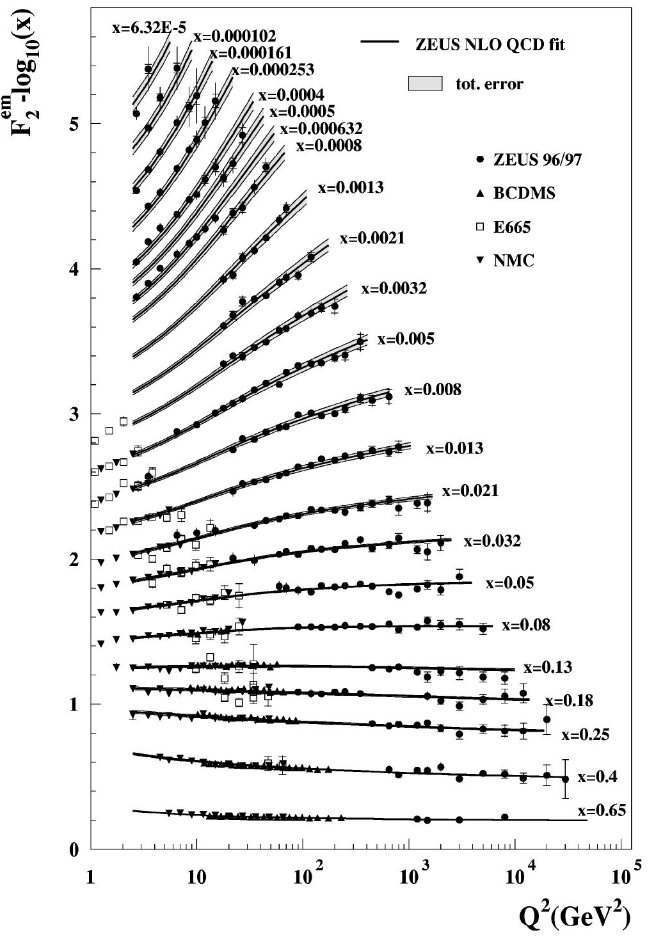
\includegraphics[width=0.5\textwidth]{Figures/WBoson/Theory/Structure_Function.png}
 \end{center}
\caption{NLO QCD fits to the to the ZEUS $F_{2}$ structure function data from 1996, 1997 and proton fixed-target at HERA. The error bands of the fit represent the total experimental uncertainty from both correlated and uncorrelated sources. Figure taken from Ref.~\cite{HERAStrucFunc}}
 \label{fig:HERAStrucFunc}
\end{figure}

The DIS process consists in the inelastic scattering of electrons off protons as presented in \fig{dia:DIS}. In the DIS process, the momentum transferred from the electron to the proton is defined as $Q^{2} = -q^{2} = -\left(k - k'\right)^{2}$ and the corresponding Bjorken x fraction is $x = {Q^{2}}\big/{2\left(p^{h}_{in}.q\right)}$. Even though DIS experiments were not able to probe the gluons directly, the DIS data showed that valence quarks did only carry half of the proton momentum been the rest carried by the gluons.

\begin{figure}[htbp]
  \vspace{10mm}
  \begin{center}
  \begin{fmffile}{DIS}
    \begin{fmfgraph*}(160,100)
      \fmfleft{ip,il}
      \fmfright{x1,x2,x3,o1,o2,o3,o4,ol}
      \fmfset{arrow_len}{10}
      % lepton
      \fmflabel{$\text{e}^-$}{il}
      \fmflabel{$\text{e}^-$}{ol}
      \fmf{fermion,label=$k$, label.side=left}{il,vl}
      \fmf{fermion,label=$k'$,label.side=left}{vl,ol}
      \fmf{phantom,tension=0.6}{vl,vp}
      % proton
      \fmfv{l=$\text{p}^+$,l.a=-160}{ip} % l.a = label.angle
      \fmf{phantom,tension=1}{ip,vp,x1}
      \fmffreeze
      \fmfi{fermion}{vpath (__ip,__vp) scaled 1.01}
      \fmfi{fermion,label=$p$,label.side=left}
                    {vpath (__ip,__vp) scaled 1.01 shifted (-1.4, 6)}
      \fmfi{fermion}{vpath (__ip,__vp) scaled 1.01 shifted ( 1.4,-6)}
      \fmfblob{25}{vp}
      % X
      \fmfv{l=\mybrace{40} $X$,l.a=10}{x2}
      \fmf{fermion}{vp,x1}
      \fmf{phantom}{vp,x2} % to help \fmfi
      \fmfi{fermion}{vpath (__vp,__x2) scaled 0.98 shifted (0,2.2)}
      \fmffreeze
      % photon
      \fmf{photon,label=\vspace{-4pt}\hspace{5pt}{$q$},label.side=left}{vl,v}
      % parton
      \fmf{fermion,label=$xp$,label.side=left}{vp,v}
      \fmf{fermion}{v,o2}
    \end{fmfgraph*}
  \end{fmffile}
  \end{center}
  \caption{Feynman diagram of deep inelastic scattering of electrons against protons}
  \label{dia:DIS}
\end{figure}

Another important process that takes place in hadron colliders is the Drell-Yan (DY) production.  In the DY process a quark from one hadron and an antiquark from another hadron annihilate into a virtual photon ($\gamma^{*}$) or {\PZ} boson which then decays to a pair of leptons as shown in \fig{dia:DY}. Drell-Yan production is used to constrain the quark PDFs in a wide range of momentum fraction x depending on the invariant mass of the dilepton pair. In addition, the Drell-Yan process also contributes to the background of the {\PW} boson production when one the DY final state leptons is generated outside of the detector acceptance.

\begin{figure}[htbp]
  \vspace{10mm}
  \begin{center}
\begin{fmffile}{DY}
  \begin{fmfgraph*}(160,160)
    \fmfleft{i1,iq,i2,ip,i3}
    \fmfright{y1,y2,y3,o1,f1,o2,o3,o4,f2,o5,x3,x2,x1}
    \fmfset{arrow_len}{10}
    % skeleton
    \fmf{phantom,tension=0.48}{vq,vp}
    \fmf{phantom}{ip,vp,x1}
    \fmf{phantom}{iq,vq,y1}
    \fmffreeze
    % parton
    \fmfv{l=$x_1p_1$,l.a=-90,l.d=22}{vp} % cheat: actually a line label
    \fmfv{l=$x_2p_2$,l.a=90,l.d=22}{vq} % cheat: actually a line label
    \fmf{fermion,tension=1.6}{vp,v}
    \fmf{fermion,tension=1.6}{v,vq}
    % hard process
    \fmfshift{20 right}{f1,f2}
    \fmfv{l=$\bar{f}$}{f1}
    \fmfv{l=$f$}{f2}
    \fmf{boson,tension=2,label=$\text{Z}^0/\gamma^*$,label.side=left}{v,vf}
    \fmf{fermion,tension=2}{f1,vf,f2}
    % proton 1
    \fmfv{l=${h}_{A}$,l.a=180,l.d=10}{ip}
    \fmf{phantom}{ip,vp}
    \fmfi{fermion,l=$p_1$,l.s=left,l.d=8}
                  {vpath (__ip,__vp) scaled 1.01 shifted (-2.4, 6)}
    \fmfi{fermion}{vpath (__ip,__vp) scaled 1.01 shifted (-2.4, 0)}
    \fmfi{fermion}{vpath (__ip,__vp) scaled 1.01 shifted (-2.4,-6)}
    % proton 2
    \fmfv{l=${h}_{B}$,l.a=180,l.d=10}{iq}
    \fmf{phantom}{iq,vq}
    \fmfi{fermion}{vpath (__iq,__vq) scaled 1.01 shifted (-2.4, 6)}
    \fmfi{fermion}{vpath (__iq,__vq) scaled 1.01 shifted (-2.4, 0)}
    \fmfi{fermion,l=$p_2$,l.s=right,l.d=8}
                  {vpath (__iq,__vq) scaled 1.01 shifted (-2.4,-6)}
    % X 2
    \fmfshift{25 left}{x1}
    \fmfshift{20 left}{x2,x3}
    \fmf{phantom}{vp,x1} % to help \fmfi
    \fmf{phantom}{vp,x2} % to help \fmfi
    \fmf{phantom}{vp,x3} % to help \fmfi
    \fmfi{fermion}{vpath (__vp,__x1) scaled 1.0 shifted ( 0.0, 2.0)}
    \fmfi{fermion}{vpath (__vp,__x2) scaled 1.0 shifted ( 0.0, 0.0)}
    \fmfi{fermion}{vpath (__vp,__x3) scaled 1.0 shifted ( 0.0,-2.0)}
    \fmfblob{25}{vp}
    % X 2
    \fmfshift{25 left}{y1}
    \fmfshift{20 left}{y2,y3}
    \fmf{phantom}{vq,y1} % to help \fmfi
    \fmf{phantom}{vq,y2} % to help \fmfi
    \fmf{phantom}{vq,y3} % to help \fmfi
    \fmfi{fermion}{vpath (__vq,__y1) scaled 1.0 shifted ( 0.0,-2.0)}
    \fmfi{fermion}{vpath (__vq,__y2) scaled 1.0 shifted ( 0.0, 0.0)}
    \fmfi{fermion}{vpath (__vq,__y3) scaled 1.0 shifted ( 0.0, 2.0)}
    \fmfblob{25}{vq}
  \end{fmfgraph*}
\end{fmffile}
  \end{center}
  \caption{Feynman diagram of neutral charged Drell-Yan process}
  \label{dia:DY}
\end{figure}


We have considered until now only the structure of protons, but the nuclear enviroment of ions can also impact the production of particles. Pb ions are composed of 82 protons and 126 neutrons. The neutron PDF can be derived from the proton PDF using isospin symmetry (i.e. by exchanging the up and down quark PDFs), while assuming the same gluon PDF as in the proton. If no nuclear modifications are expected, protons and neutrons should then behave as free particles inside the nucleus, and one could simply sum the PDFs of the protons and neutrons scaled accordingly. In this case, the ratio of the PDF of protons bounded in the nucleus (nuclear PDF) over the free-proton PDF should be one.

To determine the nuclear modifications, the heavy ion measurements were first compared to results using deuterium. The European Muon Collaboration (EMC) measured the structure function of DIS in iron and deuterium targets between 1977 and 1988, and observed a depletion of the iron PDFs relative to the deuterium PDFs at $x>0.2$ (EMC region)~\cite{EMCStrucFunc_1} and at $x<0.01$ (shadowing region)~\cite{EMCStrucFunc_2}. Subsequent results found an enhancement at the intermediate region $0.01 < x < 0.2$ (antishadowing region)~\cite{NMCStrucFunc}. Since current heavy ion data is more limited than data from proton collisions, the global fits of the nuclear PDFs are less accurate than the proton PDFs.

\subsection{PDF global fits}

The parton distribution functions can not be currently determined from first principles due to the nonperturbative behaviour of the strong interactions. Nevertheless, their depencence on x can be derived by fitting observables (e.g. structure functions or asymmetries) to experimental data from different processes since PDFs do not depend on the initial hard scattering. The $Q^{2}$ dependence of the PDFs is determined using the DGLAP evolution equations. The most common processes used to constrain the PDFs correspond to Drell-Yan, DIS, vector boson and jet production, which have been measured by various experiments including data from HERA, SLAC and LHC.

There are several proton PDFs currently available. One of the most commonly used proton PDF in high energy physics nowadays is the one provided by the Collaboration of Theorists and Experimentalist (CTEQ). The most recent CTEQ PDF corresponds to CT14 published in 2016~\cite{CT14}. The global fits of CT14 PDFs include data of vector bosons and jets from LHC pp collisions at 7~\TeV and 8~\TeV, charm quark DIS production from HERA, and electron charge asymmetry from Tevatron. The x-dependence of the CT14 PDF is parameterized at low $Q^{2}$ scale by~\cite{CT14}:

\begin{equation}
xf_{a}\left(x, Q^{2}\right) = x^{c_{1}}\left(1-x\right)^{c_{2}}{P_{a}\left(x\right)}
\end{equation}

where $P_{a}$ is a polynominal with different parameters for each parton. In the case of the up and down valence quarks, $P_{a}$ is expressed as a Bernstein polynomial of fourth-order in $\sqrt{x}$. The $P_{a}$ distribution of gluon and the light sea quark PDFs is given instead by a Bernstein polynomial in $y=\left(2\sqrt{x}-x\right)$ of second-order and fourth-order, respectively. There is not enough data to constrain the strange quark and antiquark PDFs so they are assumed to be equal. In total, the CT14 PDFs are described by 26 fitting parameters including: 8 parameters for the valence quarks, 5 parameters for the gluon and 13 parameters for the sea quarks~\cite{CT14}.

The first global fit to describe leading-order nuclear effects was the EKS98 nPDF~\cite{EKS98}. The pion data collected by RHIC was later included in EPS08~\cite{EPS08}, EPS09~\cite{EPS09}, DSSZ~\cite{DSSZ} and nCTEQ15~\cite{nCTEQ15} nPDFs which provided constrains to the gluon nPDF. We will focus on the latest nuclear PDF calculations which are the EPPS16~\cite{EPPS16} and the nCTEQ15~\cite{nCTEQ15} NLO nPDFs.

The EPPS16 nPDFs~\cite{EPPS16} are derived from a global analysis of nuclear data sets published in 2017 by the group of Eskola, Paakkinen, Paukkunen and Salgado (EPPS). The EPPS16 nPDF calculations updates their previous EPS09~\cite{EPS09} global fits. EPPS16 includes five additional parameters compared to EPS09 to account for possible flavour dependence of the quark nuclear modifications. The EPPS16 global fits includes the same data sets as EPS09 (charged-lepton-nucleus DIS data from SLAC, DY dilepton production from EMC proton-nucleus collisions and inclusive pion production from RHIC deuteron-nucleus collisions), as well as the CHORUS neutrino-nucleus DIS data, low-mass DY production from RHIC pion-nucleus collisions, and the results using dijet and electroweak boson production in LHC \pPb collisions at $\sqrtsnn=5.02$~\TeV. The addition of the new LHC, RHIC and CHORUS data into the global fit is not in tension with the previous EPS09 data sets, reassuring the validity of the universality of the nPDFs. Moreover, the inclusion of the CMS measurements of dijet production in \pPb collisions at $\sqrtsnn=5.02$~\TeV highly constrained the gluon nPDF. On the other hand, the LHC measurements of the electroweak boson production in \pPb data was not able to further constrain the quark nPDF due to the limited statistical precision. The nuclear PDFs are parameterized in EPPS16 as:

\begin{equation}
  f_{i}^{p/A}\left(x,Q^{2}\right) = R_{i}^{A}\left(x,Q^{2}\right)f_{i}^{p}\left(x,Q^{2}\right)
\end{equation}

where $f_{i}^{p/A}$ represents the PDF of a proton bounded in a nucleus A, $f_{i}^{p}$ is the free proton PDF and $R_{i}^{A}$ is the corresponding nuclear modification. The EPPS16 nuclear modifications are derived using the NLO CT14 PDF as the free proton baseline. %
%The EPPS16 function used to fit the $R_{i}^{A}\left(x,Q^{2}\right)$ is shown in \fig{fig:EPPS15_RiA}. %
The parameters of $R_{i}^{A}$ are determined in three regions: the shadowing region $x\rightarrow0$, the antishadowing maximum point $x_{a}$ and the EMC minimum point $x_{e}$. The dependence on the atomic mass A is parameterized along the three x regions in the following way:

\begin{equation}
  R^{A}_{i}\left(x,Q^{2}_{0}\right) = R^{A_{\mathrm{ref}}}_{i}\left(x,Q^{2}_{0}\right)\left(\frac{A}{A_{\mathrm{ref}}}\right)^{\gamma_{i}\left[R_{i}^{A_{\mathrm{ref}}}\left(x,Q^{2}_{0}\right) - 1\right]}
\end{equation}

where $Q_{0}$ is the parameterization scale fixed at the charm pole mass (1.3~\GeV), $\gamma_{i}$ is a positive parameter and $A_{\mathrm{ref}}=12$. The $Q^{2}$ dependence above $Q^{2}_{0}$ is determined by solving the DGLAP parton evolution equations. The strong coupling constant evaluated at the {\PZ} boson mass is set to $\alpha_{s}\left(M_{Z}\right)=0.118$. The EPPS16 nuclear modifications are paremeterized in total by 20 parameters.

The nCTEQ15 nuclear PDF published by Kovarik et al. in 2016 was derived using the CTEQ framework at next-to-leading order. The nCTEQ15 nPDF global fits make use of charged-lepton DIS data, DY dilepton production and RHIC inclusive pion production. In contrast with EPPS16 where the nuclear modification factor $R_{i}^{p/A}$ is fitted, the nCTEQ15 global analysis parametrizes  the nuclear PDF $f_{i}^{p/A}$ directly (i.e. no free proton PDF is used as baseline). The nCTEQ nPDFs are parameterized as:

\begin{equation}
  \begin{alignedat}{1}
    xf_{i}^{p/A}\left(x,Q_{0}\right) &= c_{0}x^{c_{1}}\left(1-x\right)^{c_{2}}e^{c_{3}x}\left(1+e^{x_{4}}x\right)^{c_{5}} \\
    \frac{\bar{d}\left(x,Q_{0}\right)}{\bar{u}\left(x,Q_{0}\right)} &= c_{0}x^{c_{1}}\left(1-x\right)^{c_{2}} + \left(1+c_{3}x\right)\left(1-x\right)^{c_{4}} \\
    s^{p/A}\left(x,Q_{0}\right) &= \bar{s}^{p/A}\left(x,Q_{0}\right) = \frac{\kappa\left(A\right)}{2}\left(\bar{u}^{p/A}\left(x,Q_{0}\right) + \bar{d}^{p/A}\left(x,Q_{0}\right)\right)
  \end{alignedat}
\end{equation}

where $f_{i}^{p/A}$ is defined for $i = \left(u_{v} , d_{v} , g , \bar{u}+\bar{d} , s+\bar{s} , s-\bar{s}\right)$, $\kappa\left(A\right)=\left(c^{s+\bar{s}}_{0,0} + c^{s+\bar{s}}_{0,1}\left(1-A^{-c^{s+\bar{s}}_{0,2}}\right)\right)$ and the parameterization scale $Q_{0}=1.3$~\GeV. The A-dependence of the nCTEQ15 nPDF is parameterized directly in the coeficients using $c_{k}\left(A\right) = c_{k,0} + c_{k,1}\left(1-A^{-c_{k,2}}\right)$, where $k=1,...,5$.

The nCTEQ15 global fits to the data sets are performed by minimazing the $\chi^{2}$. The nCTEQ15 fits are performed using 16 free parameters separated in: 7 gluon, 4 up valence quark, 3 down valence quark and 2 $\left(d+u\right)$ antiquark parameters. Also, nCTEQ15 treat the light valence quark densities independently but it assume no flavour dependence of the light antiquark nuclear modifications. The nCTEQ15 calculations avoid fitting the low $Q^{2}$ and high x region $x>0.7$ since this region is very difficult to model theoretically due to the presence of target mass corrections, large x resummation, nuclear off-shell effects and Fermi motion effects which steeply rise the parton densities when approaching $x=1$.

The PDF uncertainties are determined using the Hessian matrix approach. The main idea of the Hessian method is that the distribution of the $\chi^{2}\left(\{a_{i}\}\right)$ around its minimum $\chi^{2}\left(\{a^{0}_{i}\}\right)$ can be approximately parameterized by a quadratic function of the $n$ fitting parameters $\{a_{i}\}$ as $\chi^{2}\left(\{a_{i}\}\right)\approx{\chi^{2}\left(\{a^{0}_{i}\}\right)}\sum_{i,j}y_{i}H_{i,j}y_{j}$ where $y_{i}=a_{i}-a_{i}^{0}$ and $H_{i,j}=\left(1/2\right)\left(d^{2}\chi^{2}/dy_{i}dy_{j}\right)_{a_{i}=a_{i}^{0}}$ is the Hessian matrix that encodes the impact of variations around each parameter. Since $H_{i,j}$ is a symmetric matrix, it has n orthogonal eigenvectors. The eigenvectors of $H_{i,j}$ are used to define a new basis $\{z_{k}\}$ which  transform $H$ into a diagonal matrix. In order to compute the PDF uncertainties, the EPPS16 and nCTEQ15 calculations provide the PDF central set $S_{0}$ and the PDF error sets $S^{\pm}_{k}$ defined in the $\{z_{k}\}$ coordinates. Each $S^{\pm}_{k}$ is determined by evaluating the PDF on $\{z^{\pm}_{k}\}$ defined by varying upward/downward the parameter $\{z_{k}\}$ along the k-th eigenvector direction as:

\begin{equation}
  S^{\pm}_{k} = f\left(z^{0}_{k} \pm \sqrt{\frac{\Delta{\chi^{2}}}{\lambda_{k}}}\right)
\end{equation}

where $\lambda_{k}$ is the k-th eigenvalue of $H$ and $\Delta{\chi^{2}}$ is the tolerance criterion defined at $90\%$ confidence limit. In nCTEQ15 the tolerance is set to $\Delta{\chi^{2}}=35$ while in EPPS16 it is set to $\Delta{\chi^{2}}=??$. Using the PDF error sets, the PDF uncertainties can then be definied as:

\begin{equation}
  \Delta{O} = \sqrt{\sum_{i}\left[{\vphantom{P}^{\mathrm{max}}_{\mathrm{min}}}\left\{O\left(S_{i}^{+}\right) - O\left(S_{i}^{0}\right), O\left(S_{i}^{-}\right) - O\left(S_{i}^{0}\right), 0\right\}\right]^{2}}
\end{equation}

To derive the correlation between two observables $X$ and $Y$, one can use the cosine of the correlation angle define as:

\begin{equation}
  \mathrm{cos}{\phi\left[X,Y\right]} = \frac{\sum_{i_{\mathrm{PDF}}}\left(X^{+}_{i_{\mathrm{PDF}}} - X^{-}_{i_{\mathrm{PDF}}}\right)}{\left(Y^{+}_{i_{\mathrm{PDF}}} - Y^{-}_{i_{\mathrm{PDF}}}\right)}{\sqrt{\sum_{j_{\mathrm{PDF}}}\left(X^{+}_{j_{\mathrm{PDF}}} - X^{-}_{j_{\mathrm{PDF}}}\right)^{2}}\sqrt{\sum_{k_{\mathrm{PDF}}}\left(Y^{+}_{k_{\mathrm{PDF}}} - Y^{-}_{k_{\mathrm{PDF}}}\right)^{2}}}
\end{equation}

where the observables are calculated over the upward/downward PDF error sets in each eigenvector direction (16 for nCTEQ15 and 20 for EPPS16). The main differences between the EPS09, EPPS16 and nCTEQ15 nuclear PDFs are summarized in \tab{tab:nPDFInfo}.

\begin{table}[htbp]
  \begin{center}
    \begin{tabular}{ c | c c c }
    nPDF & EPS09 & EPPS16 & nCTEQ15 \\ \hline
    Order & NLO & NLO & NLO \\
    Fit & nucler modification & nuclear modification & nuclear PDF \\
    Baseline PDF & CT14 & CTEQ6 & \\
    Free parameters & 15 & 20 & 17 \\
    Data points & 929 & 1811 & 708 \\
    EMC DY dileptons in p-A & Yes & Yes & Yes \\
    RHIC pions in d-A & Yes & Yes & Yes \\
    SLAC $l^{\pm}$-A DIS & Yes & Yes & Yes \\
    CHORUS $\nu$-A DIS & No & Yes & No \\
    RHIC DY in $\pi$-A & No & Yes & No \\
    LHC dijets in \pPb & No & Yes & No \\
    LHC weak bosons in \pPb & No & Yes & No
    \end{tabular}
  \end{center}
  \label{tab:nPDFInfo}
  \caption{Summary of the information of EPS09, EPPS16 and nCTEQ15 nuclear PDFs.}
\end{table}

%The current nPDF calculations that are less constrained include the flavour dependence of valence quark nuclear modifications, sea quark PDFs at $x<10^{-2}$ and the strange quark nuclear PDFs. Therefore,  using the recent LHC \pPb data at 8.16~\TeV, one could further constrain the valence and sea quark nuclear PDFs by measuring the low-mass DY dilepton production and the {\PW} boson production. The strange quark nuclear PDF can be constrained from the measurement of the production of {\PW} bosons in association with charm quarks in \pPb collisions. In this thesis we present the measurements of the inclusive {\PW} boson production in \pPb collisions at 8.16~\TeV.



\subsection{Production of W bosons at LHC}

The production of {\PW} bosons in hadronic collisions is accomplished through the process of quark-antiquark annihilation. The measurement of {\PW} boson production in \pPb collisions at $\sqrtsnn=8.16$~\TeV is performed in the semimuonic decay channel. At leading order (LO), the {\PW} boson hadroproduction to final state leptons is described by the Feynman diagram shown in \fig{dia:WProd}.

\begin{figure}[htbp]
  \vspace{10mm}
  \begin{center}
  \begin{fmffile}{WProd}
  \begin{fmfgraph*}(160,160)
    \fmfleft{i1,iq,i2,ip,i3}
    \fmfright{y1,y2,y3,o1,f1,o2,o3,o4,f2,o5,x3,x2,x1}
    \fmfset{arrow_len}{10}
    % skeleton
    \fmf{phantom,tension=0.48}{vq,vp}
    \fmf{phantom}{ip,vp,x1}
    \fmf{phantom}{iq,vq,y1}
    \fmffreeze
    % parton
    \fmfv{l=$x_1p_1$,l.a=-90,l.d=22}{vp} % cheat: actually a line label
    \fmfv{l=$x_2p_2$,l.a=90,l.d=22}{vq} % cheat: actually a line label
    \fmf{fermion,tension=1.6}{vp,v}
    \fmf{fermion,tension=1.6}{v,vq}
    % hard process
    \fmfshift{20 right}{f1,f2}
    \fmfv{l=$\bar{\nu}_{\ell}$}{f1}
    \fmfv{l=$\ell^{\pm}$}{f2}
    \fmf{boson,tension=2,label=$\text{W}^{\pm}$,label.side=left}{v,vf}
    \fmf{fermion,tension=2}{f1,vf,f2}
    % proton 1
    \fmfv{l=p,l.a=180,l.d=10}{ip}
    \fmf{phantom}{ip,vp}
    \fmfi{fermion,l=$p_1$,l.s=left,l.d=8}
                  {vpath (__ip,__vp) scaled 1.01 shifted (-2.4, 6)}
    \fmfi{fermion}{vpath (__ip,__vp) scaled 1.01 shifted (-2.4, 0)}
    \fmfi{fermion}{vpath (__ip,__vp) scaled 1.01 shifted (-2.4,-6)}
    % proton 2
    \fmfv{l=Pb,l.a=180,l.d=10}{iq}
    \fmf{phantom}{iq,vq}
    \fmfi{fermion}{vpath (__iq,__vq) scaled 1.01 shifted (-2.4, 6)}
    \fmfi{fermion}{vpath (__iq,__vq) scaled 1.01 shifted (-2.4, 0)}
    \fmfi{fermion,l=$p_2$,l.s=right,l.d=8}
                  {vpath (__iq,__vq) scaled 1.01 shifted (-2.4,-6)}
    % X 2
    \fmfshift{25 left}{x1}
    \fmfshift{20 left}{x2,x3}
    \fmf{phantom}{vp,x1} % to help \fmfi
    \fmf{phantom}{vp,x2} % to help \fmfi
    \fmf{phantom}{vp,x3} % to help \fmfi
    \fmfi{fermion}{vpath (__vp,__x1) scaled 1.0 shifted ( 0.0, 2.0)}
    \fmfi{fermion}{vpath (__vp,__x2) scaled 1.0 shifted ( 0.0, 0.0)}
    \fmfi{fermion}{vpath (__vp,__x3) scaled 1.0 shifted ( 0.0,-2.0)}
    \fmfblob{25}{vp}
    % X 2
    \fmfshift{25 left}{y1}
    \fmfshift{20 left}{y2,y3}
    \fmf{phantom}{vq,y1} % to help \fmfi
    \fmf{phantom}{vq,y2} % to help \fmfi
    \fmf{phantom}{vq,y3} % to help \fmfi
    \fmfi{fermion}{vpath (__vq,__y1) scaled 1.0 shifted ( 0.0,-2.0)}
    \fmfi{fermion}{vpath (__vq,__y2) scaled 1.0 shifted ( 0.0, 0.0)}
    \fmfi{fermion}{vpath (__vq,__y3) scaled 1.0 shifted ( 0.0, 2.0)}
    \fmfblob{25}{vq}
  \end{fmfgraph*}
  \end{fmffile}
  \end{center}
  \caption{Feynman diagram of LO {\PW} boson production to final state leptons in \pPb collisions}
  \label{dia:WProd}
\end{figure}


In this thesis, the cross section of the {\PW} boson production is measured in \pPb collisions as a function of muon pseudorapidity ($\eta$) considering muons with \pt larger than 25~\GeVc. The  theoretical cross section can be derived using electroweak theory and the factorization theorem shown in \eq{eq:FactTheorem}. The {\PW} boson hadroproduction cross section has been calculated in Ref.~\cite{WProdScaling}, and the corresponding \pPb LO differential cross section as a function of muon $\eta$, considering $\Gamma_{\PW}<<M_{\PW}$, is:

\begin{equation}
  \begin{split}
    \frac{d\sigma^{\PW^{\pm}}}{d\eta}\left(\snn\right) &\approx
    \frac{\pi^{2}}{6{M^{5}_{\PW}}{\Gamma_{W}}}
    \left(\frac{\alpha_{em}}{\mathrm{sin}^{2}\left(\theta_{\PW}\right)}\right)^{2}
    \int_{25}^{\inf}d\pt
    \frac{\pt^{3}}{\sqrt{1-4\pt^{2}/M_{\PW}^{2}}}
    \sum_{i,j}
    \delta\left(e_{q_{i}}+e_{\bar{q}_{j}}, \pm{1}\right)
    {\left|V^{\mathrm{CKM}}_{ij}\right|^{2}} \\
    \left\{ \vphantom{x_{2}^{\pm}q_{j}^{\mathrm{Pb}}} \right. &\left.
    x_{\mathrm{p}}^{\pm}q_{i}^{\mathrm{p}}\left(x_{\mathrm{p}}^{+},Q^{2}\right) \cdot x_{\mathrm{Pb}}^{\mp}\bar{q}_{j}^{\mathrm{Pb}}\left(x_{\mathrm{Pb}}^{+},Q^{2}\right) + 
    x_{\mathrm{p}}^{\pm}\bar{q}_{i}^{\mathrm{p}}\left(x_{\mathrm{p}}^{-},Q^{2}\right) \cdot x_{\mathrm{Pb}}^{\mp}q_{j}^{\mathrm{Pb}}\left(x_{\mathrm{Pb}}^{-},Q^{2}\right) + {} \right. \\ &\left.
    x_{\mathrm{p}}^{\mp}q_{i}^{\mathrm{p}}\left(x_{\mathrm{p}}^{-},Q^{2}\right) \cdot x_{\mathrm{Pb}}^{\pm}\bar{q}_{j}^{\mathrm{Pb}}\left(x_{\mathrm{Pb}}^{-},Q^{2}\right) + 
    x_{\mathrm{p}}^{\mp}\bar{q}_{i}^{\mathrm{p}}\left(x_{\mathrm{p}}^{+},Q^{2}\right) \cdot x_{\mathrm{Pb}}^{\pm}q_{j}^{\mathrm{Pb}}\left(x_{\mathrm{Pb}}^{+},Q^{2}\right)
    \right\}
  \end{split}
  \label{eq:WProd}
\end{equation}

where $\alpha_{em}$ is the fine-structure constant, $q^{\mathrm{p}}$ is the free-proton quark PDF, $q_{i}^{\mathrm{Pb}}$ is the Pb nuclear quark PDF, and $Q\approx{M_{\PW}}$ is the momentum scale. The sum in \eq{eq:WProd} is performed over all quark flavours and the parton momemtum fraction variables $x_{\mathrm{p}}$ and $x_{\mathrm{Pb}}$ are defined as~\cite{WProdScaling}:

\begin{equation}
  \begin{alignedat}{2}
    x_{\mathrm{p}}^{\pm} &= \frac{M_{\PW}}{\sqrtsnn} e^{\eta} &&\left[\frac{1 \mp \sqrt{1 - 4\pt^{2}/M_{\PW}^{2}}}{2\pt/M_{\PW}}\right] \\
    x_{\mathrm{Pb}}^{\pm} &= \frac{M_{\PW}}{\sqrtsnn} e^{-\eta} &&\left[\frac{1 \pm \sqrt{1 - 4\pt^{2}/M_{\PW}^{2}}}{2\pt/M_{\PW}}\right]
  \end{alignedat}
  \label{eq:WProdBjorkenX}
\end{equation}

The cross sections of negative and positive charged leptons, shown in \eq{eq:WProd}, are different due to parity violation and helicity conservation of weak decays. Since $\PW^{+}$ bosons couple to right-handed leptons while $\PW^{-}$ couples to left-handed leptons, leptons are produced in the same direction as the {\PW} boson while antileptons are generated in the opposite direction. This is reflected in \eq{eq:WProdBjorkenX} where $\mu^{-}$ production is sensitive to slightly higher x than $\mu^{+}$ production.

Multiple proton-proton and proton-neutron hard scatterings takes place during \pPb collisions. In this case, the {\PW} bosons are mainly produced from interactions between the valence quarks and sea antiquarks of the nucleons. The dominant production modes of $\PW^{+}$ bosons correspond to up quark and down antiquark annihilation while for $\PW^{-}$ bosons correspond to down quark and up antiquark annihilation. The annihilation between light quarks and heavier antiquarks is also possible but highly suppressed according to the CKM matrix elements. Therefore, the inclusive {\PW} boson cross section measured in \pPb data is mostly sensitive to the proton and Pb-nucleus PDFs of light quarks and antiquarks.

In addition, the {\PW} boson cross sections can be compared between different beam energies. According to Arleo and Chapon~\cite{WProdScaling}, at small enough x values, the {\PW} boson cross section follows a power-like scaling as a function of $\snn$, where \eq{eq:WProd} can be approximately reduced to:

\begin{equation}
  \begin{alignedat}{2}
    \frac{d\sigma^{\PW^{\pm}}}{d\eta}\left(\snn, \xi_{\mathrm{p }}\right) &\approx \left({\snn}\right)^{\alpha} \times F^{\pm}_{\mathrm{p,Pb}}\left(\xi_{\mathrm{p}} , \pt\right), &&\ \ \ \eta>>0, \\
    \frac{d\sigma^{\PW^{\pm}}}{d\eta}\left(\snn, \xi_{\mathrm{Pb}}\right) &\approx \left({\snn}\right)^{\alpha} \times G^{\pm}_{\mathrm{p,Pb}}\left(\xi_{\mathrm{Pb}}, \pt\right), &&\ \ \ \eta<<0
  \end{alignedat}
  \label{eq:WProdScaling}
\end{equation}

where $\alpha$ is the scaling parameter, and $\xi_{p} = \left(M_{\PW}\big/\sqrtsnn\right)e^{-\eta}$ and $\xi_{Pb} = \left(M_{\PW}\big/\sqrtsnn\right)e^{\eta}$ are the x values at $\pt=M_{\PW}/2$ in the proton and Pb ion, respectively. Moreover, the functions $F^{\pm}_{\pPb}$ and $G^{\pm}_{\pPb}$ do not depend explicitely on $s$ or $\eta$.

Furthermore, since the scaling parameter does not depend on the lepton pseudorapidity or the charge of the {\PW} boson, the dependence on $\snn$ cancels in ratios of {\PW} boson cross sections. We can then measure assymmetries to improve the sensitivity to different aspects of the {\PW} boson production. Two of the most commonly used are the lepton charge asymmetry defined in \eq{eq:MuonChargeAsymmetry} and the forward-backward ratio presented in \eq{eq:MuonForwardBackwardAsymmetry}. Thus, according to \eq{eq:WProdScaling}, the {\PW} boson asymmetries only depends on $\xi_{\mathrm{p}}$ and $\xi_{\mathrm{Pb}}$ for $|\eta|>>0$.


% END OF SECTION


\clearpage

\section{Dataset and simulated samples} \label{sec:WBoson_Samples}

\subsection{Dataset} \label{sec:WBoson_Samples_Data}

The primary dataset used for the \W analysis is PASingleMuon. The dataset contains events from \pPb collisions at 8.16~\TeV recorded by the CMS detector requiring at least one identified muon. The data were reconstructed with the CMS software version 8.0.30 and was thoroughly validated by the CMS collaboration. Only runs passing the data quality requirements were processed. The total integrated luminosity of the recorded data corresponds to 173.4~\nbinv, currently known within 5$\%$~\cite{LUMI}.

In the first part of the \pPb run (labelled as \RunPbp), the proton was heading towards negative pseudorapidity $-\eta$, according to the CMS detector convention~\cite{CMS}, with an energy of 6.5~\TeV and colliding a lead nuclei at 2.56~\TeV~\cite{LHC}. In the second part of the \pPb run (labelled as \RunpPb), the proton was going towards $+\eta$, still boosted compared to the lead nuclei. The integrated luminosity of the \RunPbp and \RunpPb runs were 62.6~\nbinv and 110.8~\nbinv, respectively.

%%------------------------------------------------------------%%
\subsection{Next-to-leading order simulations} \label{sec:WBoson_Sample_MC}

Fully reconstructed Monte Carlo (MC) simulated samples are used to describe the signal and the different sources of Electro-Weak (EWK) backgrounds. The MC samples were generated at Next-to-Leading order (NLO) using the POsitive Weight Hardest Emission Generator (\POWHEG)~\cite{POWHEG,POWHEG_2,POWHEGBOX} version 2. To account for Quantum Chromo-Dynamic (QCD) and EWK corrections, the \POWHEGBOX  packages \verb#W_ew-BMMNP#~\cite{POWHEGBOX_W_ew_BMNNP} and \verb#Z_ew-BMMNPV#~\cite{POWHEGBOX_Z_ew_BMNNP} were used to generate the $\pp\to\W\to l\PGnl$ and $\pp\to\DY\to l^{+}l^{-}$ processes, respectevely. The $\pp\to\ttbar$ was generated using the \POWHEGBOX package \verb#hvq#~\cite{POWHEGBOX_hvq}, which is a heavy flavour quark generator at NLO QCD. 

Since the data is based on \pPb collisions, the simulation of both proton-proton (\pp) and proton-neutron (\pn) collisions is crucial. In order to simulate \pPb collisions and also include nuclear modifications to the PDFs, the \POWHEG framework was modified. This was done by first generating \pp collisions using the CT14 parton distribution function~\cite{CT14}. Then each PDF was corrected by applying the EPPS16 nuclear modification factors derived for Pb ions~\cite{EPPS16}. And finally, the \cPqu-quark and \cPqd-quark PDFs were scaled considering the number of neutrons and protons in the Pb nucleus. The nuclear modification and normalization of the quark PDFs is shown in \eq{eq:PbScaling}.

\begin{equation}
\begin{aligned}
f^{\cPqu}_{Pb} &= \frac{Z}{A}\left[R^{\cPqu}_{s}f^{\cPaqu}_{\Pp} + R^{\cPqu}_{v}\left(f^{\cPqu}_{\Pp}-f^{\cPaqu}_{\Pp}\right)\right] + \frac{A-Z}{A}\left[R^{\cPqd}_{s}f^{\cPaqd}_{\Pp} + R^{\cPqd}_{v}\left(f^{\cPqd}_{\Pp}-f^{\cPaqd}_{\Pp}\right)\right] \\
f^{\cPqd}_{Pb} &= \frac{Z}{A}\left[R^{\cPqd}_{s}f^{\cPaqd}_{\Pp} + R^{\cPqd}_{v}\left(f^{\cPqd}_{\Pp}-f^{\cPaqd}_{\Pp}\right)\right] + \frac{A-Z}{A}\left[R^{\cPqu}_{s}f^{\cPaqu}_{\Pp} + R^{\cPqu}_{v}\left(f^{\cPqu}_{\Pp}-f^{\cPaqu}_{\Pp}\right)\right]
\end{aligned}
\label{eq:PbScaling}
\end{equation}

where $f$ represent the quark PDF, $R_{s}$ ($R_{v}$) is the nuclear modification factor for sea (valence) quarks, A is the Pb mass number and Z is the Pb atomic number.

The parton showering is performed by hadronizing the \POWHEG events in \PYTHIA 8.212~\cite{PYTHIA8} with the CUETP8M1 underlying event (UE) tune~\cite{PYTHIA_TUNE,UE_pp}. The decay of \PGt particles is handled in \PYTHIA using the \TAUOLA C++ Interface 1.1.5~\cite{TAUOLA}, including final state radiative (FSR) QED corrections using~\PHOTOS 2.15 \cite{PHOTOS}. The full CMS detector response is simulated in all MC samples, based on \GEANTfour~\cite{GEANT4}, considering a realistic aligment and calibration of the beam spot and the different sub-detectors of CMS, tuned on data. The MC events are reconstructed with the standard CMS \pp reconstruction software used during 2016 data taking.

To consider a more realistic distribution of the underlying environment present in the \pPb collisions, the MC signal events were embedded in a minimum bias sample generated with \EPOS~\cite{EPOS}, taking into account the \pPb boost direction. The EPOS MC samples were tuned to reproduce the global event properties of the \pPb data such as the charged-hadron transverse momentum spectrum and the particle multiplicity \cite{dNdEta_pPb}. The list of simulated samples and the corresponding cross sections used are summarized in \tab{tab:MCSamples}.

\begin{table} [h!]
  \centering
  \resizebox{\textwidth}{!}{
    \renewcommand{\arraystretch}{1.5}
    \begin{tabular}{c c c c c c}
      \hline
      Process & Criteria & Generator & PDF & Cross section (nb) & Events \\
      \hline
      $\pPb \to \WToMuNuPl$ & & \POWHEG+\PYTHIA & CT14+EPPS16 & 1213.4 (NLO) & 982714  \\
      $\Pbp \to \WToMuNuPl$ & & \POWHEG+\PYTHIA & CT14+EPPS16 & 1214.1 (NLO) & 981874  \\
      $\pPb \to \WToMuNuMi$ & & \POWHEG+\PYTHIA & CT14+EPPS16 & 1082.2 (NLO) & 995726  \\
      $\Pbp \to \WToMuNuMi$ & & \POWHEG+\PYTHIA & CT14+EPPS16 & 1083.4 (NLO) & 998908  \\
      \hline
      $\pPb \to \WToTauNuPl$ & & \POWHEG+\TAUOLA & CT14+EPPS16 & 1146.3 (NLO) & 481125  \\
      $\Pbp \to \WToTauNuPl$ & & \POWHEG+\TAUOLA & CT14+EPPS16 & 1147.4 (NLO) & 500000  \\
      $\pPb \to \WToTauNuMi$ & & \POWHEG+\TAUOLA & CT14+EPPS16 & 1026.3 (NLO) & 495450  \\
      $\Pbp \to \WToTauNuMi$ & & \POWHEG+\TAUOLA & CT14+EPPS16 & 1019.4 (NLO) & 498092  \\
      \hline
      $\pPb \to \DYToMuMu$ & $10<M_{\DY}<30$ & \POWHEG+\PYTHIA & CT14+EPPS16 & 1182.2 (NLO) & 997120  \\
      $\Pbp \to \DYToMuMu$ & $10<M_{\DY}<30$ & \POWHEG+\PYTHIA & CT14+EPPS16 & 1168.0 (NLO) & 1000000 \\
      $\pPb \to \DYToMuMu$ & $30<M_{\DY}<\infty$ & \POWHEG+\PYTHIA & CT14+EPPS16 & 266.3 (NLO) & 1000000  \\
      $\Pbp \to \DYToMuMu$ & $30<M_{\DY}<\infty$ & \POWHEG+\PYTHIA & CT14+EPPS16 & 266.3 (NLO) & 1000000  \\
      \hline
      $\Pbp \to \DYToTauTau$ & $10<M_{\DY}<30$ & \POWHEG+\TAUOLA & CT14+EPPS16 & 1143.7 (NLO) & 464494  \\
      $\Pbp \to \DYToTauTau$ & $30<M_{\DY}<\infty$ & \POWHEG+\TAUOLA & CT14+EPPS16 & 259.4 (NLO) & 498444  \\
      \hline
      $\pPb \to \ttbar$ & & \POWHEG+\PYTHIA & CT14+EPPS16 & 45 (CMS) & 99578  \\
      $\Pbp \to \ttbar$ & & \POWHEG+\PYTHIA & CT14+EPPS16 & 45 (CMS) & 100000  \\
      \hline
    \end{tabular}
  }
  \caption{Simulated NLO samples used for the \W boson measurement in \pPb at 8.16~\TeV. The listed cross sections are the \POWHEG generator cross sections scaled by 208 (atomic number of Pb ion), except for \ttbar cross sections which are taken from the latest measurement in \pPb at 8.16\TeV by CMS \cite{HIN-17-002}.}
  \label{tab:MCSamples}
\end{table}
  
%%------------------------------------------------------------%%
\subsection{Center of Mass Frame} \label{sec:WBoson_Sample_CMFrame}
  
Due to the energy difference between the \pPb colliding beams, the nucleon-nucleon center-of-mass (CM) frame was not at rest with respect to the laboratory (LAB) frame. Massless particles emitted at a pseudorapidity $\eta_{CM}$ in the CM frame experienced a longitudinal boost as described in equation \ref{eq:CMShift}.

\begin{equation}
\abs{\Delta{\eta}_{CM}} = \frac{1}{2}\times\left|\ln\left(\frac{Z_{Pb}\times A_{p}}{Z_{p}\times A_{Pb}}\right)\right| = \frac{1}{2}\times\ln\left(\frac{208}{82}\right) = 0.465
\label{eq:CMShift}
\end{equation}

The shift between the CM and LAB frames depends on the orientation of the beams, and are applied in the following way:

\begin{itemize}
\item \RunPbp\ (1st run): $\eta_{LAB} = \eta_{CM} - 0.465$
\item \RunpPb\ (2nd run): $\eta_{LAB} = \eta_{CM} + 0.465$
\end{itemize}


%%------------------------------------------------------------%%
\subsection{Combining \pPb runs} \label{sec:WBoson_Sample_CombiningBeamDirection}

Since the CMS detector is symmetric with respect to the beam orientation, the \RunpPb and \RunPbp samples are merged in order to maximize the statistics of the MC simulations and the data. This is done by first flipping the sign of the pseudorapidity of particles from the \RunPbp sample measured in the laboratory frame, and then combine them with the events from the \RunpPb sample. In the case of the MC samples, the events are reweighed before merging them, so that the simulated luminosity match the integrated luminosity recorded in each proton-lead run. The combined sample is labelled as "pA" and corresponds to \pPb collisions with the proton always going toward $+\eta$.


% END OF SUBSECTION






\section{Event selection} \label{sec:WBoson_Selection}


The \W boson yields are measured in the semi-muonic decay channel. The signal events, determined by the process \WToMuNu, are characterised by a high transverse momentum (\pt) muon and the presence of missing tranverse energy (\ETslash\ ), originated from the undetected neutrino. Moreover, events with similar characteristics can also be produced by other background processes, such as multi-jet events, Drell-Yan dilepton events or EWK decays. This section explain the different selections implemented to supress the background and enhance the signal.

%%------------------------------------------------------------%%
\subsection{\pPb global filter} \label{sec:WBoson_Selection_EventFilter}

In order to ensure that the samples are not contaminated by non-collision events, such as cosmics or electronic noise, a \pPb Global Event Filter (GEF) is applied. The different selections included in the \pPb GEF are described below:

\begin{itemize}
\item Primary Vertex filter: Requires a primary vertex reconstructed from at least two tracks, within a longitudinal (transverse) distance of 25~\cm (2~\cm) of the nominal interaction point.
\item HF Coincidence filter: Requires at least one tower on each side of the interaction point in the Hadron-Forward (HF) calorimeter with an energy deposit per tower of at least 3~\GeV.
\item Beam-Scraping filter: Requires at least 25$\%$ of tracks in the event to be high quality tracks.
\end{itemize}

The impact of the GEF was checked both in data and simulation. Only 0.08$\%$ of events in data and 0.06$\%$ of events in \W boson simulation, passing all the analysis cuts summarized in \sect{sec:WBoson_Selection_WSelection}, were removed by the filter.


%%------------------------------------------------------------%%
\subsection{Missing Transverse Energy} \label{sec:WBoson_Selection_MET}

Since neutrinos are not detected in the CMS detector, their presence is characterized by a particle momentum imbalance in the transverse plane, also called Missing Transverse Energy (MET). 

The MET is defined as the negative vectorial sum of the transverse momemtum of all reconstructed particles. Its coordinates along the the x and y axes in the CMS coordinate system~\cite{CMS}, can be computed as:

\begin{eqnarray*} 
\VETslash\ &=& -\sum_{particles}\ptvec \\
\ETslash\ &=& \left|\VETslash\ \right|
\end{eqnarray*}

The particle-flow algorithm (PF) \cite{PF_Reco} is used to identify the particles in the event and estimate the \ETslash\ . The PF algorithm is designed to reconstruct all stable particles such as electrons, muons, photons, charged hadrons and neutral hadrons, by taking into account all CMS sub-detectors. The outcome is an optimal determination of each particle's type, momentum and energy. This set of particles is then used to measure the \VETslash\ . The performance of the MET reconstruction in \pp data has been documented in \cite{MET_Reco,MET_PERF}.

Ideally, in an event where no neutrinos are produced, the \ETslash\ \ should be equal to zero. But since the momentum of particles is not measured with perfect precision, the sum of the reconstructed particles \ptvec does not cancel completely due to the resolution of the detector. In order to correct for the differences in the MET resolution between simulation and data, the resolution of the hadronic recoil component is smeared in the simulation to match the data as explained in \sect{sec:WBoson_Corrections_MET}.


%%------------------------------------------------------------%%
\subsection{Trigger} \label{sec:WBoson_Selection_Trigger}

The muon triggers are divided in two systems: the Level-1 (L1) trigger and the High Level Trigger (HLT). 

The L1 triggers are hardware-based and were updated during 2016 (LHC Run 2) using $\mu$TCA technology. The L1 muon trigger system is divided in 3 sub-systems: Endcap, Overlap and Barrel Muon Track Finders. The muon candidates found by each track finder are sent to the L1 Global Muon Trigger ($\mu$GMT), which process them and selects the best muon candidates. Afterwards, the L1 Global Trigger ($\mu$GT) takes the decision to either accept or reject the event based on the information provided by the $\mu$GMT and the calorimeters. In order to only consider real collisions, all \pPb L1 trigger algorithms were required to be in coincidence with a bunch crossing identified by the Beam Pick-up Timing for eXperiments (BPTX) detector. The technical information of the upgraded L1 muon trigger system is described in detail in \cite{L1_Muon_Stage2_Paper,L1_Muon_Stage2_Thesis}. 

The HLT are software-based and are only applied once an event is accepted by the L1 trigger system. The HLT muon triggers implemented for \pPb data are divided in 3 levels: the \verb#HLT_PAL1# trigger takes as input all events fired by the L1 muon trigger and does not apply any further cuts, the \verb#HLT_PAL2# trigger reconstructs the muon candidates found in the muon sub-detectors using a more sophisticated algorithm compared to L1, and the \verb#HLT_PAL3# trigger uses the muon tracks reconstructed by combining the inner tracker hits and muon tracks found by \verb#HLT_PAL2#. The HLT muon reconstruction algorithms were identical to the ones used during the 2016 \pp runs. A complete description of the CMS HLT trigger system can be found in \cite{CMS_Trigger}.

For the \W boson analysis, events that passed the muon trigger \verb#HLT_PAL3Mu12_v*# are used. This trigger requires a fully reconstructed online muon with $\pt > 12$~\GeVc. The HLT was seeded by the L1 trigger path \verb#L1_SingleMu7#, which pass events with at least one L1 muon with $\pt > 7$~\GeVc. The muon trigger was unprescaled both at L1 and HLT during the entire data taking period.

If in a given event, the main analysis trigger \verb#HLT_PAL3Mu12_v1# fired and a reconstructed muon is matched to the HLT L3 muon that fired the trigger, the reconstructed muon is considered trigger matched. The matching criteria between the reconstructed and the HLT muon is done by requiring a $\Delta{R}(\mu_{reco} , \mu_{HLT}) < 0.1$.


%%------------------------------------------------------------%%
\subsection{Muon selection} \label{sec:WBoson_Selection_MuonIdentification}

Muon candidates are identified using a tight selection optimised for muons with high \pt. The tight selection requires muon candidates to be reconstructed globally from hits in the muon stations and the tracker,  been identified with the Particle-Flow algorithm~\cite{PF_Reco} and pass the following criteria:

\begin{itemize}
\item The muon track fit has at least a $\chi^{2}$/NDF $< 10$, ensuring a reasonable fit quality.
\item The muon track has at least one hit in the muon detectors, making sure that the information from the tracker and the muon system is consistent.
\item The muon track segments are matched to at least two muon stations, making the selection consistent with the muon trigger logic.
\item The tranverse impact parameter (longitudinal distance) of the muon track is consistent with the primary vertex within 2~mm (5~mm), to reduce cosmic background and muons from decays in flight. 
\item The muon track has at least one hit in the pixel detector to further supress muons from decays in flight.
\item The muon track includes hits in at least six tracker layers to guarantee a good \pt measurement.
\end{itemize}

Apart from the muon tight selection, muon candidates are also required to be isolated in order to reduce the contribution from multi-jet background. Muons are considered isolated if the sum of the \pt of all PF particles (excluding the muon), within a cone of $\Delta{R}\left(\mu, PF\right) < 0.3$, is less than 15$\%$ of the muon \pt. The muon isolation variable is defined in \eq{eq:MuonIsolation}.

\begin{equation}
 \text{isolation} = \left(\sum_{\text{charged hadrons}}^{\text{DR}<0.3} \pt + \sum_{\text{neutral hadrons}}^{\text{DR}<0.3} \pt + \sum_{\text{photons}}^{\text{DR}<0.3} \pt\right) / \pt^\mu
 \label{eq:MuonIsolation}
\end{equation}

Since more than one muon candidate can be reconstructed in an event, the muon candidate with the highest \pt (i.e. the leading muon), is used. The event is only kept if the leading muon has a $\pt > 25$~\GeVc and $|\eta| < 2.4$. Any difference in the performance of the muon cuts observed between simulation and data, is corrected in simulation through the use of the Tag-And-Probe scale factors described in \sect{sec:WBoson_Efficiency_CorrectedEfficiency}.


%%------------------------------------------------------------%%
\subsection{Drell-Yan Veto} \label{sec:WBoson_Selection_DrellYanVeto}

A Drell-Yan veto is applied to suppress the contribution from \DYToMuMu background events. This veto removes events that contain at least two opposite sign muons with $\pt > 15$~\GeVc passing the tight muon identification and the relative muon isolation cut $iso < 0.15$, defined in \sect{sec:WBoson_Selection_MuonIdentification} .

The probability that Drell-Yan events survive the veto is checked using a Drell-Yan simulated sample. The denominator of the Drell-Yan Veto effiency is filled with the muons passing all the \W boson  analysis cuts (see \sect{sec:WBoson_Selection_WSelection}), while the numerator is filled with the same muons as long as the event pass the Drell-Yan veto. The MC survival probability is shown in \fig{fig:DrellYanVetoZEfficiency2D}.

\begin{figure}[htb]
 \begin{center}
   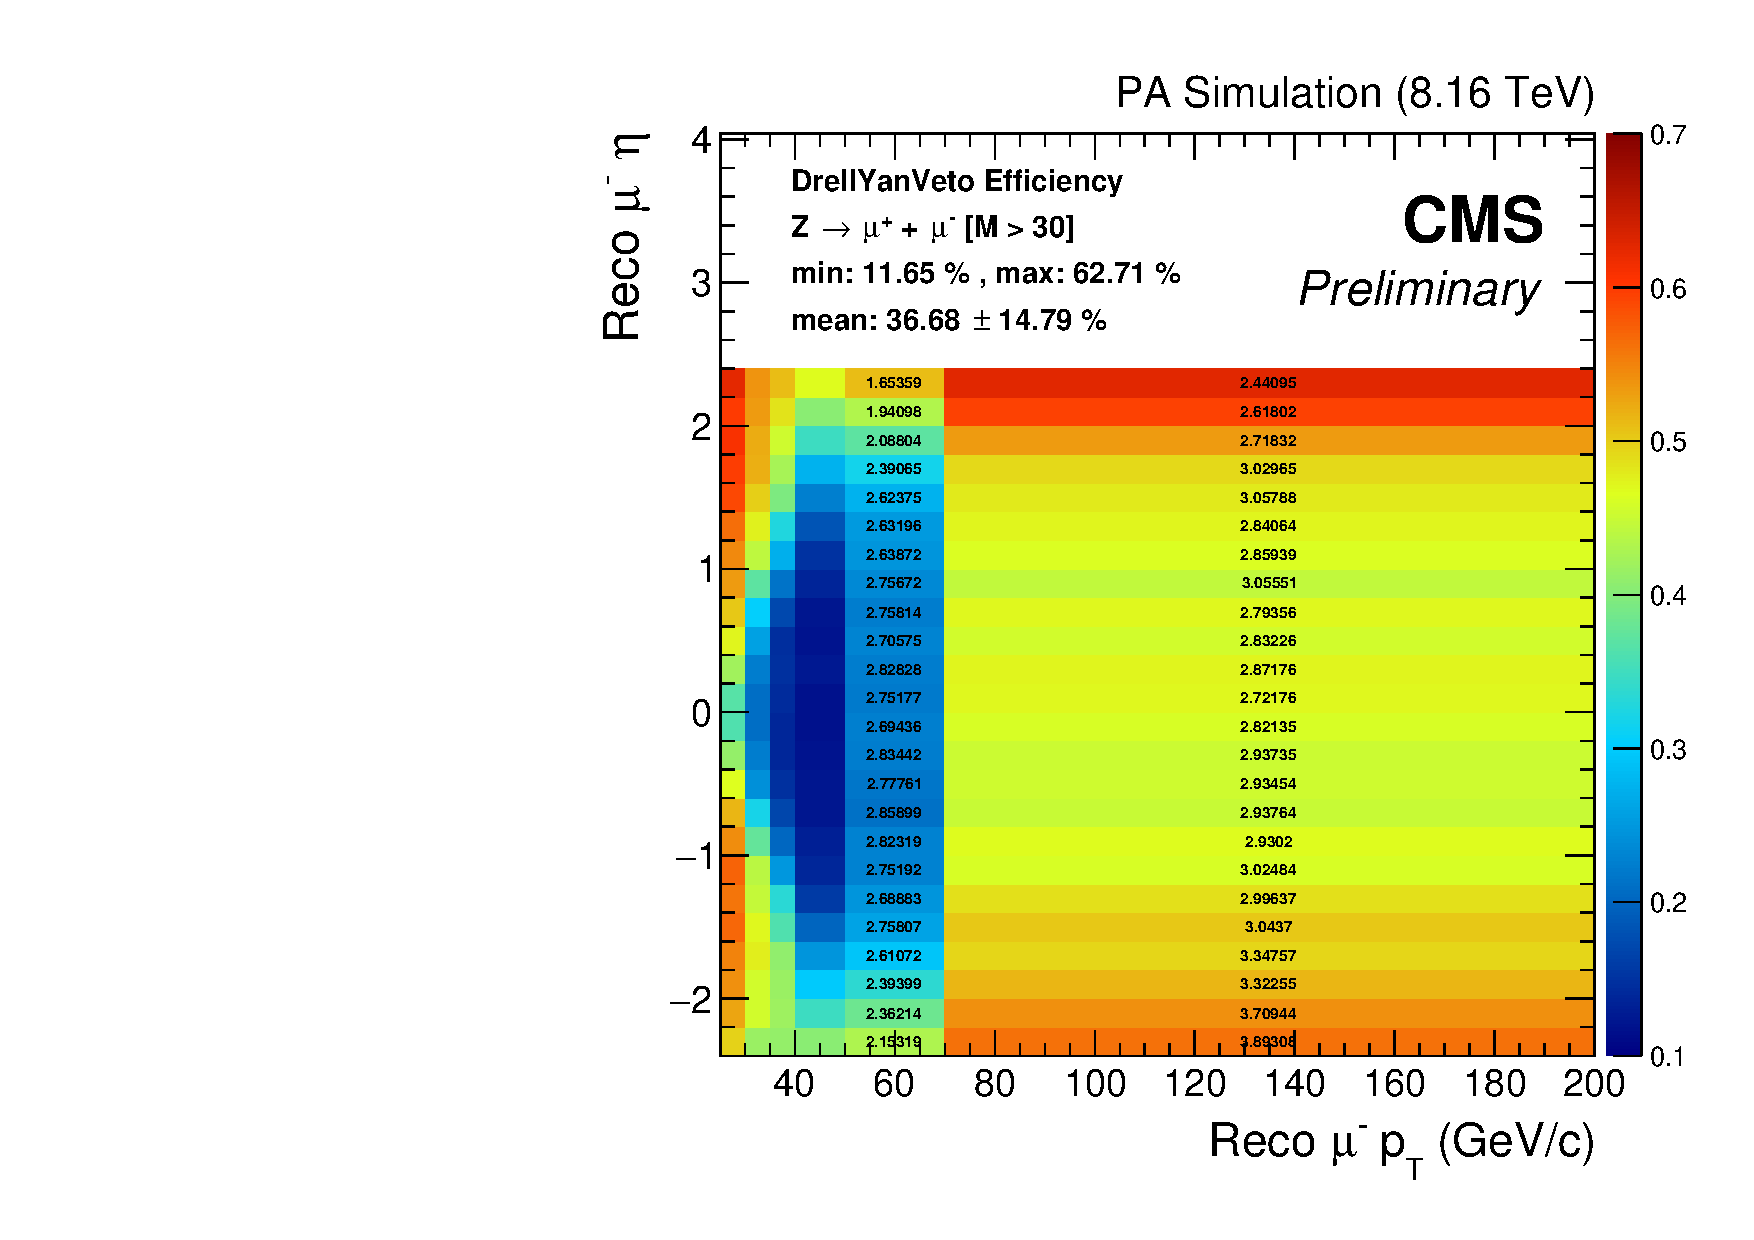
\includegraphics[width=0.45\textwidth]{Figures/WBoson/Analysis/Muon/Efficiency/Efficiency2D/Pt_Eta/MC_ZToMuMu_M_30_Inf/PA/pdf/eff2D_Pt_Eta_MC_ZToMuMu_M_30_Inf_PA_Minus_DrellYanVeto}
   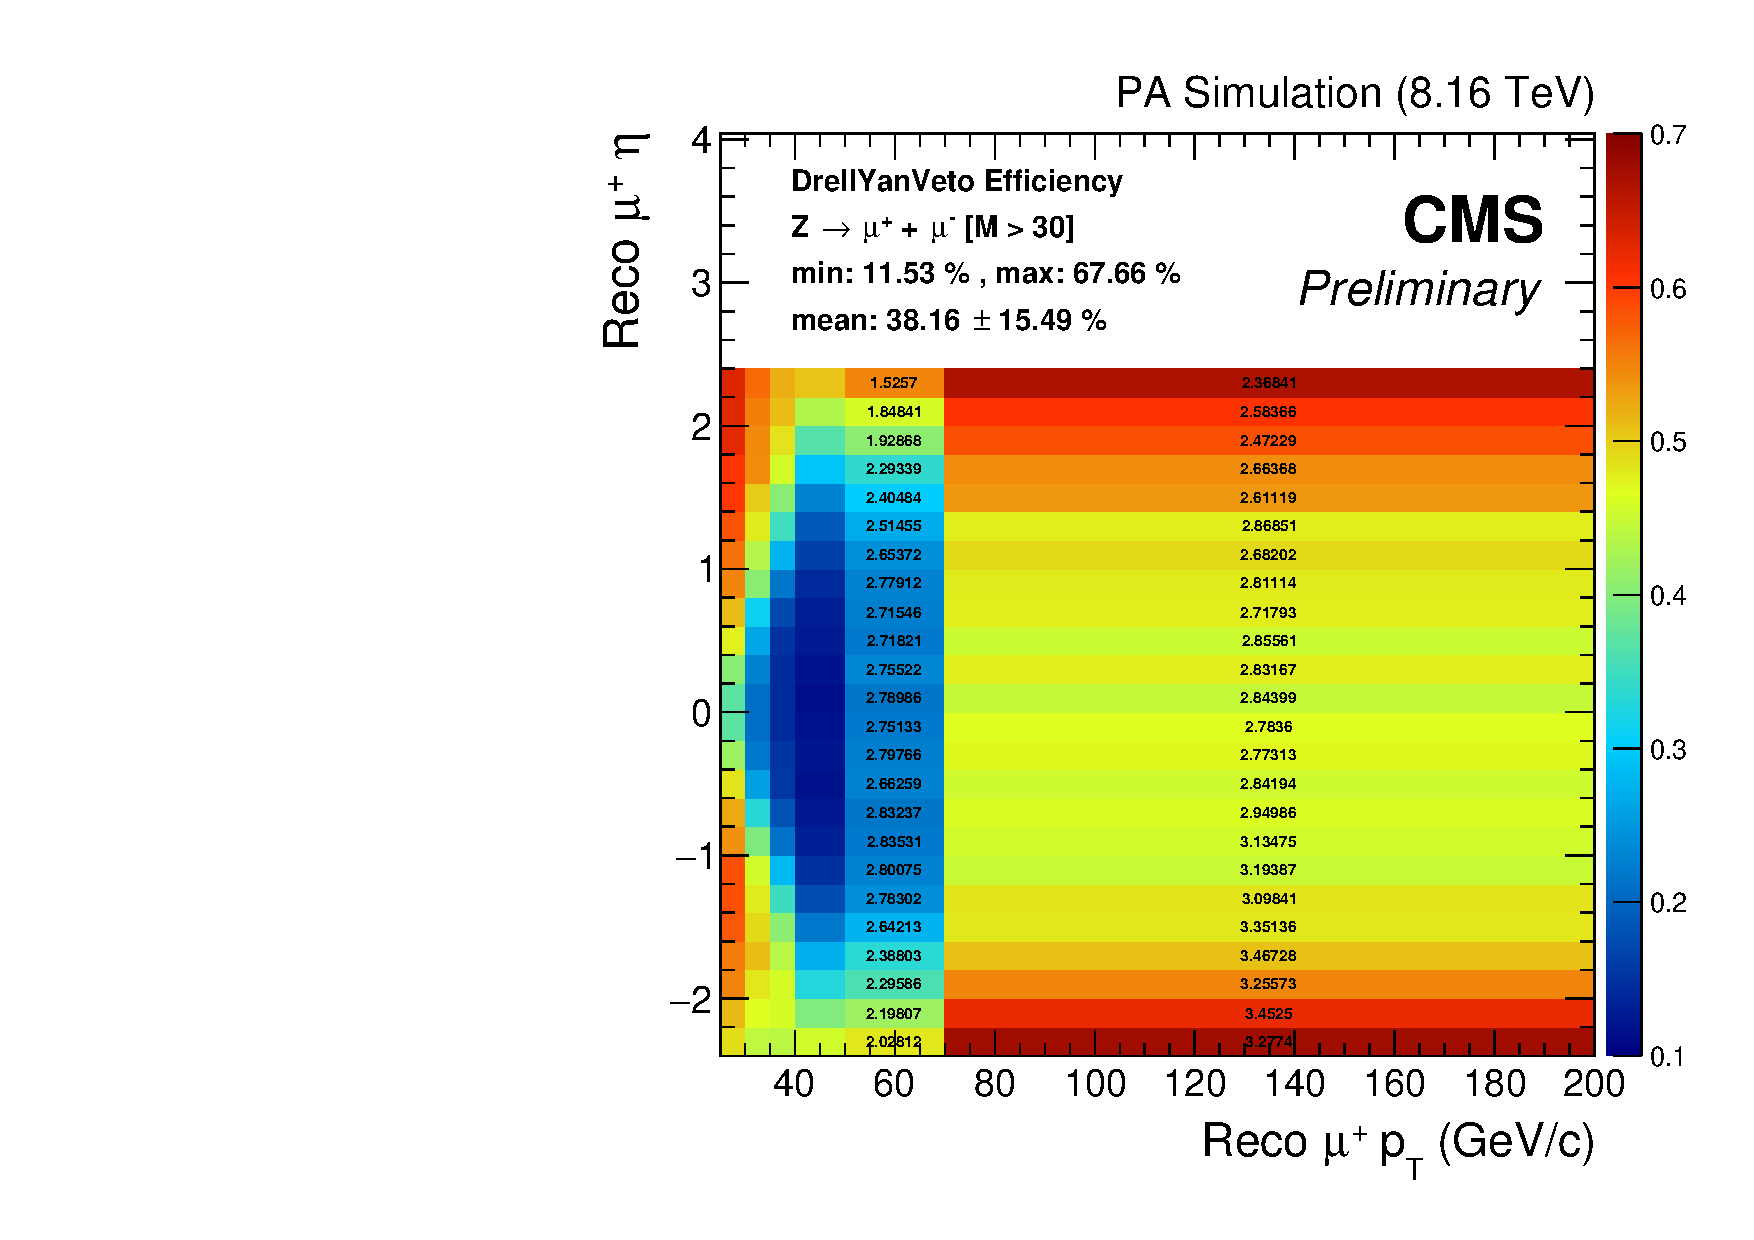
\includegraphics[width=0.45	\textwidth]{Figures/WBoson/Analysis/Muon/Efficiency/Efficiency2D/Pt_Eta/MC_ZToMuMu_M_30_Inf/PA/pdf/eff2D_Pt_Eta_MC_ZToMuMu_M_30_Inf_PA_Plus_DrellYanVeto}
   \caption{Survival probablity of single muons from Drell-Yan ($M > 30$~\GeVcc) MC sample  as a function of the reconstructed muon $\eta$ and \pt, separated in negative (left) and positive (right) charged muons. The \pPb and \Pbp MC samples are combined as described in \sect{sec:WBoson_Sample_CombiningBeamDirection}. The relative statistical efficiency uncertainties scaled by 100 are shown for the two highest \pt bins. Reconstructed muons are required to be within $\pt > 25$~\GeVc and $|\eta| < 2.4$, be trigger matched and pass the isolation and tight selection criteria.}
   \label{fig:DrellYanVetoZEfficiency2D}
 \end{center}
\end{figure}


%%------------------------------------------------------------%%
\subsection{Summary of Event Selection} \label{sec:WBoson_Selection_WSelection}

In summary, the \W candidate selection consists of the detection of a high \pt muon, passing all identification criteria explained in \sect{sec:WBoson_Selection_MuonIdentification}. The leading muon is required to have a $\pt > 25$~\GeVc, and be trigger matched (see \sect{sec:WBoson_Selection_Trigger}). The QCD background is reduced by requiring the leading muon to be isolated. Since high \pt muons can also come from Drell-Yan or resonance decays, a dimuon veto is applied, to remove this potential source of background.

The other signature of a \W event is a high \pt neutrino, estimated through the \ETslash\ . No explicit cut is applied on \ETslash\ . The missing transverse energy is directly used to build templates and extract the yields by fitting the signal and background components. The conditions used to define the signal and background regions of interest are illustrated in \fig{fig:EventSelectionDiagram}.

\begin{figure}[htb]
 \begin{center}
   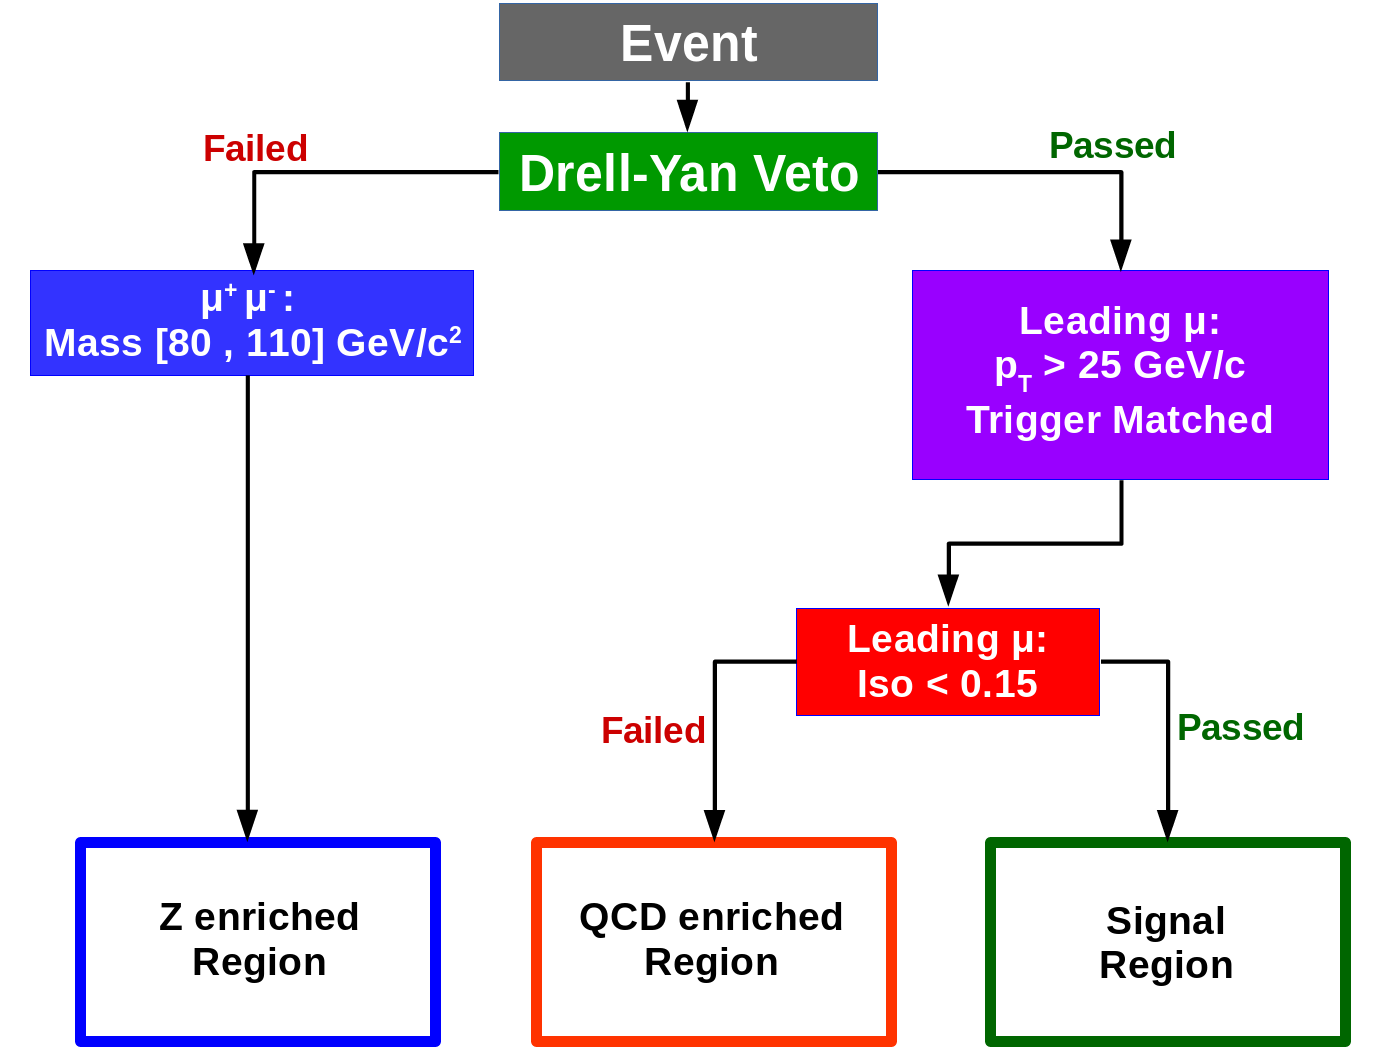
\includegraphics[width=0.9\textwidth]{Figures/WBoson/Analysis/EventSelection/FlowChar.png}
   \caption{Flowchart illustrating the way the events are classified}
   \label{fig:EventSelectionDiagram}
 \end{center}
\end{figure}


% END OF SUBSECTION
\clearpage



\section{Corrections}\label{sec:WBoson_Corrections}


\subsection{Event Activity Reweighing}\label{sec:WBoson_Corrections_EventActivityReweighing}

The \pPb underlying event (UE) activity has been checked in a \DYToMuMu enriched sample of data and MC, by comparing the distribution of the number of tracks and the energy deposited in the Hadron-Forward (HF) calorimeters. The official MC samples embedded in \EPOS minimum bias events are not currently able to reproduce the UE present in \pPb data, as can be observed in \fig{fig:HFrewCheck}.

Since the muon isolation and the MET are computed by summing over particles, they are correlated with the UE. Therefore, any disagreement in the modelling of the event activity can have an impact on the muon efficiency and the signal extraction. The disagreement between the simulation and the data can be caused by the presence of hard probes such as \W bosons, which bias the event activity towards higher multiplicity compared to minimum bias events.

In order to correct the mismodelling of the UE, the simulated distribution of the energy deposited in both sides of the HF calorimeters is reweighed to match the data in a Z enriched region. 
As can be seen in \fig{fig:HFrewCheck}, the HF reweighing significantly improves the MC-data agreement of the MET distribution for \Z boson selected events. 

\begin{figure}[!h]
 \begin{center}
  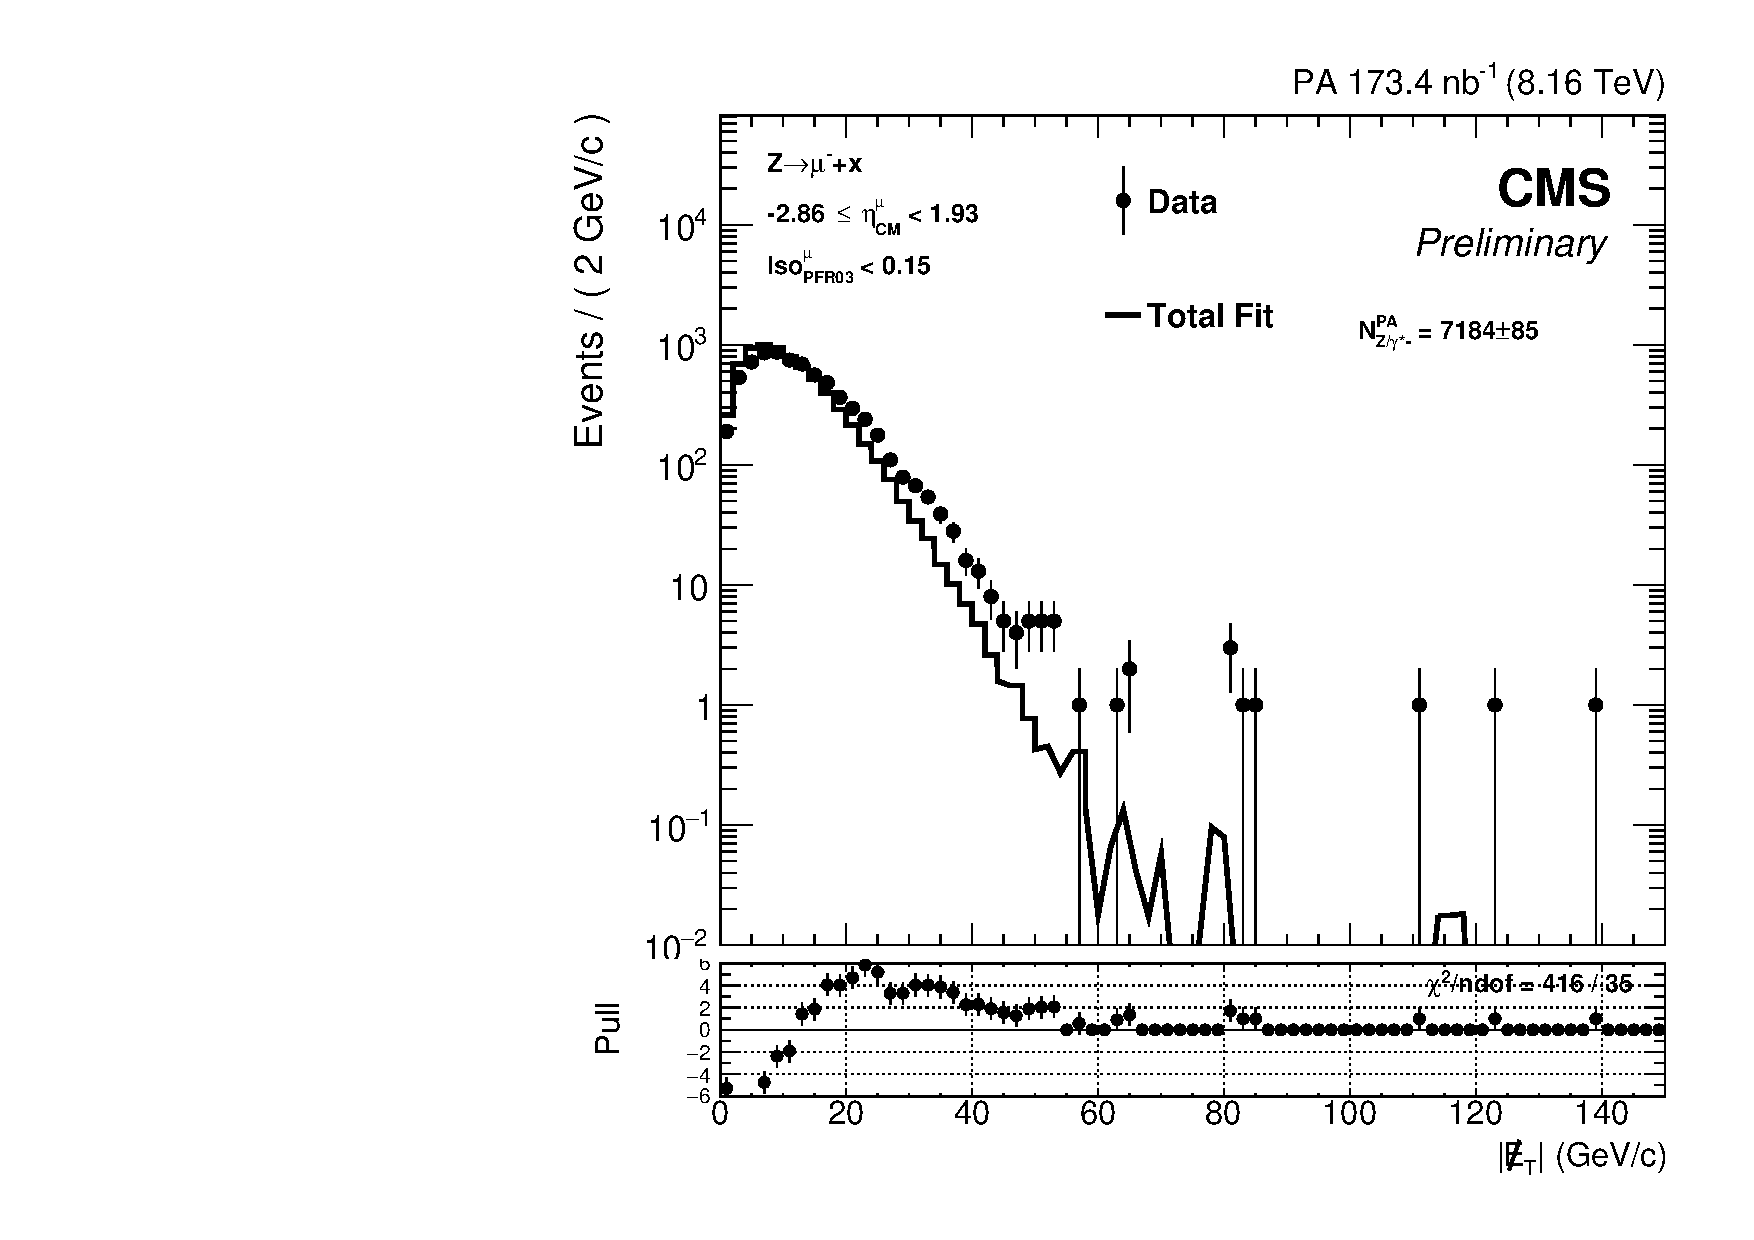
\includegraphics[width=0.4\textwidth]{Figures/WBoson/Analysis/Correction/Recoil/CheckFits/Z/METPF_RAW/PLOT_MET_DATA_ZToMuMi_PA_Model_TEMP_DY_MuEtaCM_m286_193_MuIso_0_15.pdf}
  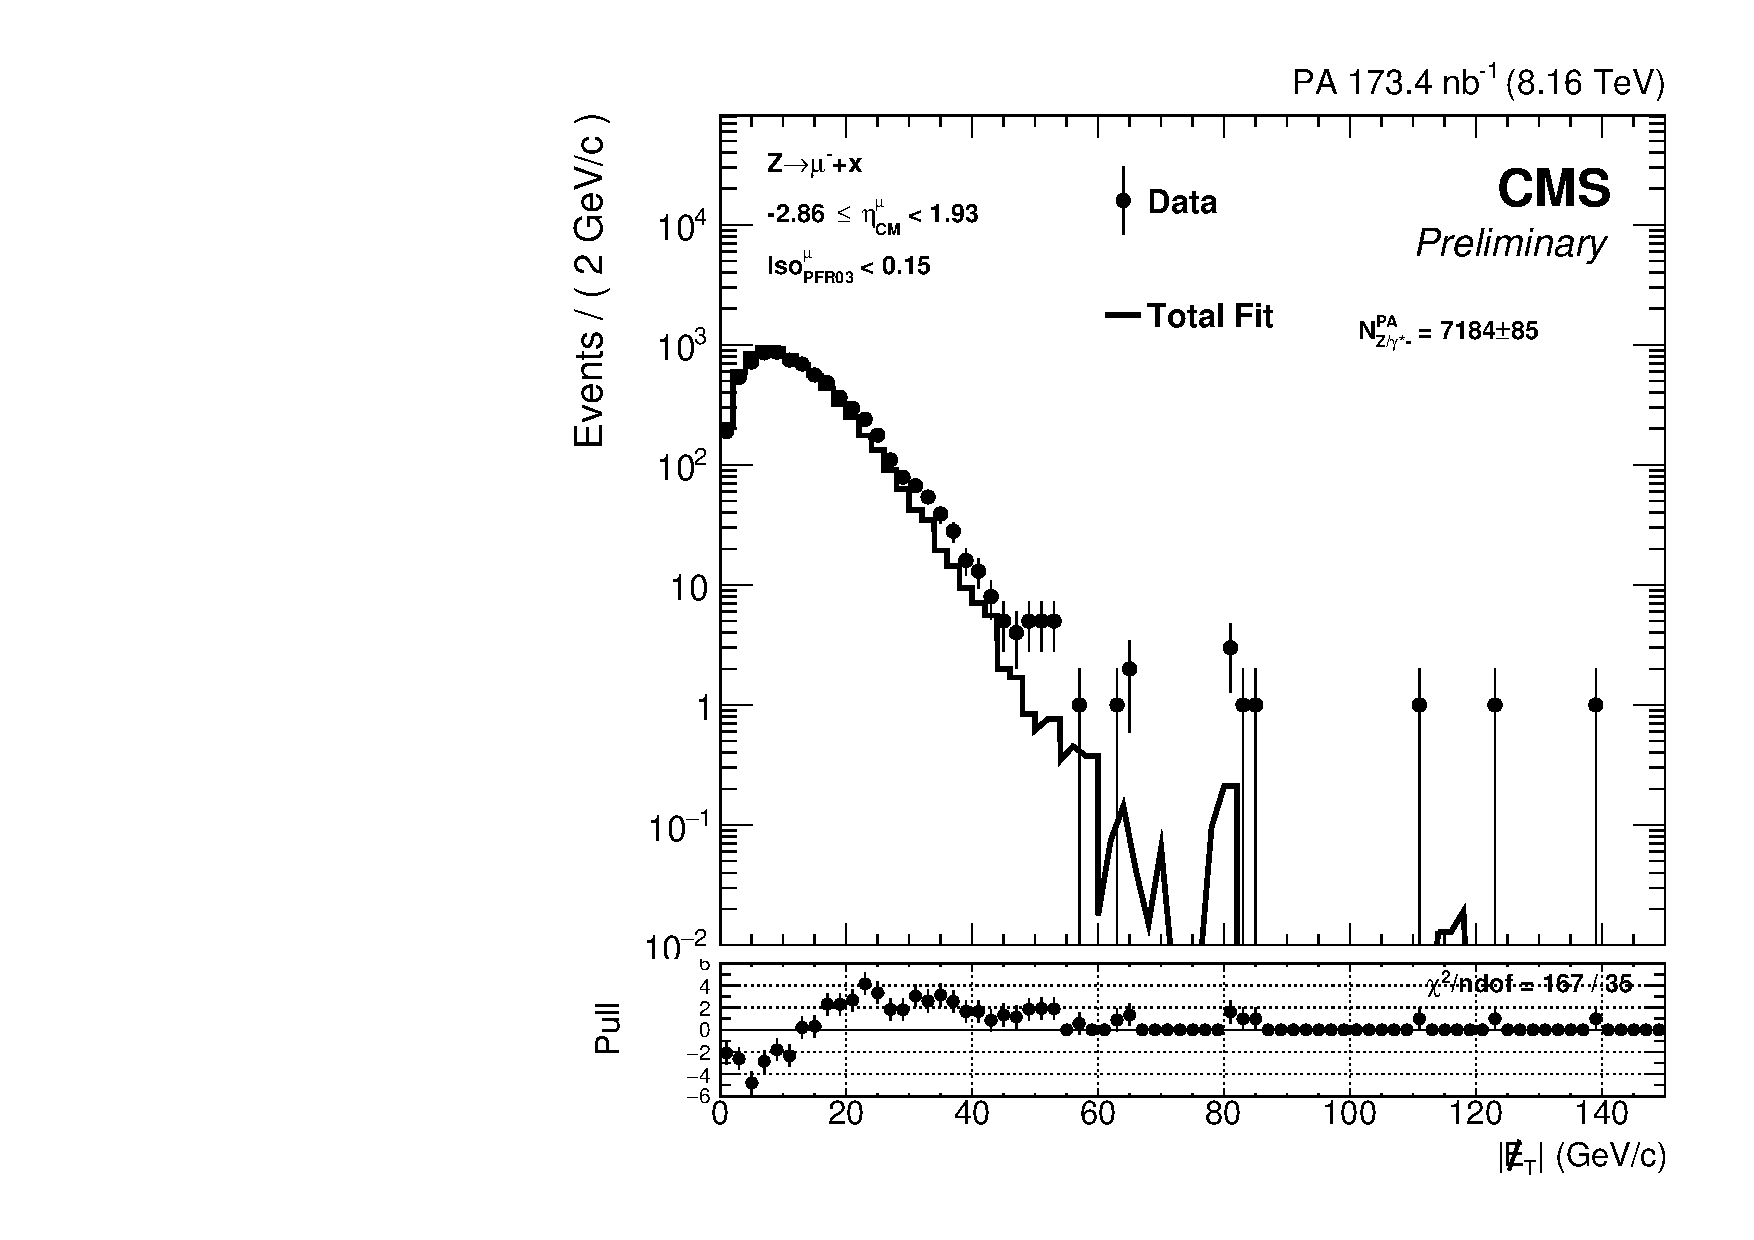
\includegraphics[width=0.4\textwidth]{Figures/WBoson/Analysis/Correction/Recoil/CheckFits/Z/METPF_RAW_HFrew/PLOT_MET_DATA_ZToMuMi_PA_Model_TEMP_DY_MuEtaCM_m286_193_MuIso_0_15.pdf} \\
  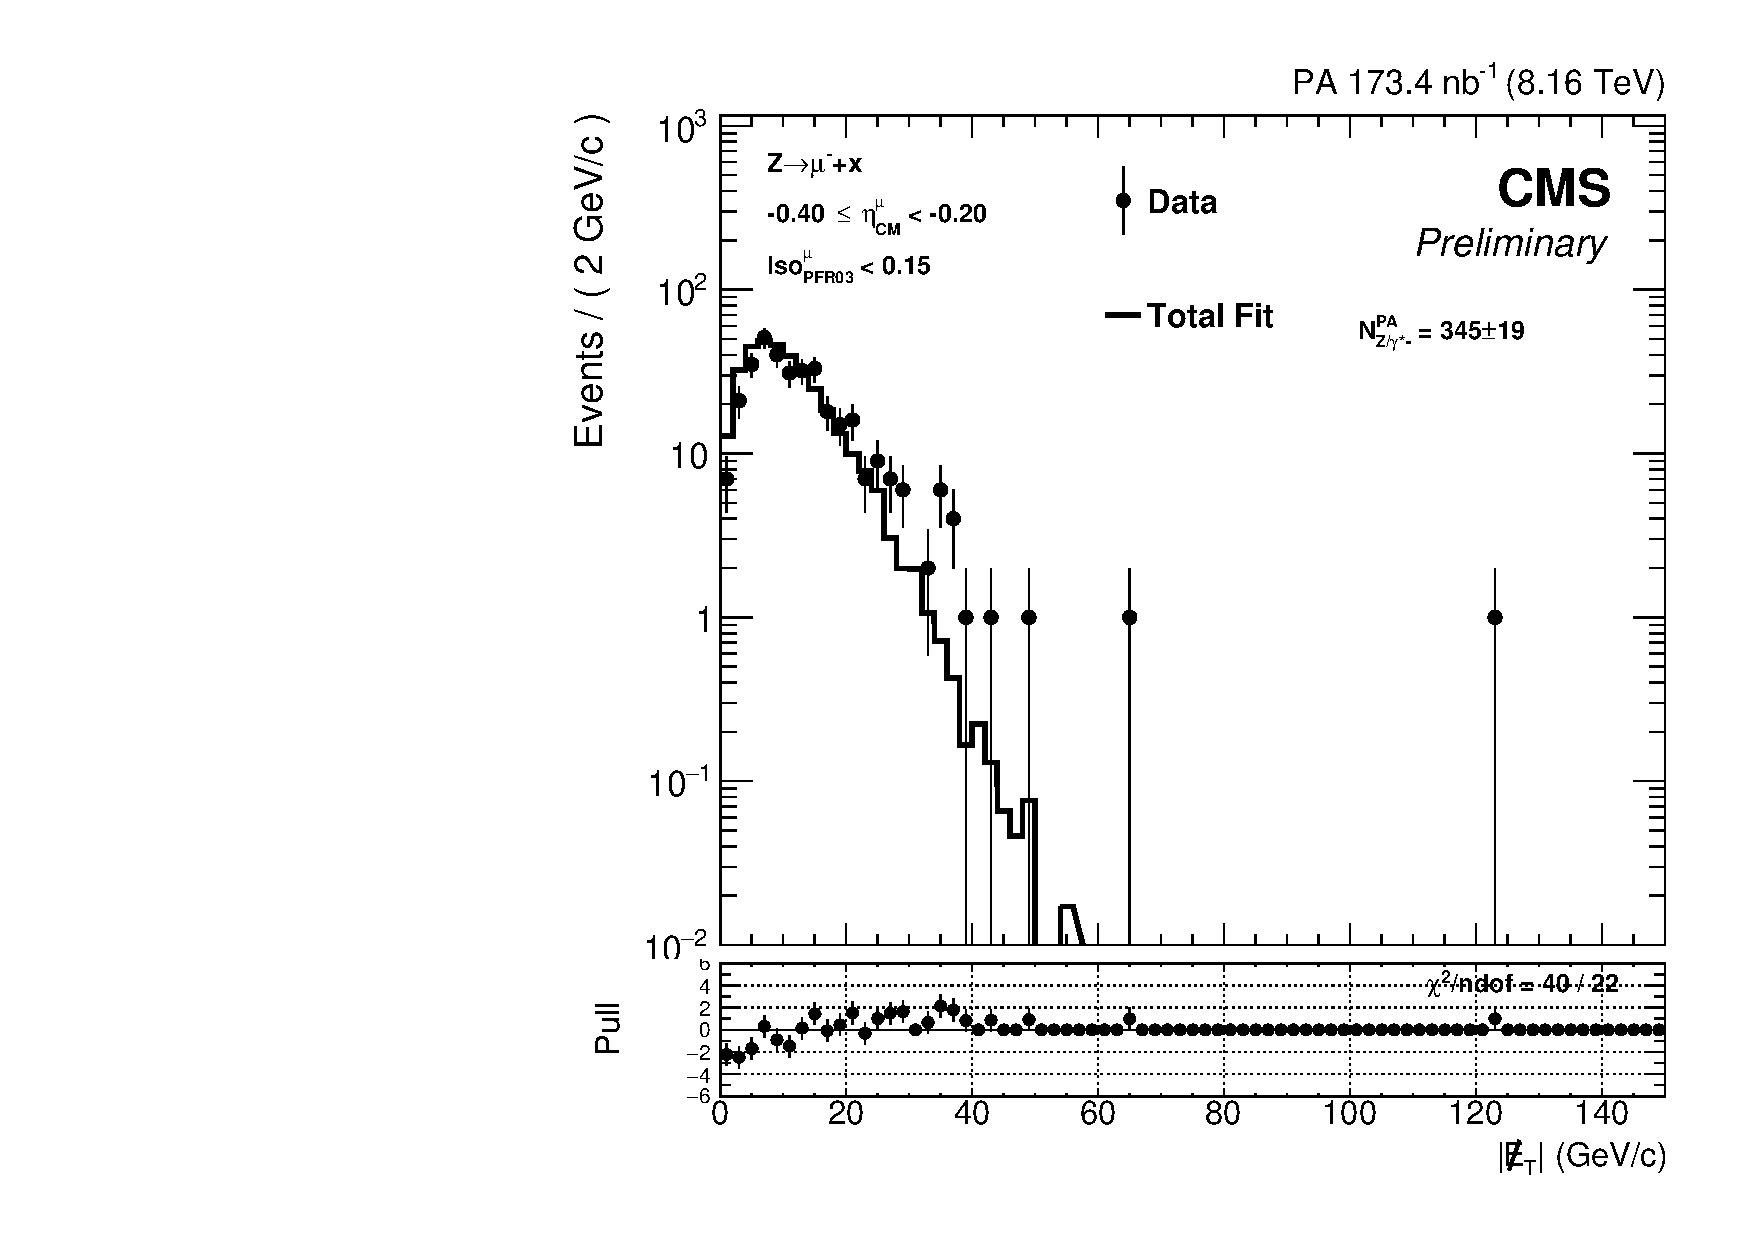
\includegraphics[width=0.4\textwidth]{Figures/WBoson/Analysis/Correction/Recoil/CheckFits/Z/METPF_RAW/PLOT_MET_DATA_ZToMuMi_PA_Model_TEMP_DY_MuEtaCM_m40_m20_MuIso_0_15.pdf}
  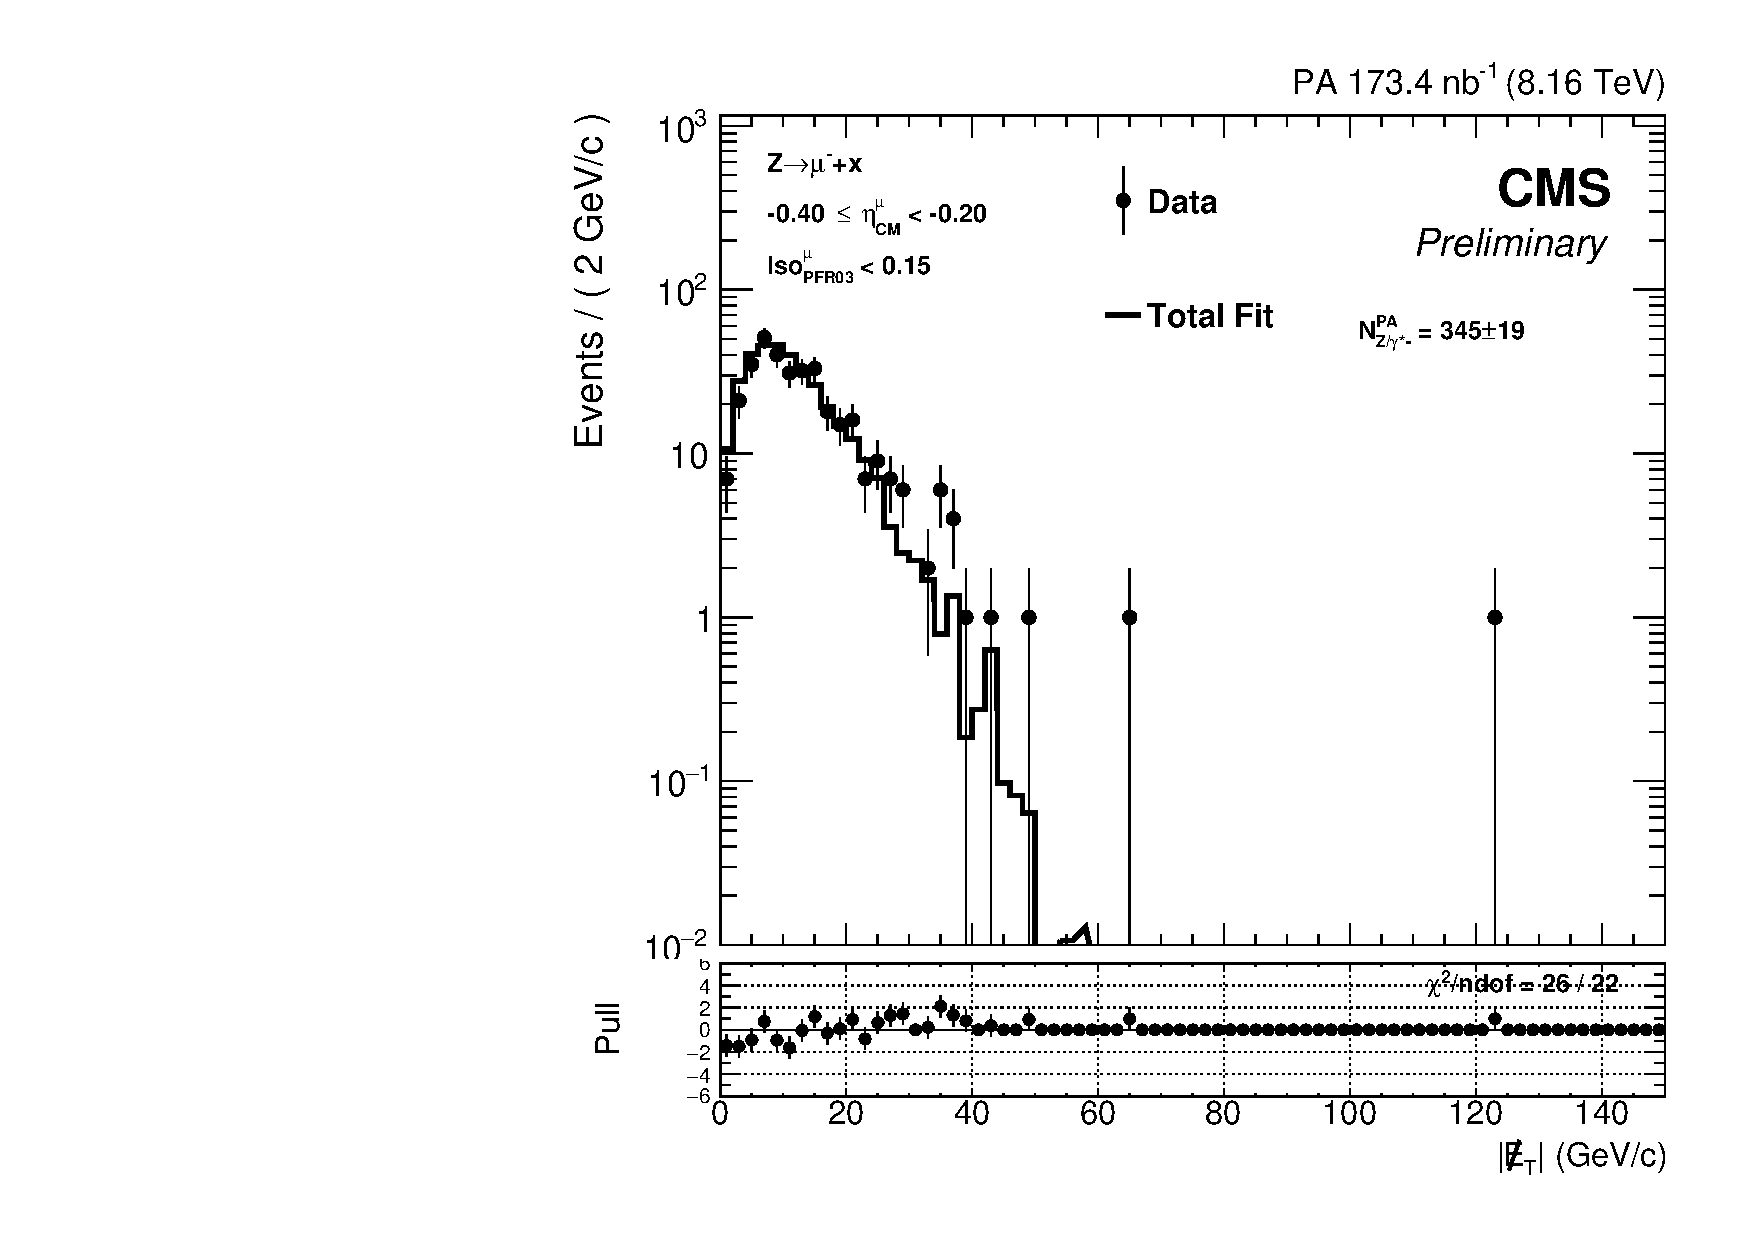
\includegraphics[width=0.4\textwidth]{Figures/WBoson/Analysis/Correction/Recoil/CheckFits/Z/METPF_RAW_HFrew/PLOT_MET_DATA_ZToMuMi_PA_Model_TEMP_DY_MuEtaCM_m40_m20_MuIso_0_15.pdf}
  \caption{A comparison of the MET distribution in data and MC for Z boson selected events. The top plots correspond to the full pseudorapidity range in the analysis while the bottom ones correspond to an specific pseudorapidity bin. The left plots use the PF MET RAW without HF reweighting in MC, while the right ones the MC events are reweighed.}
 \label{fig:HFrewCheck}
 \end{center}
\end{figure}


\subsection{Corrections for MET} \label{sec:WBoson_Corrections_MET}

As mentioned in \sect{sec:WBoson_Selection_MET}, the MET is defined as the sum of the \pt of all the particles reconstructed with the PF algorithm, including those produced by the underlying events. Therefore, the first step to improve the simulation of the MET consist of correcting the modelling of the event activity from the EPOS minimum bias events by reweighing the HF energy distribution as explained in \sect{sec:WBoson_Corrections_EventActivityReweighing}. The low MET region in MC agrees better with the data distribution after applying the HF energy reweighing.

The width of the MET distribution in \ZToMuMu events represents the MET resolution due to the \pt measurement of the PF particles. Differences in the emulation of the detector conditions is one of the main sources of disagreement between simulation and data in the high MET region of a \Z boson enriched sample. The simulated MET resolution describes better the data after correcting the hadronic recoil present in MC events.

\subsection{Definition of recoil} \label{sec:WBoson_Corrections_RecoilCorrection}

The hadronic recoil of \ZToMuMu events is defined as the vector sum of the \pt of all PF candidates excluding the muons from the boson decay. Considering the definition of MET, the recoil vector can be expressed as:

\begin{equation}\label{eq:equT} 
\vec{u}_{T} = -\VETslash\ \ - \vec{q}_{T},
\end{equation}

where $\vec{u}_{T}$ is the hadronic recoil in the transverse plane to the beam direction and $\vec{q}_{T}$ is the transverse momentum of the \Z boson.

In the case of \WToMuNu events, the recoil is defined as:

\begin{equation}\label{eq:equTW}
\vec{u}_{T} = -\VETslash\ \ - \vec{p}_{T}^{\mu},
\end{equation}

where $\vec{p}_{T}^{\mu}$ is the \pt of the muon.

The recoil vector is projected along the transverse plane in the boson direction. The parallel and perpendicular components of the recoil vector with respect to the boson $\vec{q}_{T}$ are labelled as $u_{\parallel}$ and $u_{\perp}$, respectively. \fig{fig:RecoilDefinition} describes the recoil and its components.

\begin{figure}
 \begin{center}
  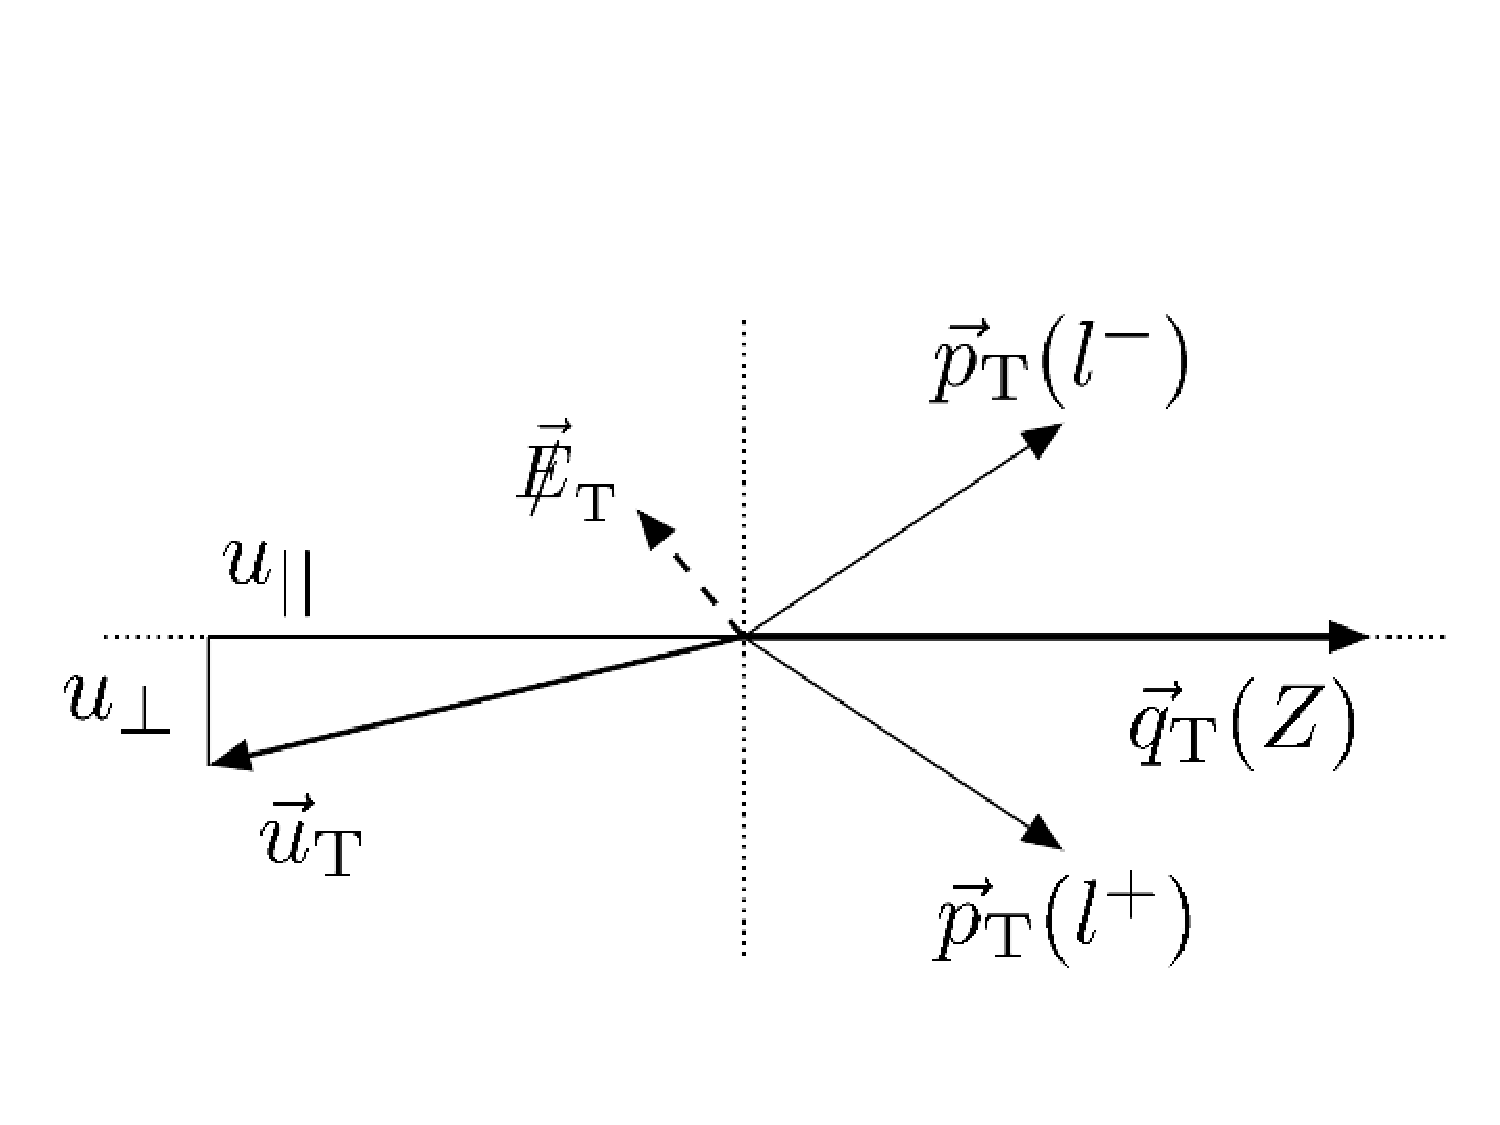
\includegraphics[width=0.4\textwidth]{Figures/WBoson/Analysis/Correction/Recoil/Recoil_Definition.pdf}
  \caption{Definition of the recoil vector and its components for \ZToMuMu events.}
  \label{fig:RecoilDefinition}
 \end{center}
\end{figure}
 
The boson transverse momentum vector $\vec{q}_{T}$ is determined in MC using the reconstructed decay products whenever possible. In the \WToMuNu MC samples, the $\vec{q}_{T}$ is derived from the sum of the \pt of the reconstructed muon and the generated neutrino, while for the \WToTauNu, \DYToTauTau and \ttbar, the $\vec{q}_{T}$ is taken from the generated boson \pt. In the case of \DYToMuMu, if the sub-leading muon falls outside of the coverage of the CMS detector, the \Z boson $q_{T}$ is computed from the sum of the reconstructed leading muon \pt and the generated sub-leading muon \pt, otherwise the $q_{T}$ is equal to the sum of both reconstructed muons \pt.

The recoil corrections are extracted using a \Z control sample. In order to compute them, the parallel and perpendicular components of the recoil vector are determined event by event in data and MC, and their distributions are sorted in bins of $q_{T}$. The recoil distributions are fitted with an unbinned maximum likelihood fit. A combination of two Gaussian functions is chosen to better describe the shape of the recoil distributions. Examples of the distributions of the parallel and perpendicular recoil components, denoted as $u_{1}$ and $u_{2}$ respectively, are shown in \fig{fig:RecoilFits} for data and simulation. Furthermore, the fits performed using the double Gaussian functions, and their corresponding pull distributions are also shown.

\begin{figure}
 \begin{center}
  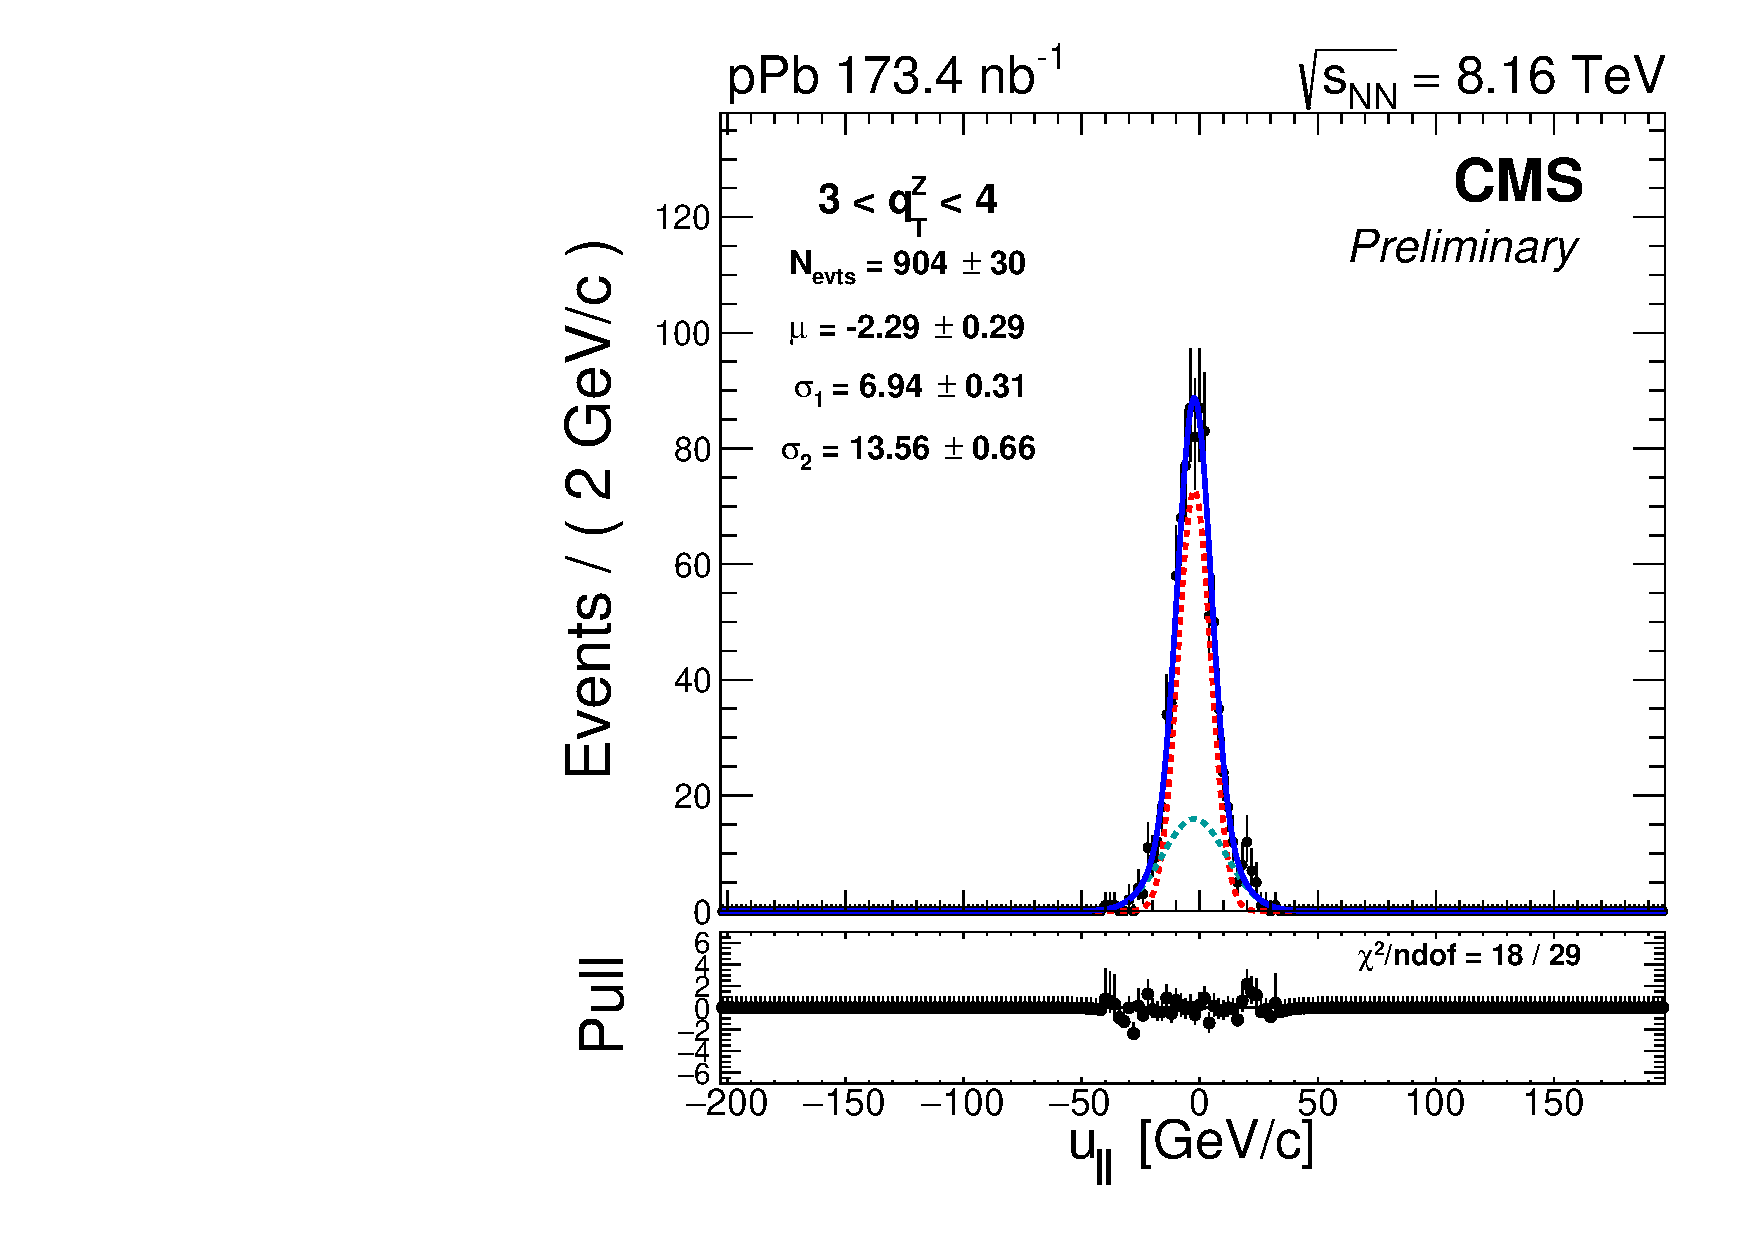
\includegraphics[width=0.4\textwidth]{Figures/WBoson/Analysis/Correction/Recoil/RecoilFits/Data/pfu1fit_2.pdf}
  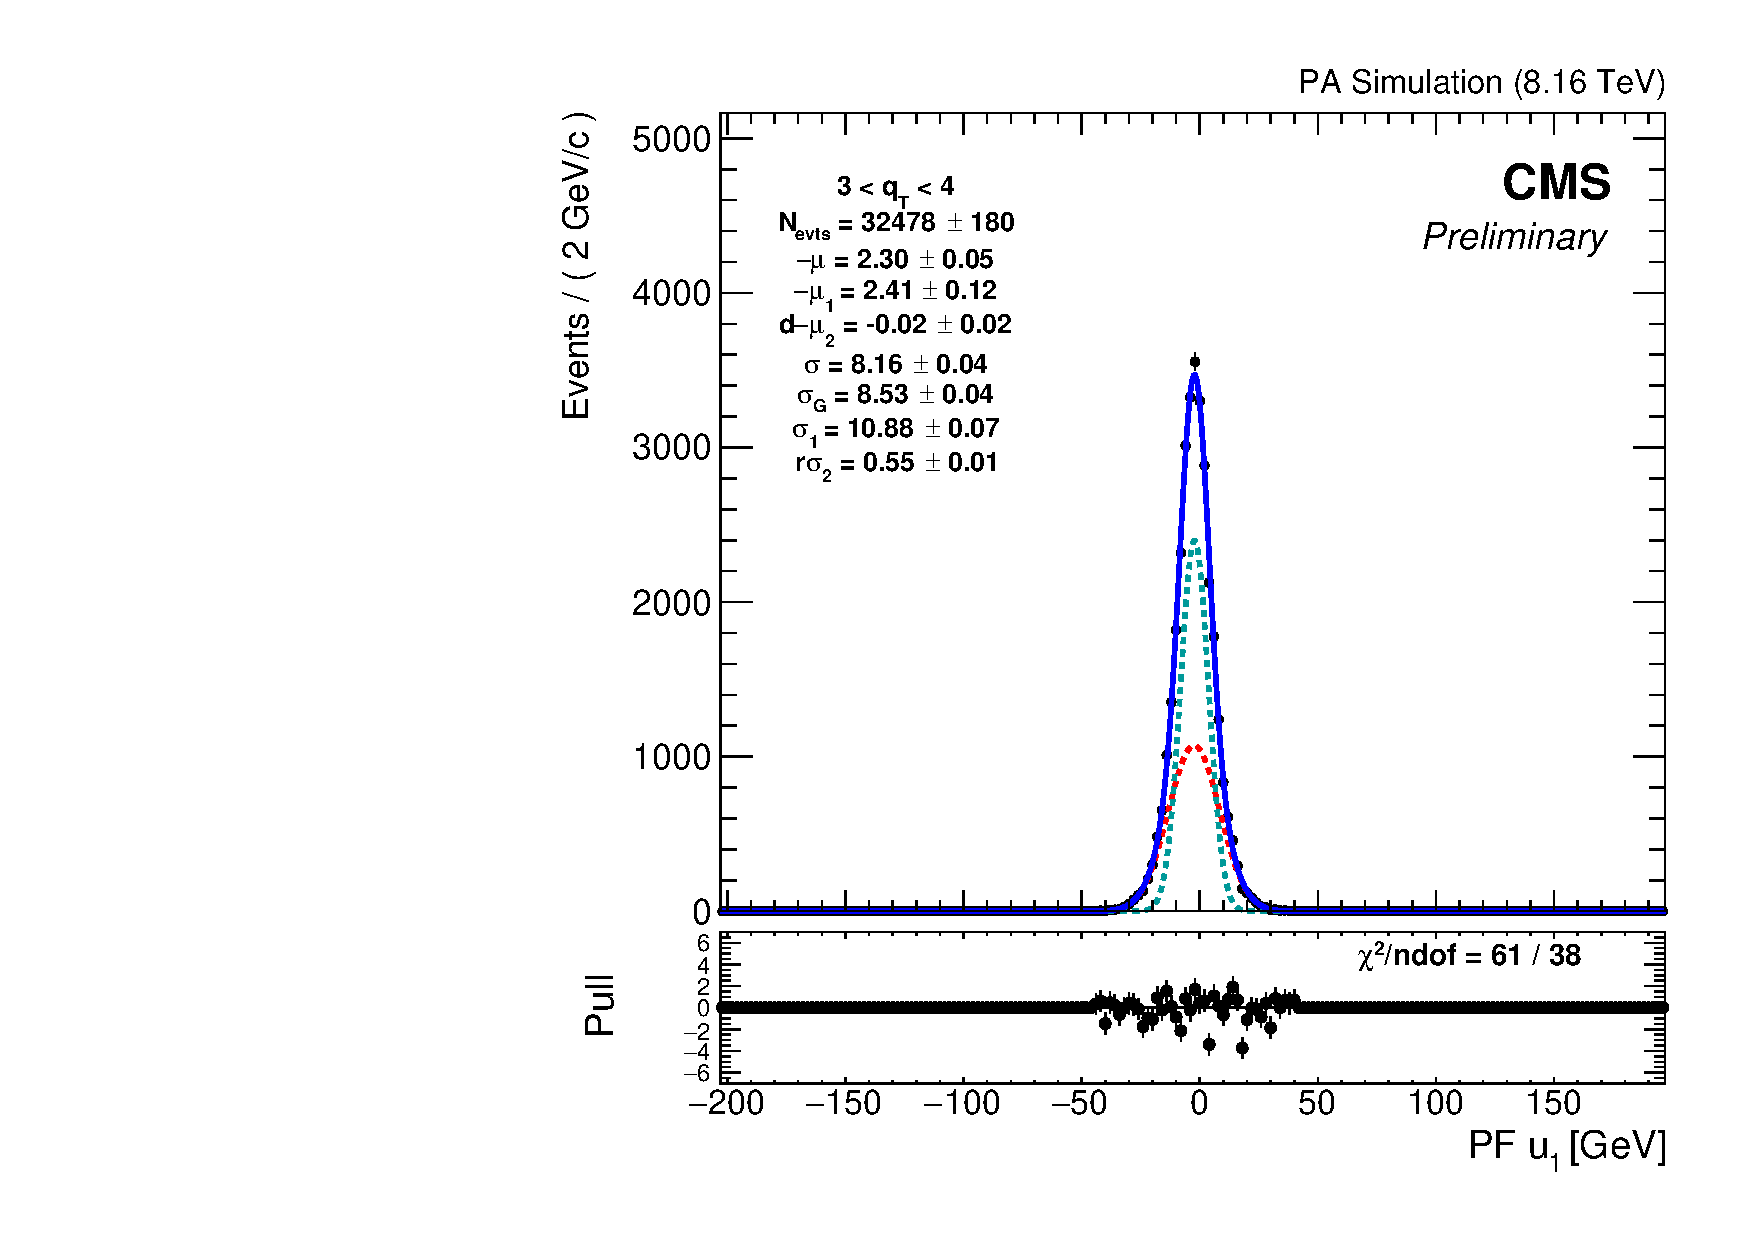
\includegraphics[width=0.4\textwidth]{Figures/WBoson/Analysis/Correction/Recoil/RecoilFits/MC/pfu1fit_2.pdf} \\
  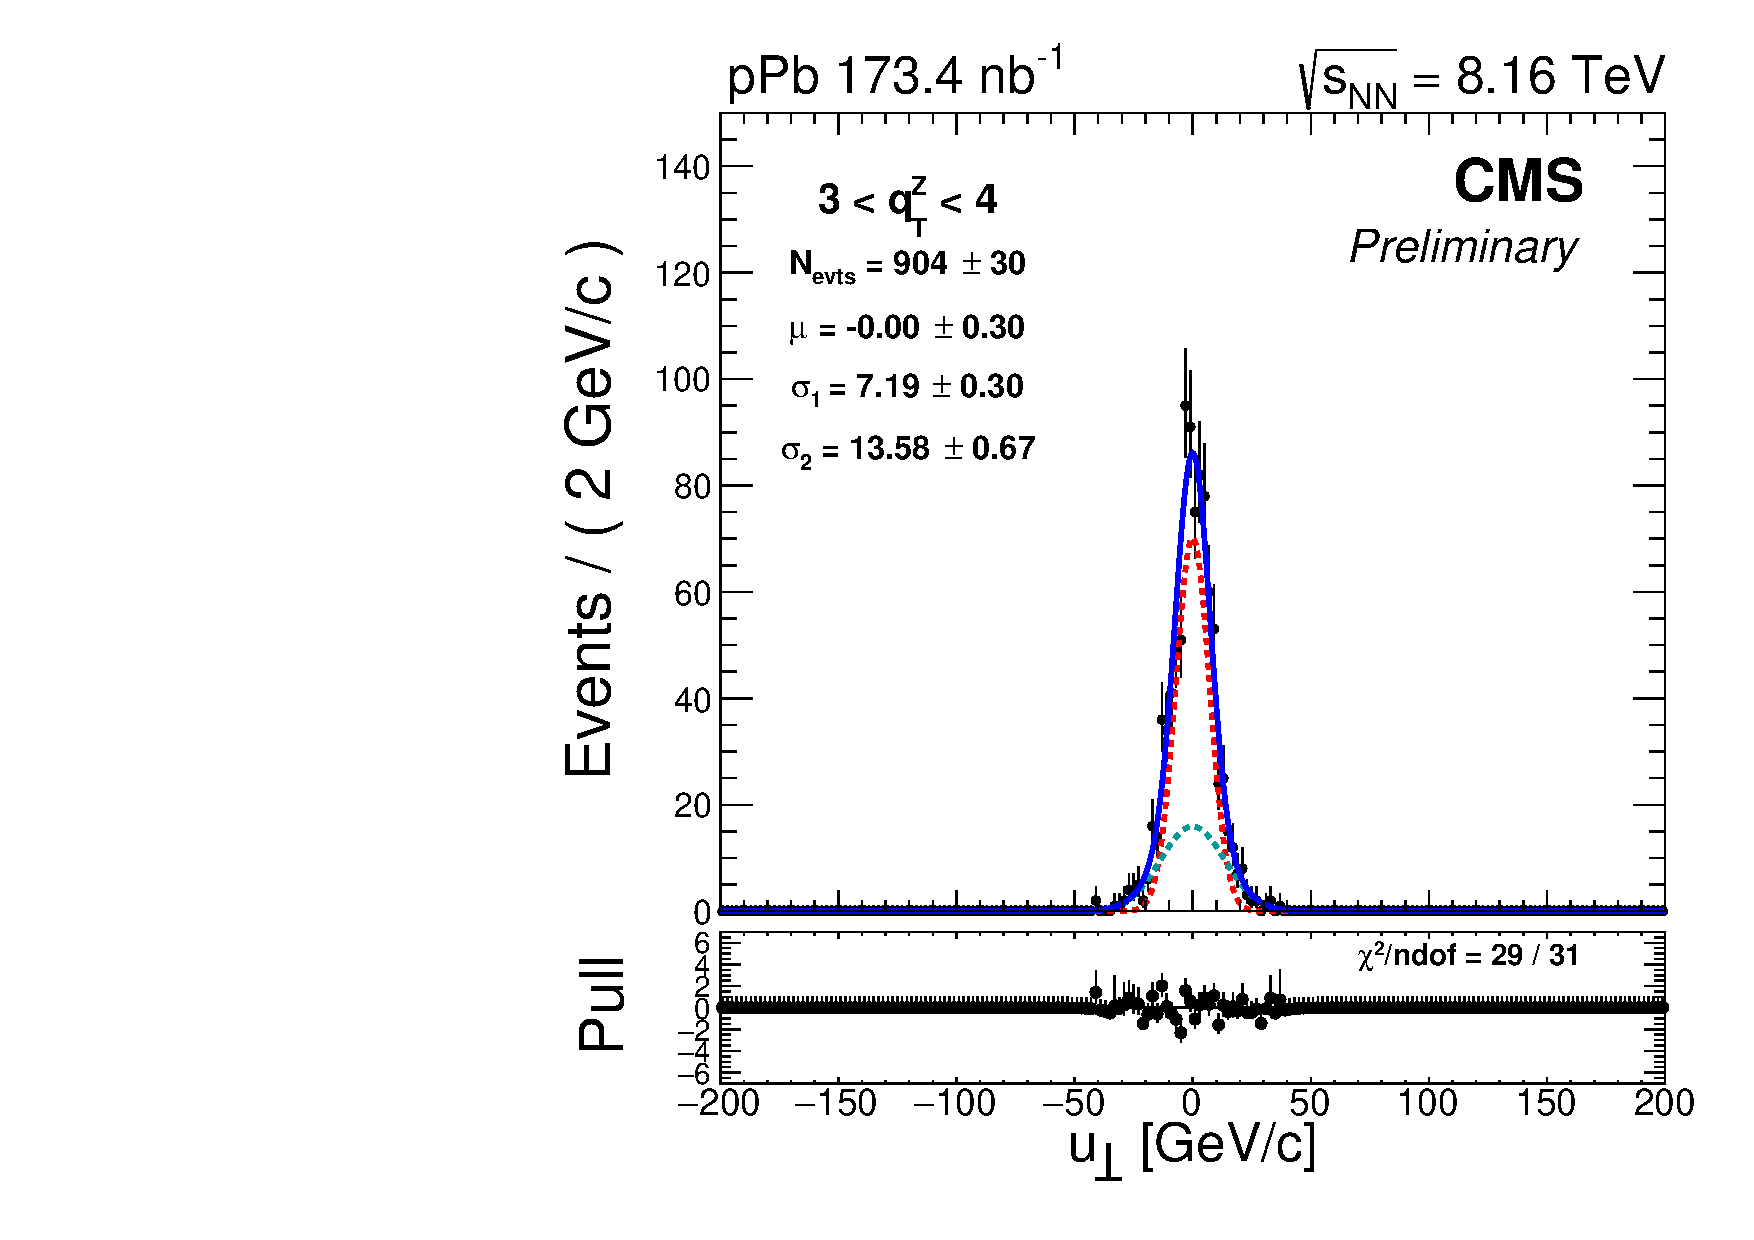
\includegraphics[width=0.4\textwidth]{Figures/WBoson/Analysis/Correction/Recoil/RecoilFits/Data/pfu2fit_2.pdf}
  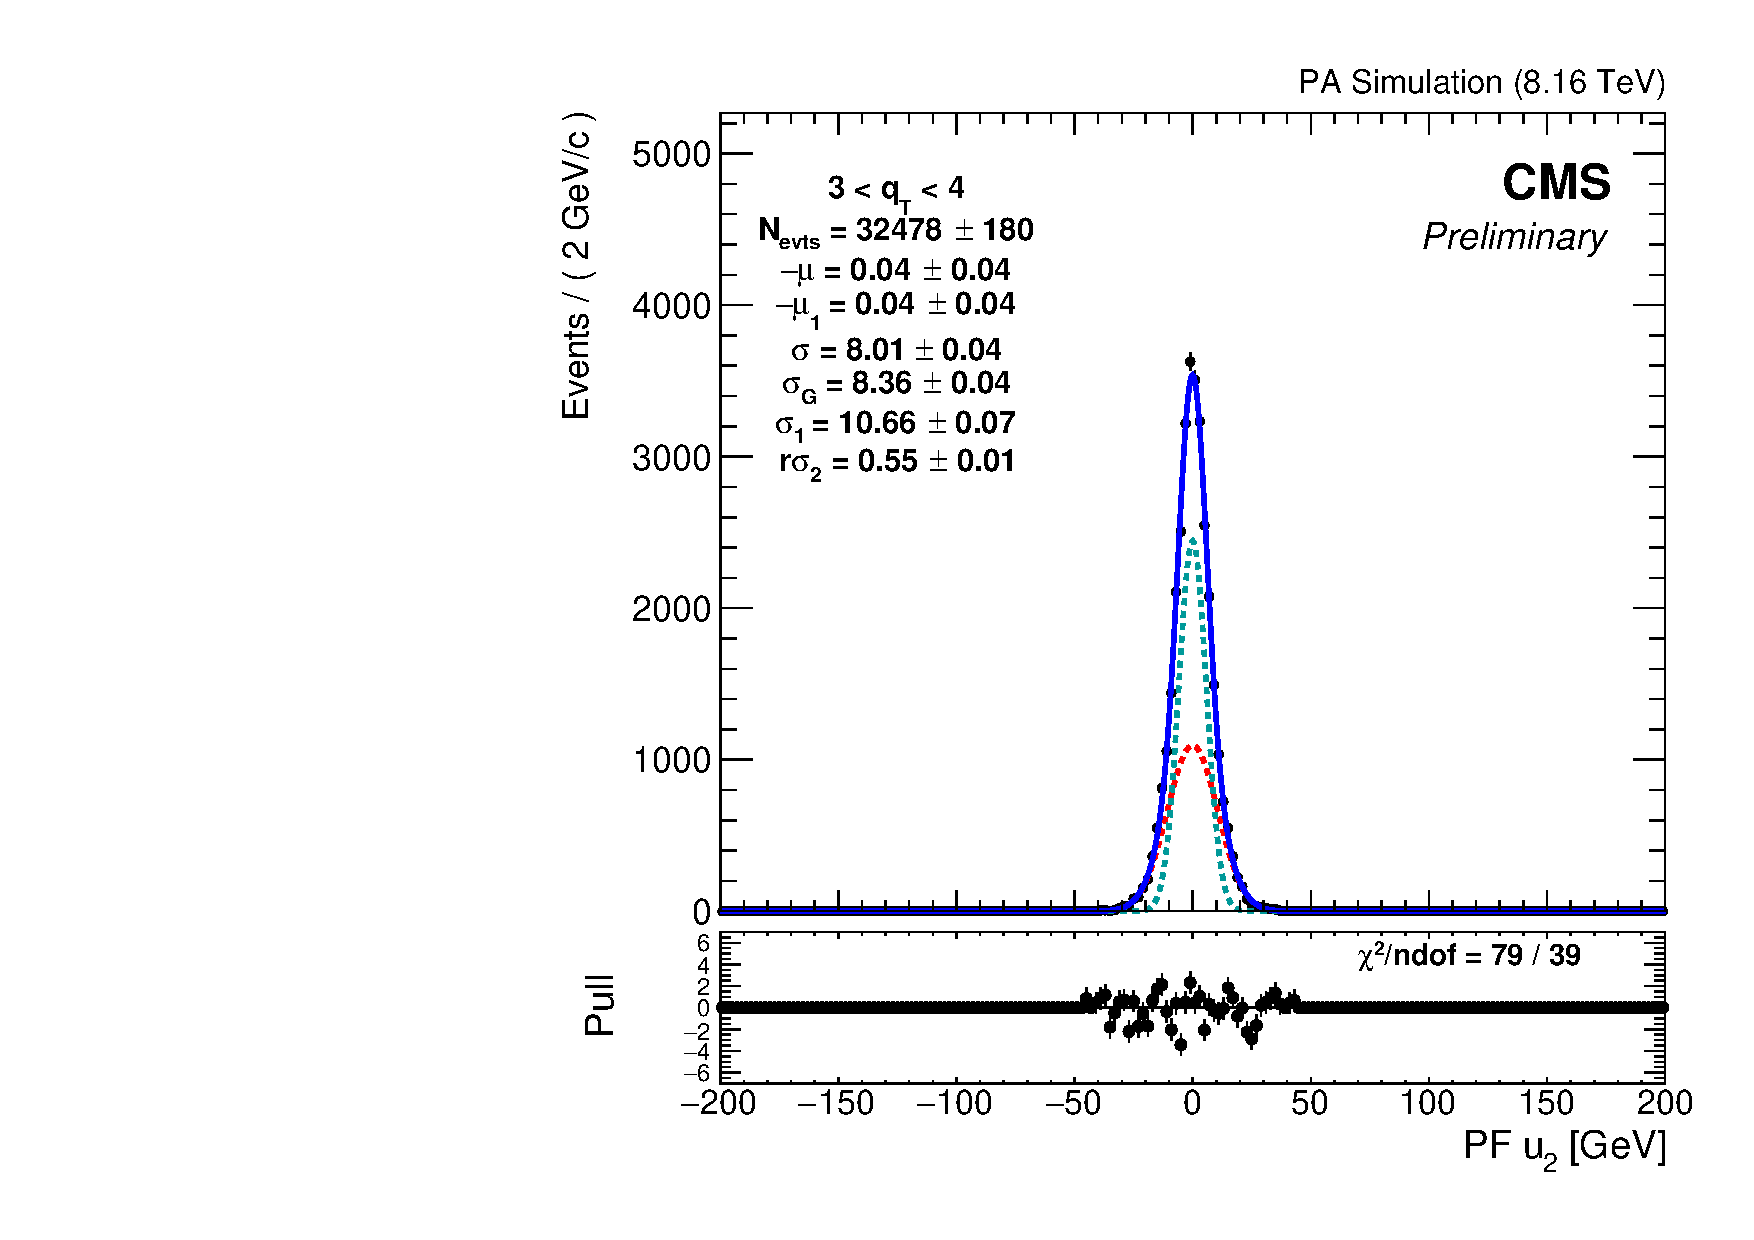
\includegraphics[width=0.4\textwidth]{Figures/WBoson/Analysis/Correction/Recoil/RecoilFits/MC/pfu2fit_2.pdf}
  \caption{Distributions of the parallel (top) and perpendicular (bottom) components of the recoil in data (left) and MC (right). The fit function is based on a weighted sum of two Gaussian distributions. The plots correspond to the $q_{T}$ bin [3, 4]~GeV.}
 \label{fig:RecoilFits}
 \end{center}
\end{figure}
 
\subsubsection{Recoil Scale}\label{sec:WBoson_Corrections_MET_Rscale}

The mean pamareters ($\mu_{1}$ and $\mu_{2}$) of the parallel component of the recoil ($u_{1}$) are extracted in different bins of $q_{T}$ by fitting the recoil distribution as shown in \fig{fig:RecoilFits}. Afterwards, the profile of the average recoil as a function of $q_{T}$ is fitted using the following function: 

\begin{equation}\label{eq:equparparam} 
-\mu_{1,2}(q_{T}) = (c_{0} + c_{1}q_{T})(1 + erf(\alpha q_{T}^{\beta}))
\end{equation}

The fits of the average values of the parallel component of the recoil versus $q_{T}$ are shown in \fig{fig:figU1RecoilScaleFit}. In addition, the average mean value given by $\mu = f \cdot \mu_{1} + (1 - f) \cdot \mu_{2}$, is also shown. The difference between data and the simulation as a function of $q_{T}$ is used on an event by event basis to correct the scale of the recoil in MC.

\begin{figure}
 \begin{center}
  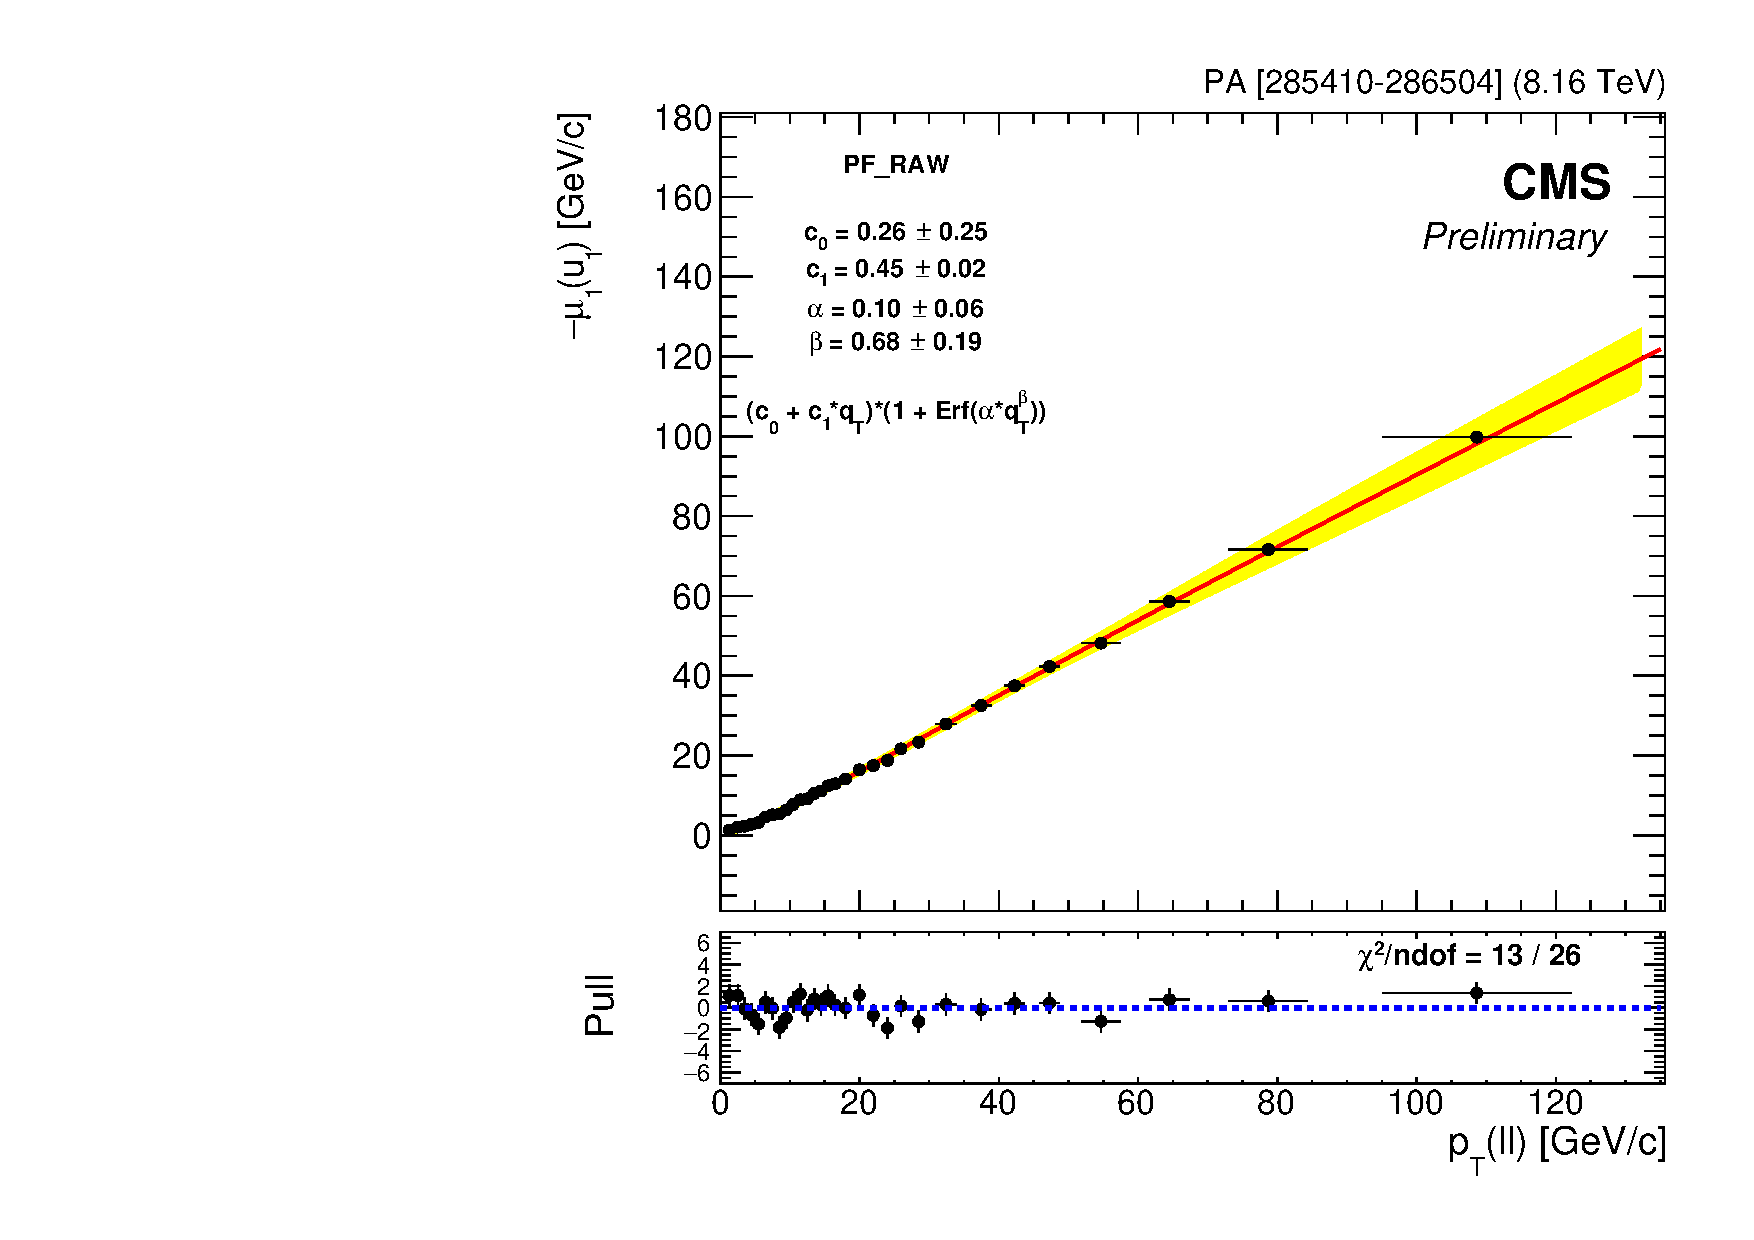
\includegraphics[width=0.3\textwidth]{Figures/WBoson/Analysis/Correction/Recoil/RecoilFitsqT/Data/fitPFu1mean1.pdf}
  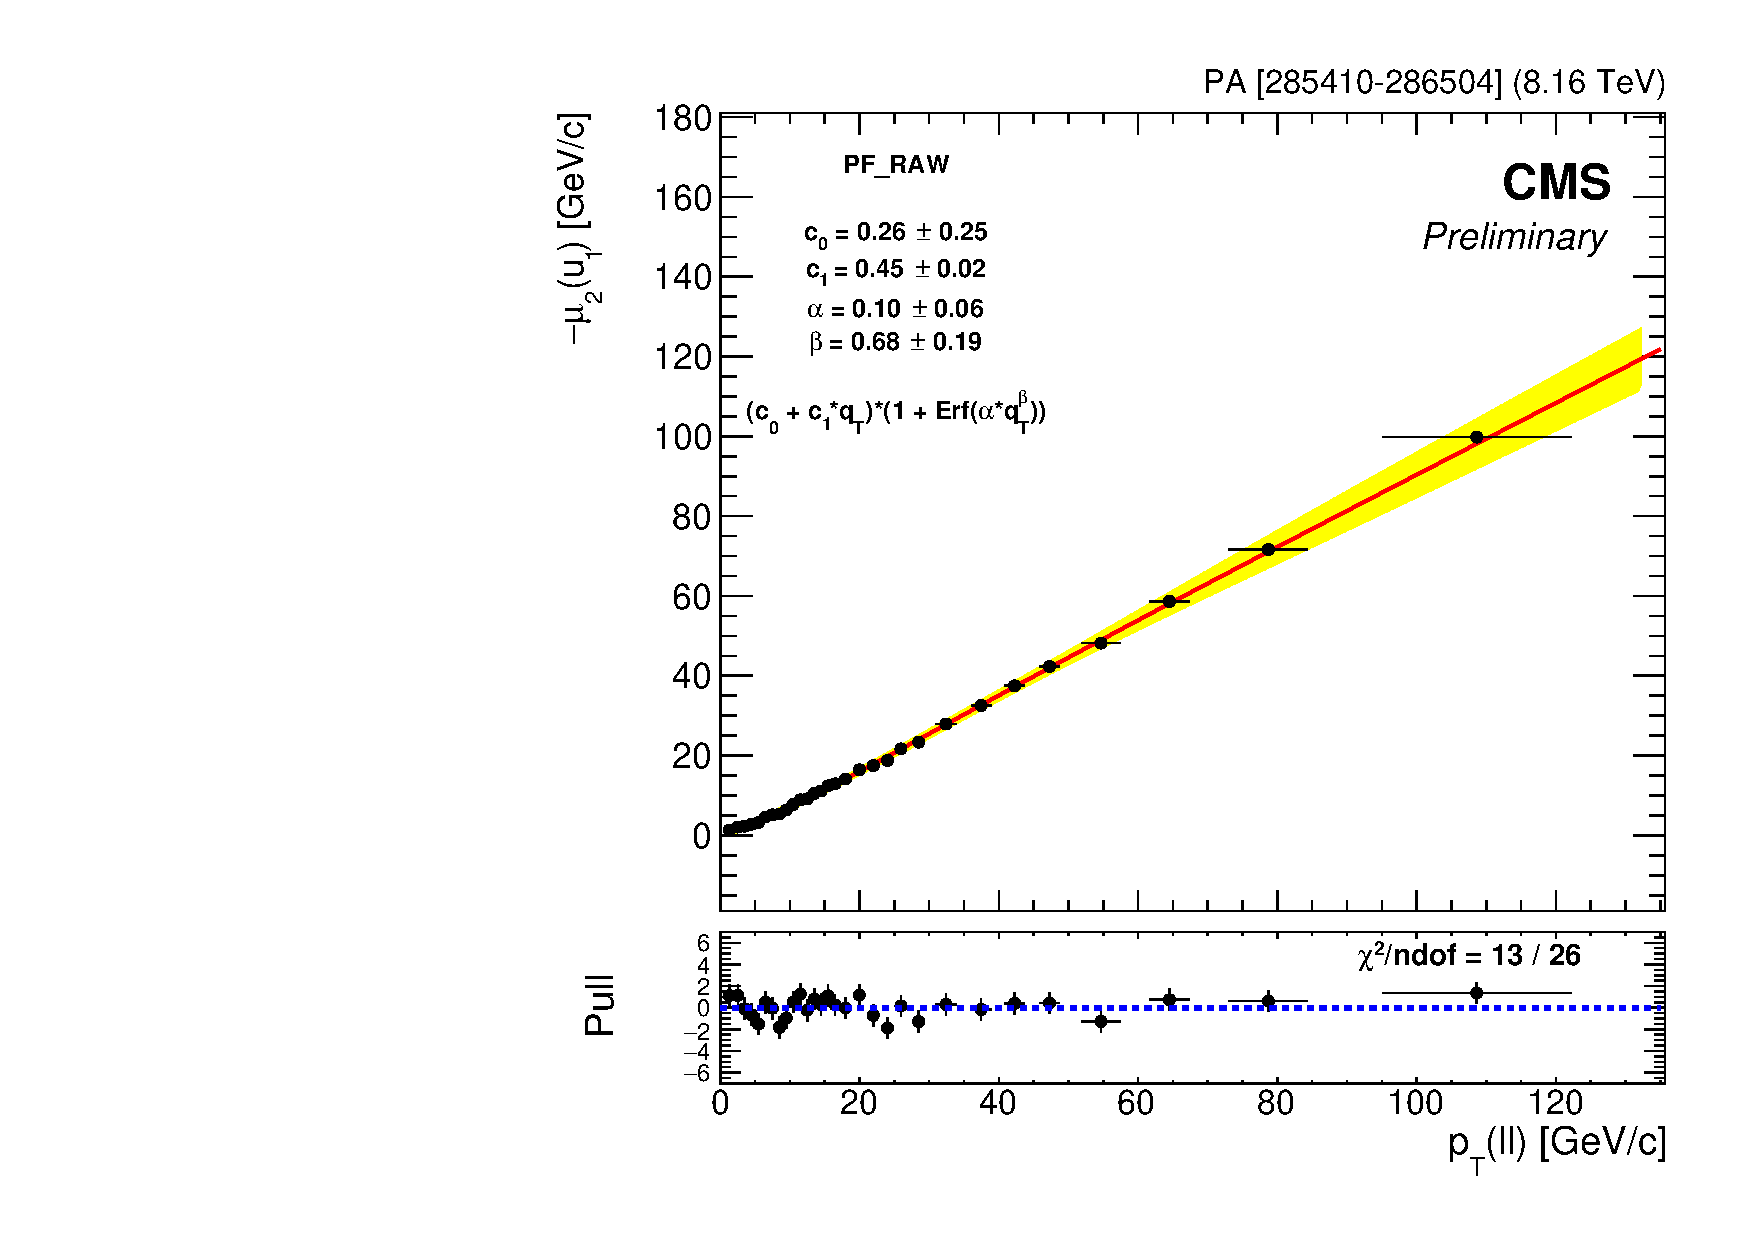
\includegraphics[width=0.3\textwidth]{Figures/WBoson/Analysis/Correction/Recoil/RecoilFitsqT/Data/fitPFu1mean2.pdf}
  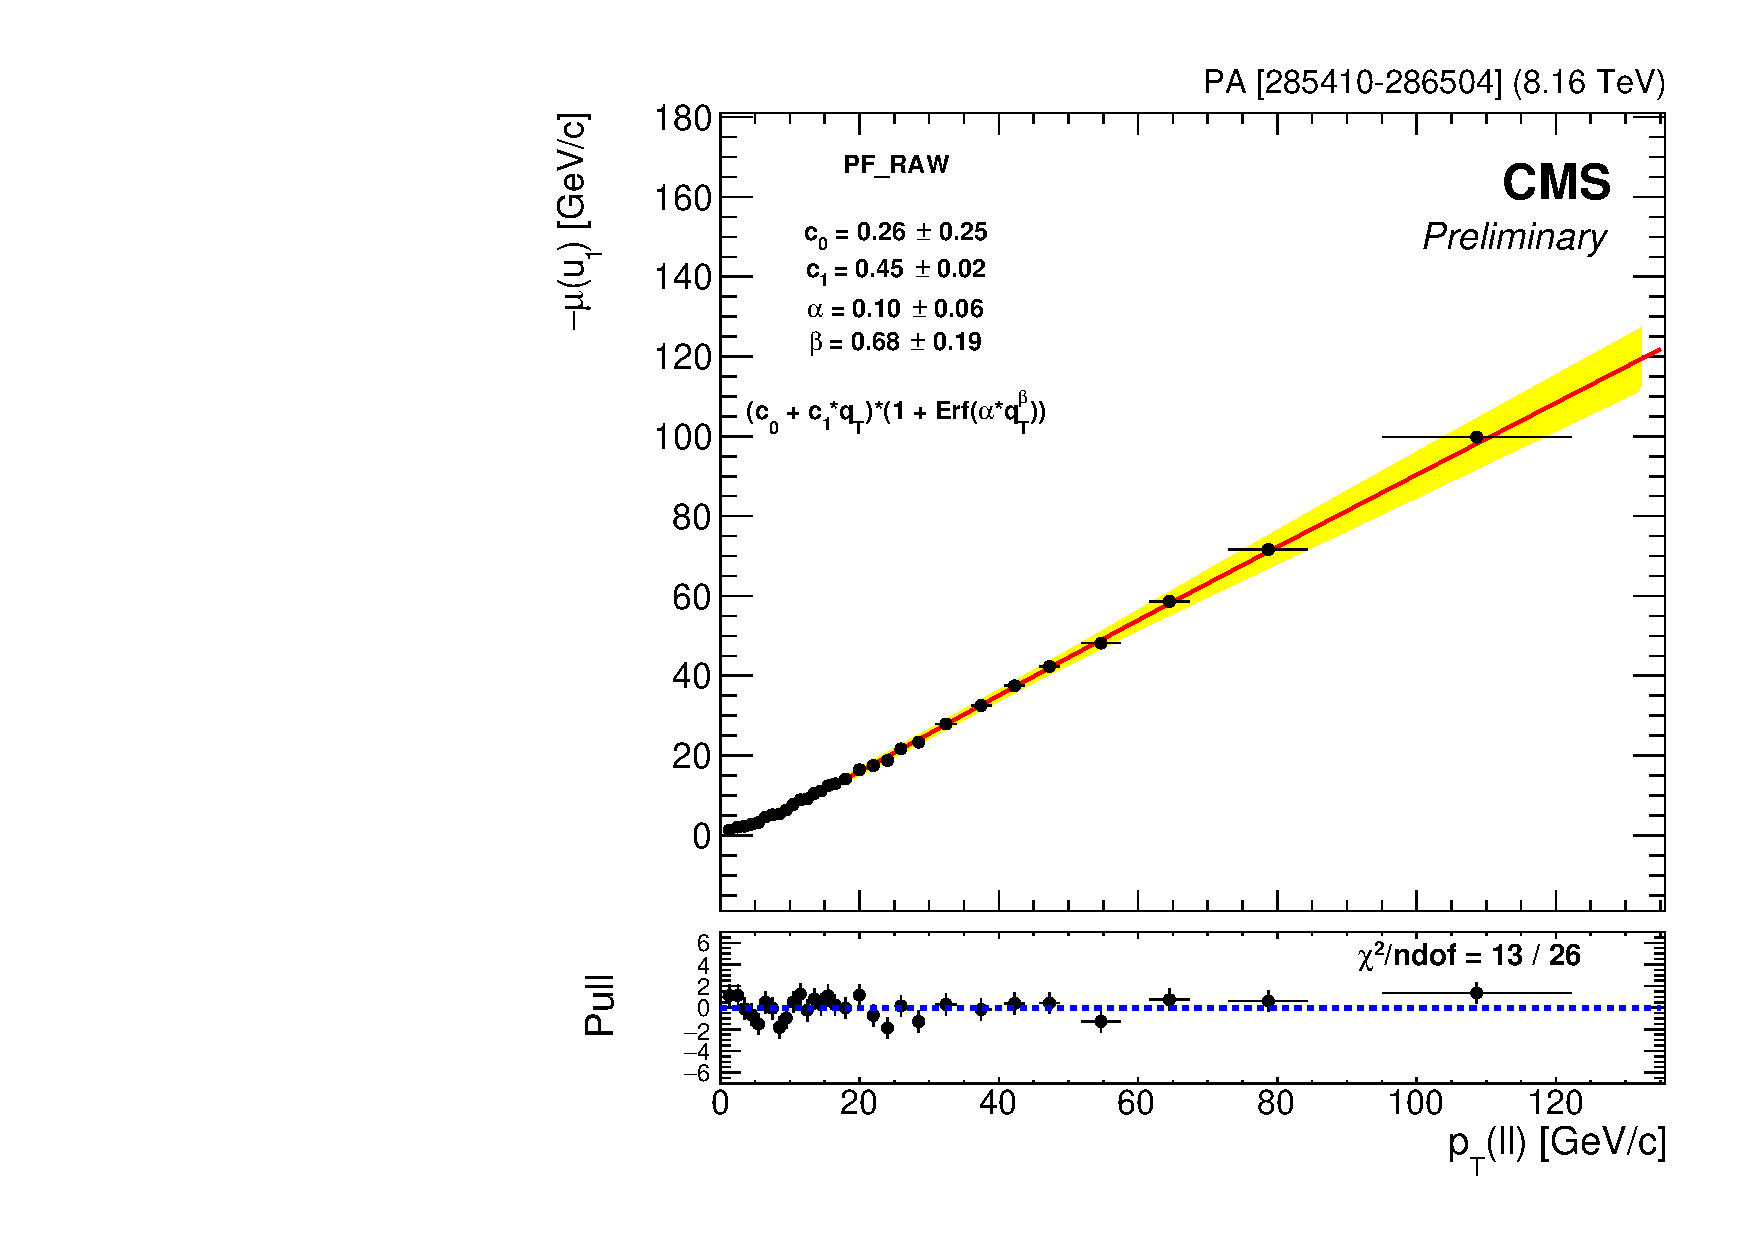
\includegraphics[width=0.3\textwidth]{Figures/WBoson/Analysis/Correction/Recoil/RecoilFitsqT/Data/fitPFu1mean.pdf} \\
  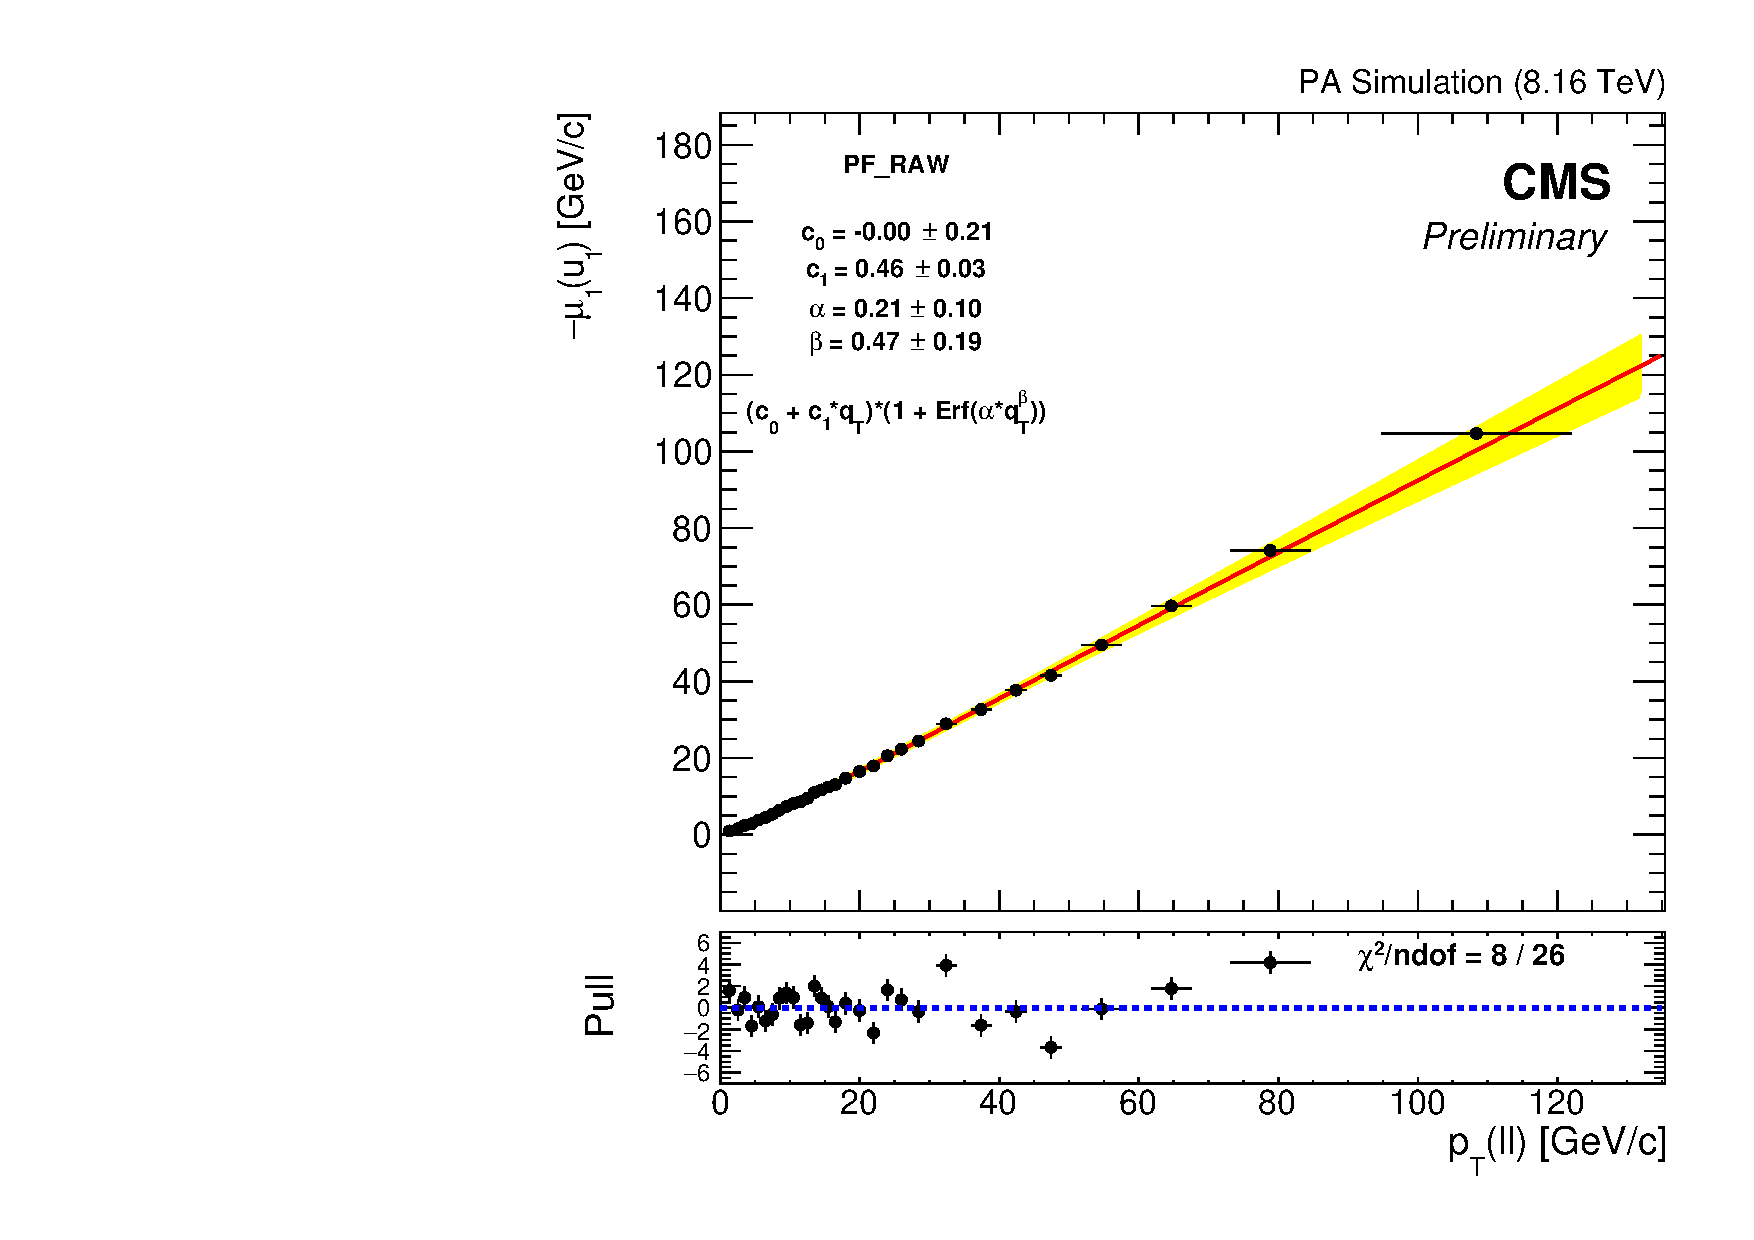
\includegraphics[width=0.3\textwidth]{Figures/WBoson/Analysis/Correction/Recoil/RecoilFitsqT/MC/fitPFu1mean1.pdf}
  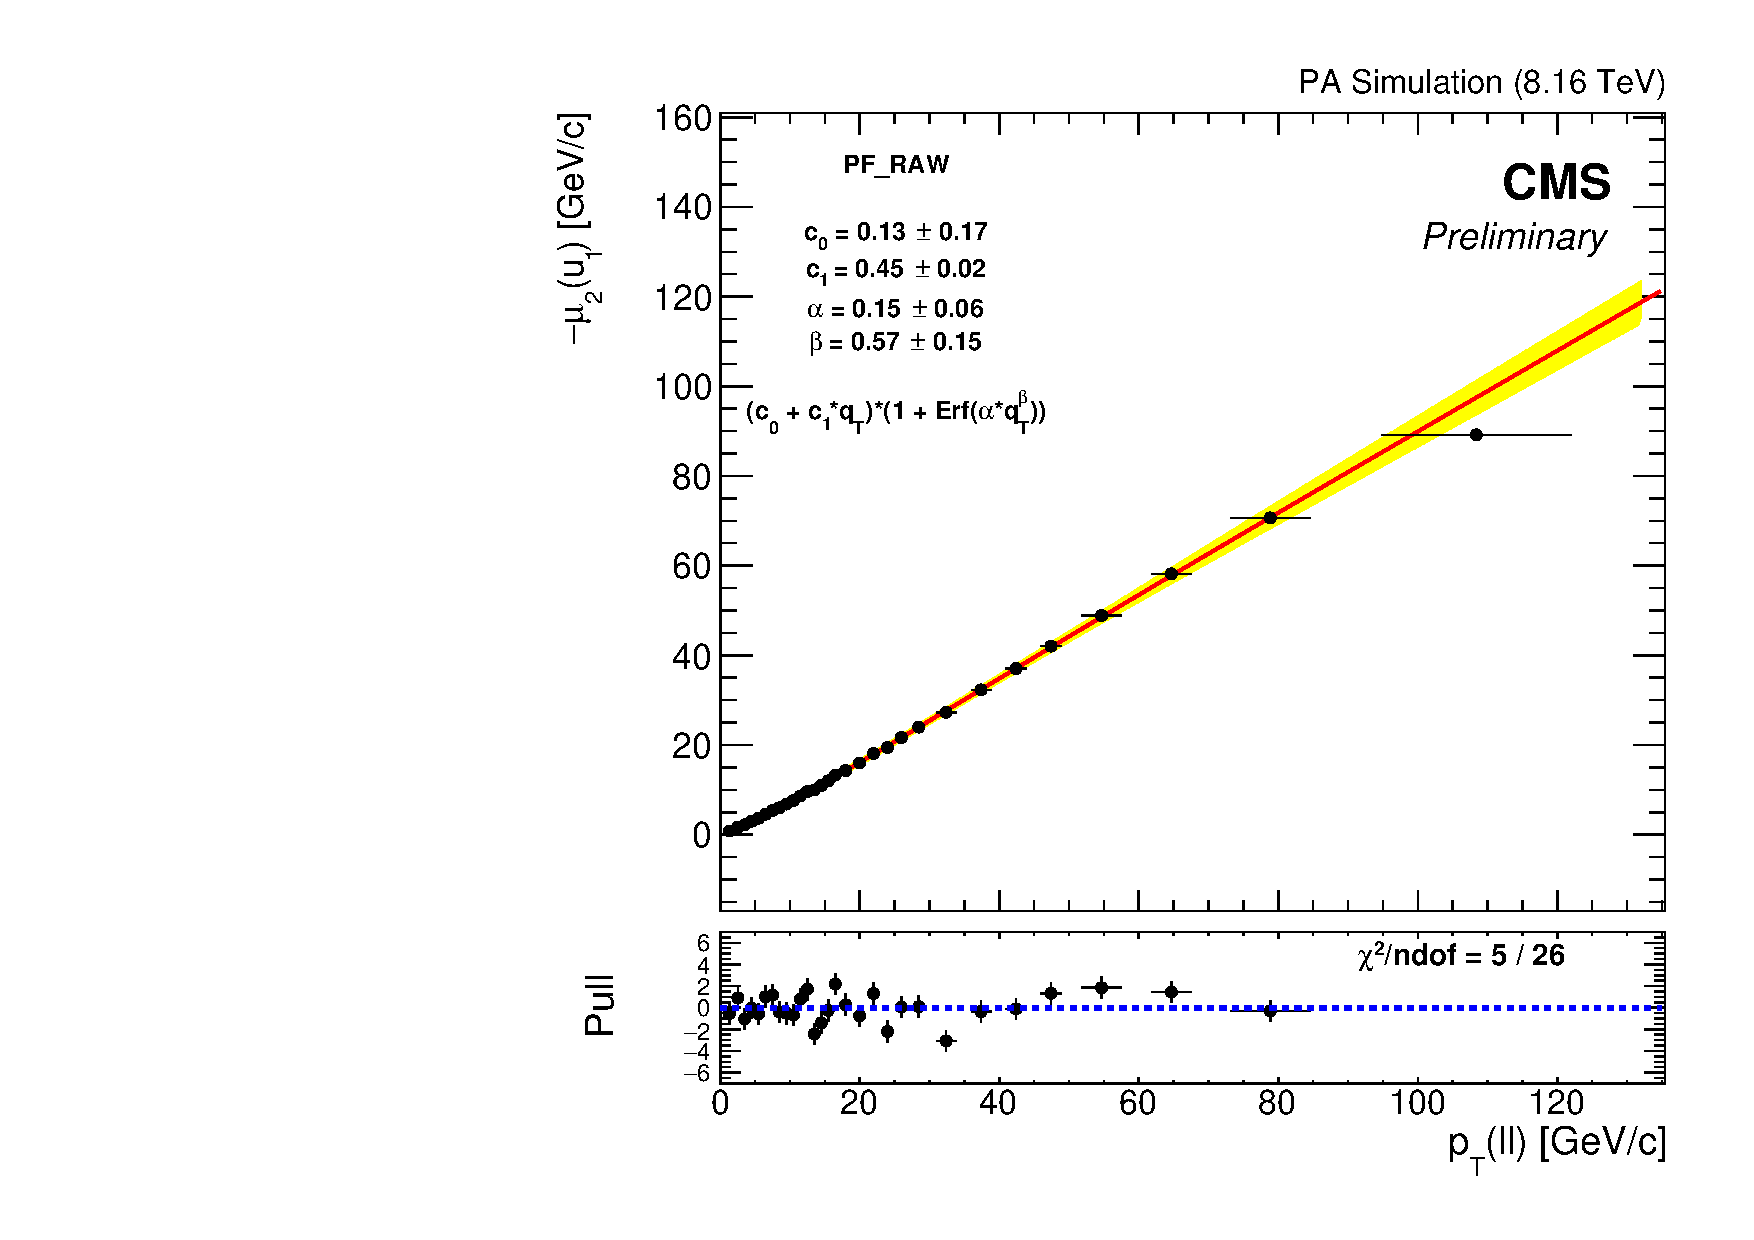
\includegraphics[width=0.3\textwidth]{Figures/WBoson/Analysis/Correction/Recoil/RecoilFitsqT/MC/fitPFu1mean2.pdf}
  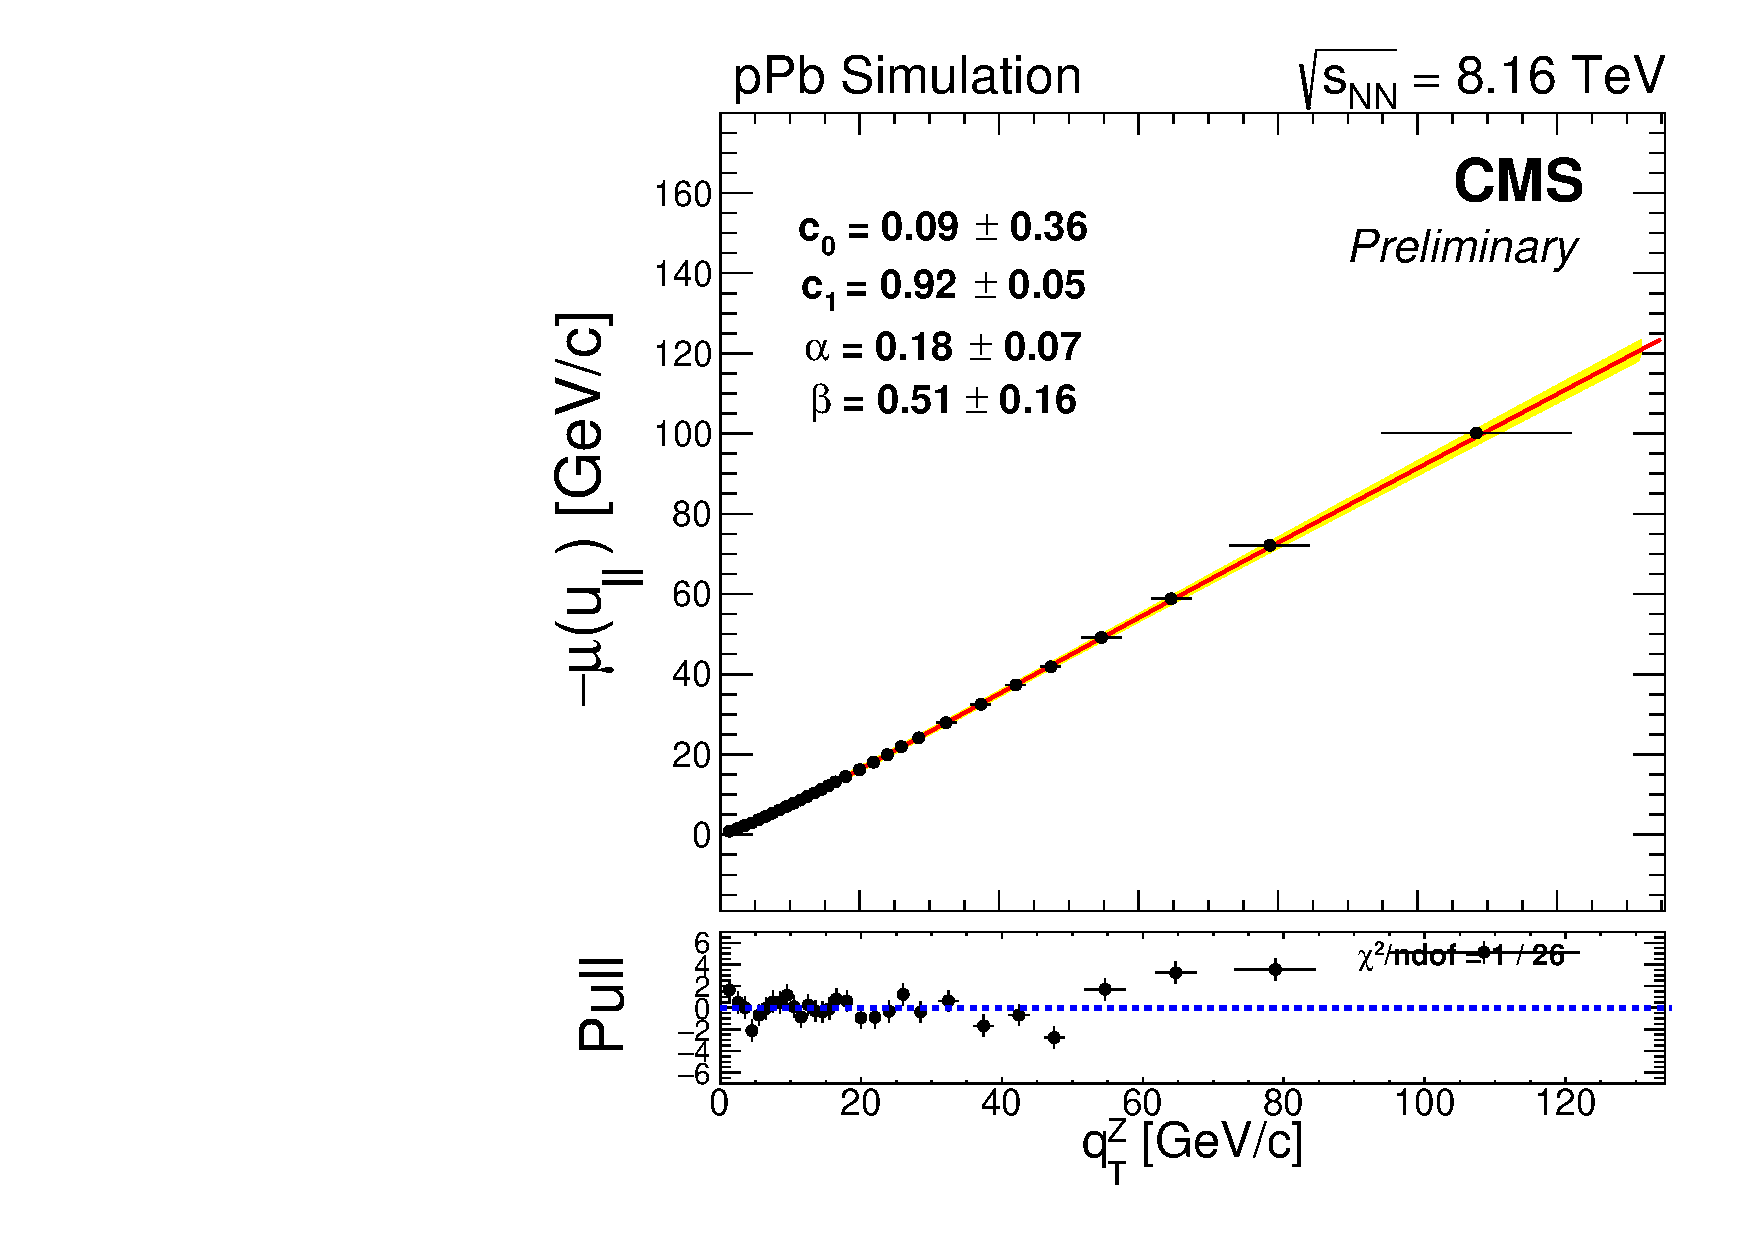
\includegraphics[width=0.3\textwidth]{Figures/WBoson/Analysis/Correction/Recoil/RecoilFitsqT/MC/fitPFu1mean.pdf}
 \caption{Fits for the $\mu_{1}$ (left), $\mu_{2}$ (middle) and weighted average $\mu$ (right) values of the parallel recoil component versus $q_{T}$. The plots on the top correspond to data while the plots in the bottom correspond to \ZToMuMu MC.}
 \label{fig:figU1RecoilScaleFit}
 \end{center}
\end{figure}

The average values of the perpendicular component of the recoil ($u_{2}$) from data and MC \Z samples are fitted with a constant function ($c_{0}$). The outcome is shown in \fig{fig:figU2RecoilScaleFit}. One observe that the average perpendicular component is consistent with zero, and so, it is set to zero in the correction procedure.

\begin{figure}
 \begin{center}
  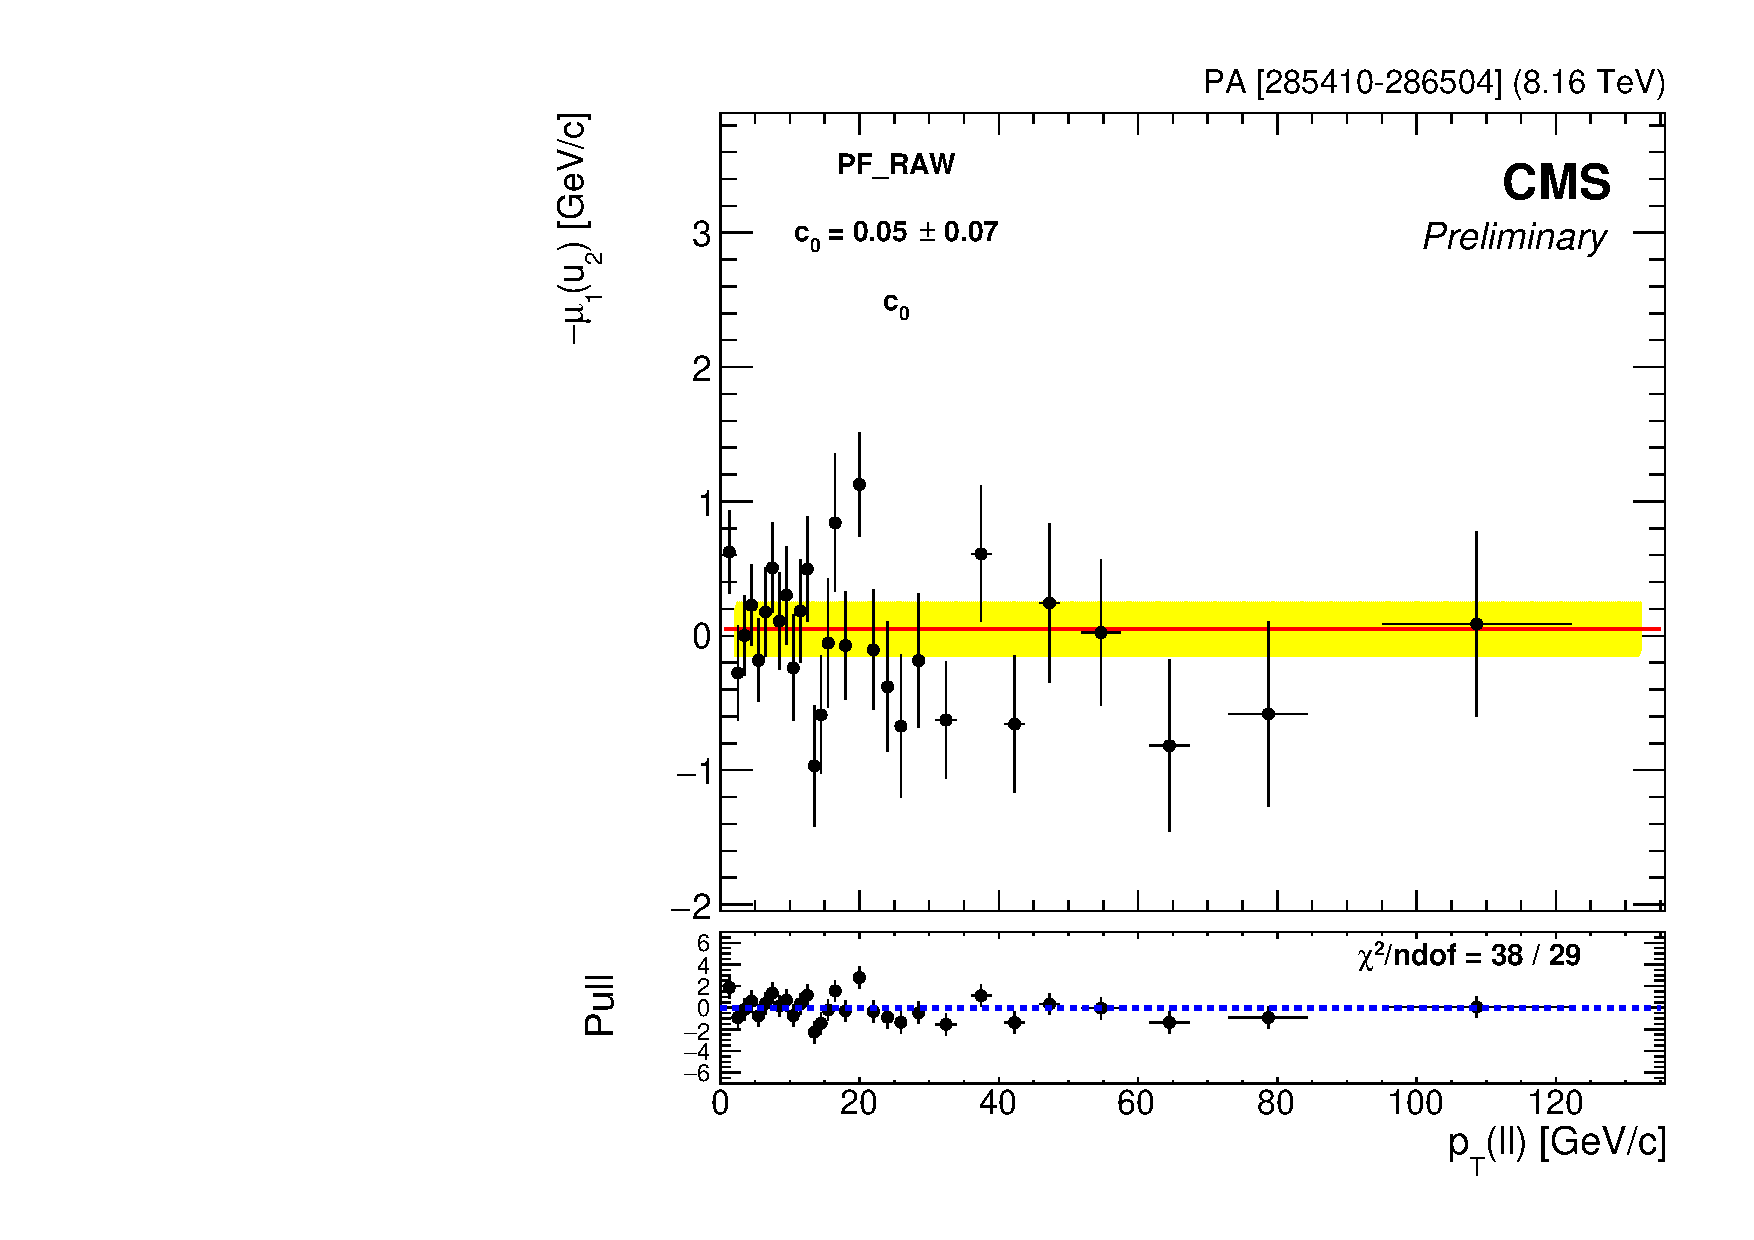
\includegraphics[width=0.3\textwidth]{Figures/WBoson/Analysis/Correction/Recoil/RecoilFitsqT/Data/fitPFu2mean1.pdf}
  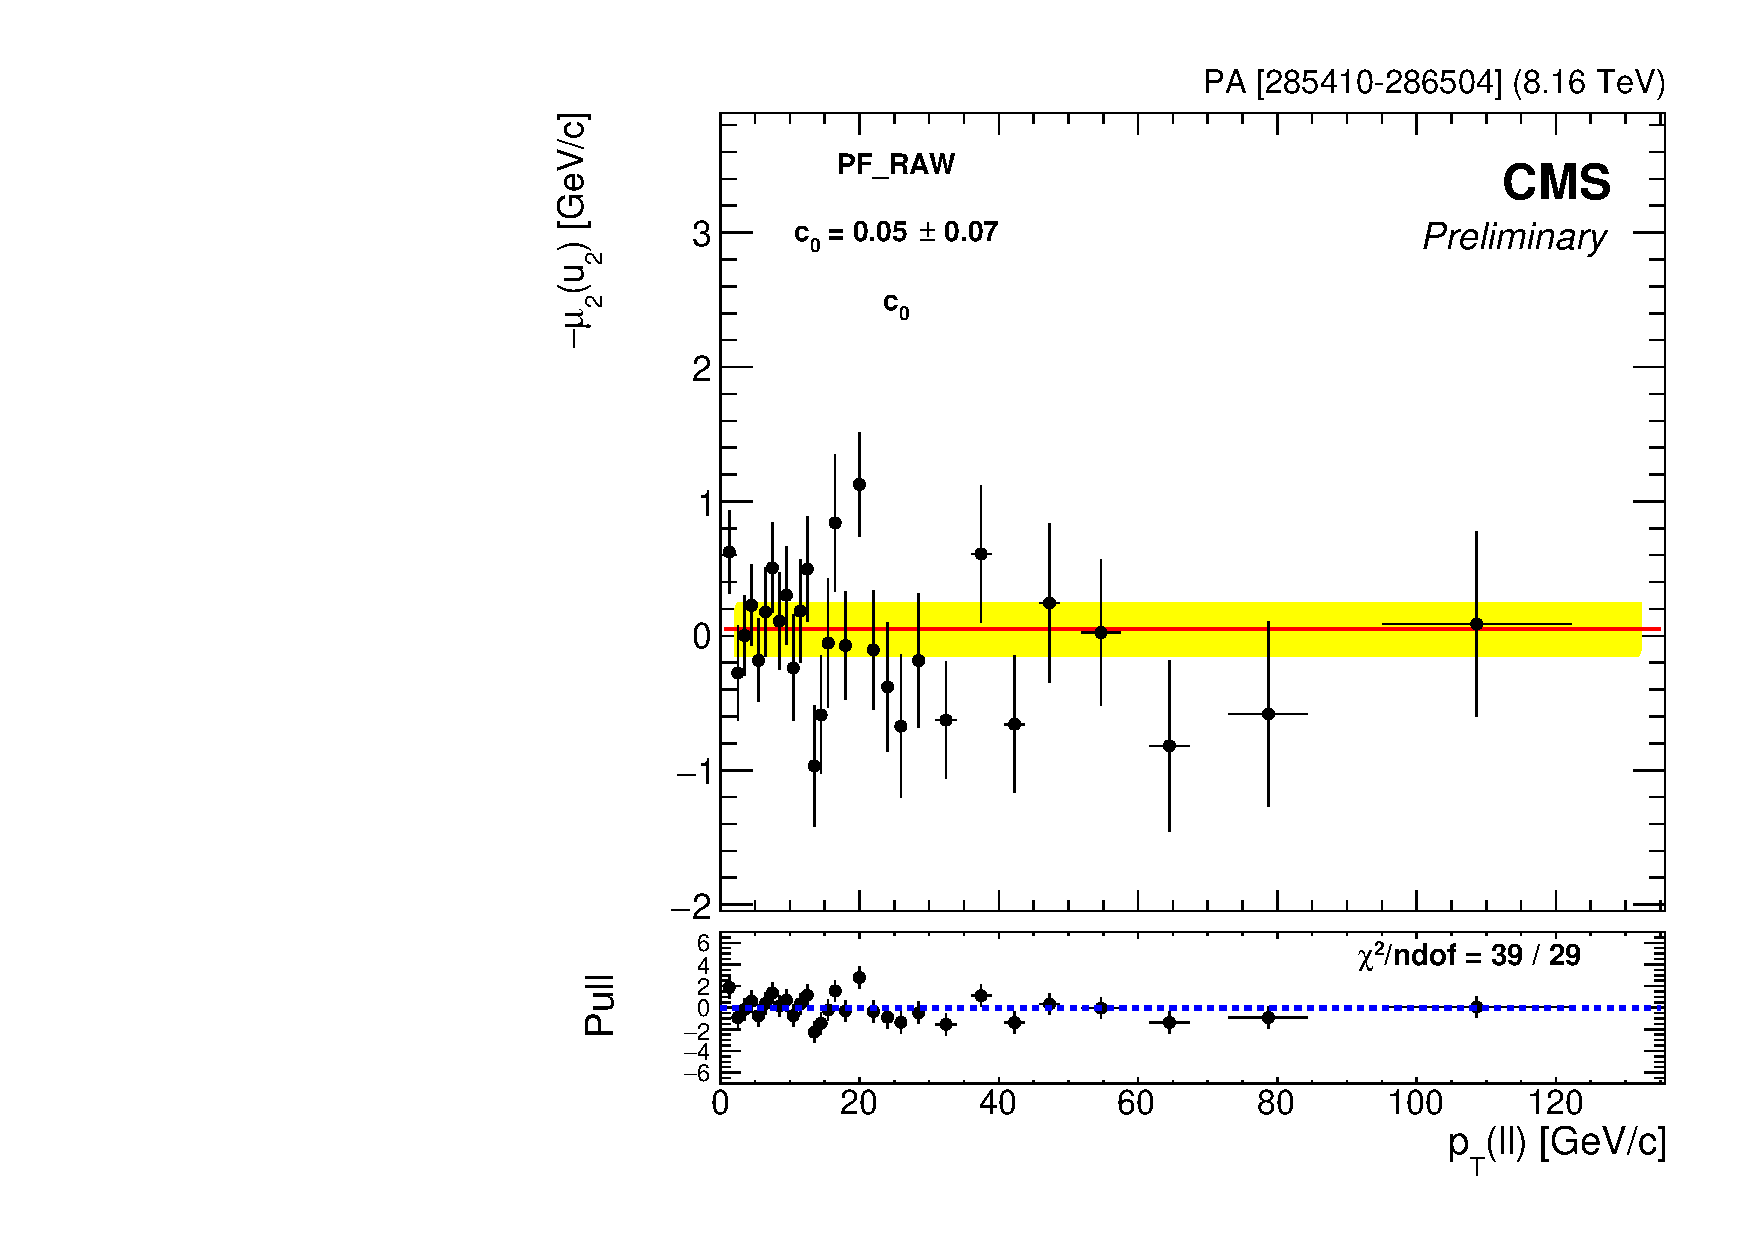
\includegraphics[width=0.3\textwidth]{Figures/WBoson/Analysis/Correction/Recoil/RecoilFitsqT/Data/fitPFu2mean2.pdf}
  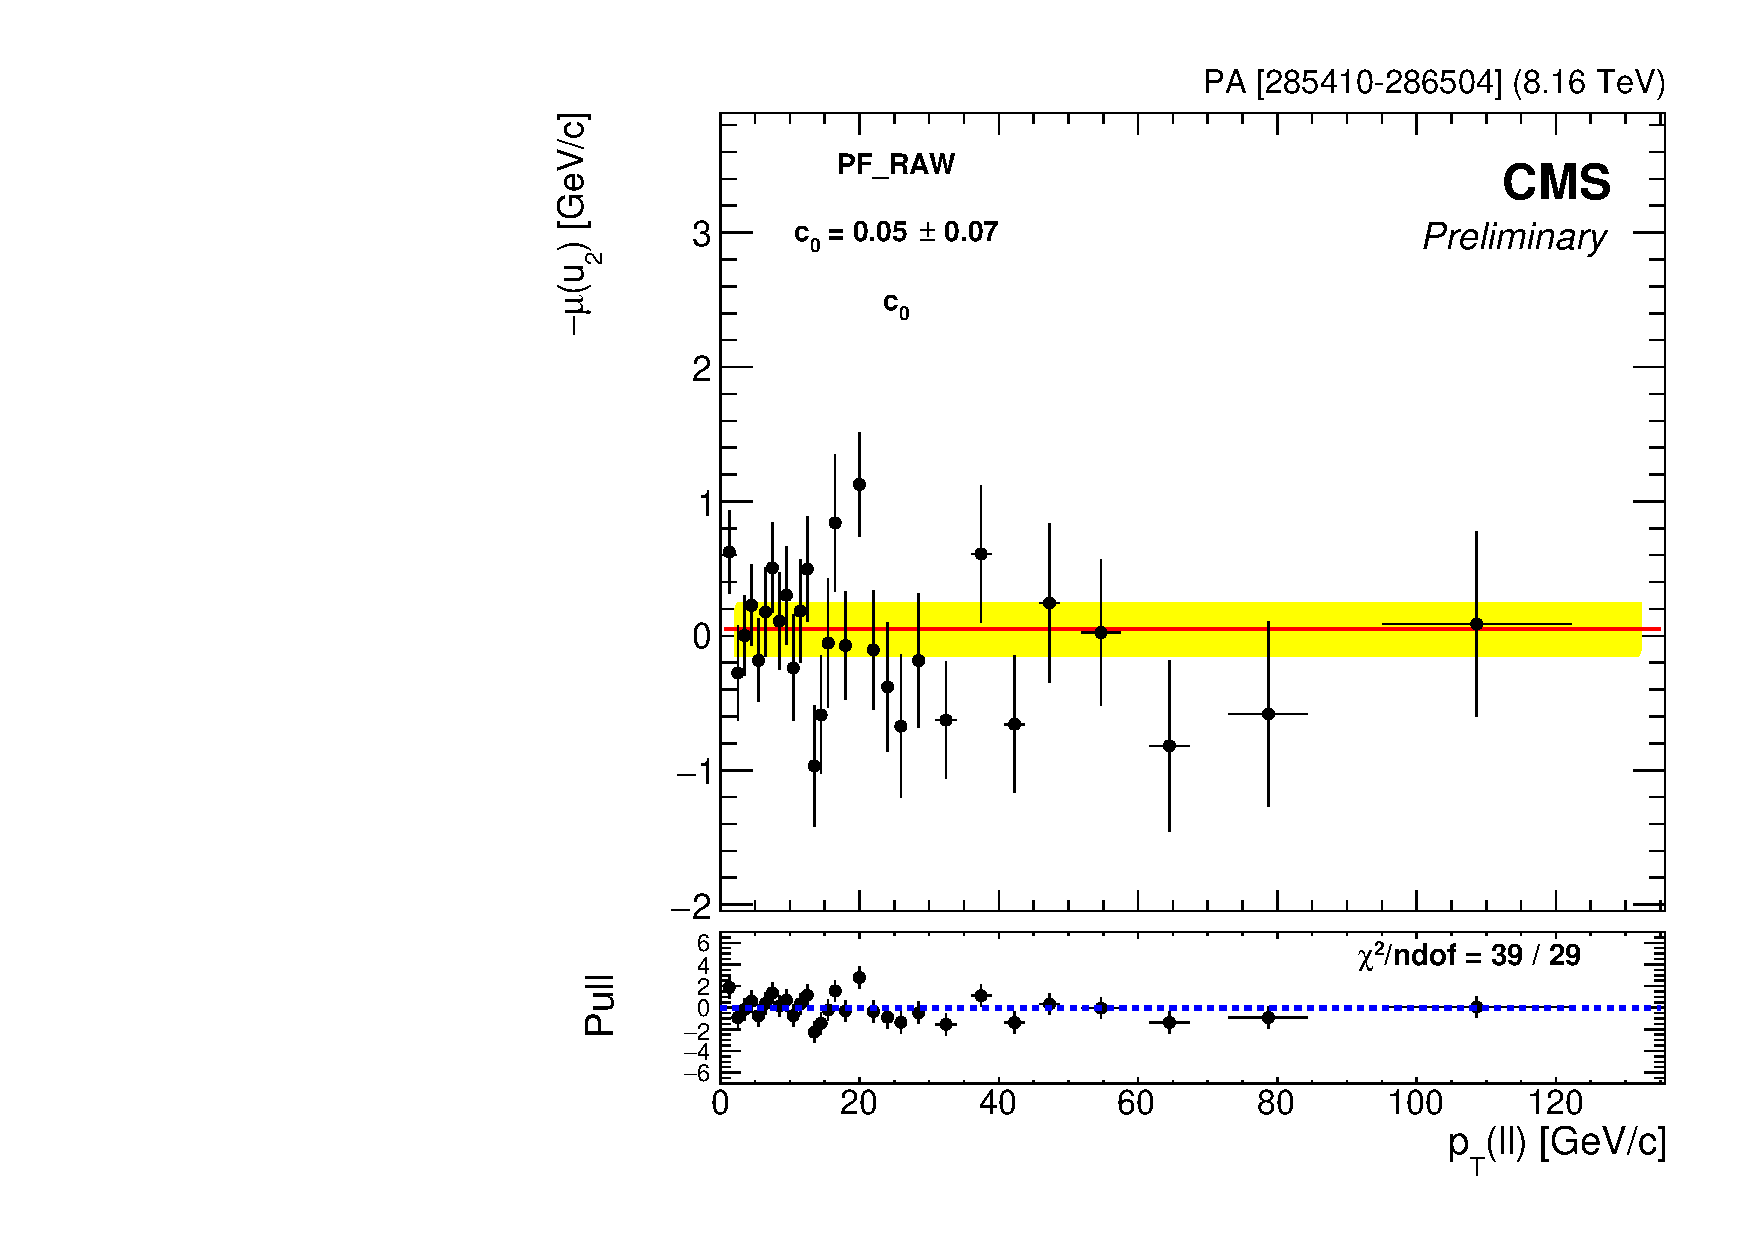
\includegraphics[width=0.3\textwidth]{Figures/WBoson/Analysis/Correction/Recoil/RecoilFitsqT/Data/fitPFu2mean.pdf} \\
  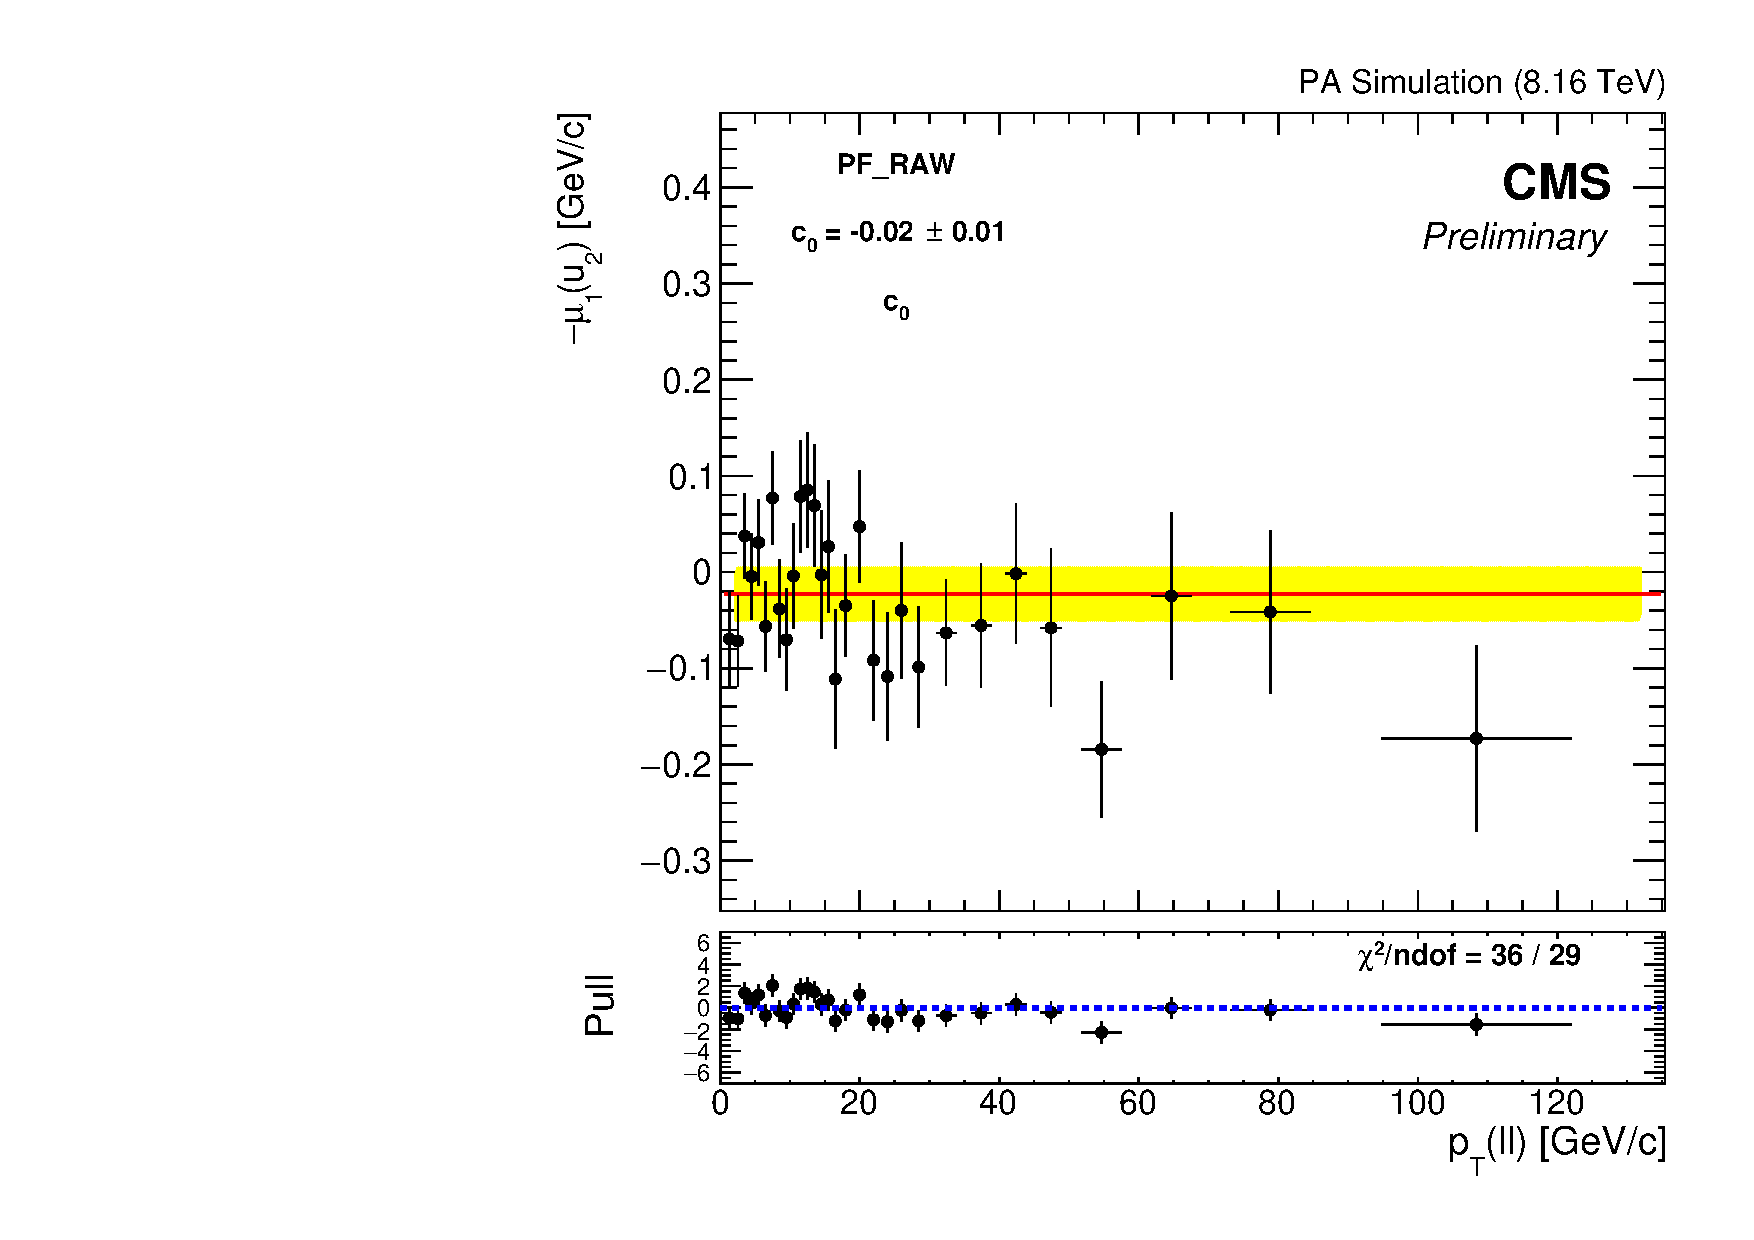
\includegraphics[width=0.3\textwidth]{Figures/WBoson/Analysis/Correction/Recoil/RecoilFitsqT/MC/fitPFu2mean1.pdf}
  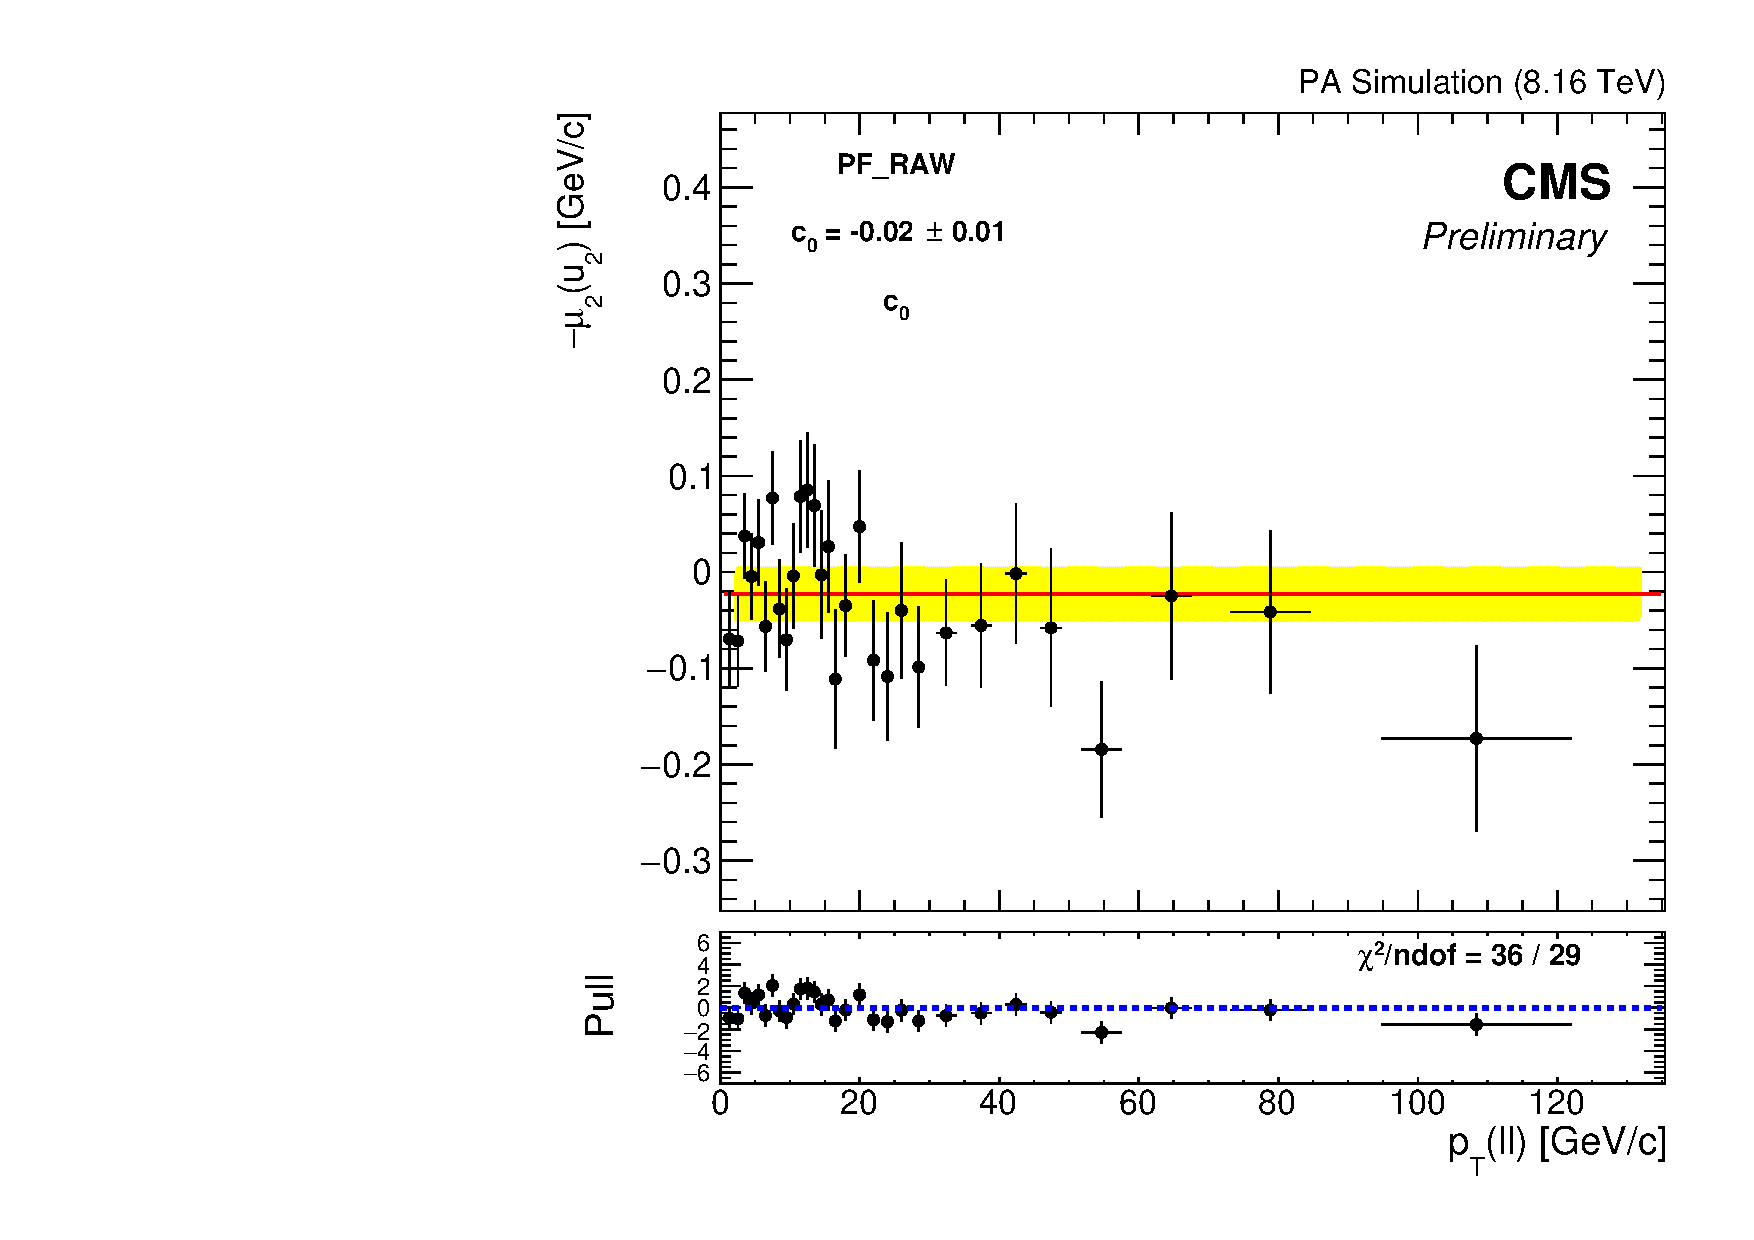
\includegraphics[width=0.3\textwidth]{Figures/WBoson/Analysis/Correction/Recoil/RecoilFitsqT/MC/fitPFu2mean2.pdf}
  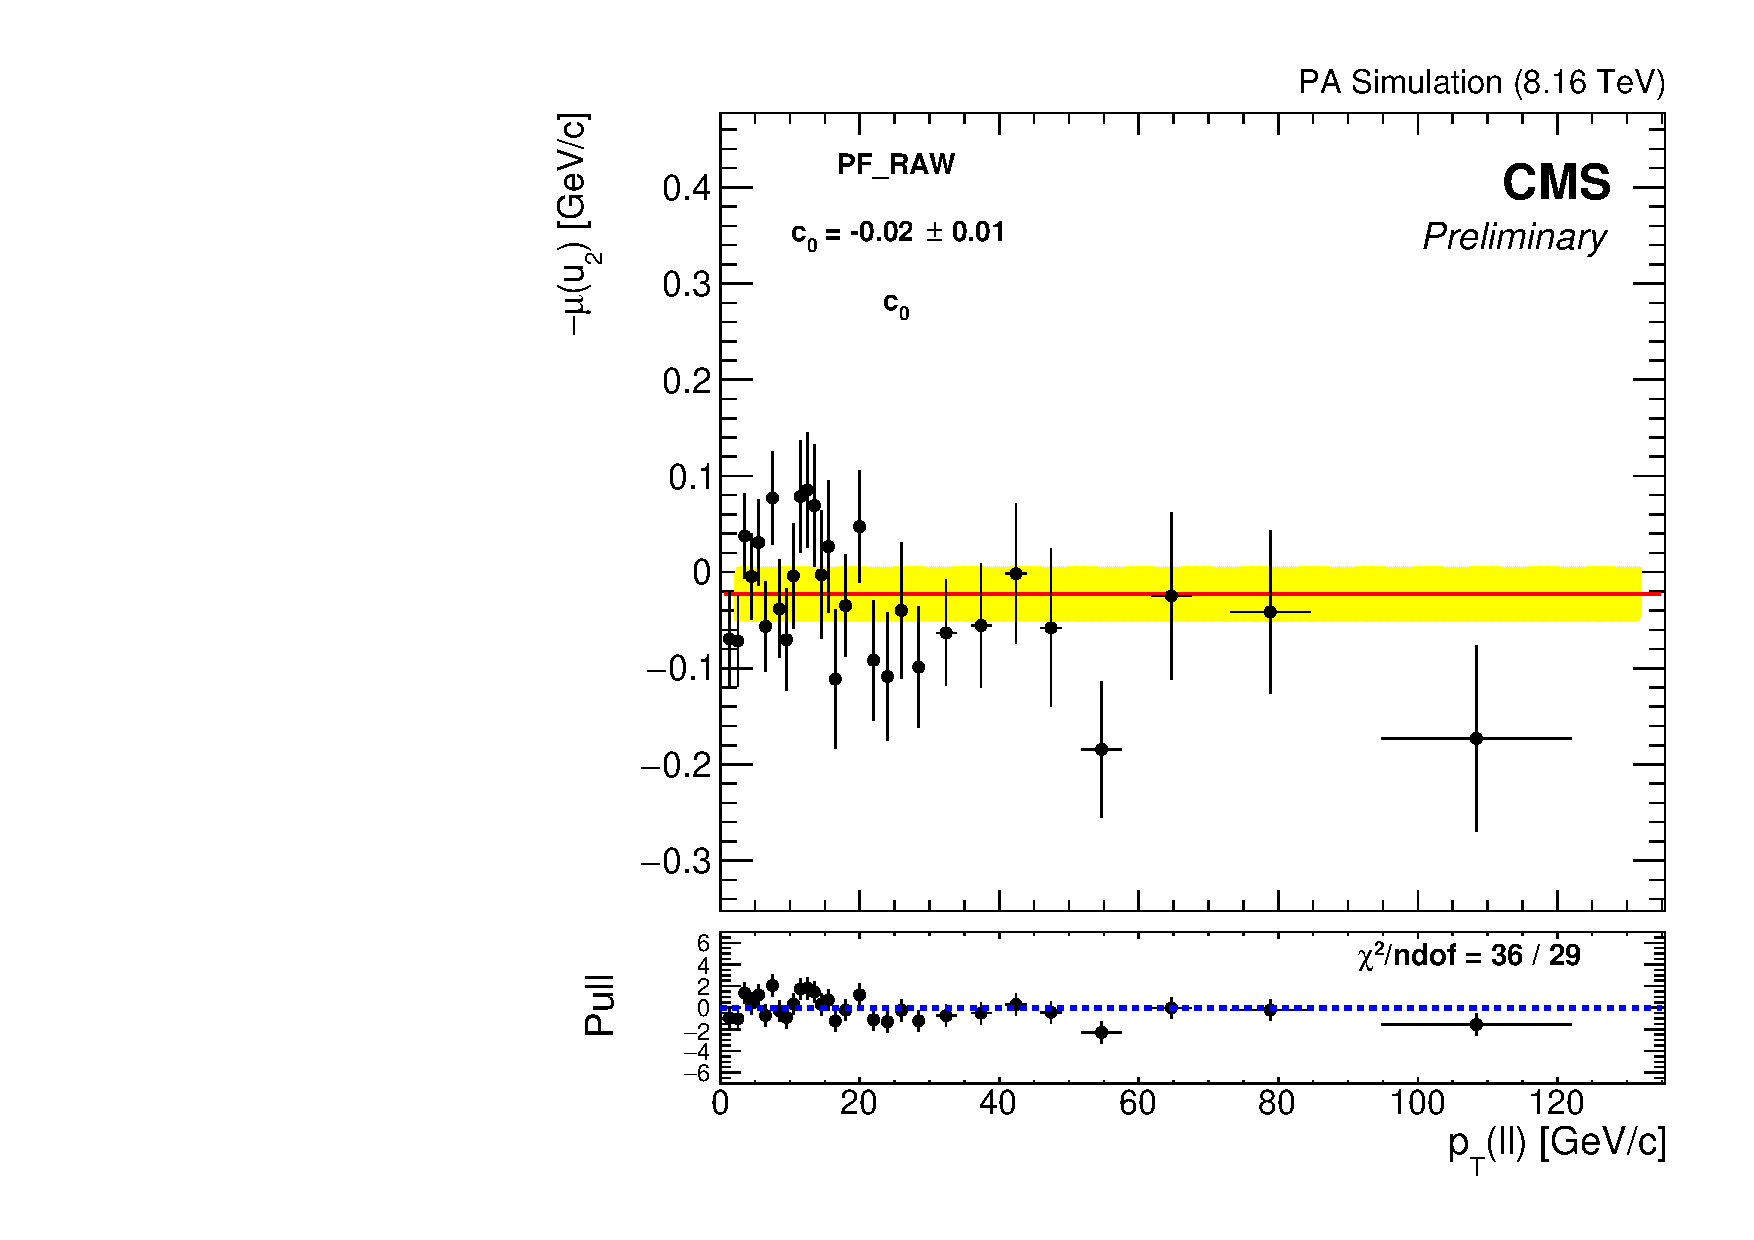
\includegraphics[width=0.3\textwidth]{Figures/WBoson/Analysis/Correction/Recoil/RecoilFitsqT/MC/fitPFu2mean.pdf}
 \caption{Fits for the $\mu_{1}$ (left), $\mu_{2}$ (middle) and weighted average $\mu$ (right) values of the perpendicular recoil component versus $q_{T}$. The plots on the top correspond to data while the plots in the bottom correspond to \ZToMuMu MC.}
 \label{fig:figU2RecoilScaleFit}
 \end{center}
\end{figure}


\subsubsection{Recoil Resolution}\label{sec:WBoson_Corrections_MET_Rres}

The gaussian widths ($\sigma_{1}$ and $\sigma_{2}$) of the parallel and perpendicular distributions of the recoil are also extracted from the recoil fits for each $q_{T}$ bin. The recoil resolution is   parametrised as a function of $q_{T}$ using the following formula:

\begin{equation}\label{eq:equreolnparam} 
\sigma_{1,2}(q_{T}) = \sqrt{s_{0}^{2} + s_{1}^{2} \cdot q_{T}^{\alpha}},
\end{equation}

The fits to the resolution profile of the parallel and perpendicular components of the recoil are presented in \fig{fig:figU1RecoilResolutionFit} and  \fig{fig:figU2RecoilResolutionFit}, respectively. Moreover, the distribution of the weighted average of the two gaussian widths, $\sigma = f \cdot \sigma_{1} + (1 - f) \cdot \sigma_{2}$, is also shown.

\begin{figure} [h!]
 \begin{center}
  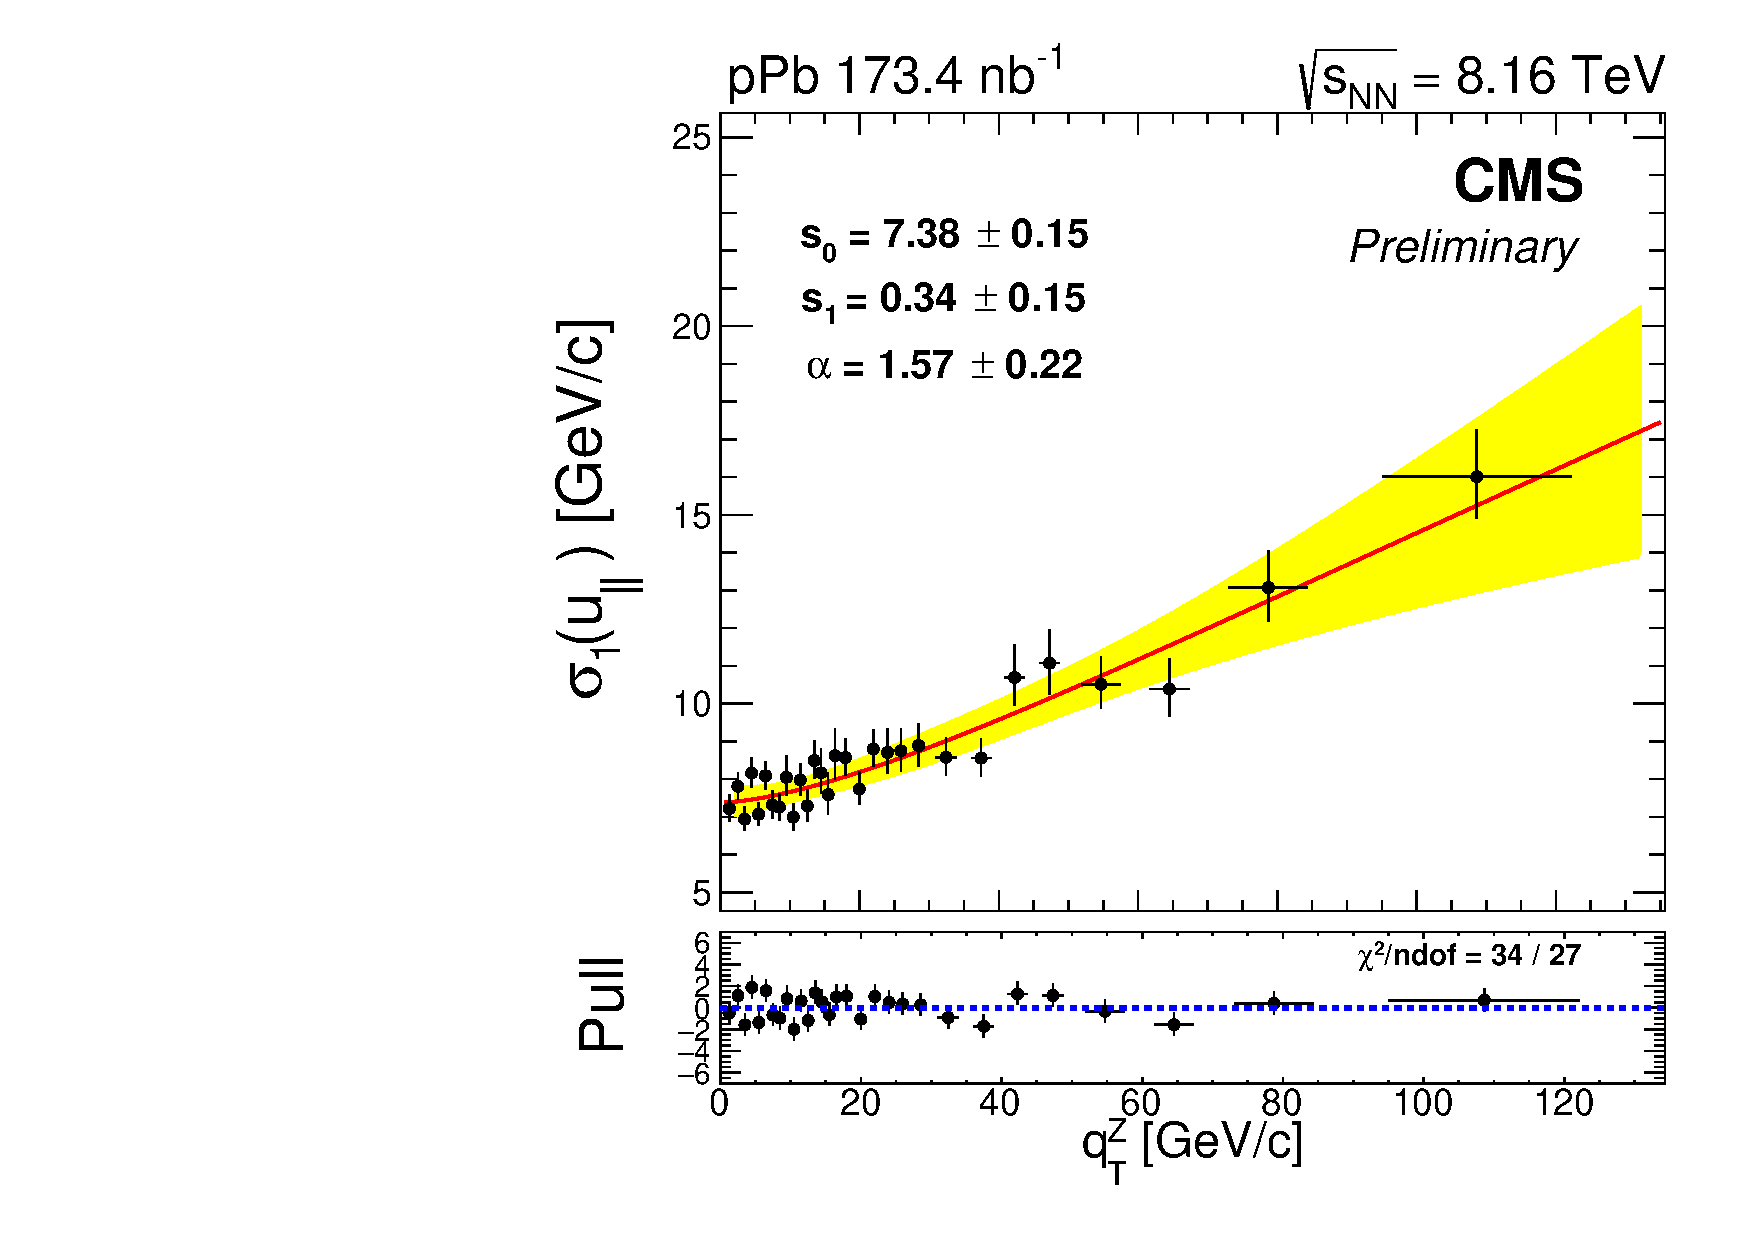
\includegraphics[width=0.3\textwidth]{Figures/WBoson/Analysis/Correction/Recoil/RecoilFitsqT/Data/fitPFu1sigma1.pdf}
  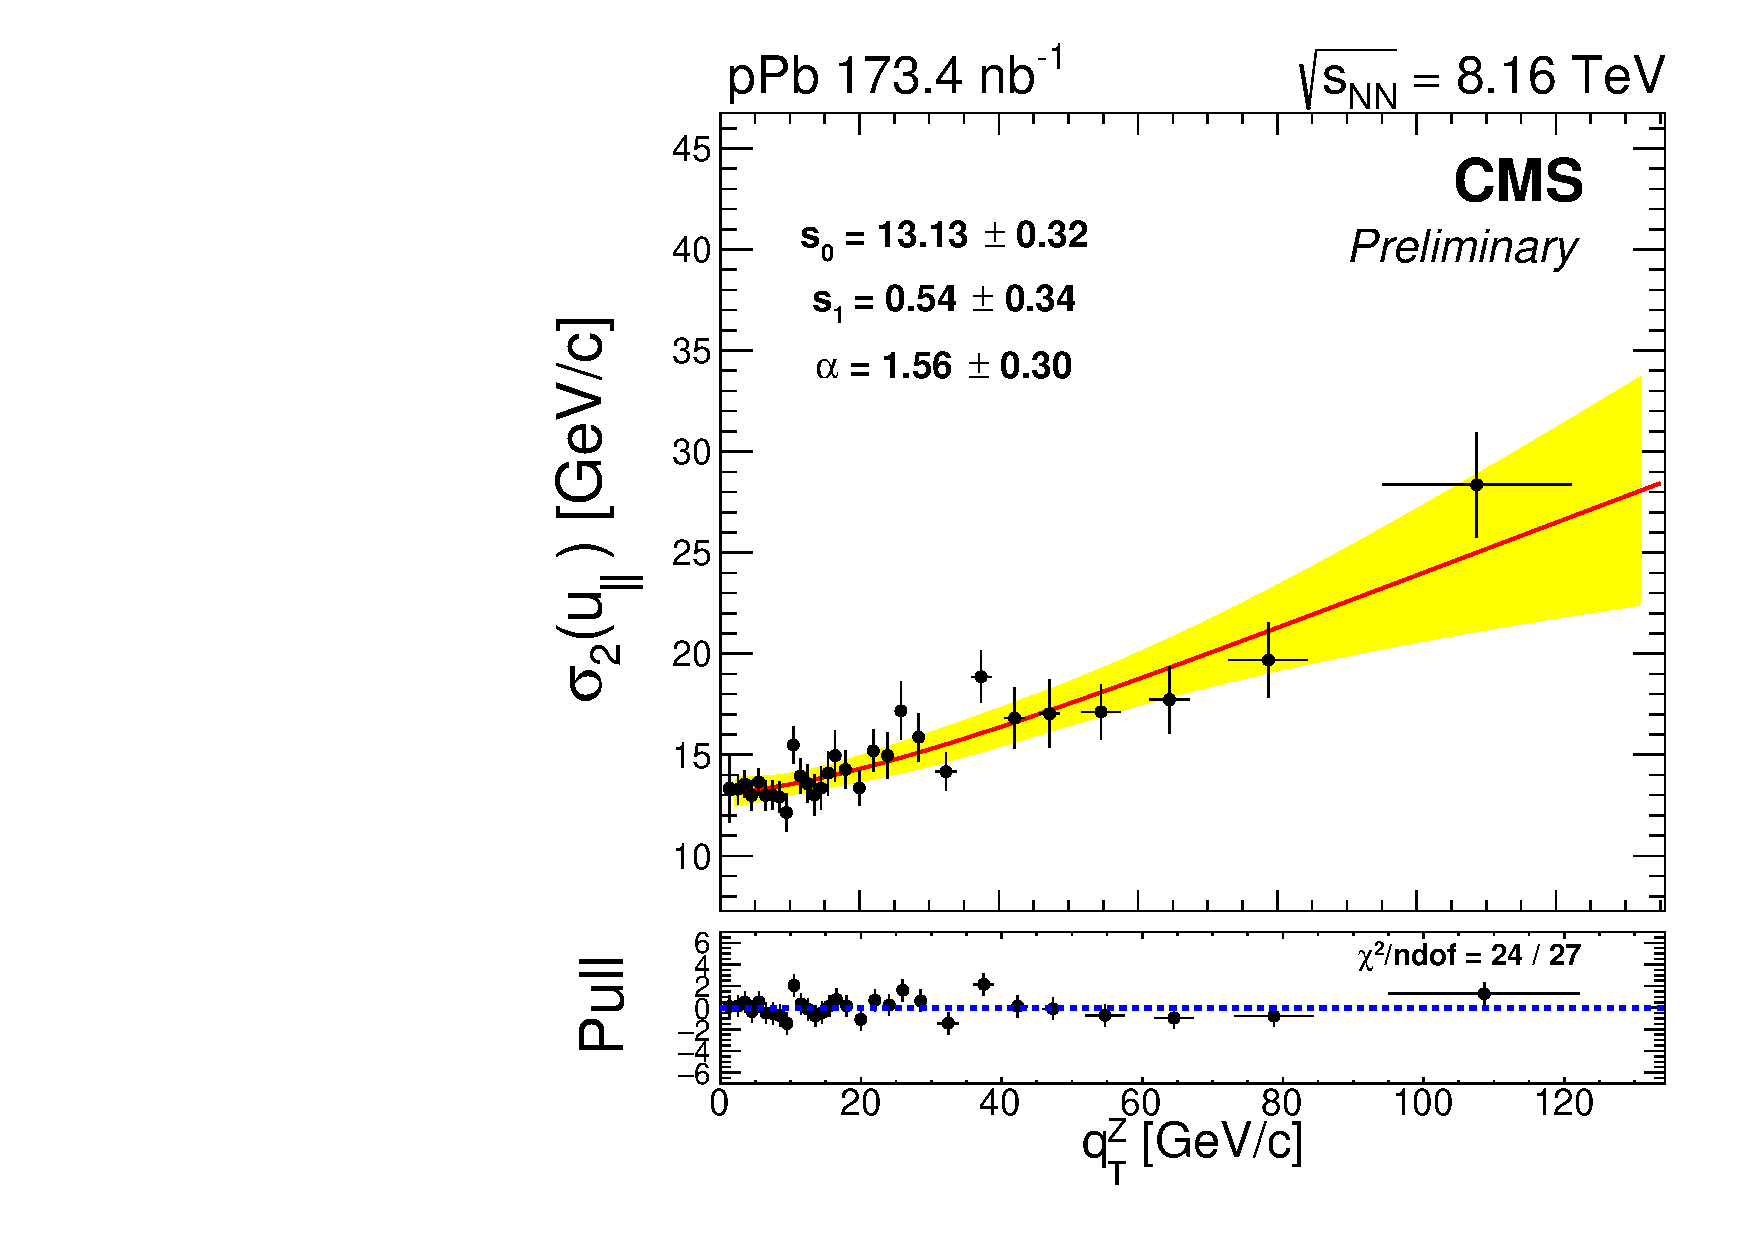
\includegraphics[width=0.3\textwidth]{Figures/WBoson/Analysis/Correction/Recoil/RecoilFitsqT/Data/fitPFu1sigma2.pdf}
  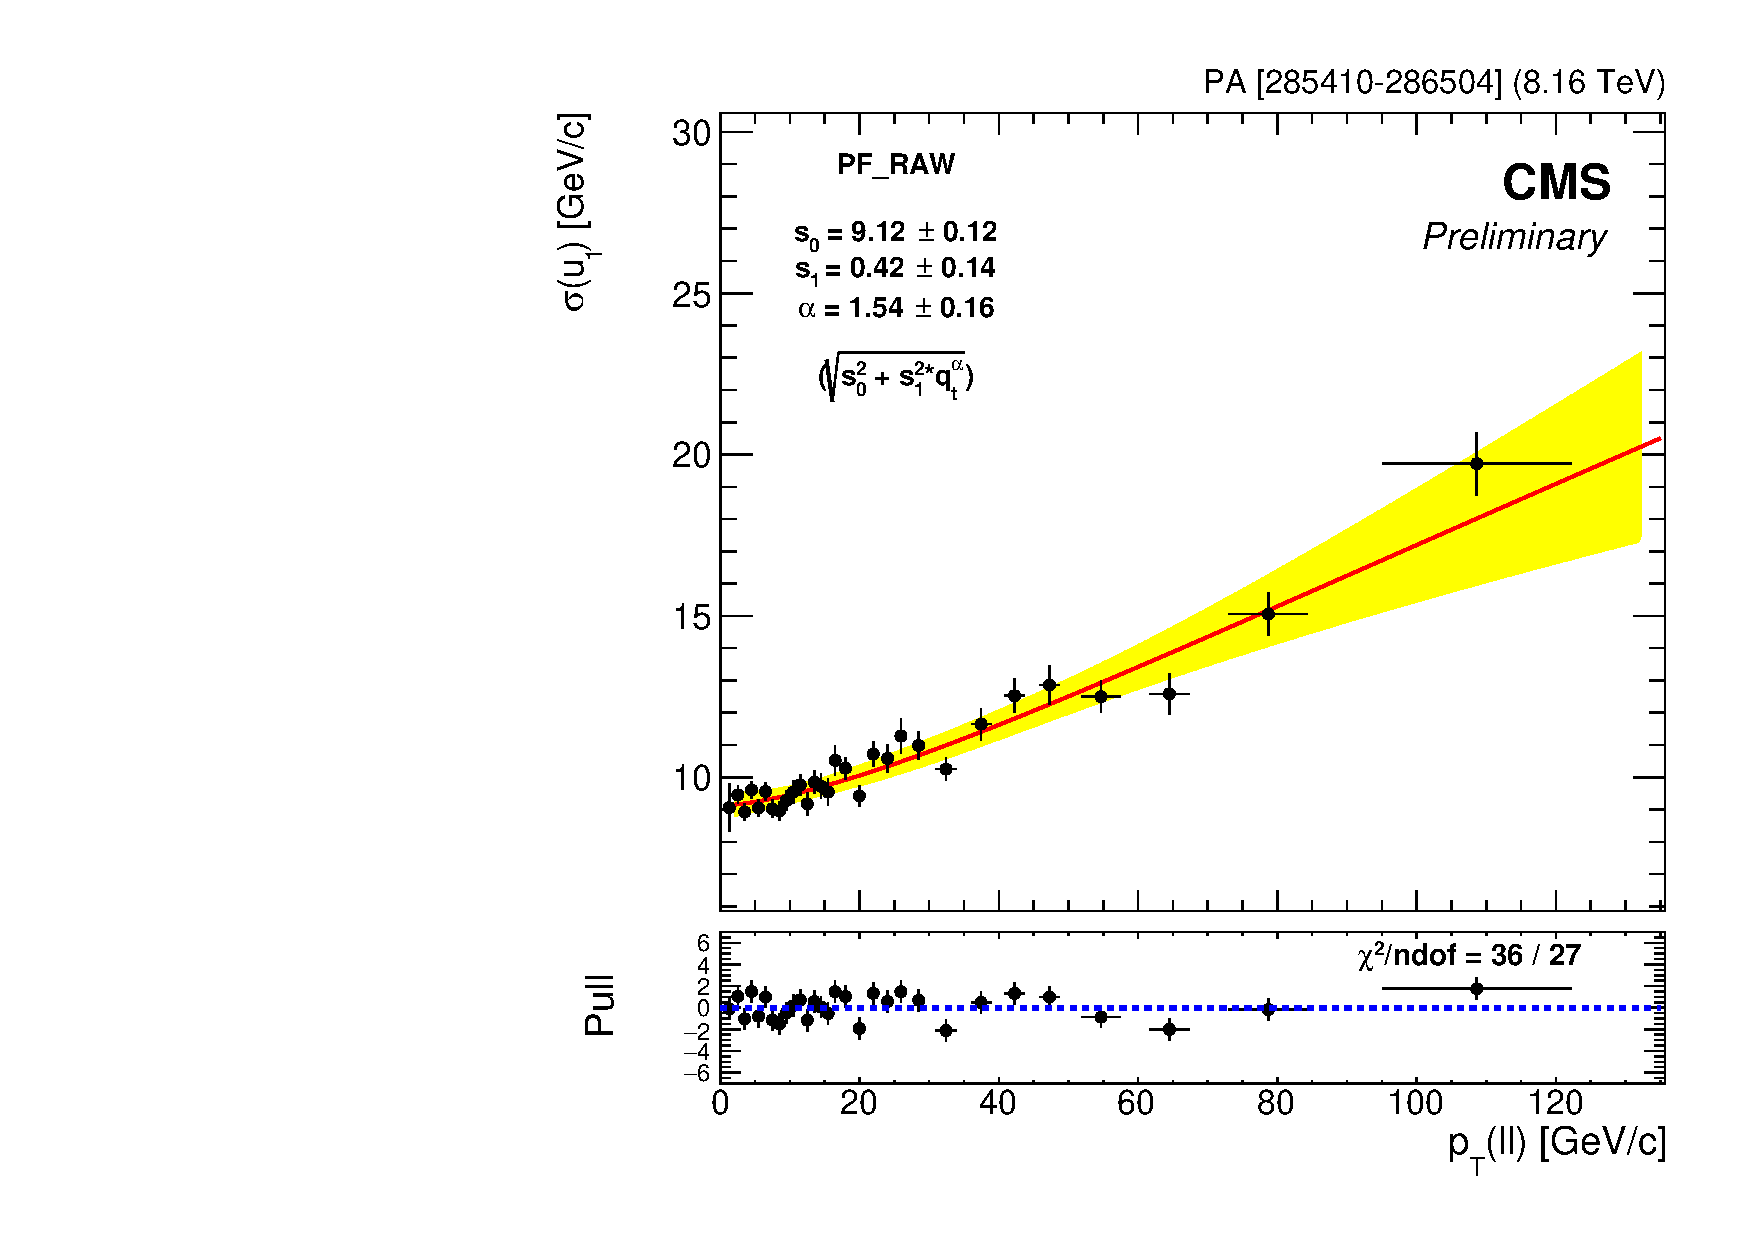
\includegraphics[width=0.3\textwidth]{Figures/WBoson/Analysis/Correction/Recoil/RecoilFitsqT/Data/fitPFu1sigma.pdf} \\
  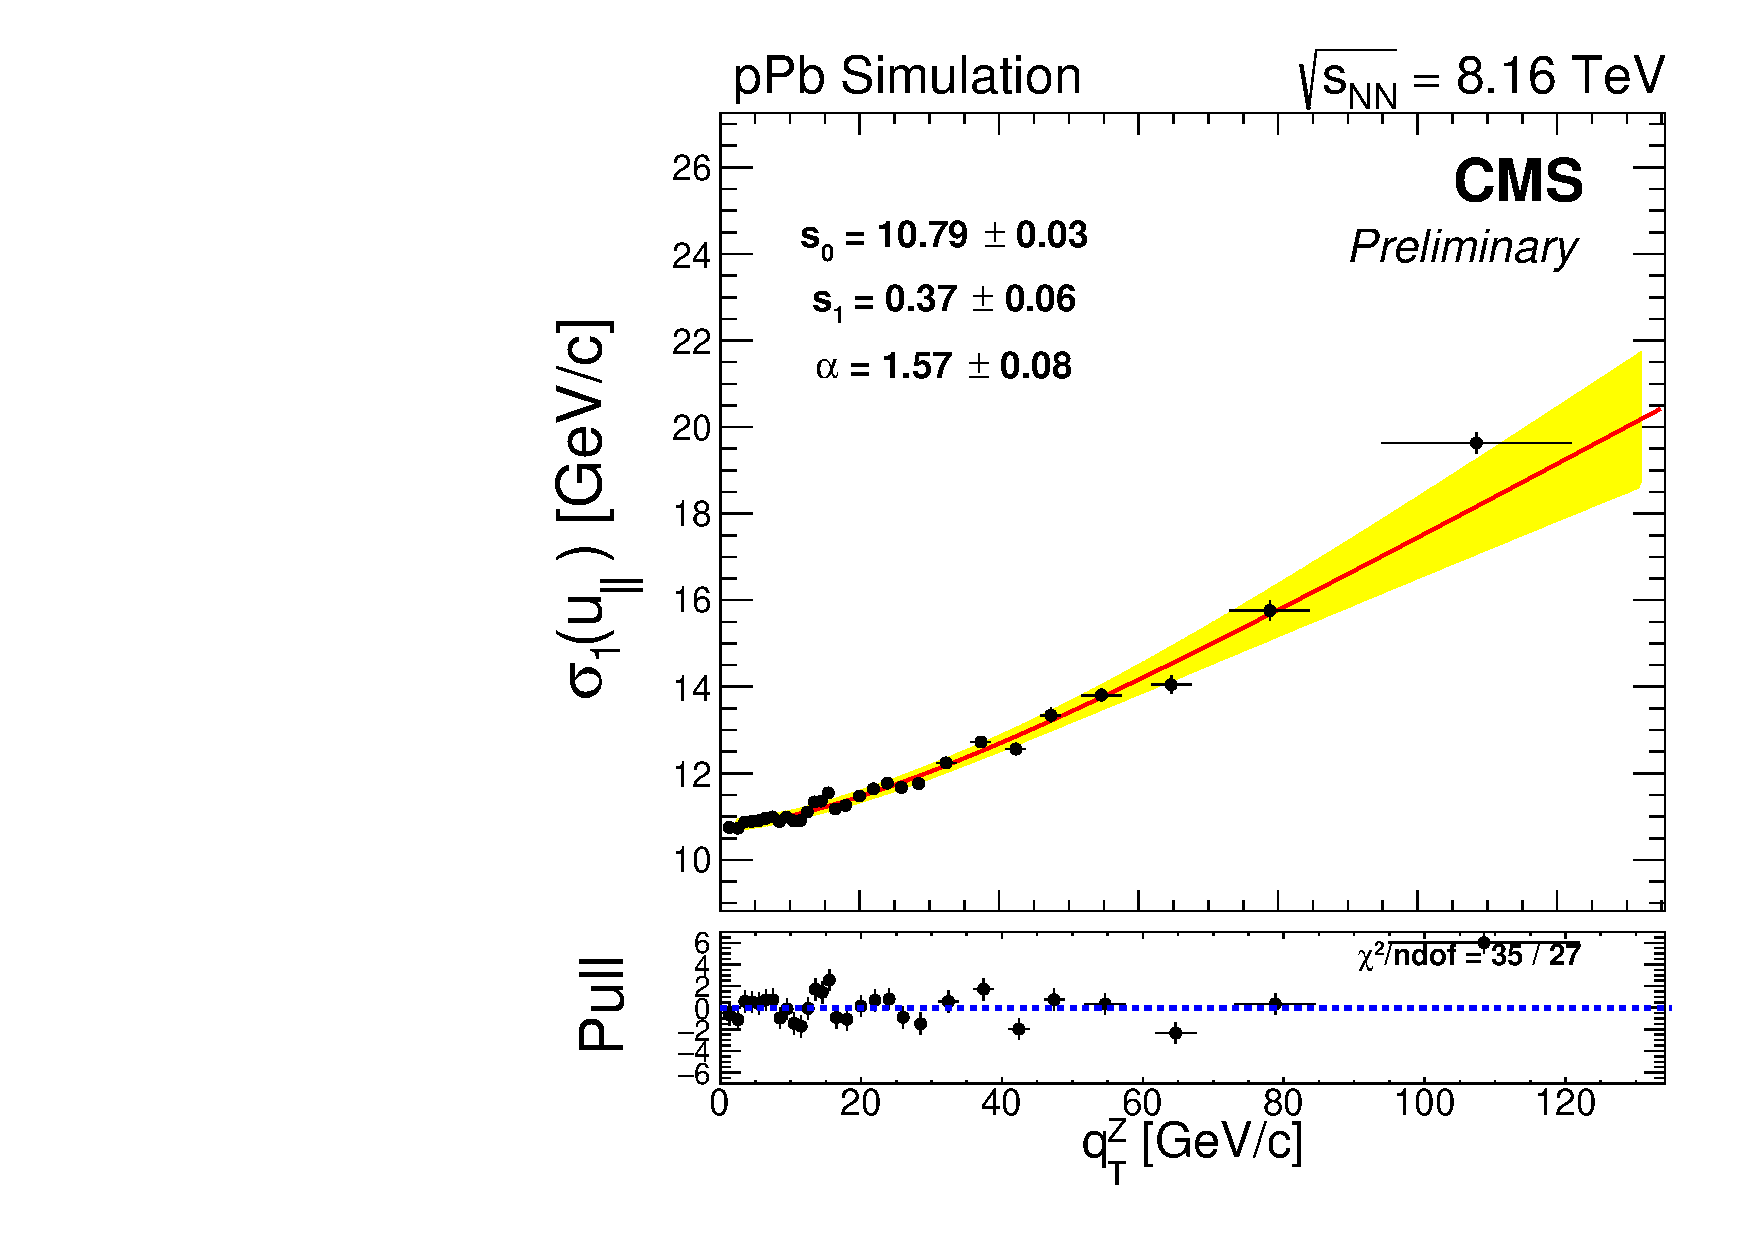
\includegraphics[width=0.3\textwidth]{Figures/WBoson/Analysis/Correction/Recoil/RecoilFitsqT/MC/fitPFu1sigma1.pdf}
  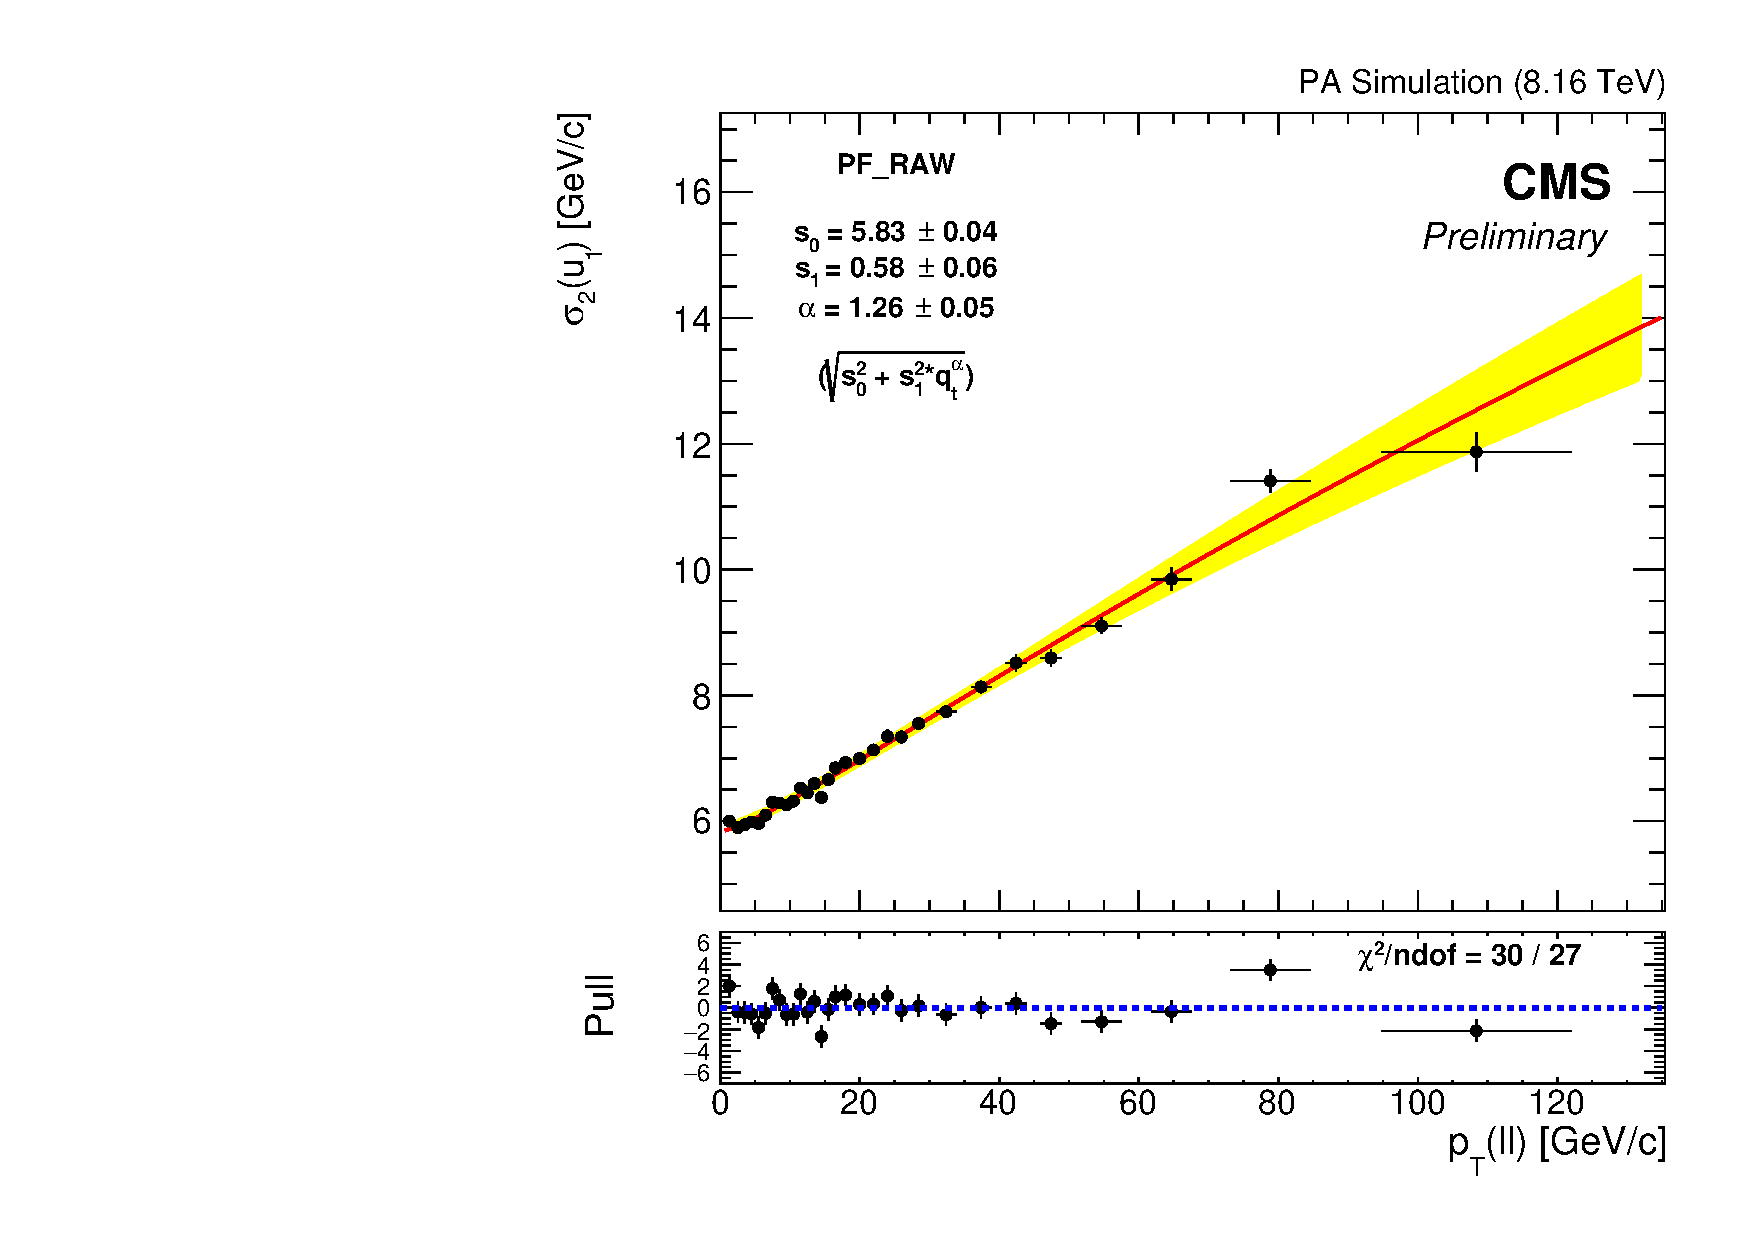
\includegraphics[width=0.3\textwidth]{Figures/WBoson/Analysis/Correction/Recoil/RecoilFitsqT/MC/fitPFu1sigma2.pdf}
  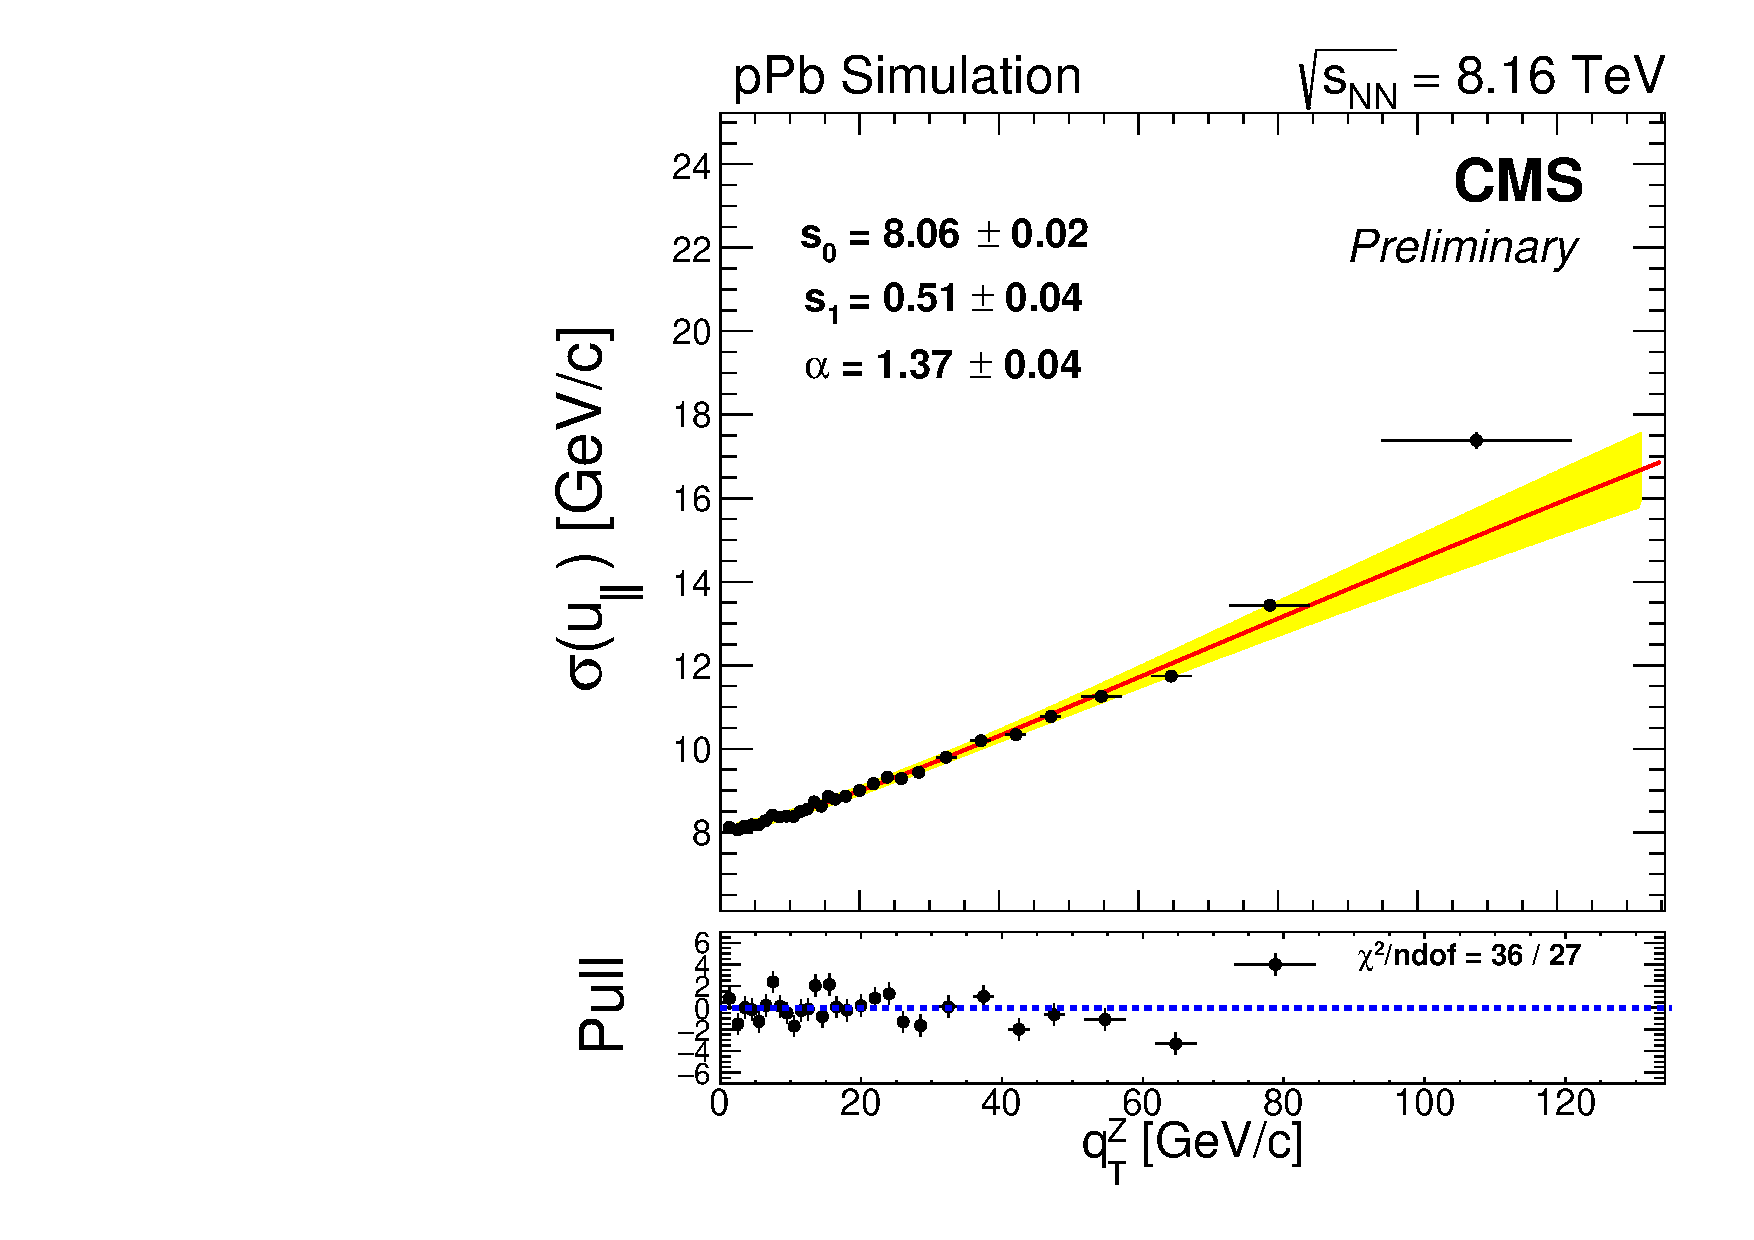
\includegraphics[width=0.3\textwidth]{Figures/WBoson/Analysis/Correction/Recoil/RecoilFitsqT/MC/fitPFu1sigma.pdf}
 \caption{Fits for the $\sigma_{1}$ (left), $\sigma_{2}$ (middle) and weighted average $\sigma$ (right) values of the parallel recoil component versus $q_{T}$. The plots on the top correspond to data while the plots in the bottom correspond to \ZToMuMu MC.}
 \label{fig:figU1RecoilResolutionFit}
 \end{center}
\end{figure}

\begin{figure} [h!]
 \begin{center}
  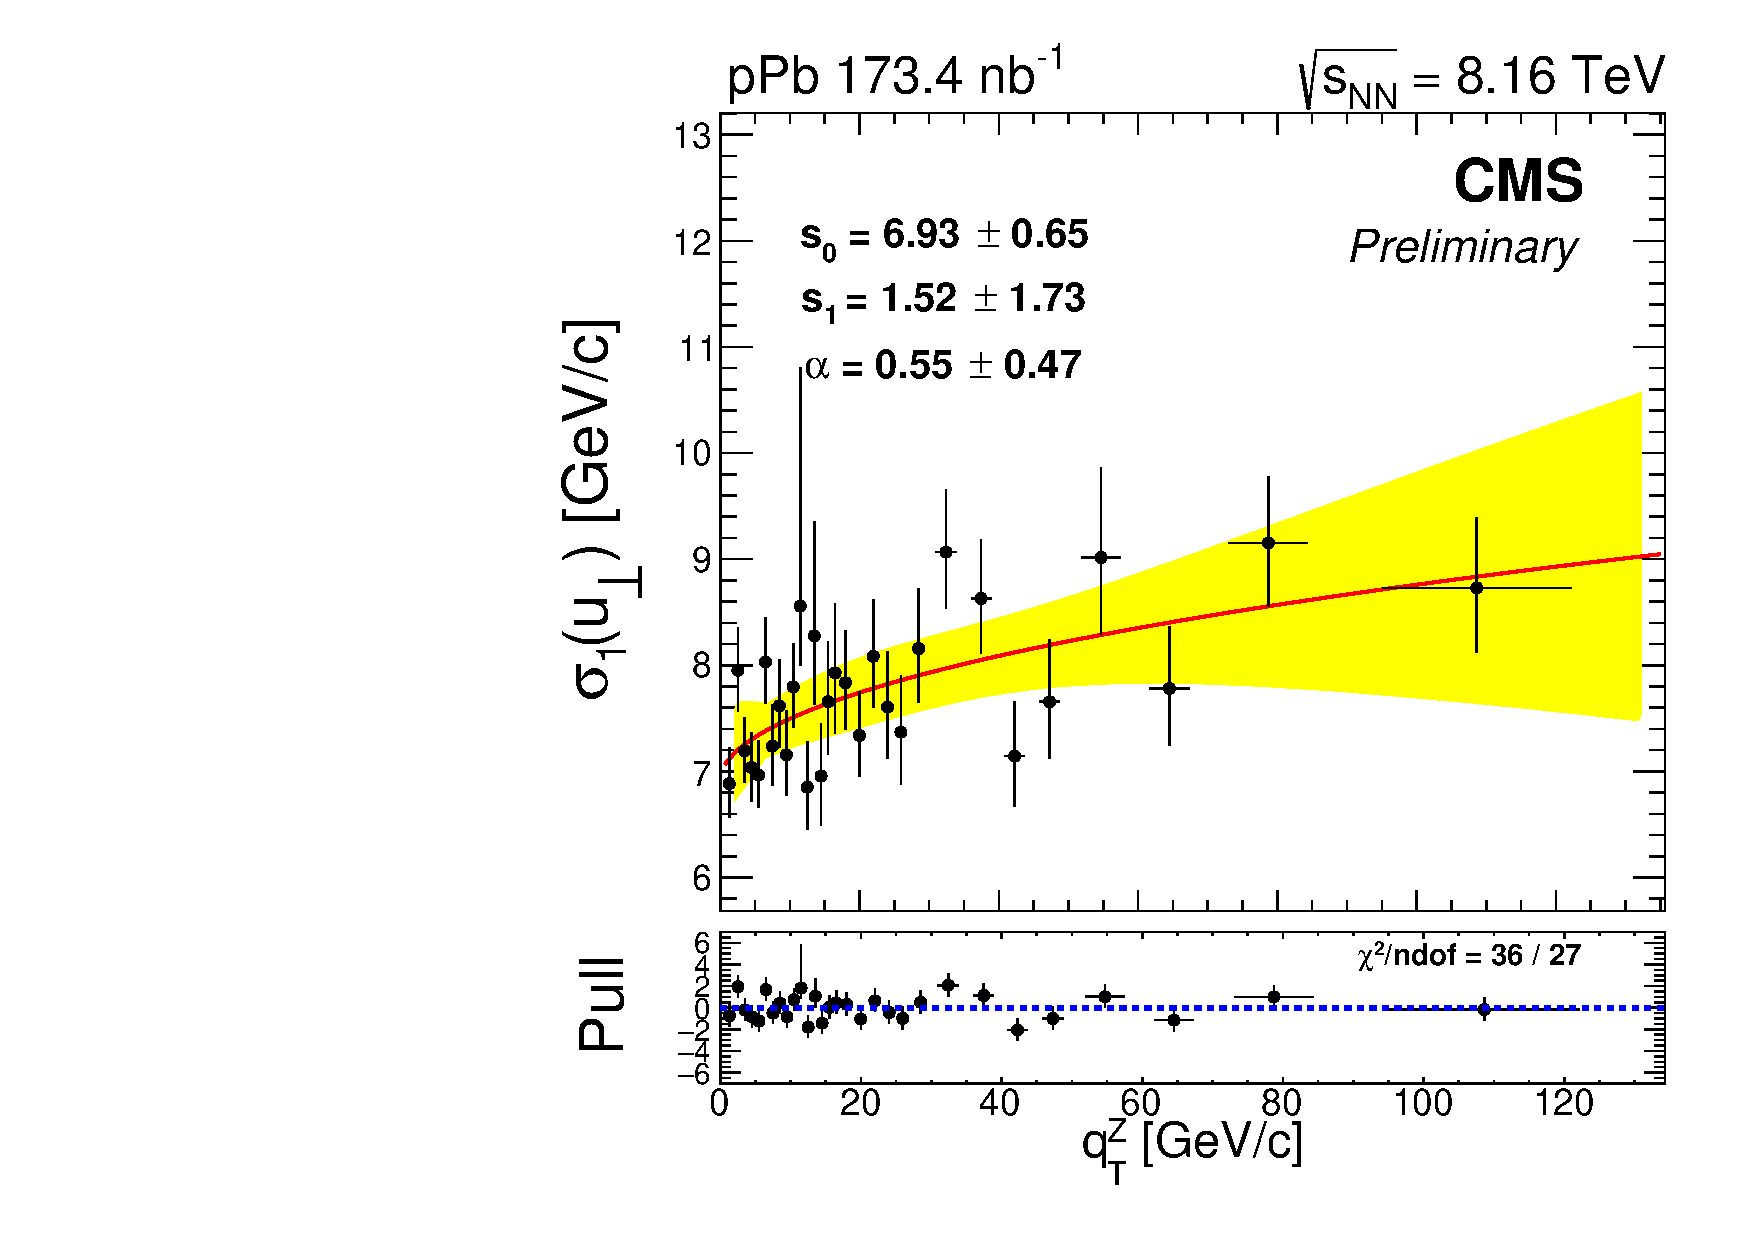
\includegraphics[width=0.3\textwidth]{Figures/WBoson/Analysis/Correction/Recoil/RecoilFitsqT/Data/fitPFu2sigma1.pdf}
  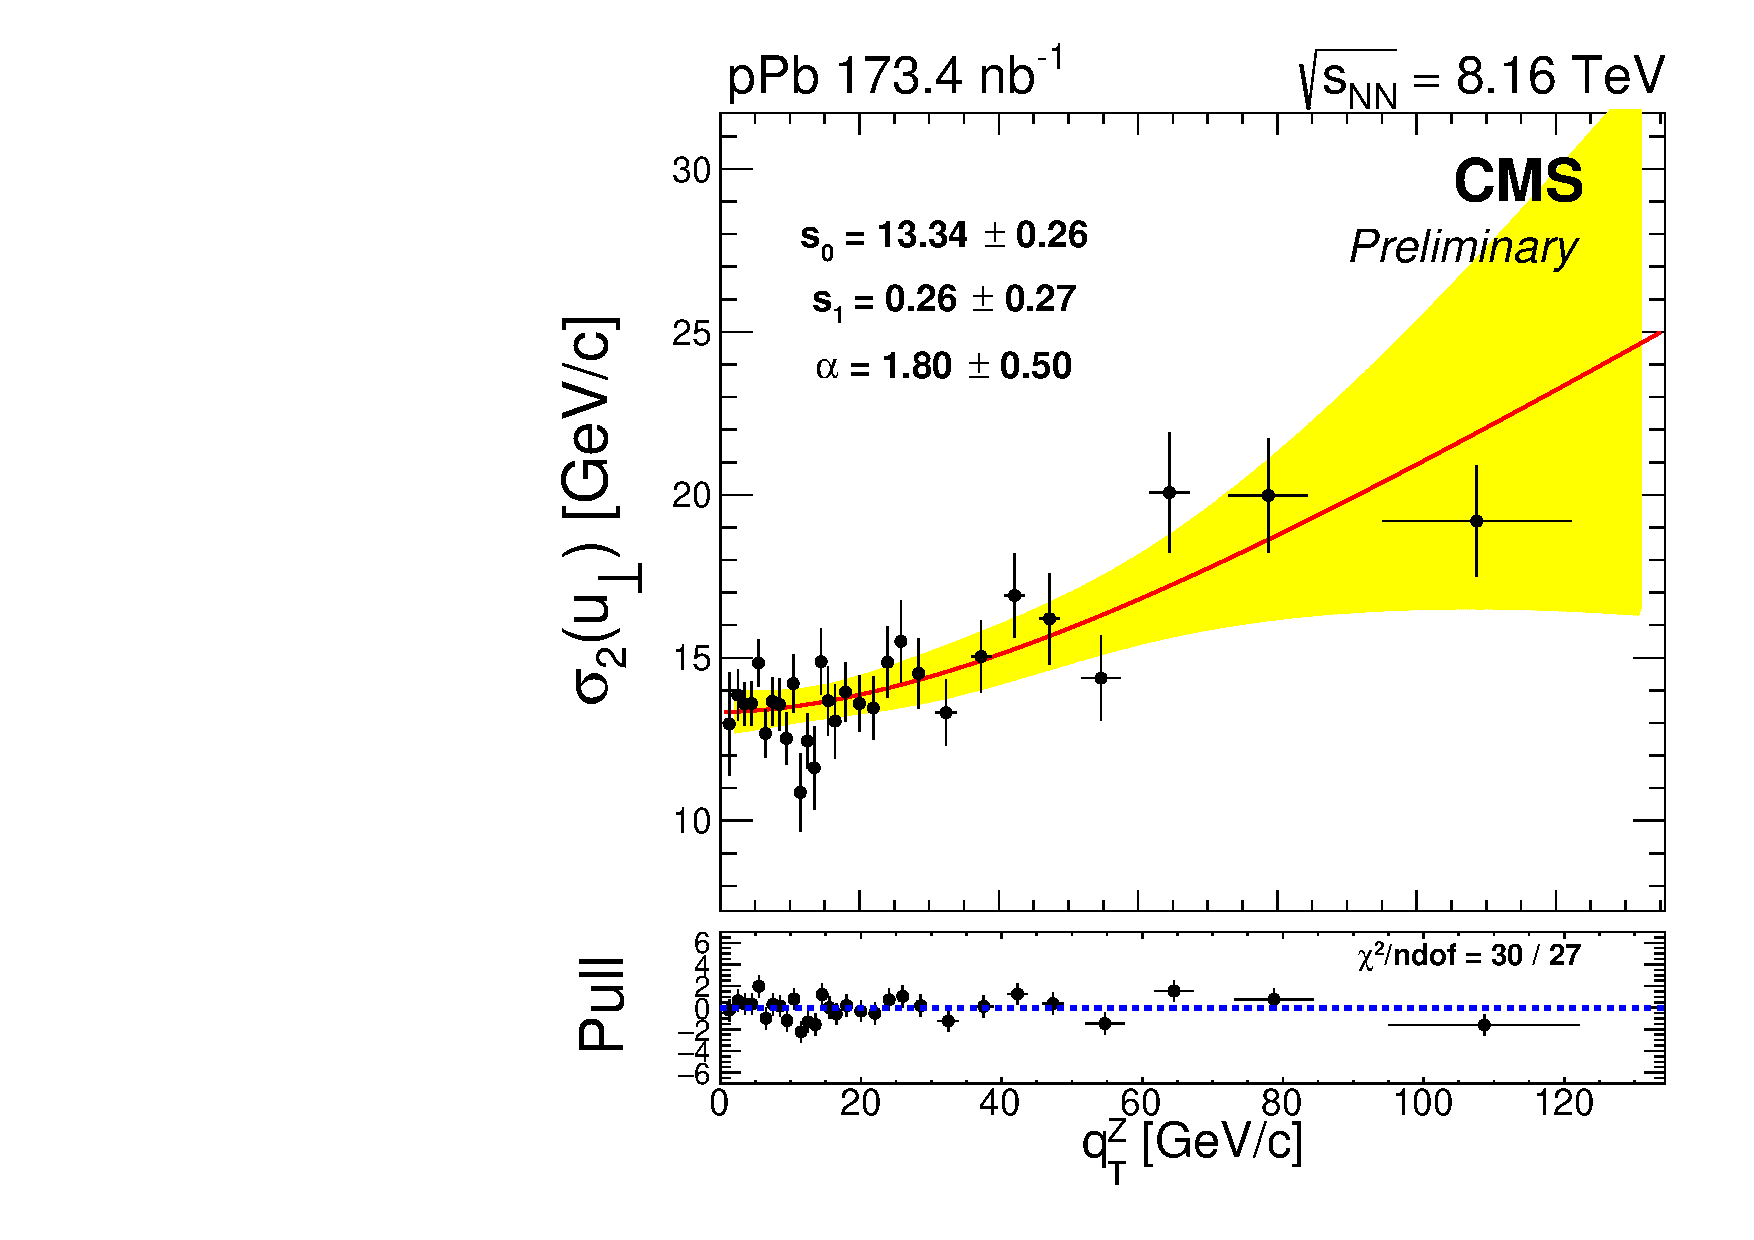
\includegraphics[width=0.3\textwidth]{Figures/WBoson/Analysis/Correction/Recoil/RecoilFitsqT/Data/fitPFu2sigma2.pdf}
  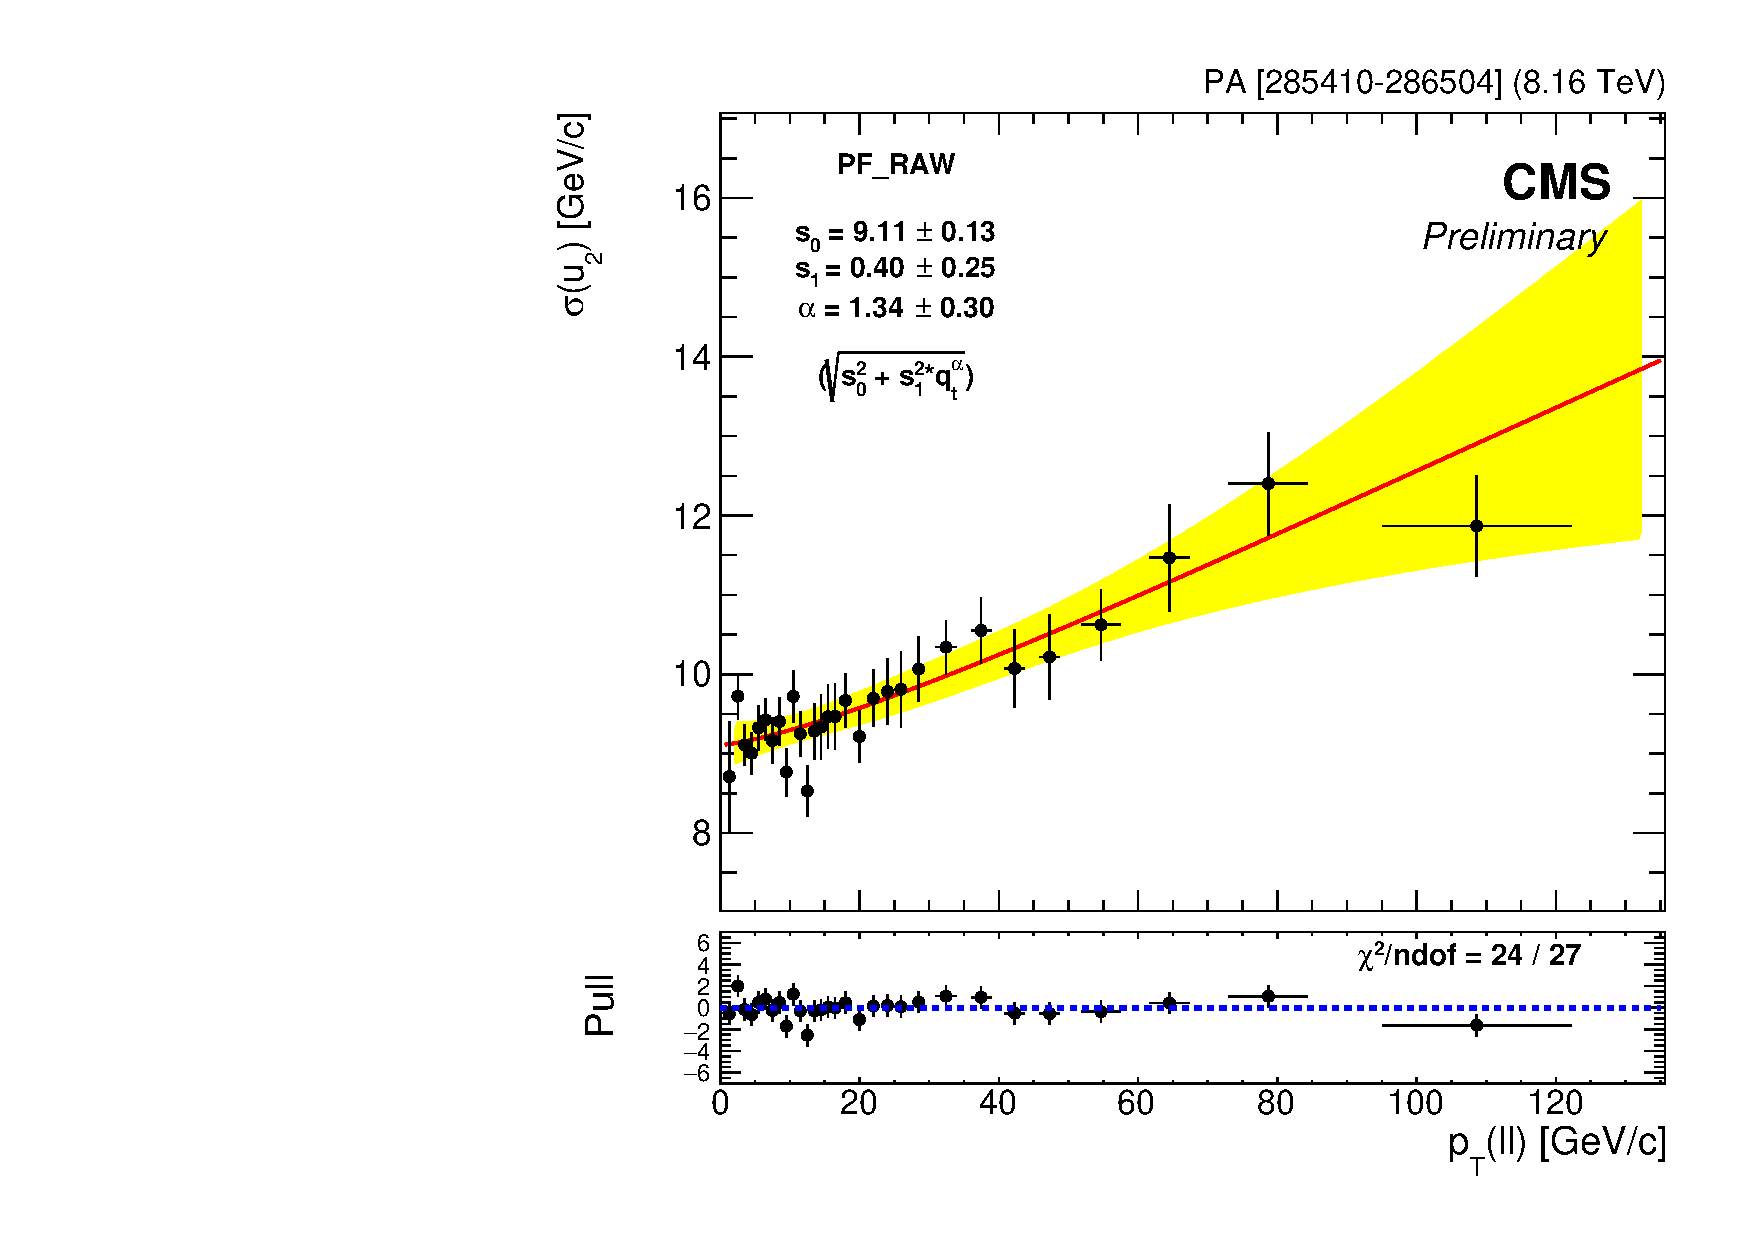
\includegraphics[width=0.3\textwidth]{Figures/WBoson/Analysis/Correction/Recoil/RecoilFitsqT/Data/fitPFu2sigma.pdf} \\
  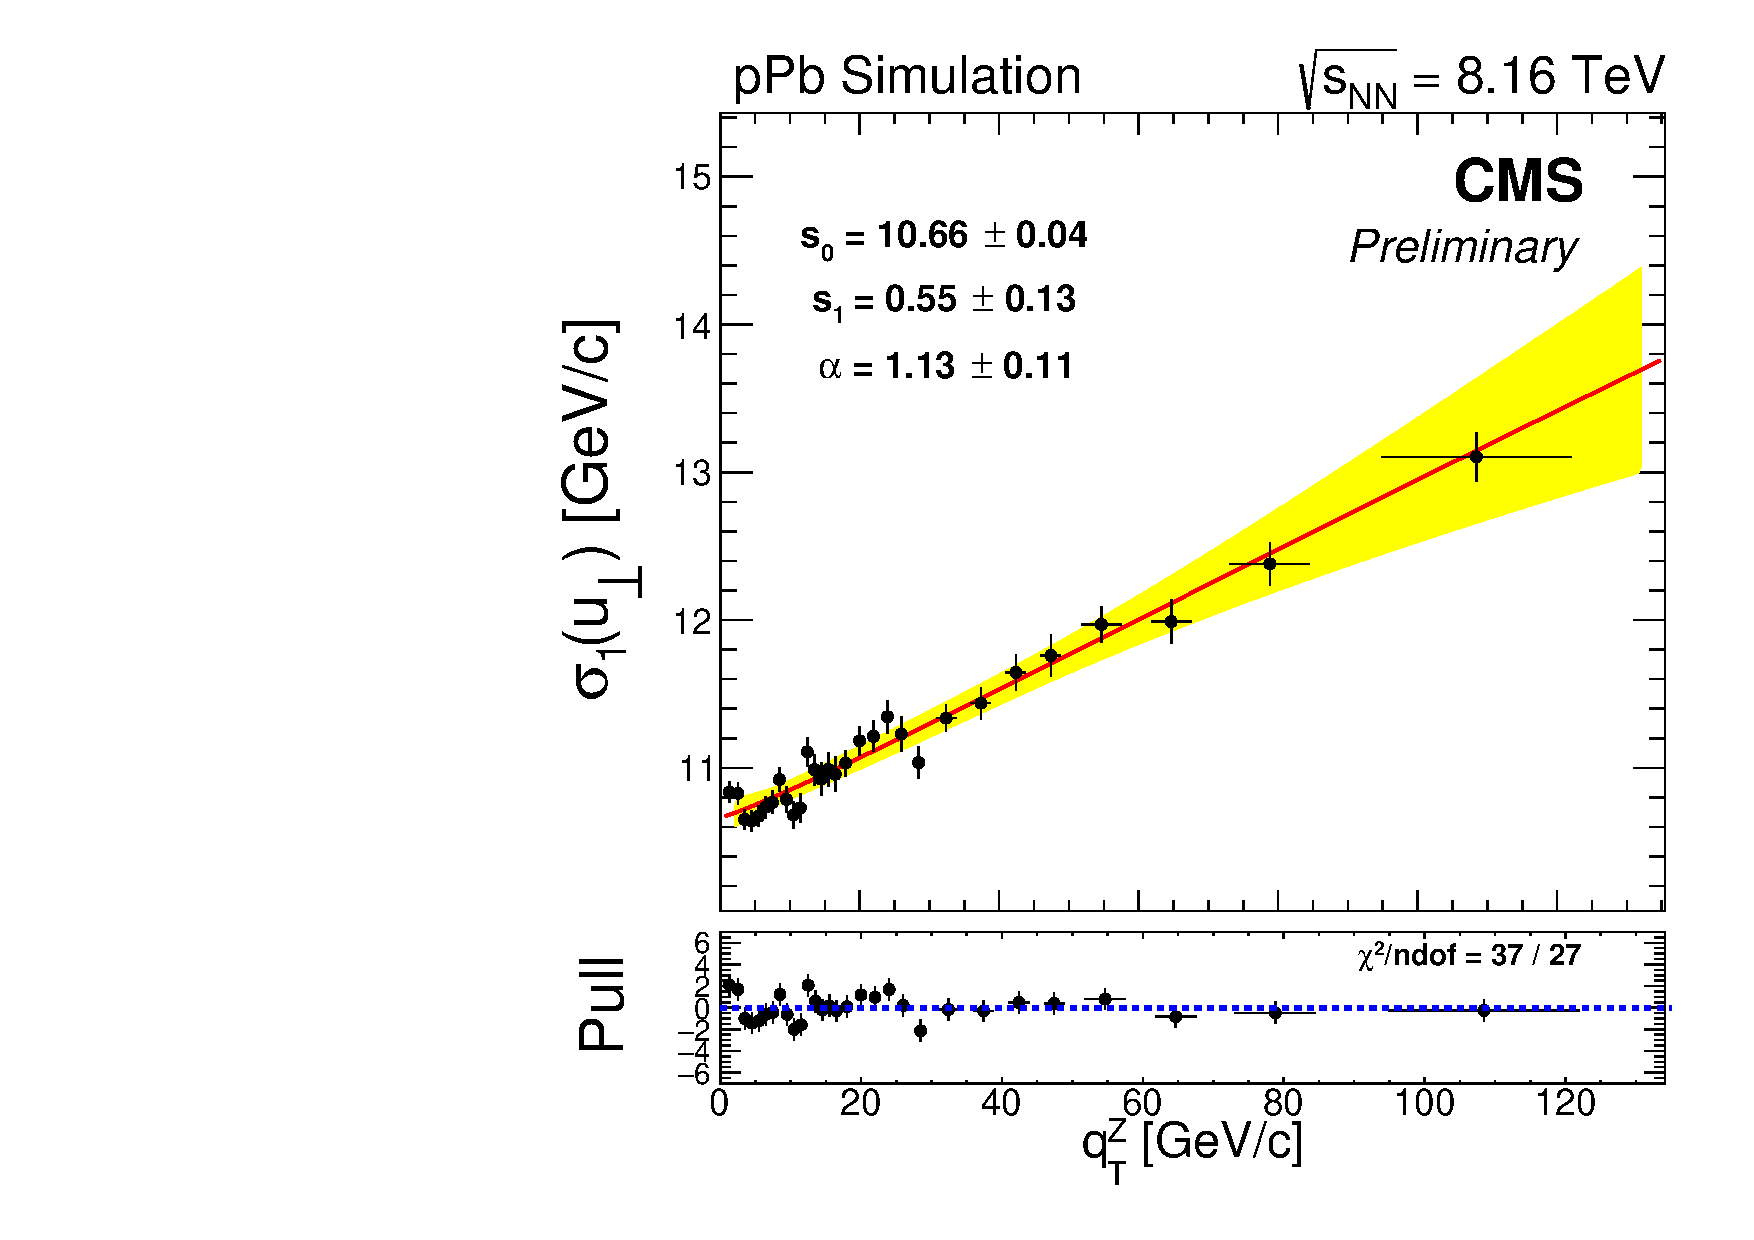
\includegraphics[width=0.3\textwidth]{Figures/WBoson/Analysis/Correction/Recoil/RecoilFitsqT/MC/fitPFu2sigma1.pdf}
  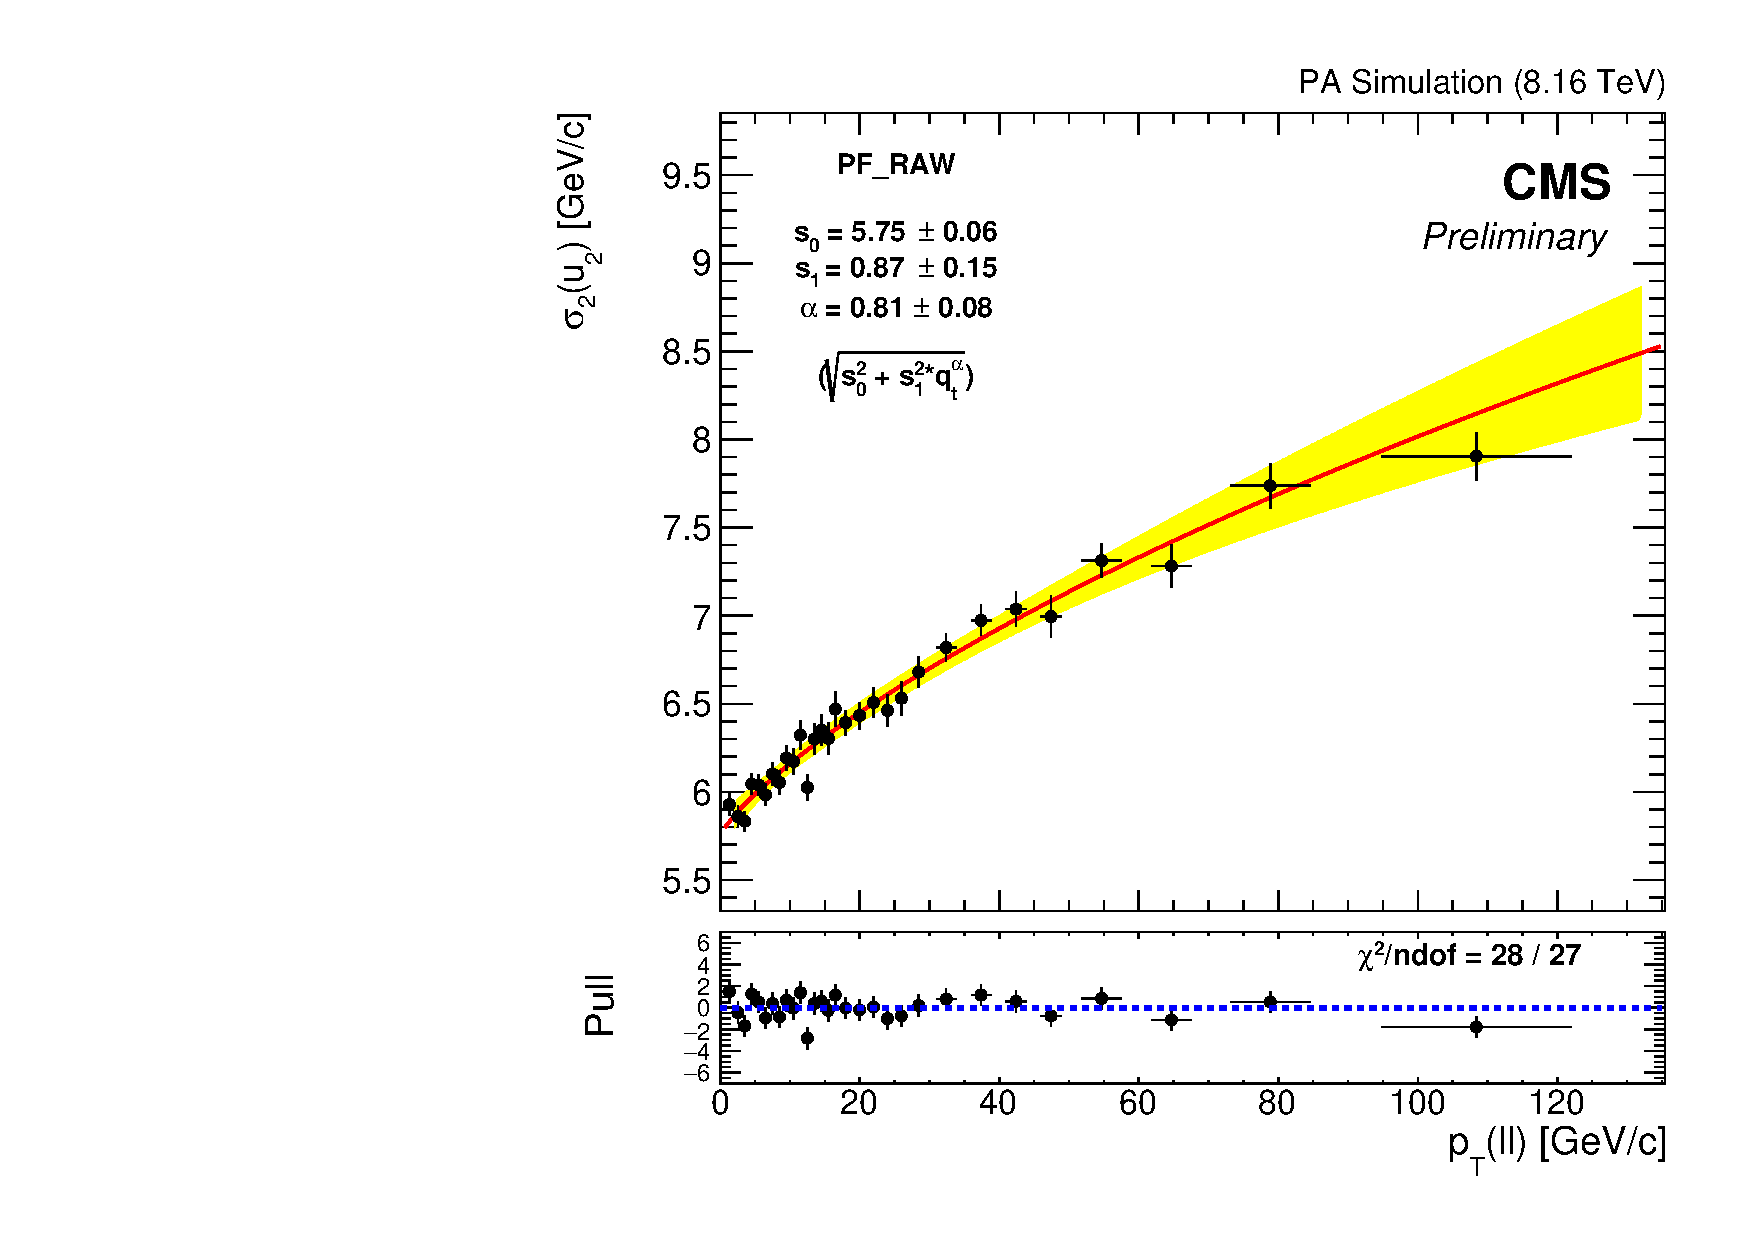
\includegraphics[width=0.3\textwidth]{Figures/WBoson/Analysis/Correction/Recoil/RecoilFitsqT/MC/fitPFu2sigma2.pdf}
  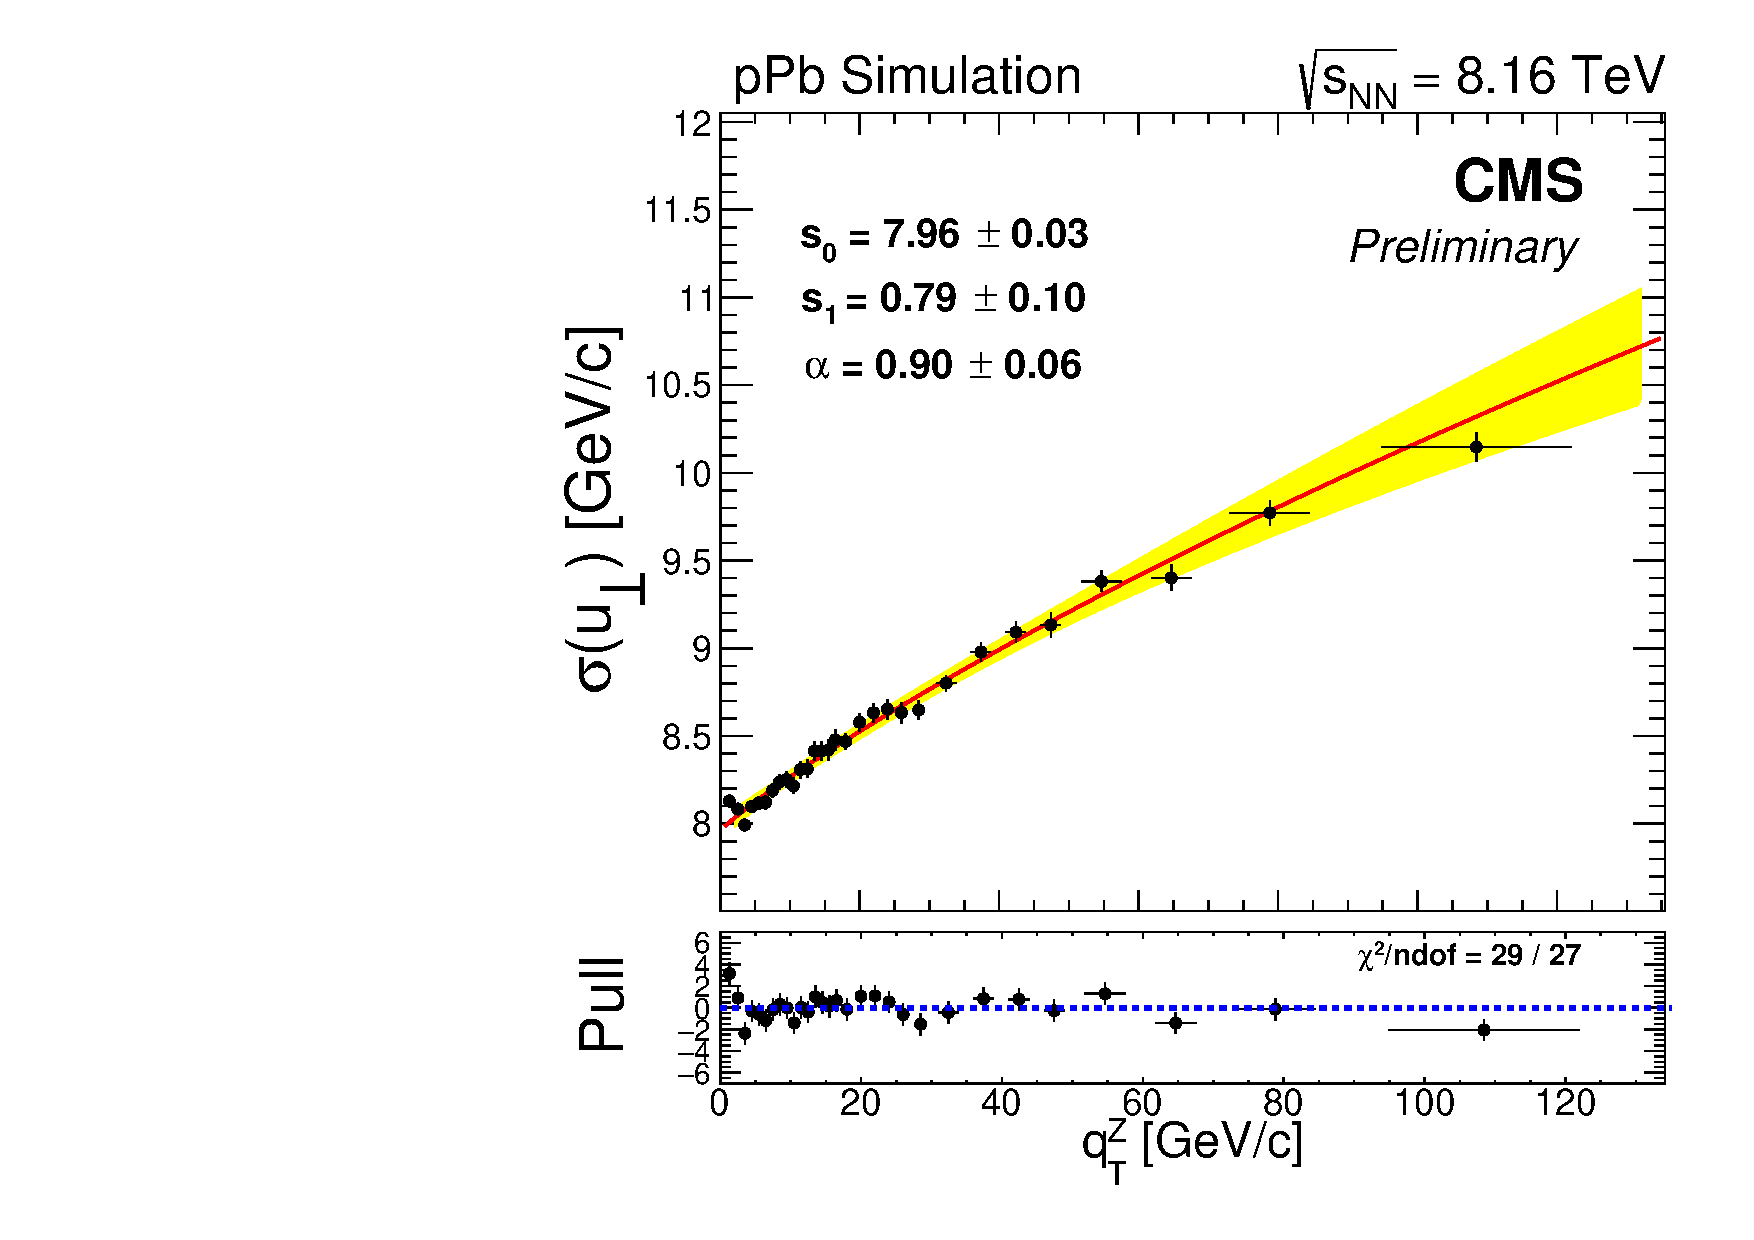
\includegraphics[width=0.3\textwidth]{Figures/WBoson/Analysis/Correction/Recoil/RecoilFitsqT/MC/fitPFu2sigma.pdf}
 \caption{Fits for the $\sigma_{1}$ (left), $\sigma_{2}$ (middle) and weighted average $\sigma$ (right) values of the recoil perpendicular component versus $q_{T}$. The plots on the top correspond to data while the plots in the bottom correspond to \ZToMuMu MC.}
 \label{fig:figU2RecoilResolutionFit}
 \end{center}
\end{figure}


\subsubsection{Recoil Correction}\label{sec:WBoson_Corrections_MET_RecoilCorr}

The simulated recoil distribution is corrected to match the scale and resolution observed in data. This can be done in two ways:

  \begin{itemize}
  \item Smearing method : Each component of the recoil distribution is smeared event-by-event using a gaussian probability distribution function defined as:
    \begin{equation}\label{eq:eqreccornsmrupar} 
%      u_{\parallel} = Gauss(u_{\parallel} - \tilde{u}_{\parallel}^{MC}(q_{T}) + \tilde{u}_{\parallel}^{data}(q_{T}), \sqrt{{\sigma_{\parallel}^{data}(q_{T},n)}^{2} - {\sigma_{\parallel}^{MC}(q_{T},n)}^{2}})
        u^{corr}_{\parallel} = Gauss(u_{\parallel} - \mu_{\parallel}^{MC}(q_{T}) + \mu_{\parallel}^{data}(q_{T}), \sqrt{{\sigma_{\parallel}^{data}(q_{T})}^{2} - {\sigma_{\parallel}^{MC}(q_{T})}^{2}}) \quad,
    \end{equation}
    \begin{equation}\label{eq:eqreccornsmruperp} 
        u^{corr}_{\perp} = Gauss(u_{\perp}, \sqrt{{\sigma_{\perp}^{data}(q_{T})}^{2} - {\sigma_{\perp}^{MC}(q_{T})}^{2}}) \quad,
    \end{equation}
    
    where $\mu$ and $\sigma$ are the weighted average values obtained in the previous subsections.
    
    \item Scaling method :  The parallel and perpendicular components of the simulated recoil are scaled in two possible ways:
    
      \begin{itemize}
       \item General case: Considering the full information of the double gaussian PDF used to fit the recoil distributions in data and MC, by using their Cumulative Distribution Functions (CDF).
       \begin{equation}\label{eq:eqRecCorrGeneralCase} 
         u^{corr}_{\parallel, \perp} = CDF^{-1}_{data}[CDF_{MC}[u_{\parallel, \perp}^{MC}]]
       \end{equation}
       
       \item Gaussian case: Approximating the recoil distributions by assuming a single gaussian PDF using the weighted average values $\mu$ and $\sigma$ derived before.
       \begin{equation}\label{eq:eqreccornsclupar} 
         u^{corr}_{\parallel} = (u_{\parallel} - \mu_{\parallel}^{MC}(q_{T}))\frac{\sigma_{\parallel}^{data}(q_{T})}{\sigma_{\parallel}^{MC}(q_{T})} + \mu_{\parallel}^{data}(q_{T}),
       \end{equation}
       \begin{equation}\label{eq:eqreccornscluperp} 
         u^{corr}_{\perp} = u_{\perp}\frac{\mu_{\perp}^{data}(q_{T})}{\sigma_{\perp}^{MC}(q_{T})}
       \end{equation}
      \end{itemize}

  \end{itemize}

Once the recoil is corrected, the MET distribution is recalculated as:

\begin{equation}
 \textsc{MET}_{corr} = \left|\vec{p}^{\mu}_{T} + \vec{u}_{corr}\right|
\end{equation}


\subsubsection{Recoil Correction: Control Region}\label{sec:WBoson_Corrections_MET_closureTests}

The recoil corrections are checked by applying them on the same MC sample used to derive the recoil corrections (Z boson enriched). The data and simulation (including HF reweighing) corrected MET distributions are shown in \fig{fig:recoilClosure} in the inclusive (left) and in a selected (right) pseudorapidity region. As can be observed, the  agreement between simulation and data is greatly improved after applying the recoil correction using the gaussian scaling method.

\begin{figure}[!h]
 \begin{center}
  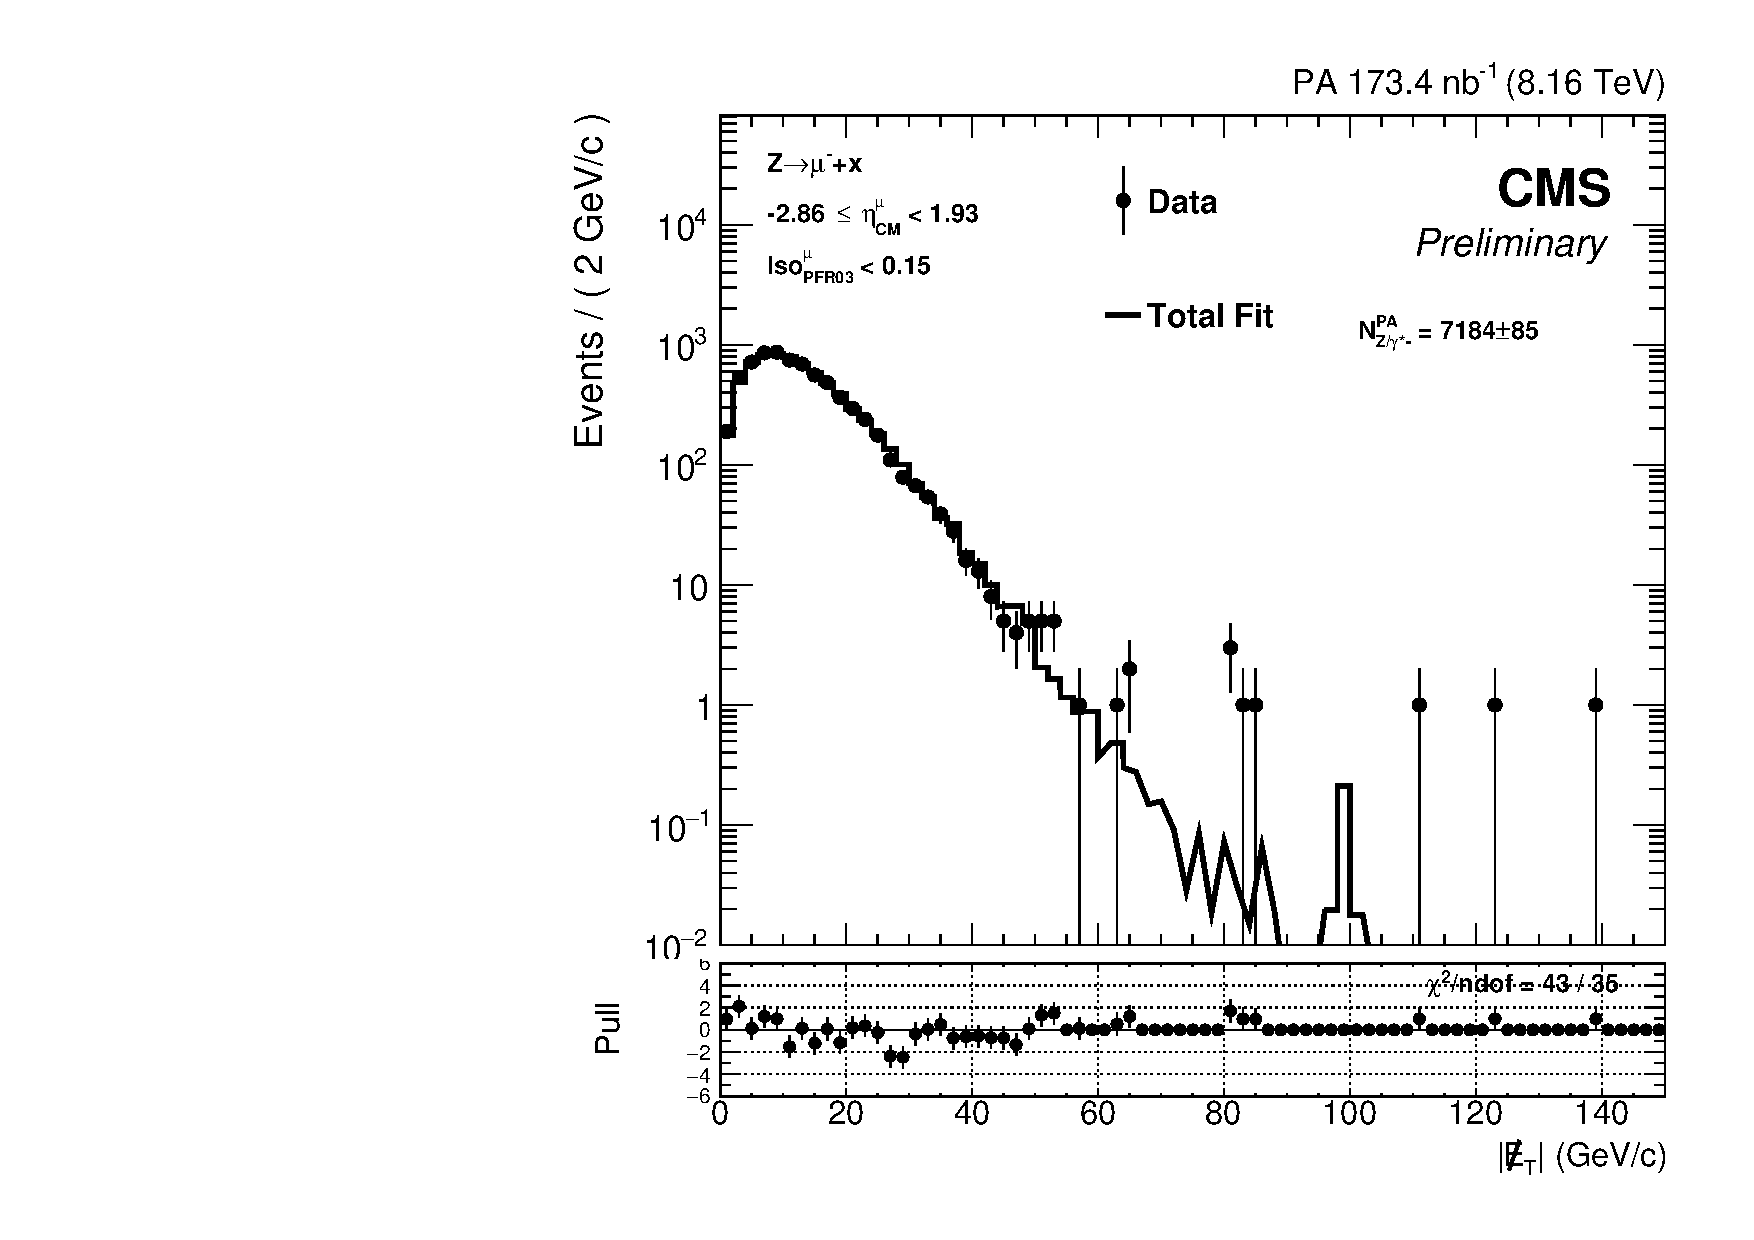
\includegraphics[width=0.4\textwidth]{Figures/WBoson/Analysis/Correction/Recoil/CheckFits/Z/Recoil_ScalingGauss/PLOT_MET_DATA_ZToMuMi_PA_Model_TEMP_DY_MuEtaCM_m286_193_MuIso_0_15.pdf}
  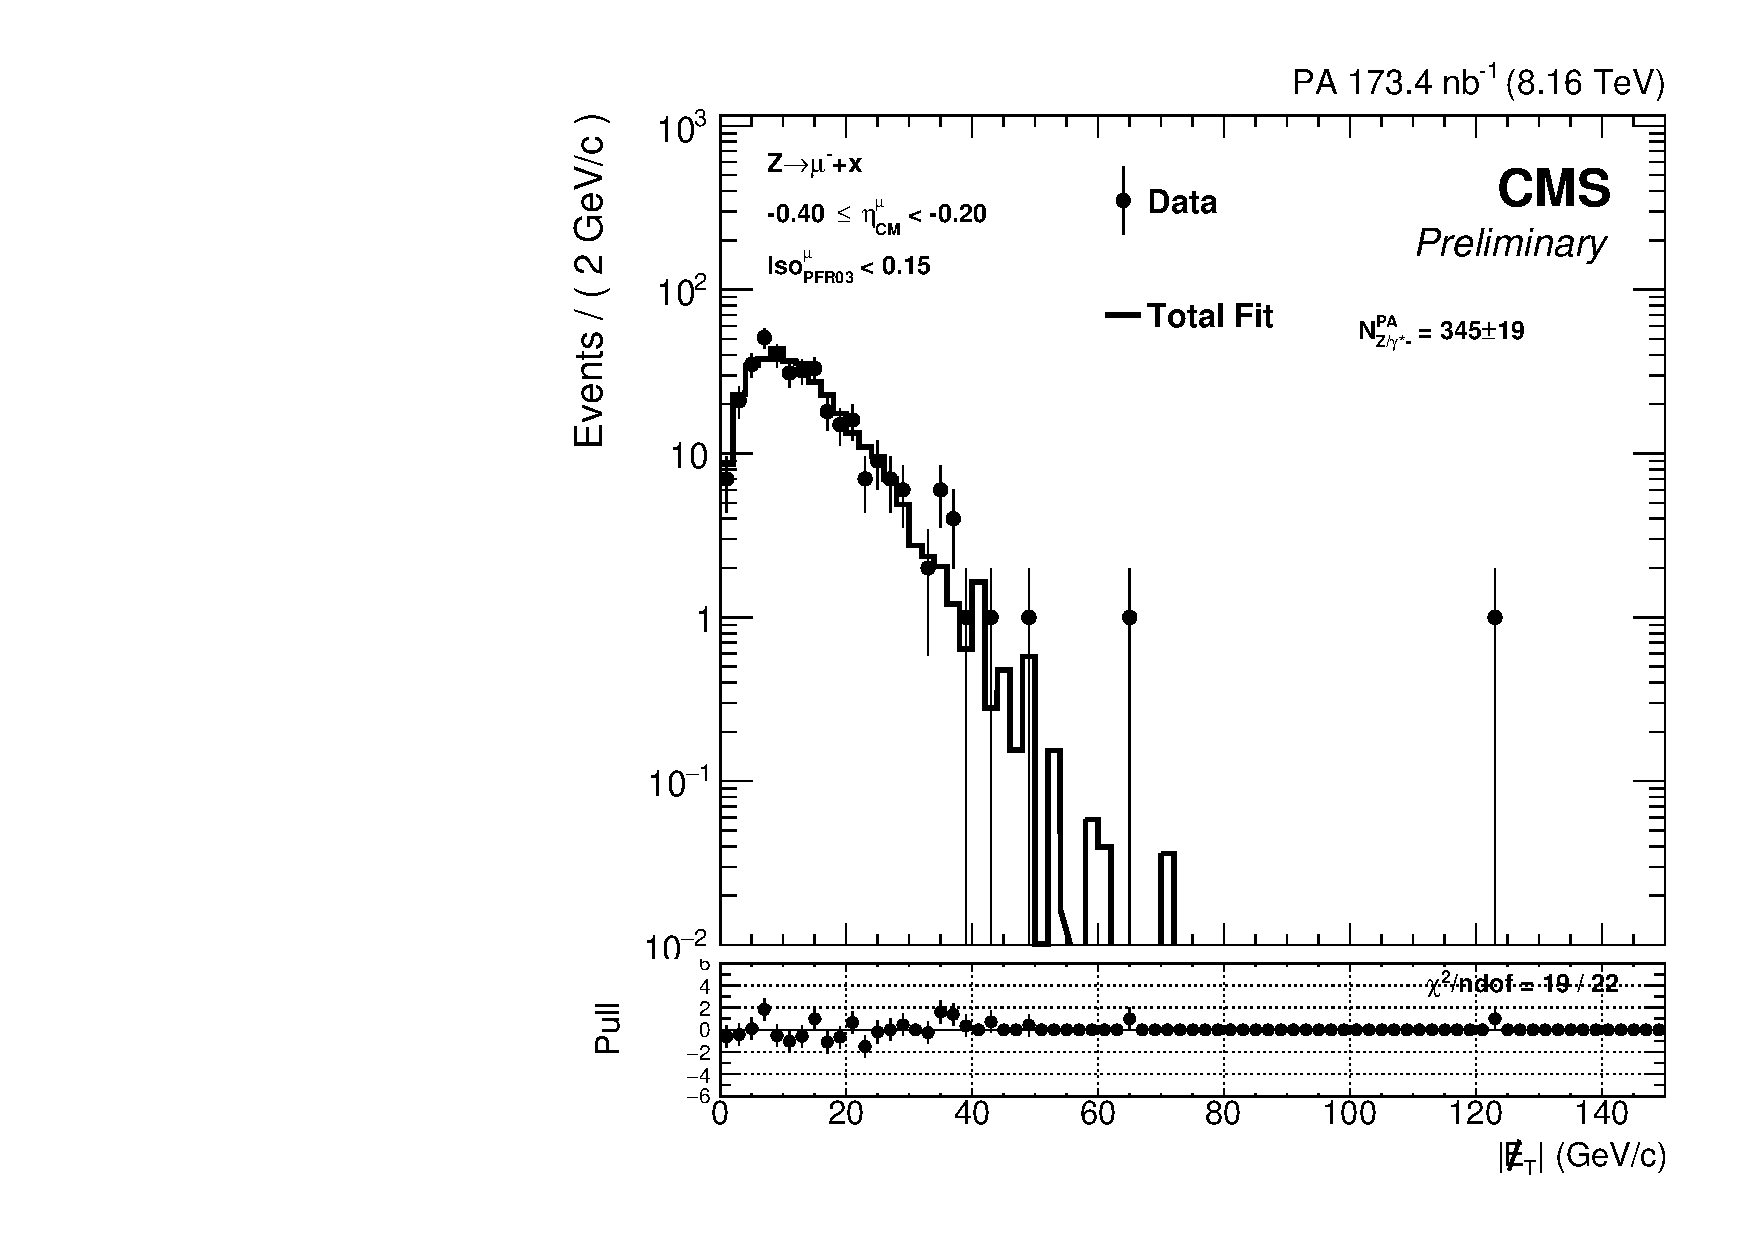
\includegraphics[width=0.4\textwidth]{Figures/WBoson/Analysis/Correction/Recoil/CheckFits/Z/Recoil_ScalingGauss/PLOT_MET_DATA_ZToMuMi_PA_Model_TEMP_DY_MuEtaCM_m40_m20_MuIso_0_15.pdf} 
  \caption{A comparison of the MET distribution in data and MC for Z boson selected events. The left plot corresponds to the full pseudorapidity range in the analysis while the right one corresponds to an pecific pseudorapidity bin. The recoil correction using the gaussian scaling method has been applied to MC.}
 \label{fig:recoilClosure}
 \end{center}
\end{figure}

\subsubsection{Recoil Correction: Signal Region}\label{sec:WBoson_Corrections_MET_RecoilSignal}

The \W signal in data is extracted following the procedure in \sect{sec:WBoson_SignalExtraction}. The recoil corrections are applied to the \W boson MC using the 3 methods detailed in \sect{sec:WBoson_Corrections_MET_RecoilCorr}, in order to determine which one works better. \fig{fig:recoilCorrWreg} shows the data fits in the \W region with the scaling method in the general case (left), gaussian case (middle) and the smearing method (right), for the full pseudorapidity region used in the analysis. The gaussian scaling provides the best fits, so it is used as nominal correction method.

\begin{figure}[!h]
 \begin{center}
  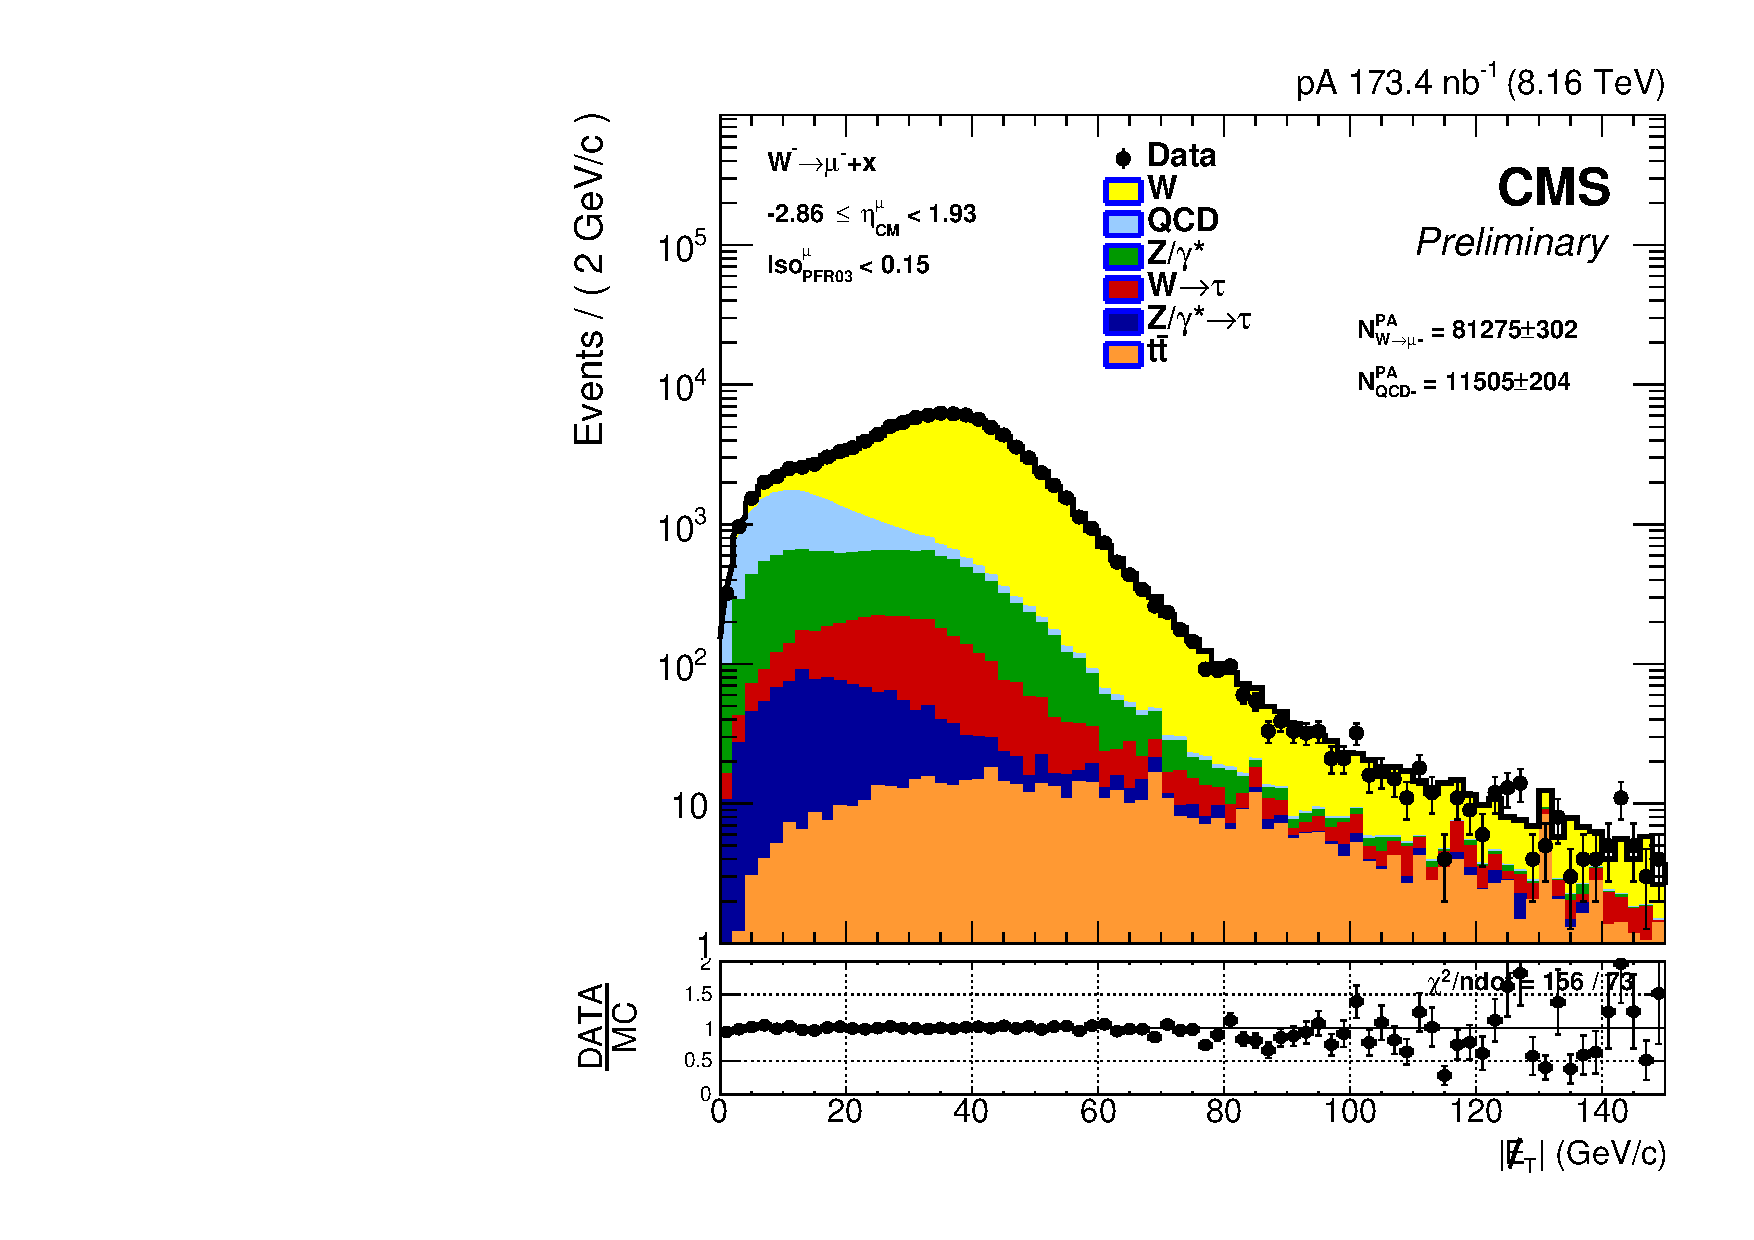
\includegraphics[width=0.3\textwidth]{Figures/WBoson/Analysis/Correction/Recoil/CheckFits/W/Recoil_ScalingGeneral/PLOT_MET_DATA_WToMuMi_PA_Model_TEMP_WDYDYToTauWToTauTTbar_ModifiedRayleigh_QCD_MuEtaCM_m286_193_MuIso_0_15.pdf}
  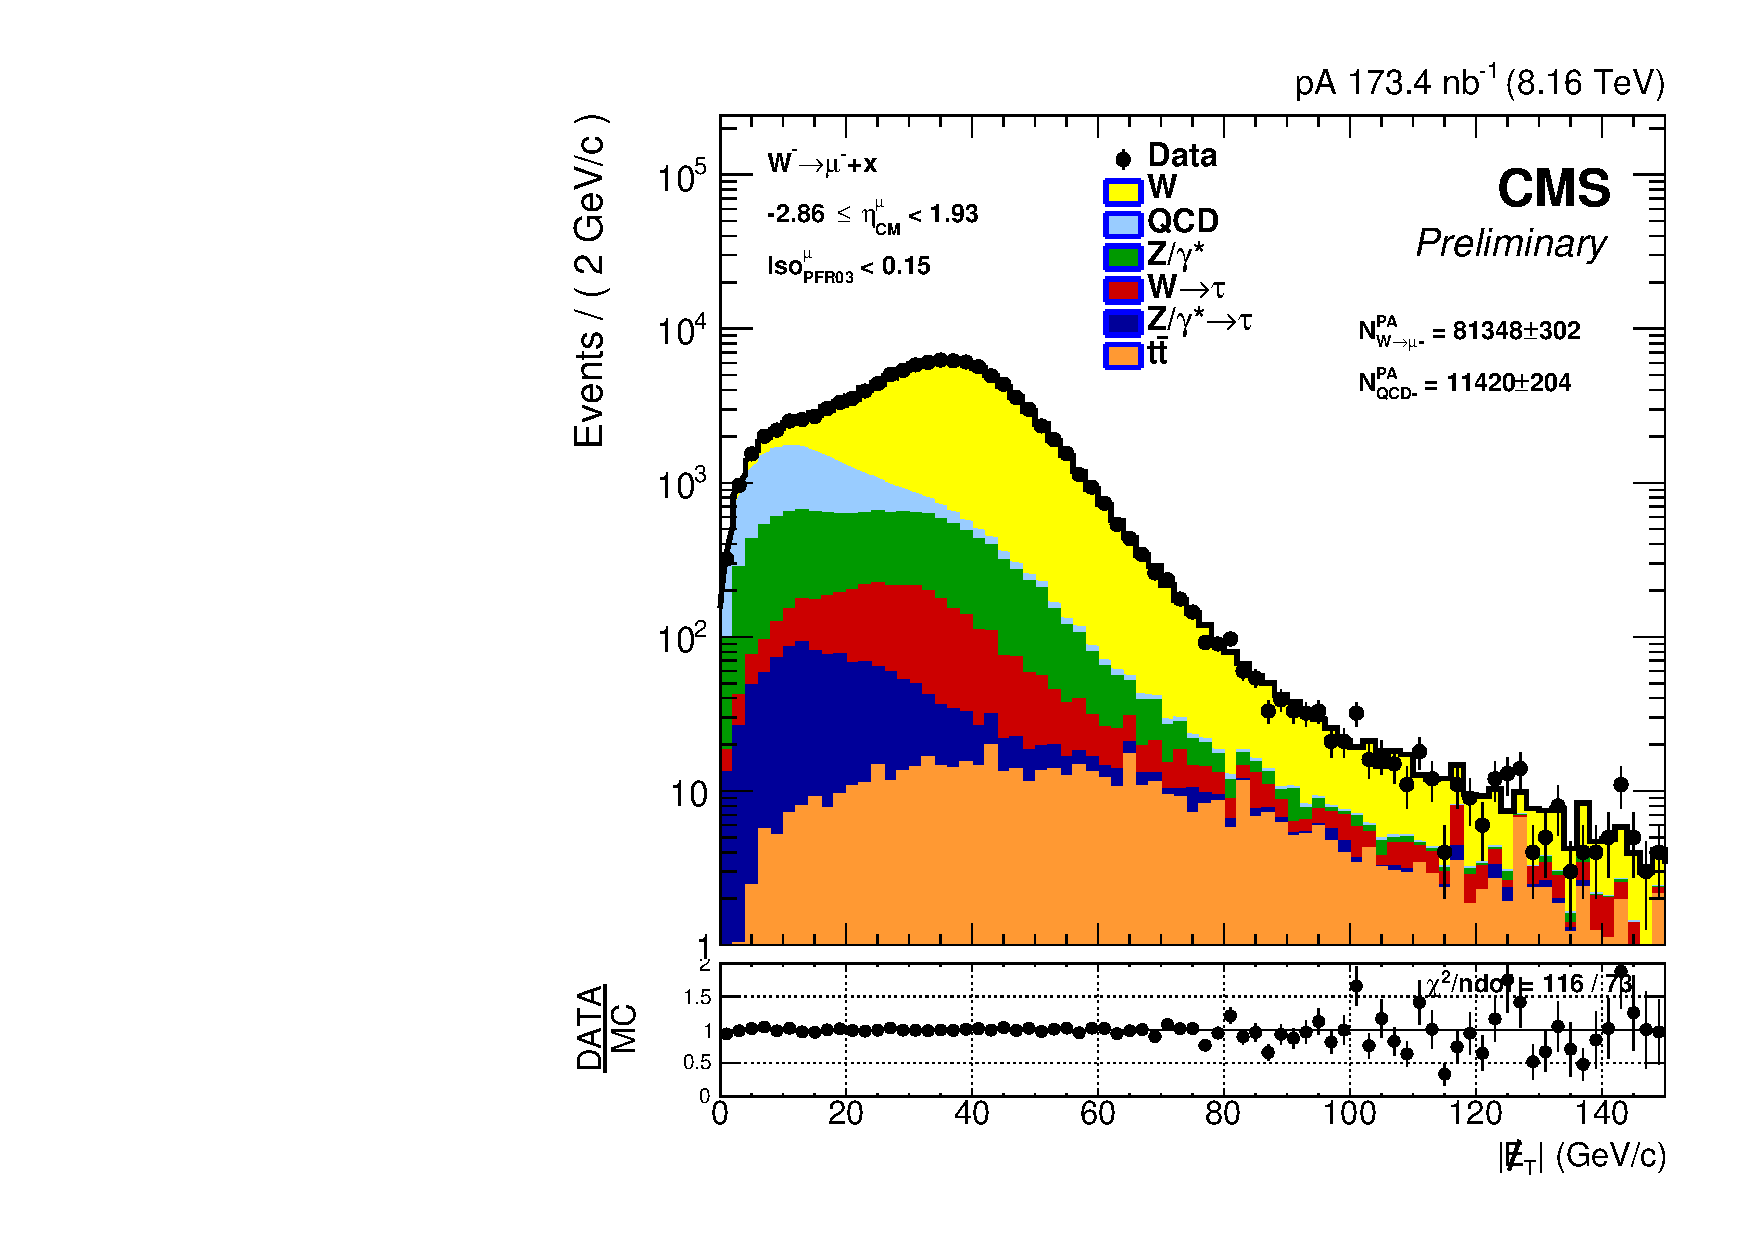
\includegraphics[width=0.3\textwidth]{Figures/WBoson/Analysis/Correction/Recoil/CheckFits/W/Recoil_ScalingGauss/PLOT_MET_DATA_WToMuMi_PA_Model_TEMP_WDYDYToTauWToTauTTbar_ModifiedRayleigh_QCD_MuEtaCM_m286_193_MuIso_0_15.pdf}
  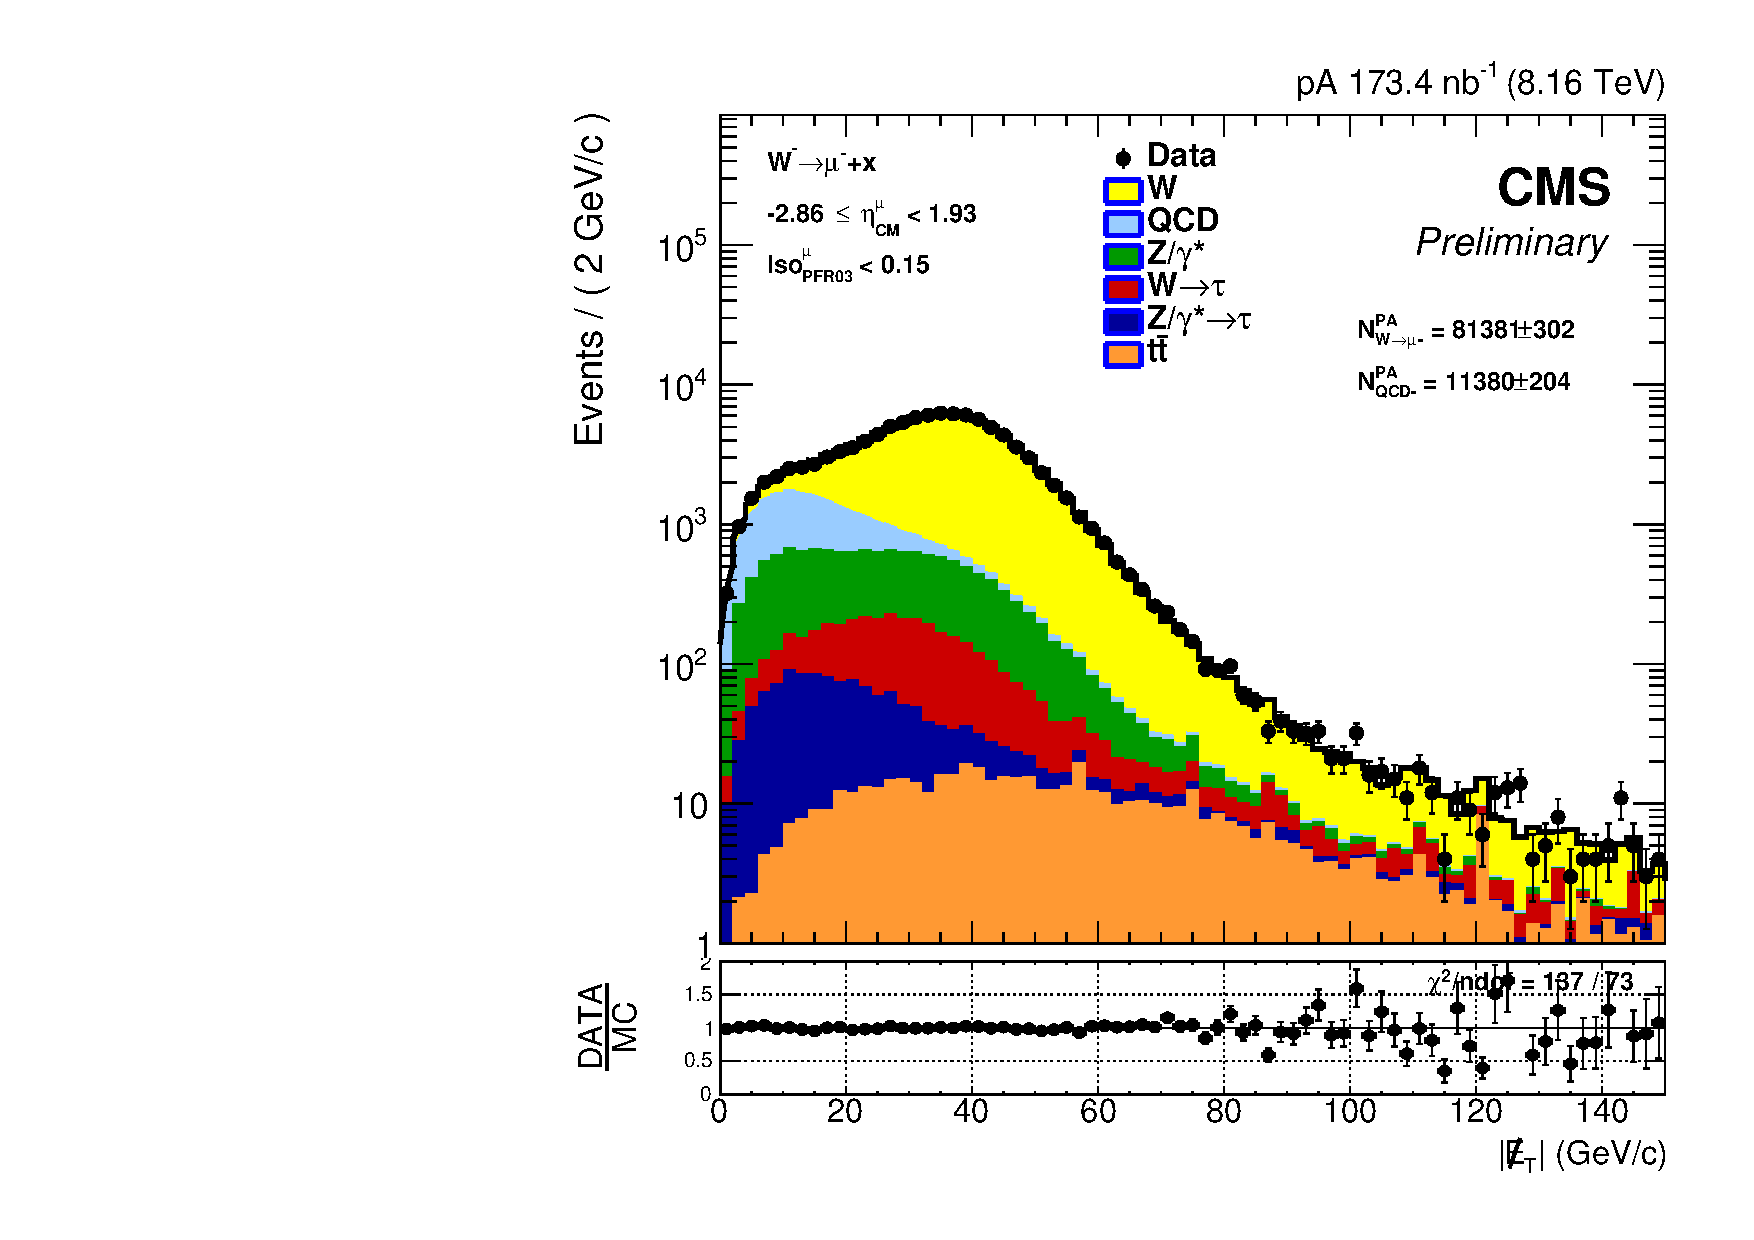
\includegraphics[width=0.3\textwidth]{Figures/WBoson/Analysis/Correction/Recoil/CheckFits/W/Recoil_Smearing/PLOT_MET_DATA_WToMuMi_PA_Model_TEMP_WDYDYToTauWToTauTTbar_ModifiedRayleigh_QCD_MuEtaCM_m286_193_MuIso_0_15.pdf}
  \caption{A comparison of the MET distribution in data and MC for W boson selected events in the full pseudorapidity range in the analysis. Different methods to apply the recoil corrections in MC are used in each plot. The left plot corresponds to the scaling method in the general case, the middle one corresponds to the scaling method in the gaussian case, and the right one to the smearing method.}
 \end{center}
 \label{fig:recoilCorrWreg}
\end{figure}


% END OF SUBSECTION


\section{Signal efficiency}\label{sec:WBoson_Efficiency}

The signal truth efficiency is estimated using the \WToMuNu\ NLO MC samples since they contain the full history of the events, including the generation and reconstruction of the particles. The energy deposited in the HF calorimeters is reweighed in MC to match the distribution observed in data as explained in \sect{sec:WBoson_Corrections_EventActivityReweighing}.

A reconstructed muon is considered an offline muon if it passes all the \W boson analysis cuts detailed in \sect{sec:WBoson_Selection_WSelection}. Among the selection criteria, an offline muon is required to pass the isolation and tight identification cuts defined in \sect{sec:WBoson_Selection_MuonIdentification}, be trigger matched, and have a $\pt~>~25$~\GeVc and $|\eta|~<~2.4$.

The muon truth efficiency is defined as the fraction of generated muons matched to an offline muon around a cone of $\Delta{R} < 0.05$.  All the generated muons are required to be inside the analysis kinematic region ($\pt~>~25$~\GeVc and $|\eta|~<~2.4$) and come from a \W boson decay. The muon truth efficiency is described in \eq{eq:MCTruthEfficiency}.

\begin{equation}
\epsilon^{\mu^{\pm}}_{offline}(p_{T}^{gen} , \eta^{gen}) = \frac{N_{gen,\pt>25}^{\mu^{\pm}}(p_{T}^{gen} , \eta^{gen})[\textnormal{Matched to }\mu_{offline}^{\pm}]}{N_{gen,\pt>25}^{\mu^{\pm}}(p_{T}^{gen} , \eta^{gen})}
\label{eq:MCTruthEfficiency}
\end{equation}

The muon efficiencies of the \RunpPb and \RunPbp MC samples are calculated individually and later combined following the strategy described in \sect{sec:WBoson_Sample_CombiningBeamDirection}. After flipping the sign of the muon $\eta_{LAB}$ in the \RunPbp sample, the combined efficiency is determined as presented in \eq{eq:MCEfficiencyPA}, by taking into account the corresponding recorded integrated luminosities of each run (see \sect{sec:WBoson_Samples_Data}). The combined efficiency is labelled as pA muon efficiency.

\begin{equation}
\epsilon^{\mu^{\pm}}_{PA}(p_{T}^{gen} , \eta^{gen}) = \frac{\sigma^{MC}_{\pPb}\times\Lumi_{\pPb}\times\epsilon^{\mu^{\pm}}_{\pPb}(p_{T}^{gen} , \eta^{gen}) + \sigma^{MC}_{\Pbp}\times\Lumi_{\Pbp}\times\epsilon^{\mu^{\pm}}_{\Pbp}(p_{T}^{gen} , -\eta^{gen})}{\sigma^{MC}_{\pPb}\times\Lumi_{\pPb} + \sigma^{MC}_{\Pbp}\times\Lumi_{\Pbp}}
\label{eq:MCEfficiencyPA}
\end{equation}

The statistical uncertainty of the muon efficiencies is determined using the ROOT class TEfficiency \cite{ROOT}. The uncertainty is estimated by applying Bayesian statistics using a Jeffrey's prior and considering a 68$\%$ credible interval. The results of the \WToMuNu truth efficiency extracted from the combined pA MC samples are shown in \fig{fig:MCTruthEfficiency}.

\begin{figure}[htb!]
 \begin{center}
   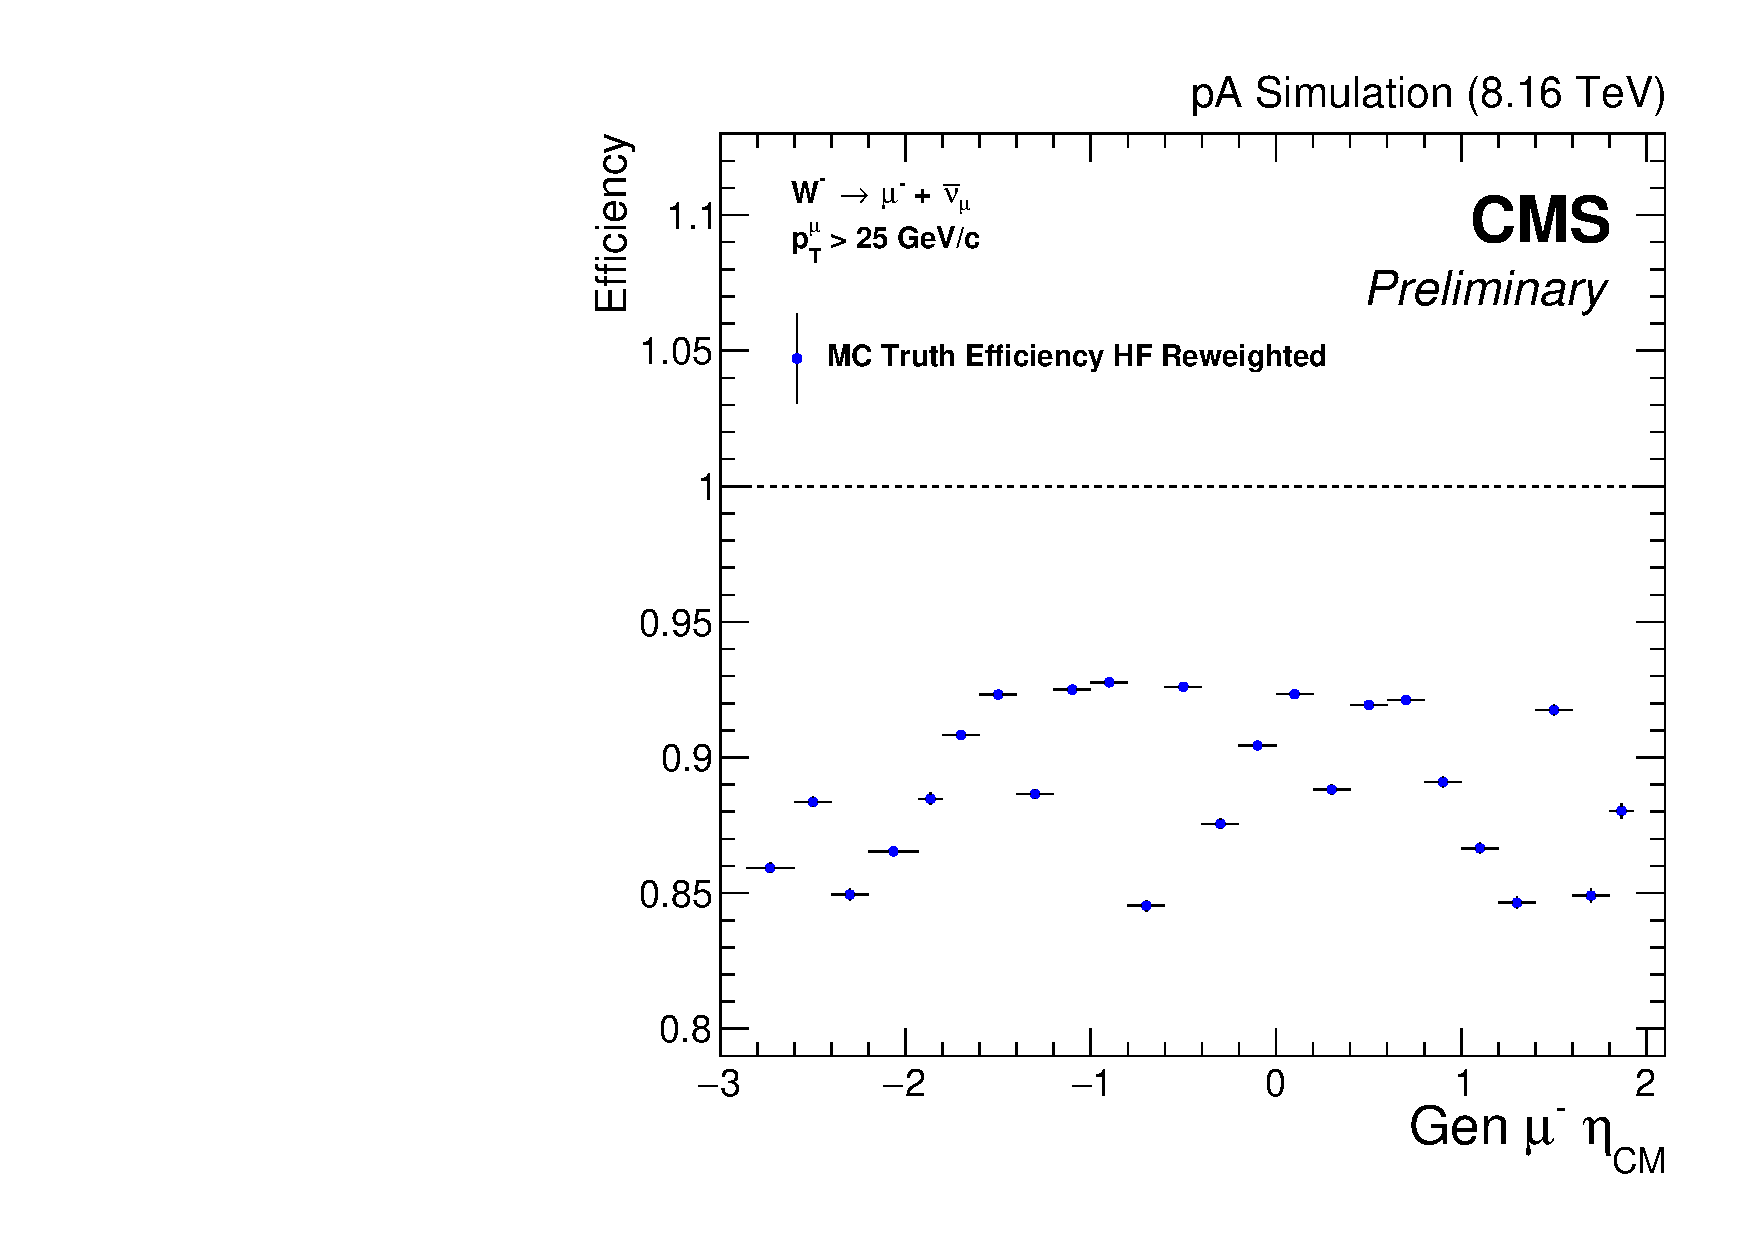
\includegraphics[width=0.45\textwidth]{Figures/WBoson/Analysis/Efficiency/Muon/PA/eff1D_EtaCM_MC_WToMuNu_PA_Minus_Total_HFCorrOnly}
   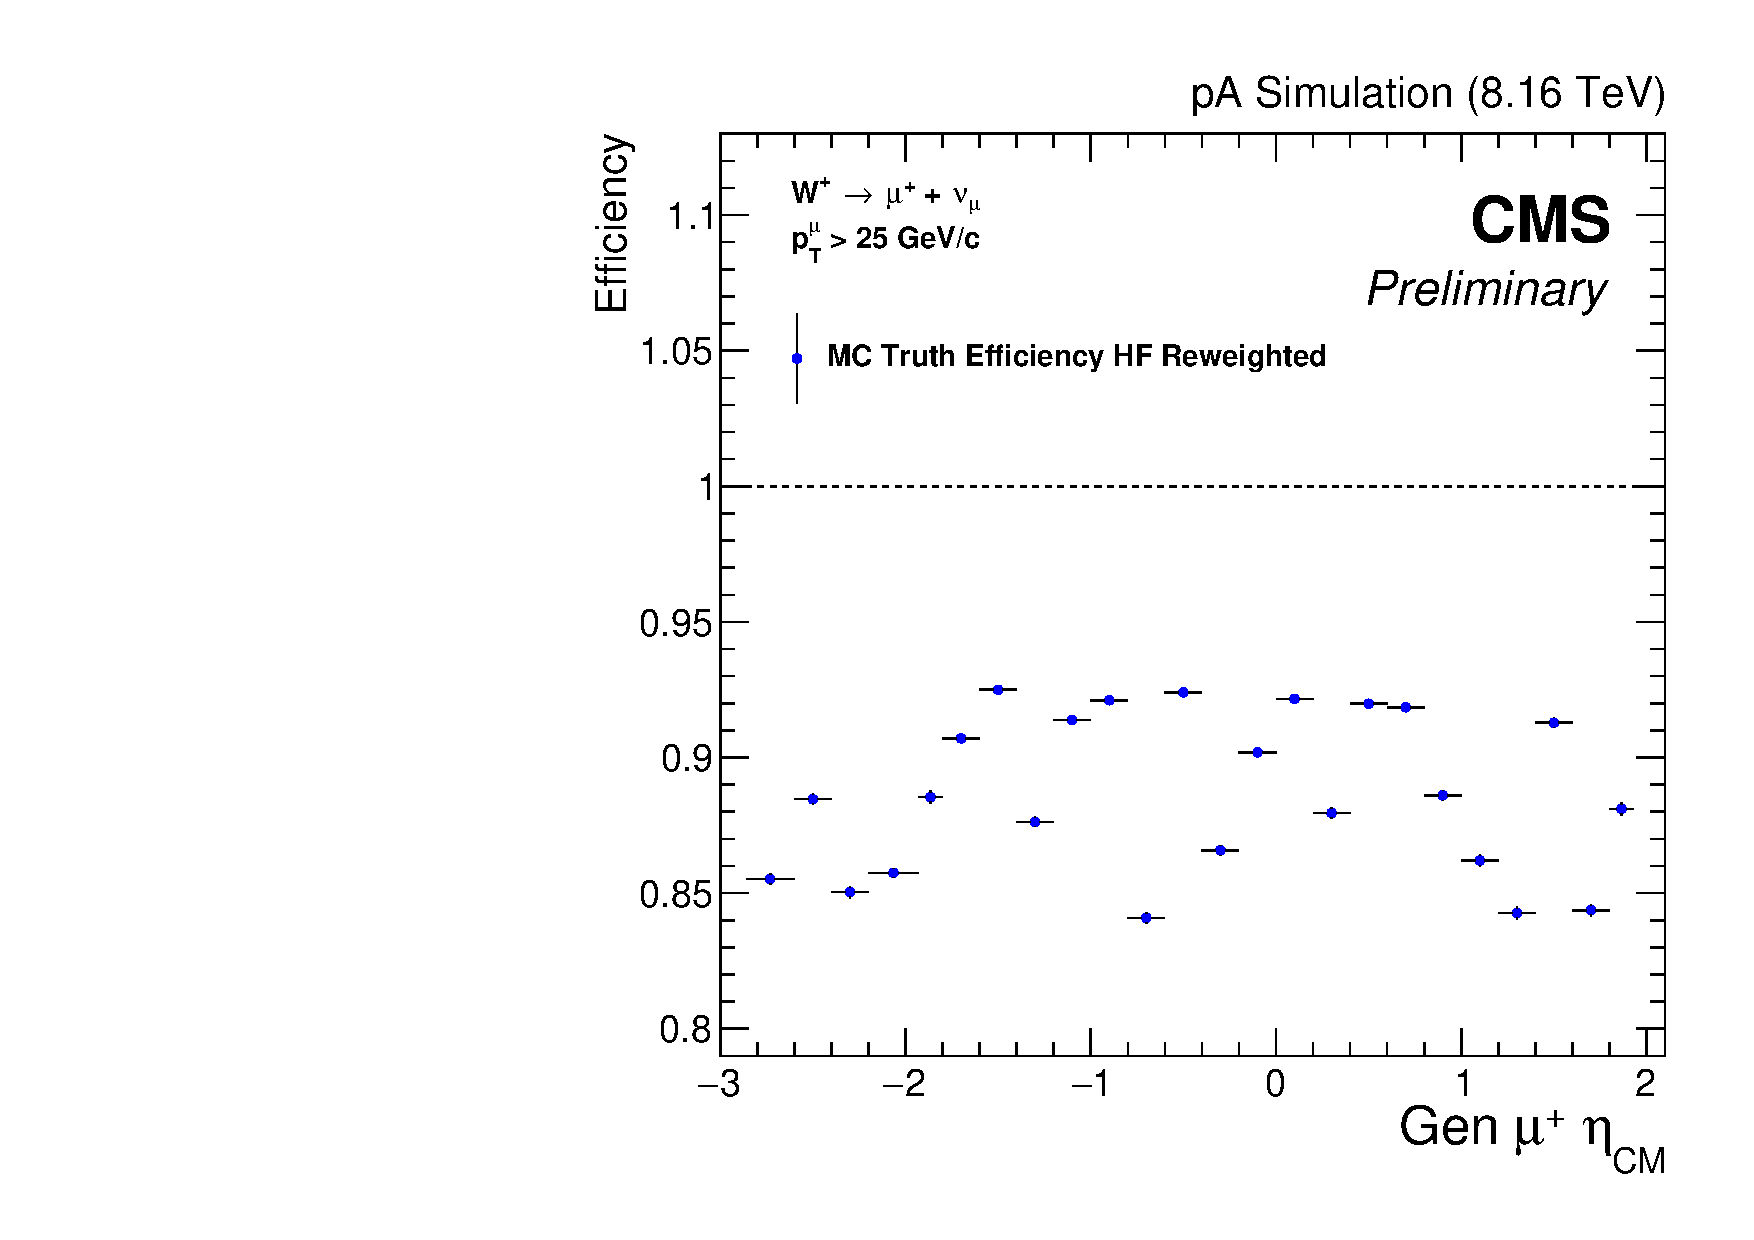
\includegraphics[width=0.45\textwidth]{Figures/WBoson/Analysis/Efficiency/Muon/PA/eff1D_EtaCM_MC_WToMuNu_PA_Plus_Total_HFCorrOnly}
 \end{center}
 \caption{Truth efficiency derived from \WToMuNu\ NLO MC sample as a function of the generated muon $\eta_{CM}$, separated in negative (left) and positive (right) charged muons. The event activity of the MC samples have been reweighed. Plots corresponds to \eq{eq:MCTruthEfficiency}, and the \RunpPb and \RunPbp MC efficiencies are combined according to \eq{eq:MCEfficiencyPA}. Only MC statistical errors are included.}
 \label{fig:MCTruthEfficiency}
\end{figure}

\subsection{Corrected muon efficiency}\label{sec:WBoson_Efficiency_CorrectedEfficiency}

The simulation of the CMS detector is very precise but still far from fully describing all the detector conditions observed in real data. In order to compensate for the imperfections in the simulations, the muon MC efficiency is corrected by applying a set of muon scale factors derived using the Tag-and-Probe method~\cite{Muon_TnP}.

The Tag-and-Probe (TnP) method is a data-driven technique widely used to compute efficiencies of physical objects, such as muons, produced from known mass resonances (e.g. \JPsi, \Z boson). One advantage of the TnP method is that it can be applied to both MC and real data, allowing to asses the differences between the data and MC efficiencies. For high \pt muons ($\pt > 15$~\GeVc), the \ZToMuMu decays are used to build a clean sample. In each event, one muon is classified as the "tag" if it has a $\pt > 15$~\GeVc and passes all the analysis cuts (trigger matching, isolation and identification), ensuring that it is a real muon, while the remaining muon is labelled as the "probe". Subsequently, the invariant mass distribution of the tag-probe dimuons is fitted in three cases: all pairs, failed pairs and passing pairs, depending on wether the probe muon passes or fails the selection criteria. The efficiency is calculated as a function of the probe \pt and $\eta_{LAB}$ in the laboratory frame by dividing the extracted yields of the passing pairs over all the pairs for various kinematic ranges of the probe. Finally, the TnP efficiencies in data and MC are compared, and the ratio of the two efficiencies is used to correct the simulations. More information about the \pPb TnP scale factors can be found in \cite{Muon_TnP_pPb}.

In this case, the muon efficiencies derived in \sect{sec:WBoson_Efficiency} are corrected by applying event by event the TnP scale factors as a function of muon $\eta_{LAB}$ and \pt. The statistical and systematic components of the TnP correction uncertainties are derived by applying the following set of variations:

\begin{enumerate}
   \item TnP statistical uncertainty:
   \begin{enumerate}
      \item For muon ID and isolation: 100 scale factor variations derived from toy MC.
      \item For trigger: Up and down $1 \sigma_{stat}$ variations.
   \end{enumerate}
   \item TnP systematic uncertainty:
   \begin{enumerate}
      \item For muon ID, isolation and trigger: Up and down by $1 \sigma_{syst}$ variations.
      \item For muon ID and isolation: Using the scale factor from the Data/MC bins instead of the one derived from fitting the ratio.
      \item For isolation: An uncertainty of {\bf 0.34\%} to account for the impact on the isolation efficiency of the different level of activity and pile-up between data and MC.
      \item For stand-alone muon reconstruction: An uncertainty of {\bf 0.6\%} to account for mismodelings in the STA efficiency.
   \end{enumerate}
\end{enumerate}

The uncertainties on the muon efficiency due to the TnP corrections are calculated in three different ways, as explained below.

\begin{enumerate}
   \item Taking the RMS between the 100 efficiencies corrected using the toy MC scale factors. Used in 1.a.
   \item Taking the maximum difference between the efficiency corrected using the nominal and the varied TnP scale factors. Used in 1.b, 2.a and 2.b.
   \item Applying the TnP scale factor uncertainty as a relative uncertainty on the corrected efficiency. Used in 2.c and 2.d.
\end{enumerate}

The total TnP uncertainty is obtained by summing in quadrature all the statistical and systematic TnP uncertainties. The TnP corrected efficiencies including their total uncertainties are shown in \fig{fig:CorrEfficiency}.

\begin{figure}[htb!]
 \begin{center}
  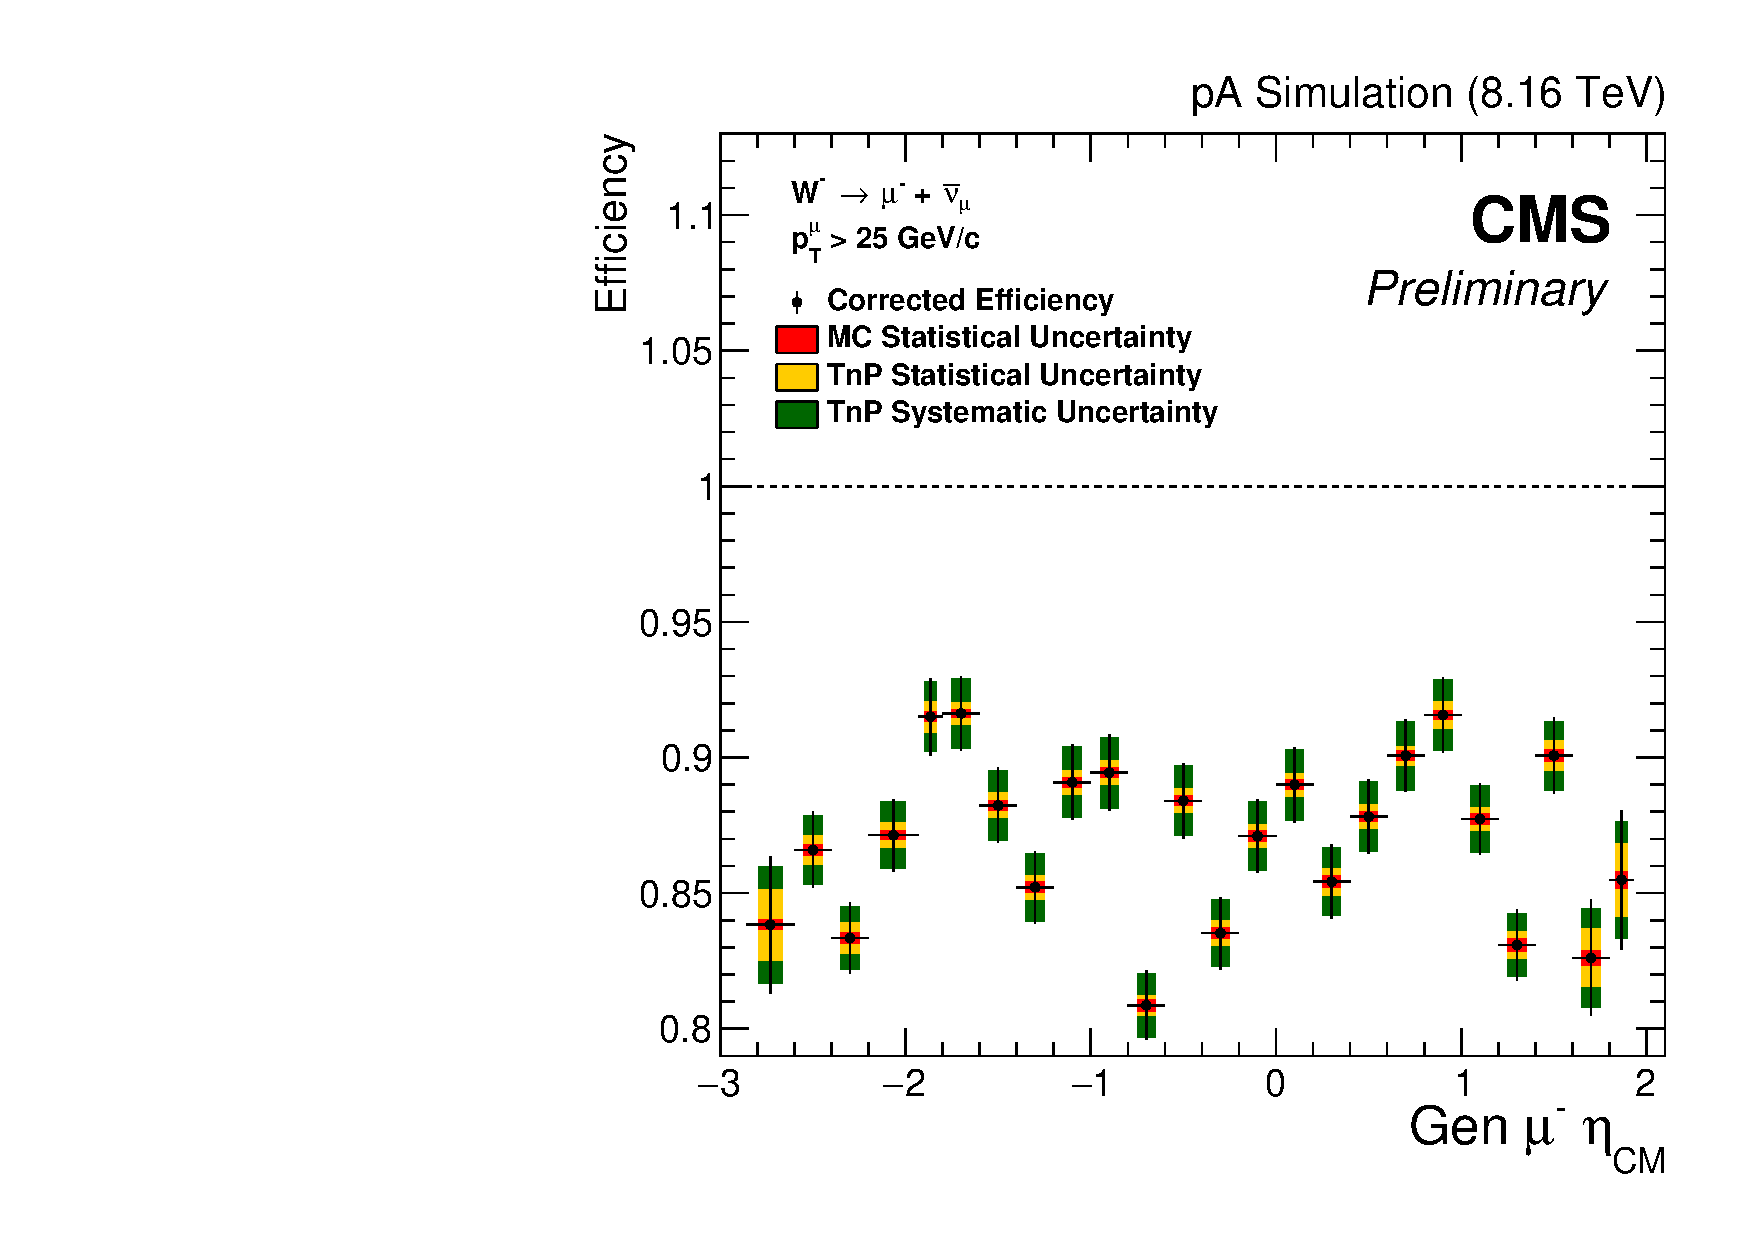
\includegraphics[width=0.45\textwidth]{Figures/WBoson/Analysis/Efficiency/Muon/PA/eff1D_EtaCM_MC_WToMuNu_PA_Minus_Total_TnP_Nominal}
  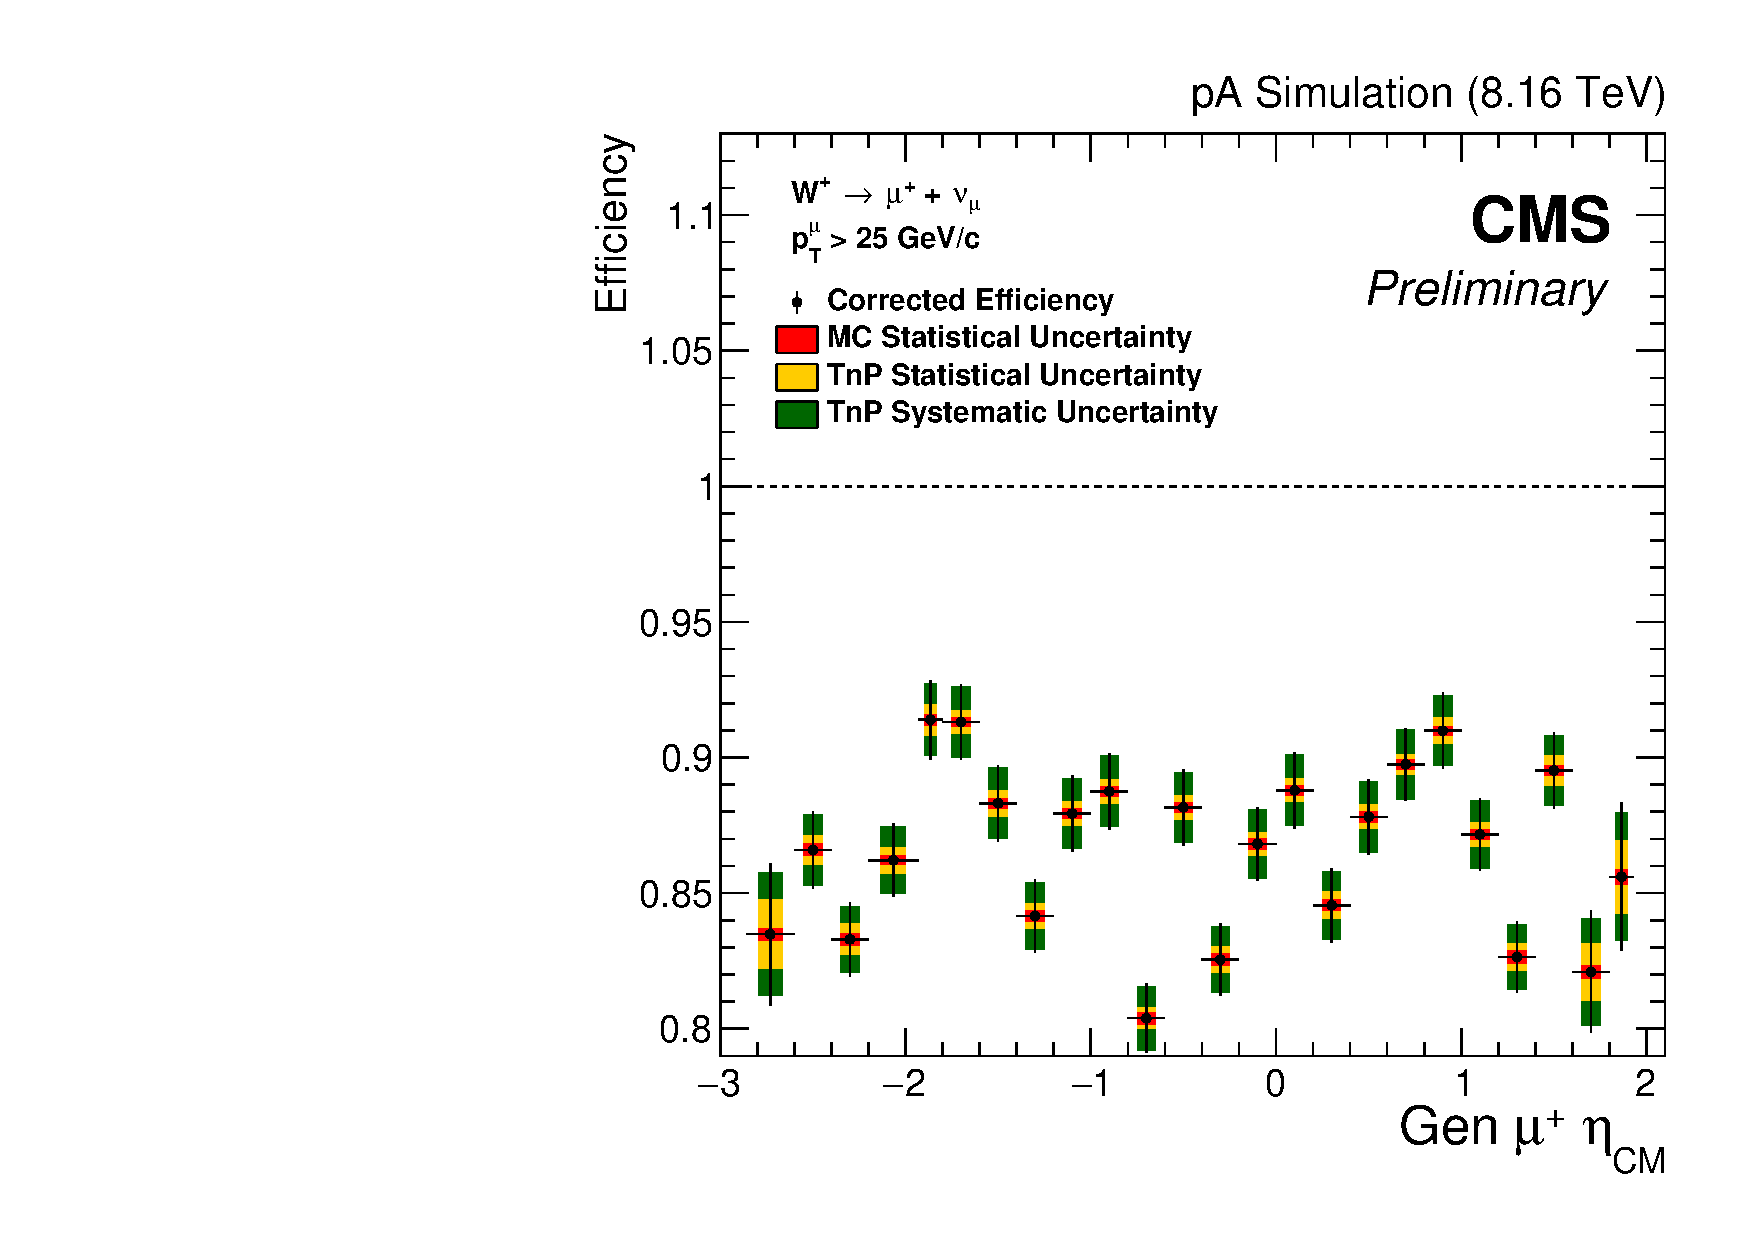
\includegraphics[width=0.45\textwidth]{Figures/WBoson/Analysis/Efficiency/Muon/PA/eff1D_EtaCM_MC_WToMuNu_PA_Plus_Total_TnP_Nominal}
 \end{center}
 \caption{Muon corrected efficiency derived from \WToMuNu \POWHEG MC sample as a function of the generated muon $\eta_{CM}$, separated in negative (left) and positive (right) charged muons. The muon efficiency has been corrected by applying the Tag and Probe scale factors event by event. The red, yellow and green boxes represents the uncertainty on the efficiency due to the MC statistics, TnP statistics and TnP systematics, respectively. The \RunpPb and \RunPbp MC efficiencies are combined according to \eq{eq:MCEfficiencyPA}.}
 \label{fig:CorrEfficiency}
\end{figure}


% END OF SUBSECTION



\section{Signal extraction}\label{sec:WBoson_SignalExtraction}

The signal and background yields are extracted by fitting the \ETslash\ \ distribution in data. The main background sources come from QCD and electroweak processes. The QCD background includes events where a high $p_{T}$ muon is produced from a semi-leptonic decay of quarks (multi-jet background). Most of these muons come from \PQb\ quark decays and light meson (pion and kaon) decays in flight. The dominant electroweak processes are the \DYToMuMu (Drell-Yan) and \WToTauNu as mentioned in \sect{sec:WBoson_SignalExtraction_EWKBackground}. The shape of the signal and background is estimated by using MET templates to describe the signal and the electroweak backgrounds, and a MET functional form derived from data to describe the multi-jet background as explained in \sect{sec:WBoson_SignalExtraction_QCDBackground}.

The simulated samples of \DYToMuMu , \DYToTauTau , \WToMuNu and \WToTauNu are normalized to the total integrated luminosity recorded in data using the NLO cross sections derived from the \POWHEG MC samples scaled by the number of nucleons in the Pb ion. The normalization is done by reweighing all MC events by a global factor defined as $w_{MC} = (\sigma\times\Lumi_{data})/N_{gen}$. In the case of the \ttbar MC, the samples are normalized using $\sigma_{\ttbar} = 45~\nbinv$, which corresponds to the total cross section measured in \pPb collisions at 8.16~\TeV recently published by CMS \cite{HIN-17-002}.

Several corrections are applied to the MC samples before producing the templates, in order to improve the description of the data. First, the event activity in the simulations is reweighed using the energy deposited in the HF calorimeters as explained in \sect{sec:WBoson_Corrections_EventActivityReweighing}. Afterwards, since the muon $\eta_{CM}$ distribution is used to bin the data, the MC muon efficiency is corrected by applying the nominal TnP scale factors event by event, as mentioned in \sect{sec:WBoson_Efficiency_CorrectedEfficiency}. And finally, the resolution of the hadronic recoil component of the MET in MC is corrected as shown in \sect{sec:WBoson_Corrections_RecoilCorrection}, improving the agreement of the MET distribution between data and MC. Once the signal and the EWK MC samples are fully corrected, the MC templates are extracted in each muon $\eta_{CM}$ bin, by creating a histogram of the MET distribution in bins of 2~\GeVc.


\subsection{QCD background}\label{sec:WBoson_SignalExtraction_QCDBackground}


The QCD background is described using a data-driven method. The functional form of the multi-jet \ETslash\ \ distribution is derived by fitting the MET in a region dominated by non-isolated muons selected after inverting the nominal muon isolation cut mentioned in \sect{sec:WBoson_Selection_MuonIdentification}. All analysis cuts are applied except for the muon isolation cut. The general strategy is to first determine the dependence of the QCD functional form with respect to the muon isolation and then extrapolate the QCD shape down to low muon isolation values (signal region).

The nominal QCD \ETslash\ \ functional form is based on a modified version of the Rayleigh distribution as shown in \eq{eq:QCD_Nominal}.

\begin{equation}
f_{QCD}\left(x\right) = x {e}^{-{{x}^{2}}/{\left(2\left(\sigma_{0} + \sigma_{1}\tilde{x} + \sigma_{2}\left(2{\tilde{x}}^{2}-1\right)\right)^{2}\right)}} \quad \textrm{, where} \quad \tilde{x} = (x/50) - 1
\label{eq:QCD_Nominal}
\end{equation}

The free parameters are $\sigma_{0}$ ,  $\sigma_{1}$ and $\sigma_{2}$. The fit parameters have been arranged following a Chebyshev polynomial of second order, to reduce the correlation between parameters and improve the stability of the fits.

In order to derive the muon isolation dependence of the QCD parameters, the \ETslash\ \ distribution function is fitted over the following five muon isolation bins : [ 0.4 , 0.5 , 0.6 , 0.7 , 0.8 , 0.9 ]. The normalization of the QCD background is left free in the fits to the data.

The bins with lower muon isolation values ($\text{iso} < 0.4$) are discarded due to the large contamination from EWK processes. The dependence of the three parameters $\sigma_{0}$ ,  $\sigma_{1}$ and $\sigma_{2}$ with the muon isolation variable is fitted by a linear function. The results of the linear fits are then used to  extrapolate the shape of the QCD background to the signal region (average muon isolation of 0.03), as shown in \fig{fig:QCD_Extrapolation}. The values of the parameters corresponding to this extrapolation are given in \tab{tab:QCD_Extrapolation}.

\begin{table}[htbp]
  \begin{center}
   \begin{tabular}{|c|c|c|}\hline
    Parameter & $QCD \to \mu^{-}$ & $QCD \to \mu^{+}$ \\\hline
    $\sigma_{0}$ & 14.59$\pm$0.18 & 14.72$\pm$0.17 \\\hline
    $\sigma_{1}$ & 6.30$\pm$0.24 & 6.76$\pm$0.23 \\\hline
    $\sigma_{2}$ & 0.49$\pm$0.15 & 0.47$\pm$0.13 \\\hline
   \end{tabular}
  \end{center}
  \caption{QCD shape parameters in the inclusive $\eta_{CM}$ bin, extrapolated to the signal region ($\text{iso} = 0.03$).}
  \label{tab:QCD_Extrapolation}
\end{table}

\begin{figure}[!htbp]
 \begin{center}
  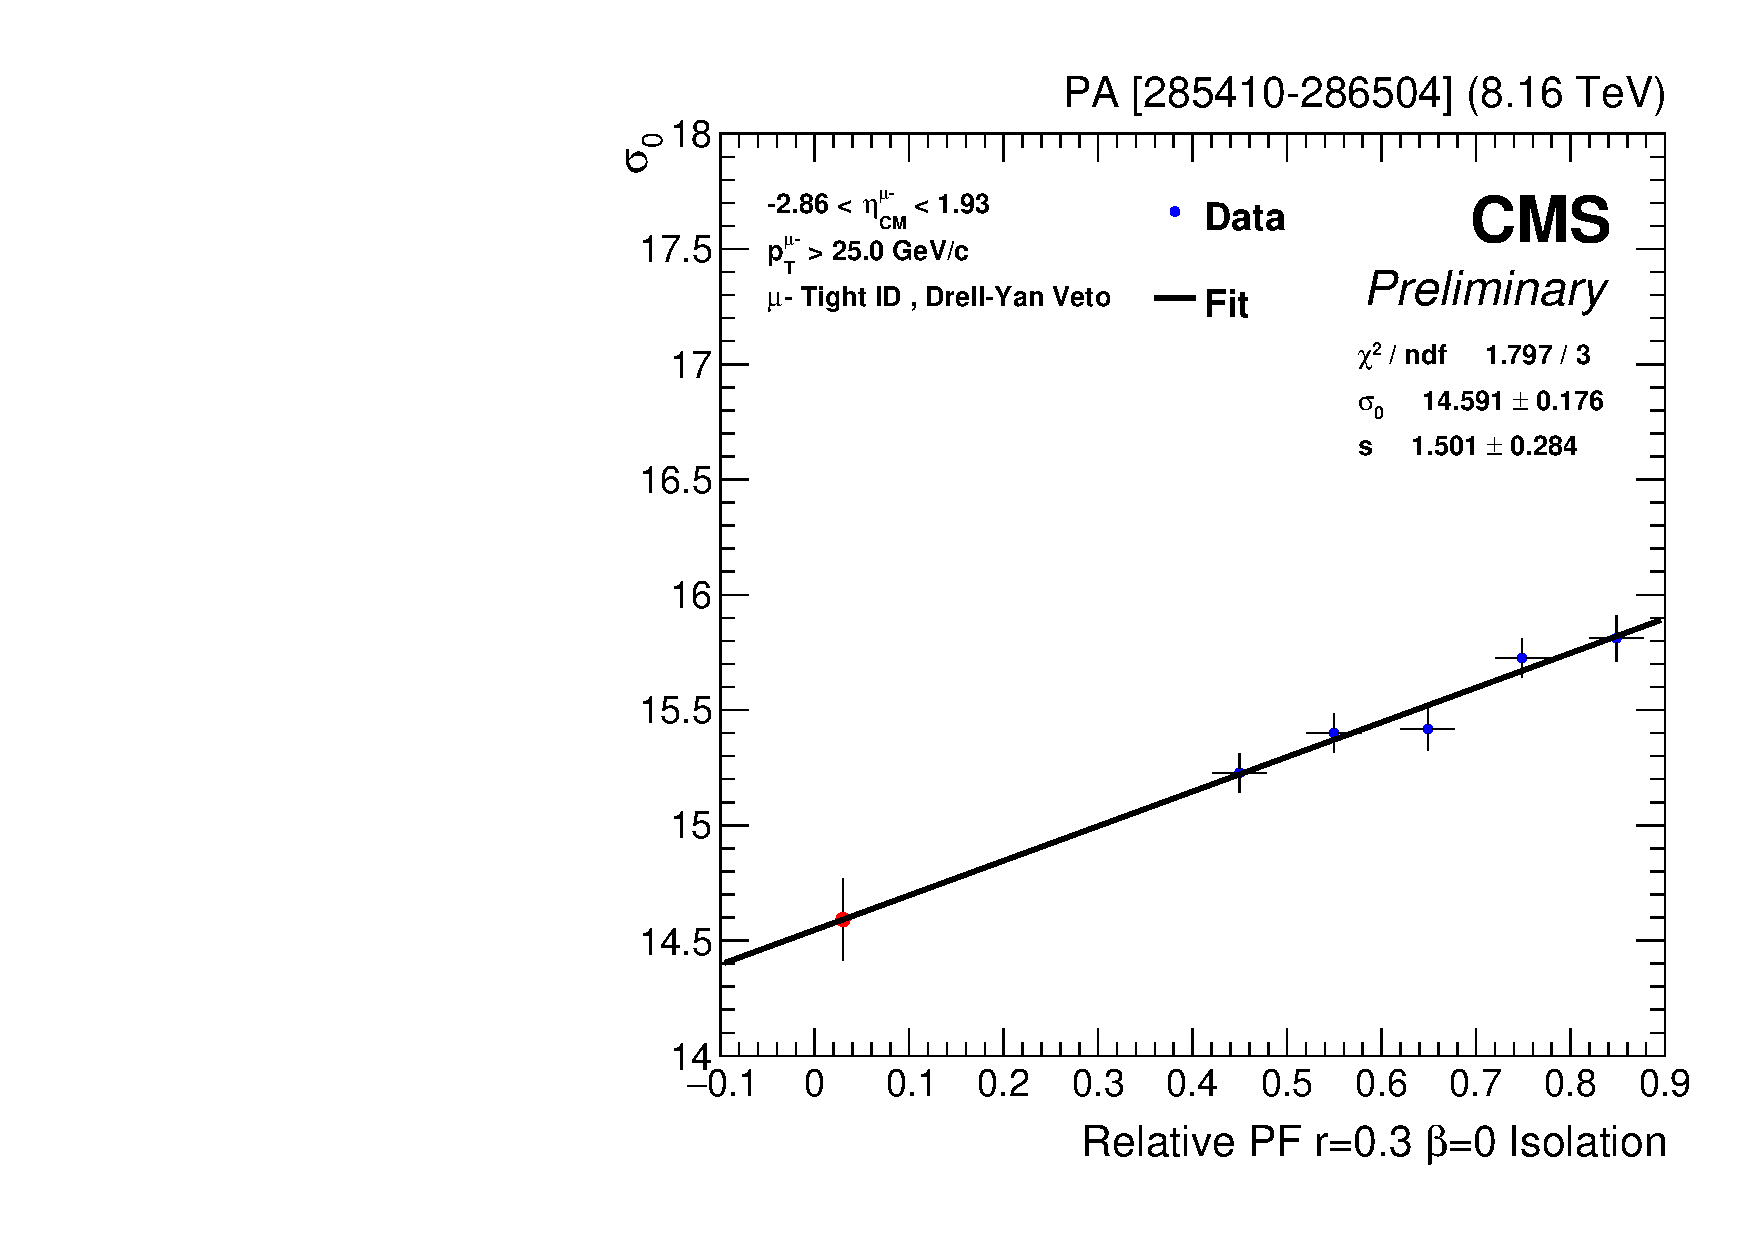
\includegraphics[width=0.27\textwidth]{Figures/WBoson/Analysis/SignalExtraction/QCD_Template/EXTRAPOLATION/PA/graph_Sigma0_QCDToMuMi_PA_-29_eta_19_250_pt_1000000.pdf}
  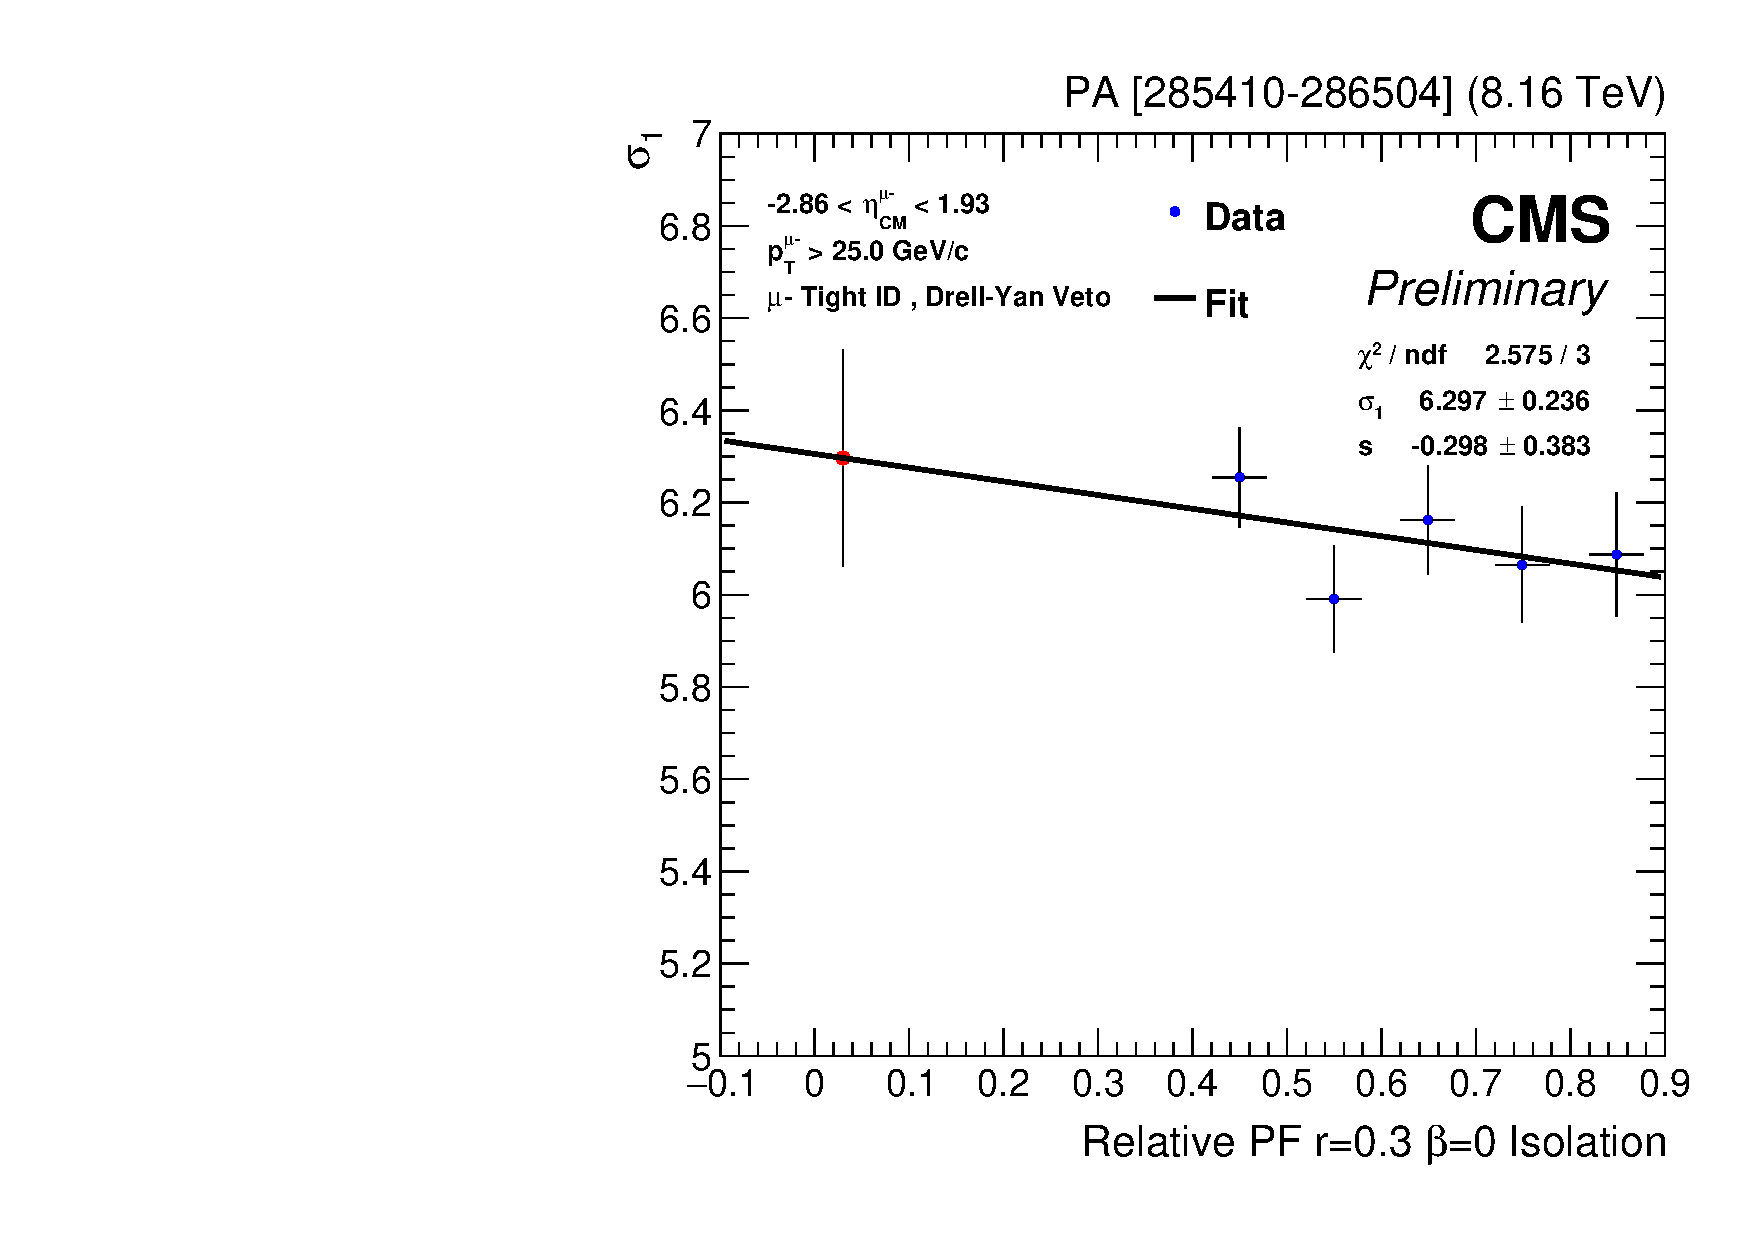
\includegraphics[width=0.27\textwidth]{Figures/WBoson/Analysis/SignalExtraction/QCD_Template/EXTRAPOLATION/PA/graph_Sigma1_QCDToMuMi_PA_-29_eta_19_250_pt_1000000.pdf}
  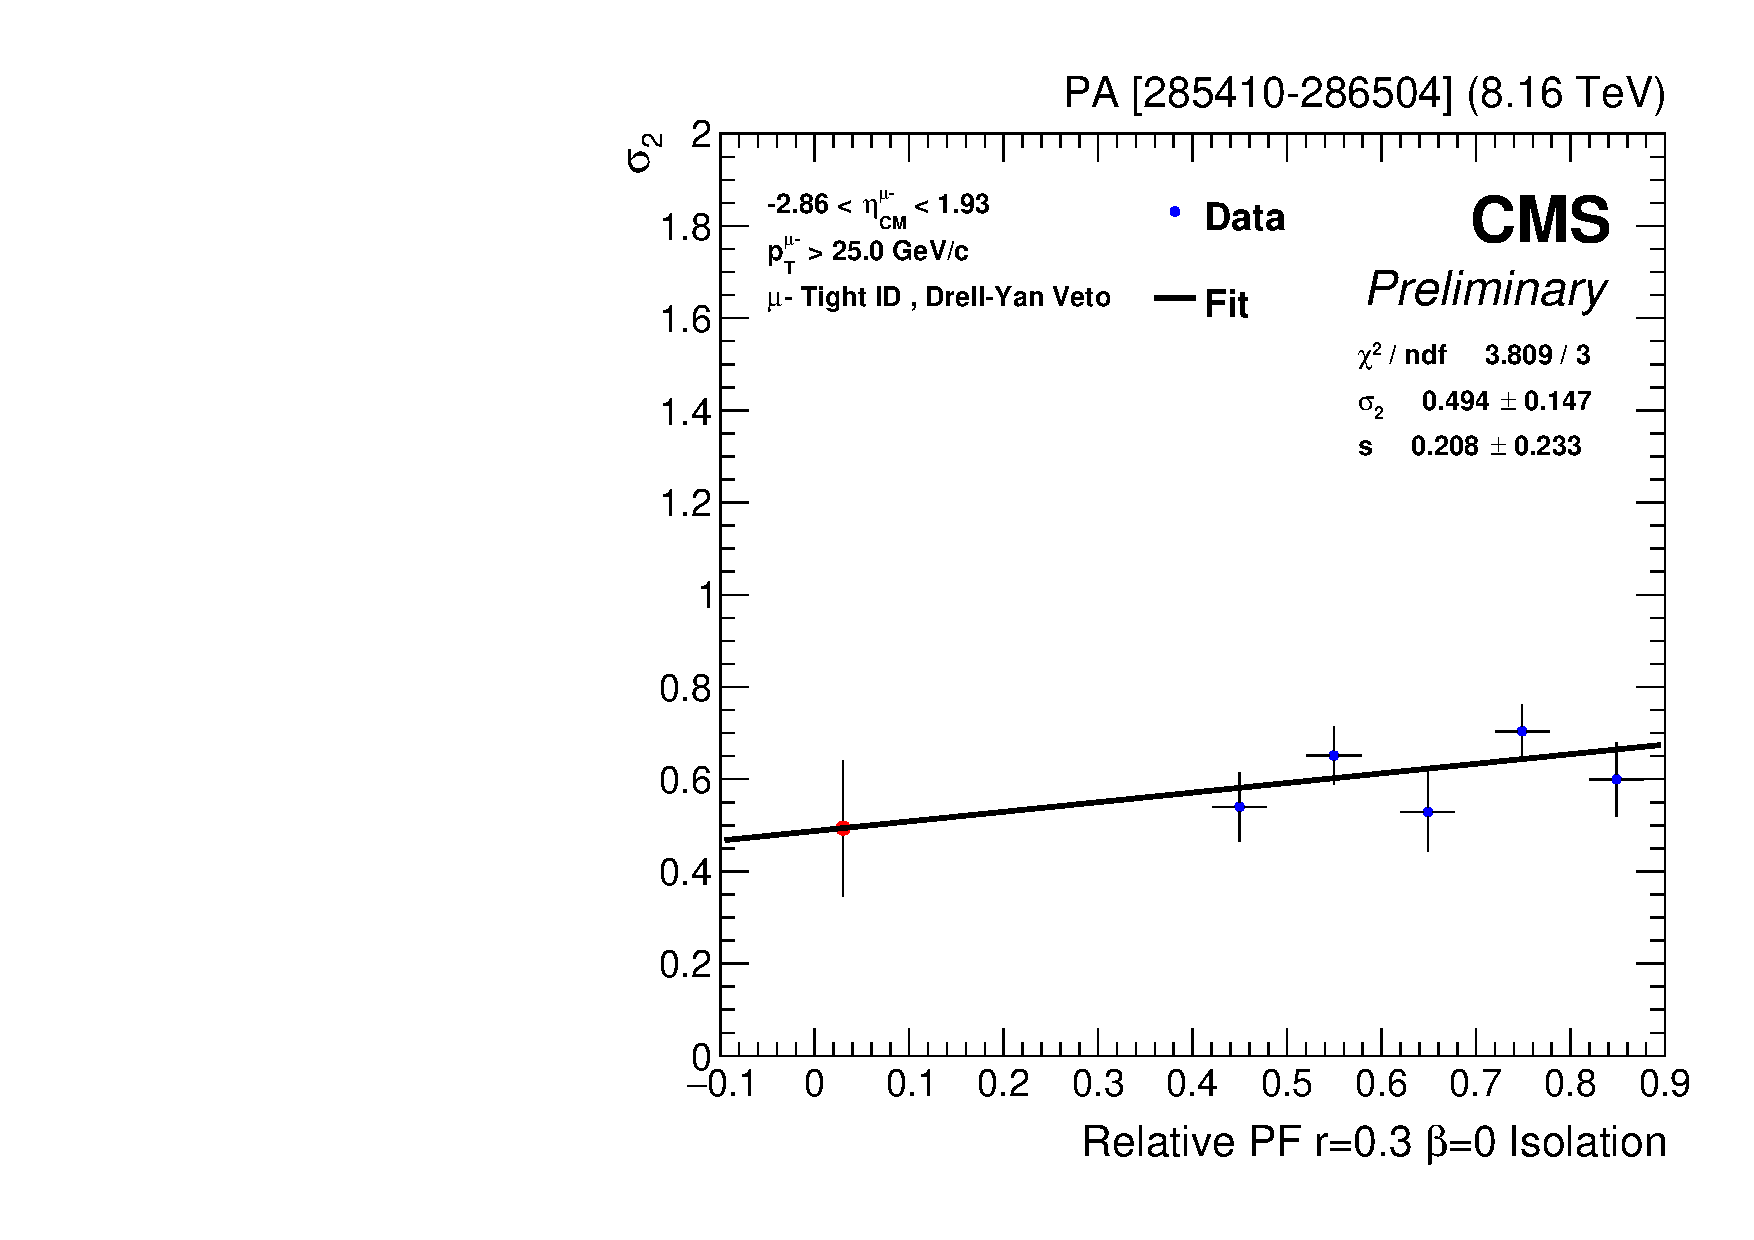
\includegraphics[width=0.27\textwidth]{Figures/WBoson/Analysis/SignalExtraction/QCD_Template/EXTRAPOLATION/PA/graph_Sigma2_QCDToMuMi_PA_-29_eta_19_250_pt_1000000.pdf}
%%
  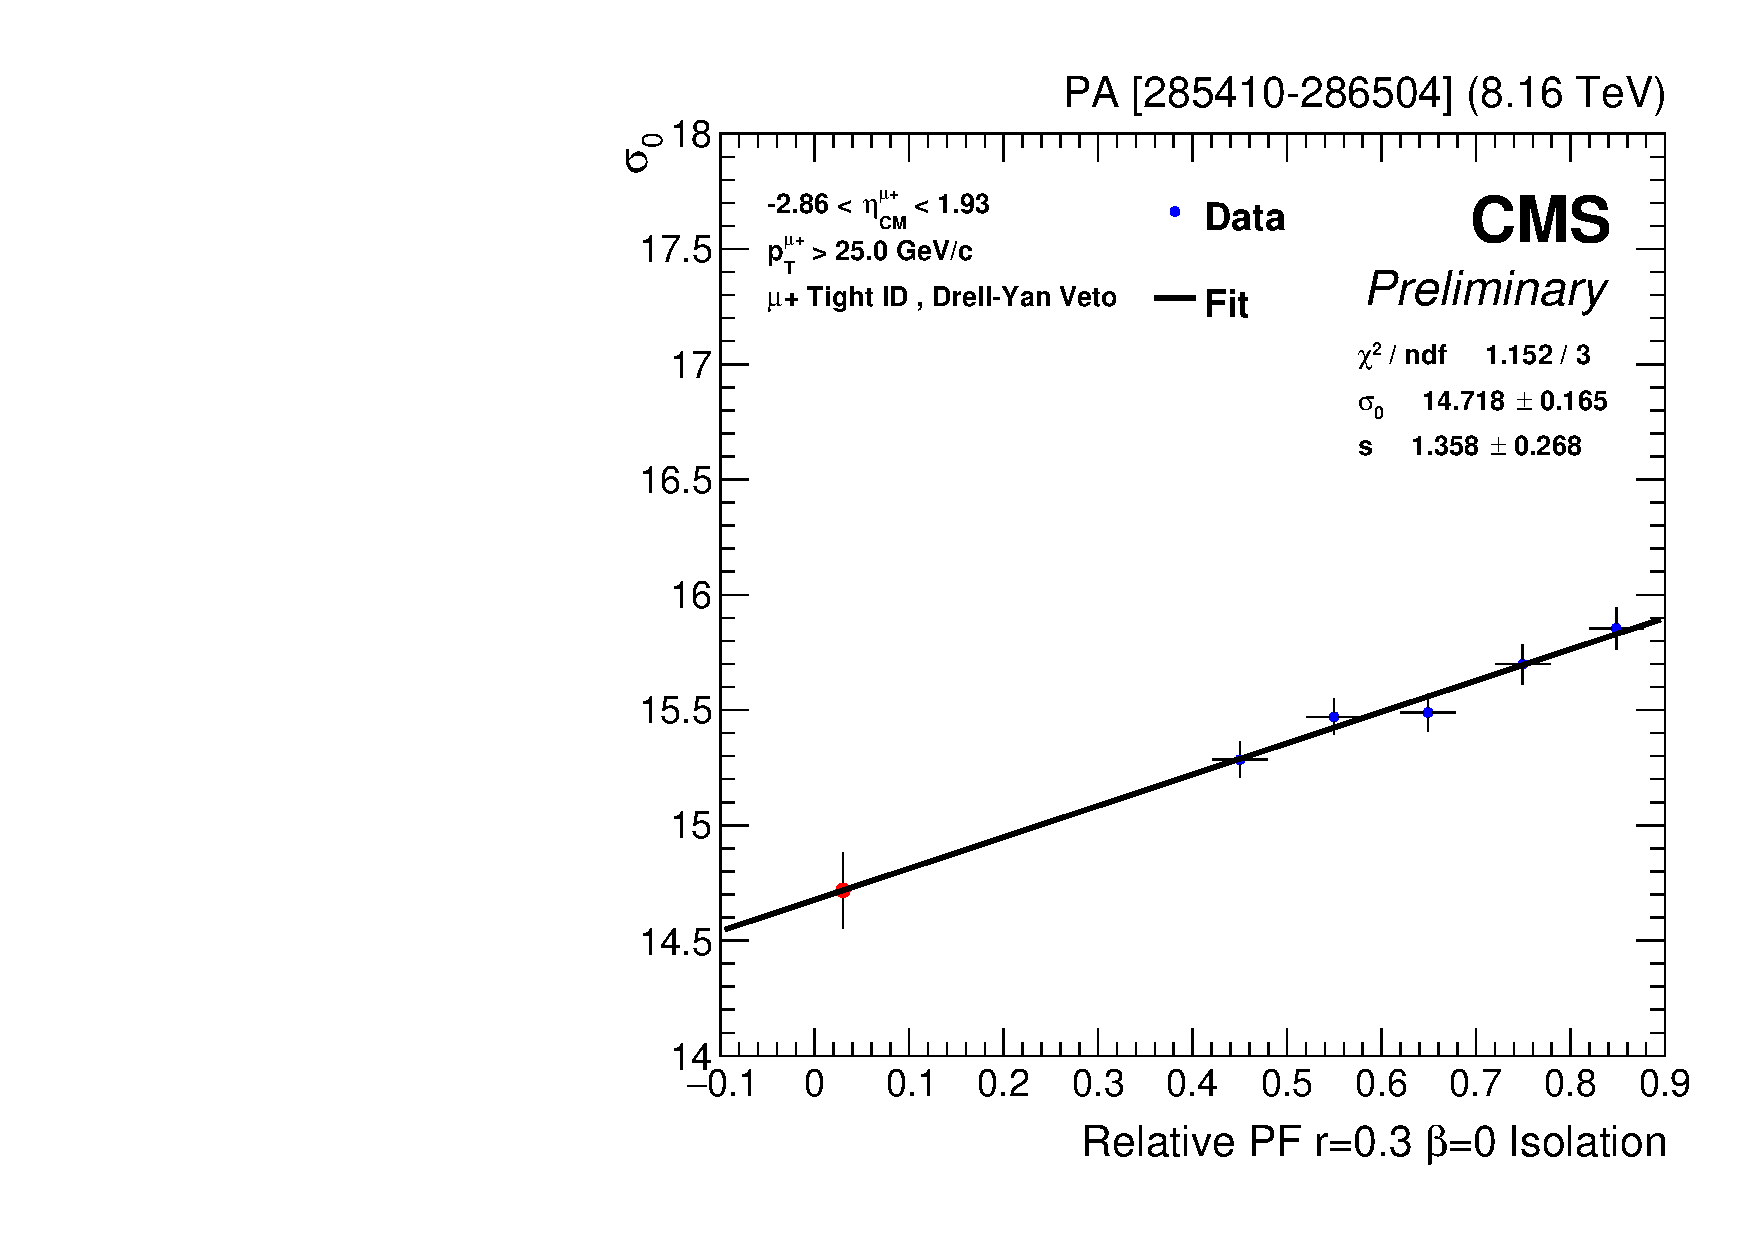
\includegraphics[width=0.27\textwidth]{Figures/WBoson/Analysis/SignalExtraction/QCD_Template/EXTRAPOLATION/PA/graph_Sigma0_QCDToMuPl_PA_-29_eta_19_250_pt_1000000.pdf}
  \includegraphics[width=0.27\textwidth]{Figures/WBoson/Analysis/SignalExtraction/QCD_Template/EXTRAPOLATION/PA/graph_Sigma1_QCDToMuPl_PA_-29_eta_19_250_pt_1000000.pdf}
  \includegraphics[width=0.27\textwidth]{Figures/WBoson/Analysis/SignalExtraction/QCD_Template/EXTRAPOLATION/PA/graph_Sigma2_QCDToMuPl_PA_-29_eta_19_250_pt_1000000.pdf}
 \end{center}
 \caption{Extrapolation of the parameters of the QCD background shape to the signal region: $\sigma_{0}$ (left), $\sigma_{1}$ (middle) and $\sigma_{2}$ (right), separated in negative (top) and positive (bottom) muon decays. Only the results inclusive in muon $\eta_{CM}$ are shown.}
 \label{fig:QCD_Extrapolation}
\end{figure}

The dependence on $\eta_{CM}$ of the QCD shape has been studied. The extrapolated results do not vary significantly with respect to $\eta_{CM}$ and have been found to be consistent with the $\eta$-inclusive results, within the fit uncertainties. Therefore, the $\eta$-inclusive extrapolated results for each muon charge are used to fix the QCD background shape when fitting the signal.


\subsection{Electroweak background}\label{sec:WBoson_SignalExtraction_EWKBackground}

Among all the electroweak background sources, the dominant one in the \W signal region is the Drell-Yan process. The Drell-Yan background is mainly made of \ZToMuMu events, where one of the muons is produced outside of the detector coverage ($|\eta|<$ 2.4) or did not pass the selection criteria. The other type of EWK sources considered in this analysis are \DYToTauTau, \WToTauNu and \ttbar. The EWK background represents around $13.3\%$ of the events in the signal region, divided as: \DYToMuMu ($9.4\%$), \WToTauNu ($2.4\%$), \DYToTauTau ($1.0\%$) and \ttbar ($0.5\%$). Other EWK processes such as double boson decays have been checked to contribute less than $0.03\%$, so they are not considered.

The contribution of each EWK background is described using \ETslash\ \ templates derived from the MC samples. The MET templates are produced following the procedure explained at the beginning of this section.


\subsection{Fit model}\label{sec:WBoson_SignalExtraction_FitModel}

The raw \WToMuNu yields are extracted by performing an unbinned log-likelihood fit of the observed \ETslash\ \ distribution in each muon $\eta_{CM}$ bin. The fits are done using a combination of binned templates and a continous functional form. The data analysis framework RooFit v3.60 \cite{RooFit} is used to make the fits.

The total fit model includes five contributions: the signal \WToMuNu template ($\mathcal{T}_{W}$), the EWK backgrounds \DYToMuMu, \WToTauNu, \DYToTauTau and \ttbar templates ($\mathcal{T}_{EWK}$), and the QCD data-driven functional form ($\mathcal{F}_{QCD}$). The model used to fit the data is shown in \eq{eq:FitModel}.

\begin{equation}
\resizebox{0.935\textwidth}{!}{%
${ N_{\W} \times \left( {\mathcal{T}_{\W}} + {r_{\DYToMuMu} \cdot \mathcal{T}_{\DYToMuMu}} + {r_{\WToTauNu} \cdot \mathcal{T}_{\WToTauNu}} + {r_{\DYToTauTau} \cdot \mathcal{T}_{\DYToTauTau}} + {r_{\ttbar} \cdot \mathcal{T}_{\ttbar}} \right) } + { N_{QCD} \times \mathcal{F}_{QCD} }$%
}
\label{eq:FitModel}
\end{equation}

The signal and the EWK background shapes are defined based on \ETslash\ \ templates, evaluated from MC simulations. Since the fits become too unstable if the EWK background yields are left free, the following criteria is used to constrain their yields. First, the \DYToMuMu , \WToTauNu, \DYToTauTau and the \ttbar raw yields are expressed in terms of $N_{EWK} = r_{EWK}\times N_{W}$. Afterwards, the ratio of raw yields ($r_{EWK}$) is fixed to its corresponding value derived from MC after having normalized all the MC samples to the recorded integrated luminosity and applied all analysis corrections and selection cuts. This criteria assume that the nuclear modification of the electroweak sources scales in the same way as the \W signal, which is expected at least for the \WToTauNu and the \DY processes.

The QCD contribution, as explained in section~\ref{sec:WBoson_SignalExtraction_QCDBackground}, is taken into account by means of a functional form depending on three parameters. For the fit of the \ETslash\ \  distribution the $\sigma_{0}$ , $\sigma_{1}$ and $\sigma_{2}$ are fixed to the extrapolated values mentioned in \tab{tab:QCD_Extrapolation}.

The \ETslash\ \ distribution is fitted separately for \WToMuNuPl and \WToMuNuMi candidates. Only the signal raw yield ($N_{\W}$) and the QCD normalization ($N_{QCD}$) are left free when fitting the \W signal region. The fits are done in both the inclusive selected events and in bins of muon pseudorapidity in the center of mass frame $\eta_{CM}$.


\subsection{Raw yields}\label{sec:WBoson_SignalExtraction_RawYields}


The results of the fits to the data in each of the different muon $\eta_{CM}$ bins are summarized in \tab{tab:RawYields_WToMuMi_PA} for $\W^{-}$ and in \tab{tab:RawYields_WToMuPl_PA} for $\W^{+}$.

\begin{table}[h!]
  \centering
  \resizebox{\textwidth}{!}{
  \renewcommand{\arraystretch}{1.5}
  \begin{tabular}{|c|*9c|}
    \hline
    $\eta_{CM}$ Range & Total & Fitted & Signal & \DYToMuMu & \WToTauNu & \DYToTauTau & \ttbar & QCD & p-value ($\chi^{2}$)\\
    \hline\hline
    -2.86 , -2.60 & 5210 & 5210 & $4056 \pm 66$ & $563 \pm 9$ & $137 \pm 2$ & $46 \pm 1$ & $3 \pm 0$ & $405 \pm 40$ & 0.42\\
    \hline
    -2.60 , -2.40 & 4308 & 4308 & $3407 \pm 60$ & $465 \pm 8$ & $104 \pm 2$ & $37 \pm 1$ & $4 \pm 0$ & $292 \pm 36$ & 0.31\\
    \hline
    -2.40 , -2.20 & 4273 & 4273 & $3290 \pm 60$ & $450 \pm 8$ & $103 \pm 2$ & $37 \pm 1$ & $5 \pm 0$ & $388 \pm 38$ & 0.26\\
    \hline
    -2.20 , -1.93 & 6423 & 6423 & $4936 \pm 74$ & $659 \pm 10$ & $158 \pm 2$ & $63 \pm 1$ & $12 \pm 0$ & $595 \pm 48$ & 0.53\\
    \hline
    -1.93 , -1.80 & 3140 & 3140 & $2430 \pm 52$ & $309 \pm 7$ & $80 \pm 2$ & $29 \pm 1$ & $8 \pm 0$ & $285 \pm 34$ & 0.51\\
    \hline
    -1.80 , -1.60 & 4822 & 4822 & $3682 \pm 64$ & $438 \pm 8$ & $119 \pm 2$ & $46 \pm 1$ & $19 \pm 0$ & $518 \pm 43$ & 0.46\\
    \hline
    -1.60 , -1.40 & 4727 & 4727 & $3644 \pm 64$ & $395 \pm 7$ & $119 \pm 2$ & $39 \pm 1$ & $18 \pm 0$ & $512 \pm 43$ & 0.85\\
    \hline
    -1.40 , -1.20 & 4521 & 4521 & $3600 \pm 64$ & $347 \pm 6$ & $111 \pm 2$ & $46 \pm 1$ & $21 \pm 0$ & $397 \pm 40$ & 0.03\\
    \hline
    -1.20 , -1.00 & 4626 & 4626 & $3672 \pm 65$ & $312 \pm 6$ & $120 \pm 2$ & $51 \pm 1$ & $23 \pm 0$ & $448 \pm 42$ & 0.57\\
    \hline
    -1.00 , -0.80 & 4722 & 4722 & $3769 \pm 66$ & $284 \pm 5$ & $121 \pm 2$ & $46 \pm 1$ & $31 \pm 1$ & $470 \pm 43$ & 0.87\\
    \hline
    -0.80 , -0.60 & 4198 & 4198 & $3434 \pm 63$ & $247 \pm 5$ & $105 \pm 2$ & $46 \pm 1$ & $29 \pm 1$ & $337 \pm 39$ & 0.82\\
    \hline
    -0.60 , -0.40 & 4648 & 4648 & $3743 \pm 66$ & $253 \pm 4$ & $122 \pm 2$ & $55 \pm 1$ & $37 \pm 1$ & $438 \pm 43$ & 0.09\\
    \hline
    -0.40 , -0.20 & 4344 & 4344 & $3484 \pm 64$ & $233 \pm 4$ & $112 \pm 2$ & $51 \pm 1$ & $34 \pm 1$ & $430 \pm 41$ & 0.16\\
    \hline
    -0.20 , +0.00 & 4474 & 4474 & $3522 \pm 65$ & $267 \pm 5$ & $114 \pm 2$ & $44 \pm 1$ & $37 \pm 1$ & $490 \pm 43$ & 0.01\\
    \hline
    +0.00 , +0.20 & 4643 & 4643 & $3661 \pm 65$ & $318 \pm 6$ & $116 \pm 2$ & $48 \pm 1$ & $39 \pm 1$ & $461 \pm 43$ & 0.00\\
    \hline
    +0.20 , +0.40 & 4638 & 4638 & $3538 \pm 64$ & $343 \pm 6$ & $112 \pm 2$ & $52 \pm 1$ & $43 \pm 1$ & $549 \pm 44$ & 0.00\\
    \hline
    +0.40 , +0.60 & 4718 & 4718 & $3538 \pm 63$ & $396 \pm 7$ & $117 \pm 2$ & $47 \pm 1$ & $38 \pm 1$ & $583 \pm 44$ & 0.30\\
    \hline
    +0.60 , +0.80 & 4552 & 4552 & $3382 \pm 62$ & $456 \pm 8$ & $106 \pm 2$ & $49 \pm 1$ & $34 \pm 1$ & $525 \pm 43$ & 0.64\\
    \hline
    +0.80 , +1.00 & 4637 & 4637 & $3331 \pm 61$ & $496 \pm 9$ & $106 \pm 2$ & $43 \pm 1$ & $39 \pm 1$ & $622 \pm 44$ & 0.00\\
    \hline
    +1.00 , +1.20 & 4612 & 4612 & $3281 \pm 60$ & $545 \pm 10$ & $108 \pm 2$ & $45 \pm 1$ & $27 \pm 0$ & $605 \pm 44$ & 0.54\\
    \hline
    +1.20 , +1.40 & 4053 & 4053 & $2761 \pm 54$ & $532 \pm 11$ & $78 \pm 2$ & $39 \pm 1$ & $22 \pm 0$ & $621 \pm 42$ & 0.11\\
    \hline
    +1.40 , +1.60 & 4251 & 4251 & $2924 \pm 56$ & $625 \pm 12$ & $100 \pm 2$ & $39 \pm 1$ & $21 \pm 0$ & $541 \pm 43$ & 0.16\\
    \hline
    +1.60 , +1.80 & 3844 & 3844 & $2511 \pm 51$ & $620 \pm 13$ & $79 \pm 2$ & $35 \pm 1$ & $15 \pm 0$ & $584 \pm 41$ & 0.06\\
    \hline
    +1.80 , +1.93 & 2640 & 2640 & $1724 \pm 42$ & $443 \pm 11$ & $55 \pm 1$ & $22 \pm 1$ & $9 \pm 0$ & $387 \pm 34$ & 0.44\\
    \hline
  \end{tabular}
  }
  \caption{Raw yields of \WToMuNuMi and background processes, extracted from the nominal fits for each muon $\eta_{CM}$ bin in the combined \pPb and \Pbp collision system. All analysis cuts are applied including the muon $p_{T} > 25$~GeV/c cut. All uncertainties shown are statistical only.}
  \label{tab:RawYields_WToMuMi_PA}
\end{table}


\begin{table}[h!]
  \centering
  \resizebox{\textwidth}{!}{
  \renewcommand{\arraystretch}{1.5}
  \begin{tabular}{|c|*9c|}
    \hline
    $\eta_{CM}$ Range & Total & Fitted & Signal & \DYToMuMu & \WToTauNu & \DYToTauTau & \ttbar & QCD & p-value ($\chi^{2}$)\\
    \hline\hline
    -2.86 , -2.60 & 4465 & 4465 & $3361 \pm 59$ & $589 \pm 10$ & $68 \pm 1$ & $46 \pm 1$ & $3 \pm 0$ & $397 \pm 38$ & 0.05\\
    \hline
    -2.60 , -2.40 & 4234 & 4234 & $3253 \pm 58$ & $533 \pm 10$ & $66 \pm 1$ & $37 \pm 1$ & $4 \pm 0$ & $341 \pm 36$ & 0.04\\
    \hline
    -2.40 , -2.20 & 4377 & 4377 & $3350 \pm 60$ & $503 \pm 9$ & $61 \pm 1$ & $37 \pm 1$ & $11 \pm 0$ & $415 \pm 38$ & 0.96\\
    \hline
    -2.20 , -1.93 & 6847 & 6846 & $5266 \pm 76$ & $723 \pm 10$ & $103 \pm 1$ & $55 \pm 1$ & $14 \pm 0$ & $686 \pm 49$ & 0.41\\
    \hline
    -1.93 , -1.80 & 3592 & 3591 & $2769 \pm 56$ & $340 \pm 7$ & $56 \pm 1$ & $30 \pm 1$ & $8 \pm 0$ & $388 \pm 36$ & 0.55\\
    \hline
    -1.80 , -1.60 & 5421 & 5417 & $4311 \pm 70$ & $496 \pm 8$ & $95 \pm 2$ & $51 \pm 1$ & $15 \pm 0$ & $449 \pm 44$ & 0.48\\
    \hline
    -1.60 , -1.40 & 5343 & 5343 & $4382 \pm 70$ & $451 \pm 7$ & $97 \pm 2$ & $46 \pm 1$ & $17 \pm 0$ & $350 \pm 42$ & 0.90\\
    \hline
    -1.40 , -1.20 & 5129 & 5125 & $4198 \pm 70$ & $386 \pm 6$ & $100 \pm 2$ & $42 \pm 1$ & $22 \pm 0$ & $377 \pm 43$ & 0.12\\
    \hline
    -1.20 , -1.00 & 5382 & 5380 & $4475 \pm 72$ & $344 \pm 6$ & $102 \pm 2$ & $56 \pm 1$ & $26 \pm 0$ & $378 \pm 43$ & 0.23\\
    \hline
    -1.00 , -0.80 & 5467 & 5464 & $4499 \pm 73$ & $314 \pm 5$ & $101 \pm 2$ & $51 \pm 1$ & $30 \pm 0$ & $469 \pm 45$ & 0.05\\
    \hline
    -0.80 , -0.60 & 4738 & 4737 & $3971 \pm 69$ & $251 \pm 4$ & $91 \pm 2$ & $43 \pm 1$ & $28 \pm 0$ & $352 \pm 41$ & 0.18\\
    \hline
    -0.60 , -0.40 & 5349 & 5349 & $4446 \pm 73$ & $263 \pm 4$ & $101 \pm 2$ & $49 \pm 1$ & $36 \pm 1$ & $454 \pm 45$ & 0.16\\
    \hline
    -0.40 , -0.20 & 5027 & 5023 & $4154 \pm 70$ & $246 \pm 4$ & $91 \pm 2$ & $47 \pm 1$ & $35 \pm 1$ & $450 \pm 44$ & 0.12\\
    \hline
    -0.20 , +0.00 & 5161 & 5160 & $4279 \pm 71$ & $276 \pm 5$ & $101 \pm 2$ & $47 \pm 1$ & $38 \pm 1$ & $419 \pm 43$ & 0.05\\
    \hline
    +0.00 , +0.20 & 5473 & 5471 & $4359 \pm 72$ & $315 \pm 5$ & $102 \pm 2$ & $55 \pm 1$ & $40 \pm 1$ & $600 \pm 47$ & 0.46\\
    \hline
    +0.20 , +0.40 & 5175 & 5175 & $4192 \pm 70$ & $343 \pm 6$ & $100 \pm 2$ & $49 \pm 1$ & $35 \pm 1$ & $457 \pm 44$ & 0.08\\
    \hline
    +0.40 , +0.60 & 5482 & 5481 & $4345 \pm 71$ & $409 \pm 7$ & $94 \pm 2$ & $44 \pm 1$ & $34 \pm 1$ & $555 \pm 47$ & 0.21\\
    \hline
    +0.60 , +0.80 & 5722 & 5719 & $4477 \pm 72$ & $482 \pm 8$ & $100 \pm 2$ & $51 \pm 1$ & $39 \pm 1$ & $569 \pm 47$ & 0.07\\
    \hline
    +0.80 , +1.00 & 6061 & 6061 & $4665 \pm 73$ & $570 \pm 9$ & $101 \pm 2$ & $48 \pm 1$ & $36 \pm 1$ & $641 \pm 48$ & 0.01\\
    \hline
    +1.00 , +1.20 & 5814 & 5814 & $4415 \pm 70$ & $609 \pm 10$ & $105 \pm 2$ & $41 \pm 1$ & $34 \pm 1$ & $610 \pm 47$ & 0.36\\
    \hline
    +1.20 , +1.40 & 5365 & 5362 & $4057 \pm 67$ & $574 \pm 9$ & $88 \pm 1$ & $35 \pm 1$ & $23 \pm 0$ & $585 \pm 45$ & 0.01\\
    \hline
    +1.40 , +1.60 & 5768 & 5768 & $4309 \pm 69$ & $680 \pm 11$ & $95 \pm 2$ & $41 \pm 1$ & $21 \pm 0$ & $622 \pm 47$ & 0.00\\
    \hline
    +1.60 , +1.80 & 5320 & 5320 & $3980 \pm 65$ & $667 \pm 11$ & $83 \pm 1$ & $34 \pm 1$ & $16 \pm 0$ & $541 \pm 44$ & 0.00\\
    \hline
    +1.80 , +1.93 & 3600 & 3599 & $2664 \pm 54$ & $456 \pm 9$ & $66 \pm 1$ & $20 \pm 0$ & $9 \pm 0$ & $384 \pm 37$ & 0.00\\
    \hline
  \end{tabular}
  }
  \caption{Raw yields of \WToMuNuPl and background processes, extracted from the nominal fits for each muon $\eta_{CM}$ bin in the combined \pPb and \Pbp collision system. All analysis cuts are applied including the muon $p_{T} > 25$~GeV/c cut. All uncertainties shown are statistical only.}
  \label{tab:RawYields_WToMuPl_PA}
\end{table}




\subsection{Corrected yields}\label{sec:WBoson_SignalExtraction_CorrectedYields}

The raw yields extracted from the fits are corrected taking into account the efficiency of the detector. The corrected yields are derived from the raw yields after dividing by the MC efficiency corrected with the Tag-And-Probe method as described in \sect{sec:WBoson_Efficiency_CorrectedEfficiency}. The formula used to derived the corrected yields is shown in \eq{eq:CorrectedYield}.

\begin{equation}
N^{\pm}_{corr} = \frac{N^{\pm}_{raw}}{\epsilon^{MC}_{corr}}
\label{eq:CorrectedYield}
\end{equation}

The statistical uncertainty of the corrected yields are computed based on error propagation according to the following equation:

\begin{equation}
\delta{N^{\pm}_{corr}} = \frac{\delta{N^{\pm}_{raw}}}{\epsilon^{MC}_{corr}}
\label{eq:CorrectedYieldStatError}
\end{equation}

The results of the corrected yields with respect to the muon $\eta_{CM}$ are summarized in \tab{tab:CorrYields_WToMuMi_PA} for $\W^{-}$ and in \tab{tab:CorrYields_WToMuPl_PA} for $\W^{+}$.

\begin{table}[!h]
  \centering
  \renewcommand{\arraystretch}{1.5}
  \begin{tabular}{|c|*3c|}
    \hline
    $\eta_{CM}$ Range & Raw Yield & Efficiency ($\%$) & Corrected Yield\\
    \hline\hline
    -2.86 , -2.60 & $4056 \pm 66$ & $83.83 \pm 0.21$ & $4839 \pm 78$\\
    \hline
    -2.60 , -2.40 & $3407 \pm 60$ & $86.60 \pm 0.22$ & $3935 \pm 70$\\
    \hline
    -2.40 , -2.20 & $3290 \pm 60$ & $83.34 \pm 0.23$ & $3947 \pm 72$\\
    \hline
    -2.20 , -1.93 & $4936 \pm 74$ & $87.14 \pm 0.17$ & $5664 \pm 85$\\
    \hline
    -1.93 , -1.80 & $2430 \pm 52$ & $91.51 \pm 0.20$ & $2655 \pm 57$\\
    \hline
    -1.80 , -1.60 & $3682 \pm 64$ & $91.63 \pm 0.15$ & $4018 \pm 70$\\
    \hline
    -1.60 , -1.40 & $3644 \pm 64$ & $88.23 \pm 0.23$ & $4130 \pm 73$\\
    \hline
    -1.40 , -1.20 & $3600 \pm 64$ & $85.22 \pm 0.22$ & $4224 \pm 75$\\
    \hline
    -1.20 , -1.00 & $3672 \pm 65$ & $89.09 \pm 0.20$ & $4122 \pm 73$\\
    \hline
    -1.00 , -0.80 & $3769 \pm 66$ & $89.45 \pm 0.21$ & $4214 \pm 74$\\
    \hline
    -0.80 , -0.60 & $3434 \pm 63$ & $80.87 \pm 0.24$ & $4246 \pm 78$\\
    \hline
    -0.60 , -0.40 & $3743 \pm 66$ & $88.40 \pm 0.22$ & $4234 \pm 75$\\
    \hline
    -0.40 , -0.20 & $3484 \pm 64$ & $83.53 \pm 0.24$ & $4171 \pm 77$\\
    \hline
    -0.20 , +0.00 & $3522 \pm 65$ & $87.10 \pm 0.23$ & $4043 \pm 74$\\
    \hline
    +0.00 , +0.20 & $3661 \pm 65$ & $89.00 \pm 0.22$ & $4114 \pm 73$\\
    \hline
    +0.20 , +0.40 & $3538 \pm 64$ & $85.43 \pm 0.24$ & $4141 \pm 75$\\
    \hline
    +0.40 , +0.60 & $3538 \pm 63$ & $87.82 \pm 0.23$ & $4028 \pm 72$\\
    \hline
    +0.60 , +0.80 & $3382 \pm 62$ & $90.07 \pm 0.21$ & $3755 \pm 68$\\
    \hline
    +0.80 , +1.00 & $3331 \pm 61$ & $91.57 \pm 0.17$ & $3638 \pm 66$\\
    \hline
    +1.00 , +1.20 & $3281 \pm 60$ & $87.73 \pm 0.21$ & $3740 \pm 68$\\
    \hline
    +1.20 , +1.40 & $2761 \pm 54$ & $83.09 \pm 0.24$ & $3323 \pm 66$\\
    \hline
    +1.40 , +1.60 & $2924 \pm 56$ & $90.07 \pm 0.23$ & $3246 \pm 62$\\
    \hline
    +1.60 , +1.80 & $2511 \pm 51$ & $82.61 \pm 0.28$ & $3040 \pm 62$\\
    \hline
    +1.80 , +1.93 & $1724 \pm 42$ & $85.49 \pm 0.33$ & $2016 \pm 49$\\
    \hline
  \end{tabular}
  \caption{Corrected yields of \WToMuNuMi, given for each muon $\eta_{CM}$ bin in the combined \pPb and \Pbp collision system. All analysis cuts are applied including the muon $p_{T} > 25$~GeV/c cut. The muon efficiency has been corrected by applying the Tag and Probe scale factors event by event. All uncertainties shown are statistical only.}
  \label{tab:CorrYields_WToMuMi_PA}
\end{table}


\begin{table}[!h]
  \centering
  \renewcommand{\arraystretch}{1.5}
  \begin{tabular}{|c|*3c|}
    \hline
    $\eta_{CM}$ Range & Raw Yield & Efficiency ($\%$) & Corrected Yield\\
    \hline\hline
    -2.86 , -2.60 & $3361 \pm 59$ & $83.49 \pm 0.24$ & $4026 \pm 71$\\
    \hline
    -2.60 , -2.40 & $3253 \pm 58$ & $86.60 \pm 0.24$ & $3757 \pm 67$\\
    \hline
    -2.40 , -2.20 & $3350 \pm 60$ & $83.29 \pm 0.24$ & $4022 \pm 72$\\
    \hline
    -2.20 , -1.93 & $5266 \pm 76$ & $86.21 \pm 0.18$ & $6108 \pm 88$\\
    \hline
    -1.93 , -1.80 & $2769 \pm 56$ & $91.40 \pm 0.18$ & $3030 \pm 61$\\
    \hline
    -1.80 , -1.60 & $4311 \pm 70$ & $91.31 \pm 0.16$ & $4721 \pm 76$\\
    \hline
    -1.60 , -1.40 & $4382 \pm 70$ & $88.31 \pm 0.21$ & $4962 \pm 79$\\
    \hline
    -1.40 , -1.20 & $4198 \pm 70$ & $84.15 \pm 0.24$ & $4988 \pm 83$\\
    \hline
    -1.20 , -1.00 & $4475 \pm 72$ & $87.94 \pm 0.23$ & $5089 \pm 82$\\
    \hline
    -1.00 , -0.80 & $4499 \pm 73$ & $88.75 \pm 0.23$ & $5069 \pm 82$\\
    \hline
    -0.80 , -0.60 & $3971 \pm 69$ & $80.39 \pm 0.24$ & $4940 \pm 85$\\
    \hline
    -0.60 , -0.40 & $4446 \pm 73$ & $88.16 \pm 0.22$ & $5043 \pm 83$\\
    \hline
    -0.40 , -0.20 & $4154 \pm 70$ & $82.55 \pm 0.24$ & $5032 \pm 85$\\
    \hline
    -0.20 , +0.00 & $4279 \pm 71$ & $86.81 \pm 0.22$ & $4929 \pm 82$\\
    \hline
    +0.00 , +0.20 & $4359 \pm 72$ & $88.79 \pm 0.21$ & $4910 \pm 81$\\
    \hline
    +0.20 , +0.40 & $4192 \pm 70$ & $84.55 \pm 0.24$ & $4958 \pm 82$\\
    \hline
    +0.40 , +0.60 & $4345 \pm 71$ & $87.81 \pm 0.22$ & $4948 \pm 81$\\
    \hline
    +0.60 , +0.80 & $4477 \pm 72$ & $89.75 \pm 0.21$ & $4989 \pm 80$\\
    \hline
    +0.80 , +1.00 & $4665 \pm 73$ & $90.99 \pm 0.16$ & $5127 \pm 80$\\
    \hline
    +1.00 , +1.20 & $4415 \pm 70$ & $87.16 \pm 0.23$ & $5065 \pm 80$\\
    \hline
    +1.20 , +1.40 & $4057 \pm 67$ & $82.64 \pm 0.24$ & $4909 \pm 81$\\
    \hline
    +1.40 , +1.60 & $4309 \pm 69$ & $89.52 \pm 0.20$ & $4813 \pm 77$\\
    \hline
    +1.60 , +1.80 & $3980 \pm 65$ & $82.10 \pm 0.25$ & $4848 \pm 79$\\
    \hline
    +1.80 , +1.93 & $2664 \pm 54$ & $85.60 \pm 0.29$ & $3112 \pm 63$\\
    \hline
  \end{tabular}
  \caption{Corrected yields of \WToMuNuPl, given for each muon $\eta_{CM}$ bin in the combined \pPb and \Pbp collision system. All analysis cuts are applied including the muon $p_{T} > 25$~GeV/c cut. The muon efficiency has been corrected by applying the Tag and Probe scale factors event by event. All uncertainties shown are statistical only.}
  \label{tab:CorrYields_WToMuPl_PA}
\end{table}




\clearpage


% END OF SUBSECTION


\subsection{Systematic uncertainties}\label{sec:WBoson_Analysis_Systematics}

This section presents the different sources and the procedure employed to determine the systematic uncertainties in the measurement of the \Wb-boson production in \RunpPb collisions. 

%%------------------------------------------------------------%%
\subsubsection{Luminosity}

The recorded integrated luminosity of the 2016 \RunpPb data sample is 173.4~\nbinv, and is known with a precision of 3.5\%~\cite{LUM-17-002}. Since the integrated luminosity cancels in forward-backward ratios and in the muon charge asymmetry, it only affects the measurement of the \WToMuNu differential cross sections. In this case, this 3.5\% systematic uncertainty is global and the bin-to-bin correlations is 100\%. This uncertainty is the dominant one on the \WToMuNu differential cross sections.


%%------------------------------------------------------------%%
\subsubsection{Signal efficiency}

The dominant systematic uncertainty on the forward-backward ratios and muon charge asymmetry are due to the estimation of the signal efficiency. Since the signal efficiencies are computed from simulations and corrected using the TnP corrections, two sources of systematic uncertainties are considered. The first one corresponds to the theoretical modelling of the simulated signal, which takes into account the uncertainty on the nuclear PDFs and the impact of the renormalisation and factorisation scales. The second source corresponds to the TnP correction uncertainties, which derives from the \ZToMuMu control sample used to extract the TnP data efficiencies.

\paragraph{Theoretical modelling.} The NLO model used to generate the simulations can impact the measurement of the signal efficiencies. The main sources of theoretical uncertainties include the choice of the nuclear parton distribution function (EPPS16+CT14), and the renormalisation and factorisation scales.

Since the PDFs are not calculable from first principles but are determined experimentally, in particular by the measurements reported here, the inclusion of any PDF introduces an additional systematic uncertainty. Thus, it is important to determine the impact of a change of PDF on the signal efficiencies. The procedure to derive the theoretical uncertainties of the PDF variations consist of reweighing the simulations event-by-event using weights derived from \POWHEG after applying various PDF sets. The PDF sets are accessed through the LHAPDF6~\cite{LHAPDF6} framework and consist of 56 CT14 PDFs and 40 EPPS16 nuclear corrections. Once the simulations are reweighed with each PDF set, the efficiencies are recomputed and used to recalculate all the observables. The nPDF uncertainty is determined by combining the EPPS16+CT14 PDF variations of the observables using the Hessian approach, as recommended by the EPPS16 authors~\cite{EPPS16}. 

Moreover, the uncertainty due to the renormalisation ($\mu_{R}$) and factorisation ($\mu_{F}$) scales is computed by varying these two scales in \POWHEG using the following six combinations:
\begin{equation*}
(\mu_{R} , \mu_{F}) = [\ (0.5 , 0.5)\ ,\ (1.0 , 0.5)\ ,\ (0.5 , 1.0)\ ,\ (1.0 , 2.0)\ ,\ (2.0 , 1.0)\ ,\ (2.0 , 2.0)\ ]
\end{equation*}

The simulations are reweighed event by event using the \POWHEG weights produced with each set of scales, then the efficiencies are recomputed and the observables are recalculated for each varied efficiency. The variations on the observables are combined by taking the envelope (i.e. the maximum variation in each \etaMuCM range).

The systematic uncertainties from the PDF and scale variations are summed in quadrature, and amount to 0.1\%. Thus, the theoretical uncertainties have negligible impact on the signal efficiencies.

\paragraph{Tag-and-probe correction.} The main source of systematic uncertainty in the measurement of the signal efficiency arises from the application of the TnP corrections. As mentioned in \sect{sec:WBoson_Analysis_Efficiency_Corrected}, the statistical and systematic uncertainties of the TnP corrections are derived from the muon identification, isolation and trigger efficiencies measured in data.

It is crucial to consider the correlation between the different TnP uncertainties as a function of muon pseudorapidity and its charge, since they could cancel in the forward-backward ratios and muon charge asymmetry. The statistical TnP variations are uncorrelated between the different \etaLAB ranges in which they were derived. The systematic TnP variations are considered to be fully correlated as a function of muon charge since the detector response is the same for muons and anti-muons, and uncorrelated between the different \etaCM ranges (spanning different detectors).

To compute the uncertainties, the muon charge asymmetry and the forward-backward ratios are recalculated for each efficiency derived by varying the TnP corrections. The TnP uncertainties are then determined by taking the difference between the value obtained with the varied TnP correction and its nominal value, combining the uncertainties as explained in \sect{sec:WBoson_Analysis_Efficiency_Corrected}. If the source of TnP correction is correlated in muon charge or pseudorapidity, the corresponding signal yields are varied at the same time. Moreover, for the \Wpm differential cross sections, the statistical and systematic TnP uncertainties are calculated by propagating the uncertainties on the corrected signal efficiency.

The systematic uncertainty due to the TnP corrections amounts to 3.2\% and the dominant TnP uncertainties  are derived from the TnP systematic variations of the muon isolation (2.5\%) and trigger (1.1\%) components.

%%------------------------------------------------------------%%
\subsubsection{QCD jet background}

The systematic uncertainty in the QCD jet background originates from the uncertainty in the modelling of the QCD jet \ptmiss distribution in the signal region. The nominal procedure consists in fixing the parameters of the modified Rayleigh distribution from the fits extrapolated from data as explained in \sect{sec:WBoson_Analysis_SignalExtraction_QCDBackground}. In order to estimate the uncertainty of the mismodelling of the QCD jet background shape, both the parameters and the functional form are varied.

\paragraph{QCD jet background parameters.} The first source of systematic uncertainty reflects the possible mismodelling of the QCD jet background shape due to the \etaMuCM dependence of the QCD background parameters. In order to check this, the parameters of the nominal QCD jet model are set free but constrained to be near their nominal values by using a Gaussian penalty. The width of the penalty Gaussian function is fixed, for a given QCD background parameter, to the root mean square (RMS) of the set of extrapolated results along all \etaMuCM ranges, shown in \fig{fig:QCD_Extrapolation_Eta}. The RMS values used in the Gaussian penalty for the $\sigma_{0}$,  $\sigma_{1}$ and  $\sigma_{2}$ parameters are presented in \tab{tab:QCDContrainPar}. The difference between the number of signal events extracted from the Gaussian-constrained fits and the nominal fits is taken as the systematic uncertainty, which is then propagated to all observables. This source of uncertainty is considered to be fully uncorrelated since the \ptmiss distribution in each \etaMuCM range is fitted separately.

\begin{table}[htb!]
  \centering
  \begin{tabular}{|c|c c|}\hline
  \multirow{2}{*}{Parameter} & \multicolumn{2}{|c|}{RMS} \\
   & $QCD \to \mu^{-}$ & $QCD \to \mu^{+}$ \\\hline
  $\sigma_{0}$ & 1.0 & 0.5 \\\hline
  $\sigma_{1}$ & 0.9 & 0.9\\\hline
  $\sigma_{2}$ & 0.7 & 0.6\\\hline
  \end{tabular}
  \caption{The RMS of the set of QCD background parameters extrapolated along all \etaMuCM regions.}
  \label{tab:QCDContrainPar}
\end{table}

Another systematic variation consists of changing the muon isolation point used to extrapolate the QCD background parameters. In the nominal case, the isolation point of 0.03 is determined from the average muon isolation value in data within the signal region. As an alternative case, the muon isolation distribution is checked in a QCD \PYTHIA simulated sample satisfying the signal selection criteria, and the average isolation value is determined to be approximately 0.08. As a result, the QCD background parameters are recomputed by extrapolating them to an isolation point of $\iso=0.08$, and the fits are redone by fixing the QCD background parameters to the extrapolated values in the \etaMuCM-inclusive range as in the nominal case. The difference between the number of signal events extracted from the fits using the varied QCD background shape and the nominal results is taken as the systematic uncertainty. This uncertainty is propagated to all observables. The QCD background parameters extrapolated to $\iso=0.08$ are listed in \tab{tab:QCDFixedPar_Iso0p08}. Since the result in each \etaMuCM range varies independently, the uncertainty is considered to be fully uncorrelated.

\begin{table}[htb!]
  \centering
  \begin{tabular}{|c|c|c|}\hline
   Parameter & $QCD \to \mu^{-}$ & $QCD \to \mu^{+}$ \\\hline
   $\sigma_{0}$ & 14.67 & 14.79 \\\hline
   $\sigma_{1}$ & 6.28 & 6.71 \\\hline
   $\sigma_{2}$ & 0.50 & 0.49 \\\hline
  \end{tabular}
  \caption{QCD shape parameters extrapolated to the average muon isolation point $\text{iso} = 0.08$.}
  \label{tab:QCDFixedPar_Iso0p08}
\end{table}

The systematic uncertainty associated to the \etaMuCM dependence of the QCD background parameters amounts to 1.1\%, while the uncertainty corresponding to the change of extrapolation point represents 0.2\%.

\paragraph{QCD jet background functional form.} To assign a systematic uncertainty due to the assumed functional form for modelling the QCD jet background \ptmiss distribution, the shape of the QCD jet background is described using a different model. The alternative \ptmiss functional form employed, taken from Ref.\cite{HIN-13-007}, is given by: 

\begin{equation}\label{eq:QCDMultiJet}
  f_{\text{QCD}}\left(\ptmiss\right) = \left(\ptmiss+x_0\right)^{\alpha}\cdot\exp\left(\beta\cdot\sqrt{\ptmiss+x_0}\right)
\end{equation}

The extrapolation procedure explained in \sect{sec:WBoson_Analysis_SignalExtraction_QCDBackground} is redone using the alternative model. All the fits are remade using the alternative QCD background functional form fixed to the parameters extrapolated in the \etaMuCM-inclusive range. The difference between the number of signal events measured using the alternative QCD background model and the nominal results is taken as the systematic uncertainty due to mismodelling of the QCD jet background shape. This systematic uncertainty is propagated to all observables and amounts to 0.6\%. The bin-to-bin correlation is taken to be fully uncorrelated.

%%------------------------------------------------------------%%
\subsubsection{Electroweak and \ttbar backgrounds}

The \ttbar background and the different sources of electroweak background are described using template histograms derived from simulations. The simulated samples are scaled to the recorded integrated luminosity of data using the NLO \POWHEG cross sections for the electroweak processes and the CMS measured cross section for the \ttbar production. Since for each these background sources, the ratio of background over signal events is fixed to simulation when performing the fits, a systematic uncertainty is assigned to each source by varying up and down their cross sections as explained below. The systematic uncertainty in each \etaMuCM range is derived by taking the maximum difference between the nominal and the up/down variations. The bin-to-bin correlations in muon charge and pseudorapidity are considered correlated since the total cross section is used to normalise all simulated events.

\paragraph{\texorpdfstring{\DYToMuMu}\ background.} The uncertainty on the ratio of $\Z/\Wb$ total cross sections is estimated using the Monte Carlo for FeMtobarn processes (MCFM) program~\cite{MCFM} at NLO with the CT14+EPPS16 nuclear PDFs. A relative uncertainty of $0.8\%$ for $Z/\Wm$ and $1.3\%$ for $Z/\Wp$ cross-section ratios is determined with MCFM taking into account the PDF uncertainties. Since the cross sections in the muon channel depend on the branching ratio associated to each process, their uncertainty has to also be taken into account. The values of the branching ratios correspond to $\textrm{BR}(\ZToMuMu) = (3.366 \pm 0.007)\%$ and $\textrm{BR}(\WToMuNu) = (10.63 \pm 0.15)\%$~\cite{PDG}, which gives a relative uncertainty on the ratio of $\Z/\Wb$ branching ratios of $1.4\%$. Summing in quadrature the MCFM uncertainties with the ones derived from the branching ratios, one gets a total relative uncertainty for $\Z/\Wp$ of $1.6\%$ and for $\Z/\Wm$ of $1.9\%$. To be conservative the systematic variation is fixed to $2\%$ overall. The systematic uncertainty is then determined by varying the \DYToMuMu cross section by $2\%$ up and down when performing the fits, yielding a change of 0.3\% in the measured \WToMuNu cross sections.

\paragraph{\texorpdfstring{\DYToTauTau}\ background.} The uncertainty on the ratio of \DYToTauTau background over signal events is considered to be the same as the 2\% uncertainty determined for the \DYToMuMu background. Hence, the \DYToTauTau cross section is varied by $2\%$ up and down when performing the fits. The impact of this systematic uncertainty is negligible and modifies the \WToMuNu cross sections by 0.01\%.

\paragraph{\texorpdfstring{\WToTauNu}\ background.} The values of the \Wb-boson leptonic branching ratios correspond to $\textrm{BR}(\WToMuNu) = (10.63 \pm 0.15)\%$ and $\textrm{BR}(\WToTauNu) = (11.38 \pm 0.21)\%$~\cite{PDG}, which gives a relative uncertainty on the ratio of \WToTauNu over \WToMuNu cross sections of $2.3\%$. Thus, the systematic uncertainty is estimated by varying the ratio of \WToTauNu to signal events up and down by $\pm$2.3\%. The impact of this systematic uncertainty on the \WToMuNu cross sections is found to be 0.04\%.

\paragraph{\texorpdfstring{\ttbar}\ background.} The \ttbar simulation is normalized using the CMS measured total cross section $\sigma_{\ttbar} = 45 \pm 8~\nbinv$~\cite{HIN-17-002}. The systematic related to the \ttbar background normalization is computed by varying up and down the \ttbar cross section by its measured relative uncertainty ($\pm$18\%). This systematic uncertainty amounts to 0.2\%.

%%------------------------------------------------------------%%
\subsubsection{Weak boson \pt}\label{sec:Systematic_BosonPTCorr}

The modelling of the weak boson \pt in the signal and electroweak background simulations is corrected by weighing event-by-event the generated weak boson \pt distribution following the procedure described in \sect{sec:WBoson_Analysis_Corrections_WeakBosonPTReweighing}. To determine the impact of the modelling of the weak boson \pt, the boson \pt corrections are removed and both the efficiency and the fits to the \ptmiss distribution are remade. The systematic uncertainty is determined in each \etaMuCM range from the difference between the nominal results and the results obtained without weighing the generated boson \pt distribution. This uncertainty amounts to 0.5\% and it is considered to be correlated with respect to muon charge and pseudorapidity.

%%------------------------------------------------------------%%
\subsubsection{Event activity}

The modelling of the event activity present in \RunpPb collisions is improved by weighing the distribution of the total HF energy, as explained in \sect{sec:WBoson_Analysis_Corrections_EventActivityReweighing}. The event activity is also correlated with other global variables, such as the number of tracks per event.
Since the pseudorapidity coverage of the tracker ($|\eta| < 2.5$) and the HF calorimeter ($3.0 < |\eta| < 5.4$) is different, the HF energy and the track multiplicity are sensitive to different kinematic regions of the event activity. Thus, the systematic uncertainty on the modelling of the event activity is determined by weighing instead the distribution of the simulated track multiplicity following the same procedure as the one used for the HF energy. The fits to the \ptmiss distribution and the signal efficiency are recomputed after weighing the simulated track multiplicity distribution. The difference between the varied and nominal observables is assigned as the systematic uncertainty in each muon \etaMuCM range. This uncertainty is considered correlated in muon charge and pseudorapidity, and it amounts to 0.6\%.

%%------------------------------------------------------------%%
\subsubsection{Recoil calibration}

The uncertainties due to the recoil calibration are of different nature: statistical and systematic. The statistical component arises from the uncertainties associated to the recoil scale and resolution derived from the fits to the recoil distributions from data. The systematic components arise from the following sources:
\begin{itemize}
 \item The recoil calibration method employed to correct the simulated \ptmiss distribution;
 \item The choice of functional form used to fit the recoil distributions in each \qtZ range;
 \item The parametrisation of the \qt dependence of the recoil scale and resolution.
\end{itemize}

\paragraph{Statistical component.} In order to estimate the uncertainty associated to the recoil resolution, the weighed average Gaussian widths of the perpendicular and parallel recoil components, defined in \eq{eq:SigmaAvg}, are randomly smeared in each \qtZ range using a Gaussian distribution centred on the parameter value and with a width equal to the parameter uncertainty. The \qt dependence is parametrised again using the nominal functions presented in \eq{eq:equreolnparam}. The procedure is repeated a hundred times, and the recoil calibrations are applied to the simulated \ptmiss distributions, redoing the measurements every time. The RMS of the number of signal events extracted from the fits using each variation of the recoil calibration, is used to determine the statistical uncertainty of the recoil calibration. This uncertainty is propagated to all observables and amounts to 0.09\%. It is considered fully uncorrelated.

\paragraph{Systematic components.} The fit function used to parametrise the \qt dependence of the recoil scale and resolution, is varied in both data and simulation to determine the associated uncertainty. Instead of using the nominal functions for the Gaussian mean (\eq{eq:equparparam}) and Gaussian widths (\eq{eq:equreolnparam}), a second order polynomial is used to parametrise the Gaussian parameters with respect to \qtZ. The varied recoil calibration is applied to the simulated \ptmiss distributions, which are then used to extract the signal from the data. The difference between the observables measured using the varied recoil calibration and the nominal observables, in each \etaMuCM, is assigned as a systematic uncertainty.

The uncertainty on the shape of the recoil distributions in each \qtZ range is estimated by varying the recoil fit model. Instead of using a sum of two Gaussian functions, the recoil distributions are parametrised with a sum of a Breit-Wigner and a Gaussian distribution, in both data and simulation (varied at the same time). The resulting \qt dependence of the recoil scale and resolution is determined following the nominal procedure and the measurements are performed again. The systematic uncertainty is determined as the variation between the observables derived with the varied recoil calibration and the nominal ones.

Moreover, the uncertainty associated to the method used to apply the recoil calibration is determined by smearing the recoil distributions as described in \eq{eq:RecoilCorrAlt}, instead of scaling them as done in the nominal case. The difference between the varied and nominal observables in each \etaMuCM is assigned as a systematic uncertainty.

The largest source of systematic uncertainty in this case is the one associated to the shape of the recoil distribution, which amounts to 0.3\%. The uncertainty related to the recoil calibration represents 0.2\%, while the uncertainty corresponding to the \qt dependence of the recoil scale and resolution is determined to be 0.06\%. These uncertainties are considered correlated both in muon charge and pseudorapidity.

%%------------------------------------------------------------%%
\subsubsection{W-boson POWHEG BOX}

The \WToMuNu simulations were generated using the \POWHEGBOX package \verb#W_ew-BMMNP#~\cite{POWHEGBOX_W_ew_BMNNP}, in which electroweak NLO corrections are implemented. In order to asses the impact of these NLO corrections on the final results, the \WToMuNu simulations were remade instead using the standard \POWHEGBOX package \verb#W#~\cite{POWHEGBOX_W}, which does not include electroweak NLO corrections, following the same procedure described in \sect{sec:WBoson_Analysis_Sample_MC}.

To determine the systematic uncertainty, the signal efficiencies and the template histograms for the signal were recomputed using the \WToMuNu simulations without electroweak NLO corrections. Then, the fits to the \ptmiss distribution in data were performed again, and the difference between the observables measured using the varied signal templates and the nominal results is assigned as a systematic uncertainty in each $\etaMuCM$ range. This uncertainty amounts to 0.9\% and it is considered to be fully correlated.

%%------------------------------------------------------------%%
\subsubsection{Summary of systematic uncertainties}

The largest systematic uncertainty for each category among all \etaMuCM ranges is summarised in \tab{tab:Systematics}. The systematic uncertainties are shown for each observable, including the \WToMuNu cross sections, muon charge asymmetry and the forward-backward ratios. The uncertainties presented for the cross sections are relative while those for the forward-backward ratios and the muon charge asymmetry are absolute.

\begin{table}[htb!]
  \centering
  \resizebox{\textwidth}{!}{
  %\renewcommand{\arraystretch}{1.5}
  \begin{tabular}{|c|*6c|}
    \hline
    Systematic Variation & $\sigma\left(\WToMuNuMi\right)$~[$\%$]  & $\sigma\left(\WToMuNuPl\right)$~[$\%$] & $\RFBm$ & $\RFBp$ & $\RFB$ & $\ChgAsym$\\
    \hline
    Luminosity &  3.5  &  3.5  &  0.000  &  0.000  &  0.000  &  0.000 \\
    \hline
    Signal efficiency &  3.0  &  3.2  &  0.026  &  0.037  &  0.030  &  0.011 \\
    \hline
    QCD jet background &  1.2  &  0.7  &  0.016  &  0.007  &  0.009  &  0.006 \\
    \hline
    Electroweak and \ttbar backgrounds &  0.4  &  0.3  &  0.002  &  0.001  &  0.001  &  0.000 \\
    \hline
    Weak boson \pt &  0.5  &  0.4  &  0.001  &  0.001  &  0.001  &  0.001 \\
    \hline
    Event activity &  0.6  &  0.4  &  0.002  &  0.002  &  0.001  &  0.002 \\
    \hline
    Recoil calibration &  0.2  &  0.3  &  0.002  &  0.004  &  0.002  &  0.002 \\
    \hline
    W-boson \POWHEGBOX &  0.9  &  0.5  &  0.007  &  0.004  &  0.006  &  0.003 \\
    \hline
    Total systematic uncertainty &  4.8  &  4.8  &  0.030  &  0.038  &  0.031  &  0.013 \\
    \hline
    Statistical  uncertainty &  2.4  &  2.0  &  0.026  &  0.029  &  0.019  &  0.015 \\
    \hline
  \end{tabular}
  }
  \caption{Maximum uncertainty of the measured observables determined for each category. The uncertainties of the \WToMuNu differential cross sections are relative while for the forward-backward ratios and muon charge asymmetry are absolute.}
  \label{tab:Systematics}
\end{table}




The uncertainties of the measurements are shown in \fig{fig:Summary_Systematics} as a function of \etaMuCM. They are observed to be similar between the different \etaMuCM ranges, except for the most backward and forward regions, which are driven by the systematic uncertainty on the signal efficiency. It is also seen that the systematic uncertainties dominates on the \WToMuNupm differential cross sections and the forward-backward ratios in all \etaMuCM ranges. In the case of the muon charge asymmetry, most of the systematic uncertainties are found to be suppressed due to the correlations in muon charge, and as a result, the statistical uncertainties dominates in most of the \etaMuCM ranges.


\begin{figure}[htb!]
 \centering
 \includegraphics[width=0.32\textwidth]{Figures/WBoson/Analysis/Systematics/gr_WToMuMi_PA_Cross_Section_EffTnP.pdf}
 \includegraphics[width=0.32\textwidth]{Figures/WBoson/Analysis/Systematics/gr_WToMuMi_PA_ForwardBackward_Ratio_EffTnP.pdf}
 \includegraphics[width=0.32\textwidth]{Figures/WBoson/Analysis/Systematics/gr_WToMuInc_PA_ForwardBackward_Ratio_EffTnP.pdf}
%%
 \includegraphics[width=0.32\textwidth]{Figures/WBoson/Analysis/Systematics/gr_WToMuPl_PA_Cross_Section_EffTnP.pdf}
 \includegraphics[width=0.32\textwidth]{Figures/WBoson/Analysis/Systematics/gr_WToMuPl_PA_ForwardBackward_Ratio_EffTnP.pdf}
 \includegraphics[width=0.32\textwidth]{Figures/WBoson/Analysis/Systematics/gr_WToMuInc_PA_Charge_Asymmetry_EffTnP.pdf}
 \caption{Uncertainty corresponding to each category as function of the muon \etaCM. The plots are divided as: \WToMuNuMi (top-left) and \WToMuNuPl (bottom-left) differential cross sections, \WToMuNuMi (top-middle) and \WToMuNuPl (bottom-middle) forward-backward ratios, and finally the charge-summed forward-backward ratio (top-right) and muon charge asymmetry (bottom-right). The uncertainties of the cross sections are relative while for the forward-backward ratios and muon charge asymmetry are absolute. The global luminosity uncertainty of 3.5\% is not included.}
 \label{fig:Summary_Systematics}
\end{figure}


%%------------------------------------------------------------%%
\subsubsection{Covariance matrix}\label{sec:WBoson_Analysis_Systematics_CovarianceMatrix}

The covariance matrices of the \WToMuNu differential cross sections, the forward-backward ratios and the muon charge asymmetry are computed by taking into account the measurements extracted in each \etaMuCM range. In the case of the \WToMuNupm differential cross sections and the \WToMuNupm forward-backward ratios, the matrices are made of 48x48 entries (24 muon \etaMuCM ranges times two muon charge measurements), while for the muon charge asymmetry and the charge-summed forward-backward ratio, only 24x24 entries are considered.

For a given (i,j) entry of the covariance matrix, the covariance is calculated as the uncertainty in bin i times the uncertainty in bin j. If the uncertainty is uncorrelated, the off-diagonal elements are set to zero. The total covariance matrix of each observable is determined by summing the covariance matrix of the statistical uncertainty together with the covariance matrices of all the systematic uncertainties.

The covariance matrix of the statistical uncertainty corresponds to a fully diagonal matrix where each (i, i) element in the diagonal is the square of the statistical uncertainty of bin i. On the other hand, the covariance matrix of each systematic uncertainty is computed by taking into account the bin-to-bin correlations in muon charge and pseudorapidity.

The total correlation matrix of each observable is derived from the total covariance matrix, using the following formula:

\begin{equation}
 \corr\left(i,j\right) = \frac{\cov\left(i,j\right)}{\sqrt{\cov\left(i,i\right)*\cov\left(j,j\right)}}
\end{equation}

The corresponding correlation matrices are shown in \fig{fig:CorrelationMatrix}. The black lines are used to distinguish the different bins in muon charge, which are ordered in a given plot from top to bottom as: Minus-Minus, Minus-Plus, Plus-Minus and Plus-Plus. The large correlation observed in the \WToMuNu differential cross sections arise from the luminosity uncertainty. On the other hand, the anti-correlation seen in the muon charge asymmetry derive from the TnP corrections for muon isolation and identification, which are applied as a function of $|\etaLAB|$ and thus, introduces correlations between the backward and forward pseudorapidity regions.

\begin{figure}[htb!]
 \centering
 \includegraphics[width=0.45\textwidth]{Figures/WBoson/Analysis/CovarianceMatrix/corMatrix_WToMuPl_PA_Cross_Section_Total_Total.pdf}
 \includegraphics[width=0.45\textwidth]{Figures/WBoson/Analysis/CovarianceMatrix/corMatrix_WToMuPl_PA_ForwardBackward_Ratio_Total_Total.pdf}
%%
 \includegraphics[width=0.45\textwidth]{Figures/WBoson/Analysis/CovarianceMatrix/corMatrix_WToMu_PA_ForwardBackward_Ratio_Total_Total.pdf}
 \includegraphics[width=0.45\textwidth]{Figures/WBoson/Analysis/CovarianceMatrix/corMatrix_WToMu_PA_Charge_Asymmetry_Total_Total.pdf}
 \caption{Correlation matrices for: \Wpm cross section (top-left) , \Wpm $R_{FB}$ (top-right) , charge-inclusive $R_{FB}$ (bottom-left) , and charge asymmetry (bottom-right). The lines in the top plots are used to separate the different muon charge bins.}
 \label{fig:CorrelationMatrix}
\end{figure}


% END OF SUBSECTION

\clearpage

\section{W boson production in \pPb collisions at \sqrtsnn~=~8.16~\TeV}\label{sec:WBoson_Results}

This section presents the results of the analysis of the production of \W bosons in \pPb collisions at $\sqrtsnn=8.16$~\TeV performed in the semi-muonic decay channel, using a data sample with integrated luminosity of $173.4 \pm 5.9$~\nbinv~\cite{LUMI}. The \W boson yields are extracted in the muon kinematic region defined by $\pt^{\mu} > 25$~\GeVc and $\abs{\etaLAB^{\mu}} < 2.4$. The \W boson differential cross sections, the muon charge asymmetry, and the muon forward-backward ratios are measured as a function of muon \etaCM. The measurements are compared to PDF calculations both without and with including nuclear modifications, and also to results from other LHC experiments.

% SUBSECTIONS OF SECTION

\subsection{Observables} \label{sec:WBoson_Results_Observables}

%%------------------------------------------------------------%%
\subsubsection{W boson cross sections} \label{sec:WBoson_Results_Observables_CrossSection}

The differential \WToMuNu cross sections are calculated by dividing the efficiency-corrected \WToMuNu yields ($N_{corr}$) over the recorded integrated luminosity (\Lumi) times the bin width ($\Delta\eta_{CM}$), as described below: 

\begin{equation}
\frac{d\sigma^{\pm}}{d\eta_{CM}}(\eta_{CM}) = \frac{N^{\pm}_{corr}(\eta_{CM})}{\Delta\eta_{CM}\Lumi}
\label{eq:CrossSection}
\end{equation}

The results of the production cross sections for \WToMuNuPl and \WToMuNuMi, as a function muon \etaCM, are shown in \fig{fig:CrossSection_WToMu_PA}. The vertical error bars represent the statistical uncertainties from the measured \WToMuNu yields, while the brackets show the statistical and total systematic uncertainties summed in quadrature. The global integrated luminosity uncertainty of $\pm$3.4\%~\cite{LUMI} is not shown.

\begin{figure}[htbp]
 \begin{center}
  \includegraphics[width=0.45\textwidth]{Figures/WBoson/Results/DATA/PA/Cross_Section/gr_WToMuMi_PA_Cross_Section_EffTnP_Nominal.pdf}
%%
  \includegraphics[width=0.45\textwidth]{Figures/WBoson/Results/DATA/PA/Cross_Section/gr_WToMuPl_PA_Cross_Section_EffTnP_Nominal.pdf}
 \end{center}
 \caption{Production cross sections for \WToMuNuPl (left) and \WToMuNuMi (right), as a function of the muon pseudorapidity in the center-of-mass frame. The brackets represent the statistical and systematic uncertainties summed in quadrature, while the error bars show the statistical uncertainties only. The global luminosity uncertainty of $\pm$3.4\%~\cite{LUMI} is not shown. }
 \label{fig:CrossSection_WToMu_PA}
\end{figure}

The opposite trend seen between the {\PWp} and {\PWm} boson differential cross sections is expected from parity violation of the electroweak interaction. The {\PWp} bosons decay to a right-handed antimuon boosted in the opposite direction, while the {\PWm} bosons decay to a left-handed muon along the direction of the {\PWm} boson. As a consequence, the {\PGmp} and {\PGmm} yields differ as a function of the muon \etaCM.

%%------------------------------------------------------------%%
\subsubsection{Muon charge asymmetry} \label{sec:WBoson_Results_Observables_ChargeAsymmetry}

The muon charge asymmetry ($C_{\mu}$) between \WToMuNuMi and \WToMuNuPl processes and its corresponding uncertainty are defined in \eq{eq:MuonChargeAsymmetry} and \eq{eq:MuonChargeAsymmetryStatError}, respectively.

\begin{equation}
C_{\mu}(\etaCM) = \frac{ N^{+}_{corr}(\etaCM) - N^{-}_{corr}(\etaCM) }{ N^{+}_{corr}(\etaCM) + N^{-}_{corr}(\etaCM) }
\label{eq:MuonChargeAsymmetry}
\end{equation}

\begin{equation}
\delta{C_{\mu}(\etaCM)} = 
\left(\frac{2 \times N^{+}_{corr}(\etaCM) \times N^{-}_{corr}(\etaCM)}{\left(N^{+}_{corr}(\etaCM)+N^{-}_{corr}(\etaCM)\right)^{2}}\right) \times
\sqrt{ 
	\left(\frac{\delta{N^{+}_{corr}(\etaCM)}}{N^{+}_{corr}(\etaCM)}\right)^{2} +
	\left(\frac{\delta{N^{-}_{corr}(\etaCM)}}{N^{-}_{corr}(\etaCM)}\right)^{2}
}
\label{eq:MuonChargeAsymmetryStatError}
\end{equation}

The uncertainties correlated in muon charge, such as the integrated luminosity uncertainty of 3.4$\%$ and the systematic components of the tag-and-probe correction uncertainties (<2.8$\%$), cancel in the measurement of the muon charge asymmetry. The measured muon charge asymmetry is shown in \fig{fig:ChargeAsymmetry_WToMu_PA} as a function muon $\eta_{CM}$.

\begin{figure}[htbp]
 \begin{center}
  \includegraphics[width=0.45\textwidth]{Figures/WBoson/Results/DATA/PA/Charge_Asymmetry/gr_WToMuInc_PA_Charge_Asymmetry_EffTnP_Nominal.pdf}
 \end{center}
 \caption{Muon charge asymmetry as a function of the muon pseudorapidity in the center-of-mass frame. The brackets represent the statistical and systematic uncertainties summed in quadrature, while the error bars show the statistical uncertainties only.}
 \label{fig:ChargeAsymmetry_WToMu_PA}
\end{figure}

%%------------------------------------------------------------%%
\subsubsection{Muon forward-backward ratios} \label{sec:WBoson_Results_Observables_ForwardBackwardRatio}

The muon forward-backward ratio ($R_{FB}$) is defined as the ratio of the \WToMuNu yields extracted in the forward \etaCM bin divided by its backward counterpart. By convention, the forward region corresponds to the proton-going direction while the backward region corresponds to the Pb-going direction. The muon forward-backward ratio is measured for each muon charge separately, and also considering all muons. The $R_{FB}$ is defined in \eq{eq:MuonForwardBackwardAsymmetry} and its uncertainty is computed using \eq{eq:MuonForwardBackwardAsymmetryStatError}.

\begin{equation}
R_{FB}(\eta) = \frac{ N_{corr}(+\eta_{CM}) }{ N_{corr}(-\eta_{CM}) }
\label{eq:MuonForwardBackwardAsymmetry}
\end{equation}

\begin{equation}
\delta{R_{FB}(\eta_{CM})} = R_{FB}(\eta_{CM}) \times \sqrt{
	\left(\frac{\delta{N_{corr}(+\eta_{CM})}}{N_{corr}(+\eta_{CM})}\right)^{2} +
	\left(\frac{\delta{N_{corr}(-\eta_{CM})}}{N_{corr}(-\eta_{CM})}\right)^{2}
}
\label{eq:MuonForwardBackwardAsymmetryStatError}
\end{equation}

The results of the forward-backward ratio of all muons and the ratio for \WToMuNuMi and \WToMuNuPl decays, are shown in \fig{fig:ForwardBackwardRatio_WToMu_PA}. The uncertainties correlated in muon pseudorapidity, such as the integrated luminosity uncertainty of 3.4$\%$, the event activity reweighing uncertainty and the systematic uncertainties due to the electroweak backgrounds, are strongly reduced.

\begin{figure}[htbp]
 \begin{center}
  \includegraphics[width=0.32\textwidth]{Figures/WBoson/Results/DATA/PA/ForwardBackward_Ratio/gr_WToMuMi_PA_ForwardBackward_Ratio_EffTnP_Nominal}
%%
  \includegraphics[width=0.32\textwidth]{Figures/WBoson/Results/DATA/PA/ForwardBackward_Ratio/gr_WToMuInc_PA_ForwardBackward_Ratio_EffTnP_Nominal}
%%
  \includegraphics[width=0.32\textwidth]{Figures/WBoson/Results/DATA/PA/ForwardBackward_Ratio/gr_WToMuPl_PA_ForwardBackward_Ratio_EffTnP_Nominal}
 \end{center}
 \caption{Forward-backward ratios, for the positive (left), all (middle) and negative (right) charged muons. The brackets represent the statistical and systematic uncertainties summed in quadrature, while the error bars show the statistical uncertainties only.}
 \label{fig:ForwardBackwardRatio_WToMu_PA}
\end{figure}


% END OF SUBSECTION


\subsection{Comparison with theoretical models} \label{sec:WBoson_Results_ComparisonWithTheory}


The measurements of the {\PW} boson production in \pPb collisions at $\sqrtsnn = \SI{8.16}{\TeV}$ are compared to three NLO PDF calculations, one assuming no nuclear effects (CT14 PDF~\cite{CT14}) and two including nuclear modifications (CT14+EPPS16 nPDF~\cite{EPPS16} and CT14+nCTEQ15 nPDF~\cite{nCTEQ15}). The NLO PDF calculations are produced using the parton-level Monte Carlo program MCFM~\cite{MCFM}. The comparison between the PDF calculations and the data are shown in \fig{fig:CrossSection_WToMu_PA_Model} for the {\PW} differential cross sections, in \fig{fig:ChargeAsymmetry_WToMu_PA_Model} for the muon charge asymmetry and in \fig{fig:ForwardBackwardRatio_WToMu_PA_Model} for the muon forward backward ratios. In all cases, the PDF calculations with (without) including nuclear modifications are displayed using dashed (continuos) lines and the corresponding PDF uncertainties are shown using hatched (filled) boxes.

As can be seen in \fig{fig:CrossSection_WToMu_PA_Model}, the {\PW} cross section measurements at forward rapidity favor the PDF calculations including nuclear modifications, while at backward rapidity all three PDF calculations are in good agreement with the data. Moreover, in the case of the muon charge asymmetry shown in \fig{fig:ChargeAsymmetry_WToMu_PA_Model}, the results of the theory calculations derived using CT14 PDF only, and those including nuclear modifications described by EPPS16 nPDF, are in good agreement with the measurements while the CT14+nCTEQ15 nPDF calculations expect a slightly larger muon charge asymmetry in the most backward \etaCM bins. Finally, from the ratios of muon yields at forward over backward \etaCM displayed in \fig{fig:ForwardBackwardRatio_WToMu_PA_Model}, the nuclear PDF calculations describe much better the data compared to the free-nucleon PDF calculation. Considering the smaller size of the uncertainties compared to the theory uncertainties, the measurements have the potential to constrain the CT14+EPPS16 and the CT14+nCTEQ15 nPDF models.


\begin{figure}[htbp]
 \begin{center}
  \includegraphics[width=0.45\textwidth]{Figures/WBoson/Results/Theory/Cross_Section/gr_WToMuMi_PA_Cross_Section_EffTnP_NominalWithTheory_EPPS16.pdf}
%%
  \includegraphics[width=0.45\textwidth]{Figures/WBoson/Results/Theory/Cross_Section/gr_WToMuPl_PA_Cross_Section_EffTnP_NominalWithTheory_EPPS16.pdf}
 \end{center}
 \caption{Differential cross sections for \WToMuNuPl (left) and \WToMuNuMi (right), as a function of the muon pseudorapidity in the center-of-mass frame. Errors bars represent the statistical uncertainties, while the brackets represent the statistical and systematic uncertainties summed in quadrature. The global luminosity uncertainty of $\pm$3.4\% is not displayed. Theoretical predictions with (CT14+EPPS16 shown in dashed green line and CT14+nCTEQ15 shown in dashed brown line) and without (CT14, solid red line) PDF nuclear modifications are also shown, with the uncertainty bands. All theory uncertainty bands include PDF uncertainties. }
 \label{fig:CrossSection_WToMu_PA_Model}
\end{figure}

\begin{figure}[htbp]
 \begin{center}
  \includegraphics[width=0.45\textwidth]{Figures/WBoson/Results/Theory/Charge_Asymmetry/gr_WToMuInc_PA_Charge_Asymmetry_EffTnP_NominalWithTheory_EPPS16.pdf}
 \end{center}
 \caption{Muon charge asymmetry of $\WToMuNu$, given for each muon $\eta_{CM}$ bin. Errors bars represent the statistical uncertainties, while the brackets represent the statistical and systematic uncertainties summed in quadrature. Theoretical predictions with (CT14+EPPS16 shown in dashed green line and CT14+nCTEQ15 shown in dashed brown line) and without (CT14, solid red line) PDF nuclear modifications are also shown, with the uncertainty bands. All theory uncertainty bands include PDF uncertainties. }
 \label{fig:ChargeAsymmetry_WToMu_PA_Model}
\end{figure}


\begin{figure}[htbp]
 \begin{center}
  \includegraphics[width=0.32\textwidth]{Figures/WBoson/Results/Theory/ForwardBackward_Ratio/gr_WToMuMi_PA_ForwardBackward_Ratio_EffTnP_NominalWithTheory_EPPS16.pdf}
%%
  \includegraphics[width=0.32\textwidth]{Figures/WBoson/Results/Theory/ForwardBackward_Ratio/gr_WToMuInc_PA_ForwardBackward_Ratio_EffTnP_NominalWithTheory_EPPS16.pdf}
%%
  \includegraphics[width=0.32\textwidth]{Figures/WBoson/Results/Theory/ForwardBackward_Ratio/gr_WToMuPl_PA_ForwardBackward_Ratio_EffTnP_NominalWithTheory_EPPS16.pdf}
 \end{center}
 \caption{Forward-backward ratio of $\WToMuNu$, given for each muon $\eta_{CM}$ bin separated in negative (left), all (middle) and positive (right) charged muons. Errors bars represent the statistical uncertainties, while the brackets represent the statistical and systematic uncertainties summed in quadrature. Theoretical predictions with (CT14+EPPS16 shown in dashed green line and CT14+nCTEQ15 shown in dashed brown line) and without (CT14, solid red line) PDF nuclear modifications are also shown, with the uncertainty bands. All theory uncertainty bands include PDF uncertainties. }
 \label{fig:ForwardBackwardRatio_WToMu_PA_Model}
\end{figure}


In order to quantify the level of agreement between each PDF calculation and the measurements of the {\PW} boson production in \pPb, a $\chi^{2}$ test is performed. The $\chi^{2}$ test is derived as described below:

\begin{equation}
\chi^{2} = \sum_{i}\sum_{j}\left[\left(t(i) - d(i)\right)\left(cov_{data} + cov_{theory}\right)^{-1}[i , j]\left(t(j) - d(j)\right)\right]
\label{eq:Chi2Test}
\end{equation}

where $t(i)$ is the value of the observable predicted from the PDF calculation in bin i, $d(i)$ is the value of the observable measured in data in bin i, and $\left(cov_{data} + cov_{theory}\right)^{-1}$ is the inverse of the sum of the covariance matrices extracted from the data and the model. This approach takes into account the bin-to-bin correlations in both muon charge and pseudorapidity. The outcome of the $\chi^{2}$ statistical test derived using the CT14 PDF, the CT14+EPPS16 nPDF and the CT14+nCTEQ15 nPDF calculations are summarized in \tab{tab:modelComparison_CT14}.

\begin{table}[htb!]
  \centering
  \resizebox{\textwidth}{!}{
  \renewcommand{\arraystretch}{1.5}
  \begin{tabular}{c *3c | *3c | *3c}
    \hline
    \multirow{2}{*}{Observable}  & \multicolumn{3}{c}{CT14} & \multicolumn{3}{c}{CT14+EPPS16} & \multicolumn{3}{c}{CT14+nCTEQ15} \\ \cline{2-10}
     & $\chi^{2}$ & ndf & Prob.($\%$) & $\chi^{2}$ & ndf & Prob.($\%$) & $\chi^{2}$ & ndf & Prob.($\%$) \\
    \hline
    $\dd\sigma(\WToMuNupm) / \dd\etaMuCM$ & 135 & 48 & $3\times10^{-8}$ & 32 & 48 & 96 & 40 & 48 & 79 \\
    $\left( N_{\mu}^{+} - N_{\mu}^{-} \right) \big/ \left( N_{\mu}^{+} + N_{\mu}^{-} \right)$ & 23 & 24 & 54 & 18 & 24 & 80 & 29 & 24 & 23  \\
    $N_{\mu}^{\pm}\left( +\etaMuCM \right) \big/ N_{\mu}^{\pm}\left( -\etaMuCM \right)$ & 98 & 20 & $3\times10^{-10}$ & 11 & 20 & 95 & 14 & 20 & 83  \\
    $N_{\mu}\left( +\etaMuCM \right) \big/ N_{\mu}\left( -\etaMuCM \right)$ & 87 & 10 & $2\times10^{-12}$ & 3 & 10 & 99 & 5 & 10 & 90  \\
    \hline
  \end{tabular}
  }
  \caption{Results of the $\chi^{2}$ statistical test between the measurements and the theory calculations from the CT14 PDF, CT14+EPPS16 nPDF and CT14+nCTEQ15 nPDF models. The value of the $\chi^{2}$, the number of degrees of freedom (ndf) and the $\chi^{2}$ probability (Prob.), are presented for the \WToMuNupm differential cross sections, the muon charge asymmetry, the \WToMuNupm forward-backward ratios, and the charge-summed forward-backward ratio, respectively.}
  \label{tab:modelComparison_CT14}
\end{table}





% END OF SUBSECTION






\subsection{Comparison with other LHC experiments} \label{sec:WBoson_Results_ComparisonWithExperiment}


%ALICE: https://link.springer.com/article/10.1007/JHEP02(2017)077

%ATLAS http://inspirehep.net/record/1395334/files/ATLAS-CONF-2015-056.pdf


% END OF SUBSECTION






%\subsection{Discussion} \label{sec:WBoson_Results_Discussion}


% END OF SUBSECTION






% END OF SECTION



% END OF CHAPTER
\clearpage
